\documentclass{BGSU}
% template.tex version 1.3

\usepackage{alltt}
\usepackage{times}
\usepackage{amstext}
\usepackage{caption}
\usepackage{booktabs}
\usepackage{graphicx}
\usepackage{hyperref}
\usepackage{listings}
\usepackage{etoolbox}
\usepackage{multirow}
\usepackage{tabulary}
\usepackage{titlesec}
\usepackage{longtable}
\usepackage{pdflscape}
\usepackage{subcaption}
\usepackage[inline]{enumitem}
\usepackage[version=4]{mhchem}
\usepackage[nottoc]{tocbibind}
\usepackage[longnamesfirst]{natbib}

\newcommand{\angstrom}{\textup{\AA}}
\newcommand{\TILDE}{{\raise.17ex\hbox{$\scriptstyle\sim$}}}
\newcommand{\rot}{\rotatebox{90}}
\newcommand{\cyem}{cryo-EM}
\newcommand{\etal}{\emph{et al}}
\newcommand{\rsrz}[1]{RSRZ \textgreater #1}
\newcommand{\URL}[1]{\href{#1}{#1}}

\newcommand{\I}[1]{$I_{#1}$}
\newcommand{\TT}{\emph{Thermus thermophilus}}
\newcommand{\EC}{\emph{E. coli}}
\newcommand{\HM}{\emph{Haloarcula marismortui}}
\newcommand{\DR}{\emph{Deinococcus radiodurans}}
\newcommand{\SC}{\emph{Saccharomyces cerevisiae}}
\newcommand{\ife}[3]{#1$\vert$#2$\vert$#3}
\newcommand{\ifePair}[6]{\ife{#1}{#2}{#3}+\ife{#4}{#5}{#6}}

\makeatletter
\patchcmd{\l@chapter}{\bfseries}{}{}{}
\makeatother

\title{BUILDING REPRESENTATIVE SETS OF RNA 3D STRUCTURES AND SELECTING HIGH
QUALITY LOOPS}
\author{Blake A. Sweeney}
\degree{Doctor of Philosophy}
\date{December 2016}
\advisor{Neocles Leontis}
\gfr{Howard Casey Cromwell}
\committee{Raymond Anthony Larsen \\ \\ 
  George Bullerjahn \\ \\ 
  Hans Wildschutte}

% The first level headings need to be centered, unbolded and 12 point size
\titleformat{\chapter}[hang]% NEW
    {\fontsize{12}{15}\centering}{\chaptertitlename\ \thechapter}{1em}{}  %\fontsize{<size>}{<line space>}
\titlespacing{\chapter}{0pt}{5pt}{5pt}
\titleformat{\section}
    {\fontsize{12}{15}}{\thesection}{5pt}{}
\titlespacing{\section}{0pt}{5pt}{5pt}
\titleformat{\subsection}
    {\fontsize{12}{15}}{\thesubsection}{5pt}{}
\titlespacing{\subsection}{0pt}{5pt}{5pt}
\titleformat{\subsubsection}
    {\fontsize{12}{15}}{\thesubsection}{5pt}{}
\titlespacing{\subsubsection}{0pt}{5pt}{5pt}

\begin{document}

\frontmatter

\maketitle 

\begin{abstract}
This dissertation contains two types of work. The first is the creation and
maintenance of our data pipeline. This chapter focuses on the technical work
behind the extension of our pipeline. In general, this work extends our
previous pipeline to import more data as well as standardizing several parts of
the pipeline. As a result, this work provides a framework for future
modifications of the pipeline. This work was driven both by the move from RNA
3D structures being provided in mmCIF format instead of the more limited PDB
format, as well as the need to clean up the previous version of the pipeline.

The second type of work is scientific including my work on creating equivalence
classes for all RNA 3D structures, using these sets to build representative
sets and then how to use these representative sets along with new quality data
to select a set of high quality loops for future analysis. The new work on
equivalence classes and representative sets was driven by the move from PDB to
mmCIF formats. This move forced the redesign of the previous method, as it
would only use the largest chain in each PDB file. This change allowed me
to reconsider the approach and allowed several improvements. 

The work on loop quality was prompted by the release of new structure quality
data, Real Space R Z-Score (RSRZ). This data allows the examination of how well
a proposed structure fits the data it is built from. By using this we can limit
our studies of RNA loops to only those that are from high quality, well modeled
structures. 

% vim ft=markdown

\end{abstract}

\begin{acknowledgments}
Thank you to all those who supported through this. My advisor, my lab, my
family and Lisa. I couldn't have done this without you.

\end{acknowledgments}

\tableofcontents

\listoffigures

\listoftables

\mainmatter % starts over page counter and gives regular page numbers

\chapter{AN INTRODUCTION TO RECURRENT NUCLEOTIDE INTERACTIONS IN RNA}

This chapter is adapted from~\cite{Sweeney2014}. 

RNA 3D motifs, folds and architectures are stabilized by a variety of
interactions between individual nucleotides (nts), primarily edge-to-edge base
pairing, face-to-face base-stacking and base-backbone interactions of various
kinds. Base-pairing is the most specific of these interactions, while
base-stacking provides much of the stabilization energy for RNA folding~\cite{Sponer2013}. In addition to the well-known Watson-Crick (WC) pairs,
structured RNA molecules contain many types of non-Watson-Crick (non-WC) base
pairs~\cite{Leontis2001}. The non-WC pairs constitute a substantial fraction,
typically greater than one-third, of all base-pairs in a structured RNA
\cite{Stombaugh2009}. Familiarity with these and other recurrent
nucleotide-level interactions is fundamental for understanding RNA folding,
function, and evolution, because they are so widespread and crucial as building
blocks of RNA 3D motifs and complex RNA architectures. For example, analysis of
the recurrent geometries of non-WC pairs extends our understanding of the
patterns of sequence variation in homologous RNA molecules beyond the well-known
co-variation of Watson-Crick AU and CG base pairs~\cite{Dutheil2010b,
Leontis2002f}.

To alert the reader to the importance of these interactions, we begin by
demonstrating their prevalence in the ``loops'' of the 2D representations of
structured RNA molecules, using \EC{} 16S rRNA as an example. Then we provide
detailed descriptions of the most important interactions. We introduce the
concept of base pair isostericity and show how to apply it to understand the
sequence variation of both WC and non-WC base pairs in homologous RNA molecules
and similar 3D motifs. We describe how to annotate 2D diagrams to capture the
most important interactions of RNA 3D motifs. Finally, we conclude by reviewing
on-line resources available through the Nucleic Acid Database (NDB) web portal
(\URL{http://ndbserver.rutgers.edu/}) and related resources that provide access
to visualizations and comprehensive lists of interactions for all
atomic-resolution RNA structures in the Protein Data Bank (PDB), tools for
structure search, and compilations of 3D motifs organized by structural
similarity. 

\section{What about the Loops in RNA 2D diagrams?}

We begin with RNA secondary structure or ``2D'' diagrams, which are familiar to
most biochemists and molecular biologists. Strictly speaking, RNA 2D diagrams
are minimalist representations of the folding of the RNA chain on itself to form
the ``nested'' Watson-Crick (WC) base pairs. These representations generally omit
all other interactions, although they may display long-range pairs forming
pseudo-knots (PK), when these can be detected by comparative sequence analysis
(CSA). In cases with sufficient co-variation data, it has been possible to
extend secondary structures to include some non-WC pairs~\cite{Gutell1994}. 

RNA 2D diagrams can be misleading in at least two ways: 
\begin{itemize}
  \item By implying that loops and linkers are single-stranded and that their
    nucleotides (nts) do not interact with the rest of the RNA in specific,
    phylogenetically conserved ways.

  \item By implying that RNA 3D structure is extended in 3D space with few or no
    interactions between different helical elements. 
\end{itemize}

Readers should note that 2D diagrams prepared before 3D structures were solved
continue to be widely used. Some of these 2D diagrams contain errors, especially
in the pairings of the most conserved bases that show little or no sequence
co-variation~\cite{Petrov2013a}. Some WC pairs seen in the 3D structure are
absent in the 2D and some shown in the 2D are not found in the 3D\@. In addition,
some pairs shown as WC in the 2D actually assume non-WC geometries in 3D
structures. Discrepancies between 2D and 3D representations tend to occur either
adjacent to or within internal or multi-helix junction loops~\cite{Petrov2013}.
There are at least five WC pairs in multi-helix junction loops of bacterial 16S
rRNA that are not shown in most 2D diagrams, and at least four of these could
not be detected by CSA\@. These are indicated with red lines in the 2D diagram
of \EC{} 16S rRNA shown in Figure~\ref{fig:ec-ssu-2d-3d}. This 2D representation
is based on annotations of nt interactions for NDB file RR0125 (PDB file 2AW7),
as posted on the NDB website (http://ndbserver.rutgers.edu/) and verified by
visual analysis of the 3D structure~\cite{CoimbatoreNarayanan2014}. The
corresponding helical elements in the 2D and 3D representations of 16S rRNA are
shown in Figure~\ref{fig:ec-ssu-2d-3d} highlighted with the same colors. 

\begin{landscape}
  \begin{figure}
    \includegraphics[width=\linewidth]{chapter-1/figs/ec-ssu-2d-3d-converted}
    \caption{Structural representations of \EC{} 16S rRNA\@. 2D and 3D
      representations of 16S rRNA of \EC{} with helical elements colored
      identically. Lines connect WC paired nts. The 3D is PDB file
      2AW7~\cite{Schuwirth2005} while the 2D is modified from Petrov et al.
      2013~\cite{Petrov2013a}.}
\label{fig:ec-ssu-2d-3d}
  \end{figure}
\end{landscape}

\subsection{Types of Loops }

The 2D structure partitions the nts of an RNA into disjoint sets constituting
helices, hairpin loops (HL), internal loops (IL), multi-helix junction loops
(MHJ), linkers, and 5’- or 3’-terminal sequences. Numbering the nts in a 2D
diagram consecutively from the 5’- to 3’-end makes it easy to find the helix,
loop or linker segment to which a given nt belongs. Hairpin loops occur at the
ends of helices and comprise continuous segments of RNA sequence linking the 3’
and 5’ strands at the ends of helices. Therefore they are also called terminal
loops, and many are found at or near the external surfaces of RNA molecules.
Certain types of HL, especially those with the consensus sequence, GNRA,
interact with other helical elements in the interior. Internal loops (IL) occur
between two helices and are composed of two strands. MHJ loops occur where three
or more helical elements meet. Linkers are single-stranded segments that connect
two domains or helical elements. 

To illustrate the importance of loop nts and their interactions in structured
RNA molecules, we analyzed the atomic-resolution structure of 16S rRNA from \EC,
as represented by a high quality, x-ray crystal structure, PDB file 2AW7
\cite{Schuwirth2005}. We examined the prevalence of loop nts, their
distributions and the number and types of interactions they form compared to
interactions of nts in WC-paired helices. 

\subsection{Distribution of nucleotides and their interactions}

Ribosome scientists partition the 16S rRNA 2D structure into about 50 helical
elements, connected to each other by MHJ or by single-stranded linkers. Each
helical element comprises one or more helices, connected to each other by IL\@. Of
these, 32 helical elements terminate on one end in HL as shown in
Figure~\ref{fig:ec-ssu-2d-3d}~\cite{Petrov2013a,Yusupov2001}. A further 17 serve to
connect two MHJ (for example, helices 4 and 5 in 16S rRNA) or a MHJ and
single-stranded linkers (for example, helix 28). An additional helical element
of 16S, helix 2, constitutes a pseudo-knot and is not considered part of most 2D
representations of 16S\@. More than half of the helical elements are interrupted
by one or more internal loops (IL). H44, the longest helical element in 16S and
a prominent part of the 30S interface with the 50S subunit, for example,
contains nine IL\@. The large number of IL in \EC{} 16S (63, see
Table~\ref{tab:ec-element-count}) accounts for the larger number of helices
(\TILDE 111), defined as uninterrupted WC-paired duplexes, compared to helical
elements (\TILDE 50), and the prevalence of very short ``helices'', consisting of
less than three base pairs. 

\begin{table}[ht]
  \begin{tabular}{llrr}
    \toprule
    16S rRNA Elements     & Number of Elements & Number of Nucleotides  & Percentage of Total Nucleotides \\
    \midrule
    Hairpin loops         & 32                 & 172                    & 11.24 \\
    Internal loops        & 63                 & 256                    & 16.73 \\
    Multi-helix junctions & 17                 & 197                    & 12.88 \\
    Linker segments       & 8                  & 39                     & 2.55 \\
    Total ‘loop’ nts      & 11                 & 664                    & 43.40 \\
    Helices               & 111                & 866                    & 56.60 \\
    Total nts             &                    & 1530                   & 100.00 \\
    \bottomrule
  \end{tabular}
  \caption{Summary of the 2D Structure of \EC{} 16S rRNA,
    updated with Base-Pairing Annotations from the NDB Entry for 2AW7 and Manual
  Analysis of the 3D Structure.}
\label{tab:ec-element-count}
\end{table}

Table~\ref{tab:ec-element-count} presents the distribution of nts based on the
corrected 2D structure of \EC{} 16S rRNA (Figure~\ref{fig:ec-ssu-2d-3d}) and the
analysis of annotations of NDB file RR0125 (PDB file 2AW7). This 3D structure
has 1530 nts, 12 nts less than the accepted total for \EC{} 16S (1542), because
some of the nts on the 5'- and 3'-ends are not resolved in this structure, which
also lacks tRNAs and mRNA\@. 

The most significant result in Table~\ref{tab:ec-element-count} is that fully
43.4\% of the nts of \EC{} 16S belong to the loop or linker regions. The
remaining 56.6\% of nts form the nested AU, GC, and GU Watson-Crick (WC) base
pairs that constitute the helices defining the 2D structure. The structure
contains an additional twelve WC base pairs forming long-range tertiary (3°)
interactions, in addition to the five pairs mentioned above that are integral
parts of multi-helix junction loops. The 34 nts forming these 17 tertiary WC
pairs are assigned to their respective loop or linker segments rather than to
the helices of the 2D structure. Regarding the distribution of nts in different
kinds of loops, comparable numbers of nts constitute the HL (11.2\%) and MHJ
loops (12.9\%), while the IL have somewhat more nts (16.7\%). The remaining nts
belong to linker regions (2.6\%). In the category of single-stranded linkers, we
include the 5' and 3' ends of the molecule. In summary, more than 40\% of the
nts of 16S rRNA belong to loops or linkers. Next we examine the size
distributions of helices and loops. 

\subsubsection{Size distributions of helices and loops}

Figure~\ref{fig:ec-helix-lengths} shows the distribution, in base pairs (BP), of
the lengths of 16S helices. Most helices in 16S are surprisingly short,
comprising four or fewer base pairs. This is not atypical of structured RNA
molecules. The longest continuous helices in \EC{} 16S, uninterrupted by
internal loops or single-base bulges, are only 12 base pairs long and a
significant number of ``helices'' consist of only one or two WC base pairs.
Reasons for including these very short helices in the 2D structure are discussed
below. 

\begin{figure}
  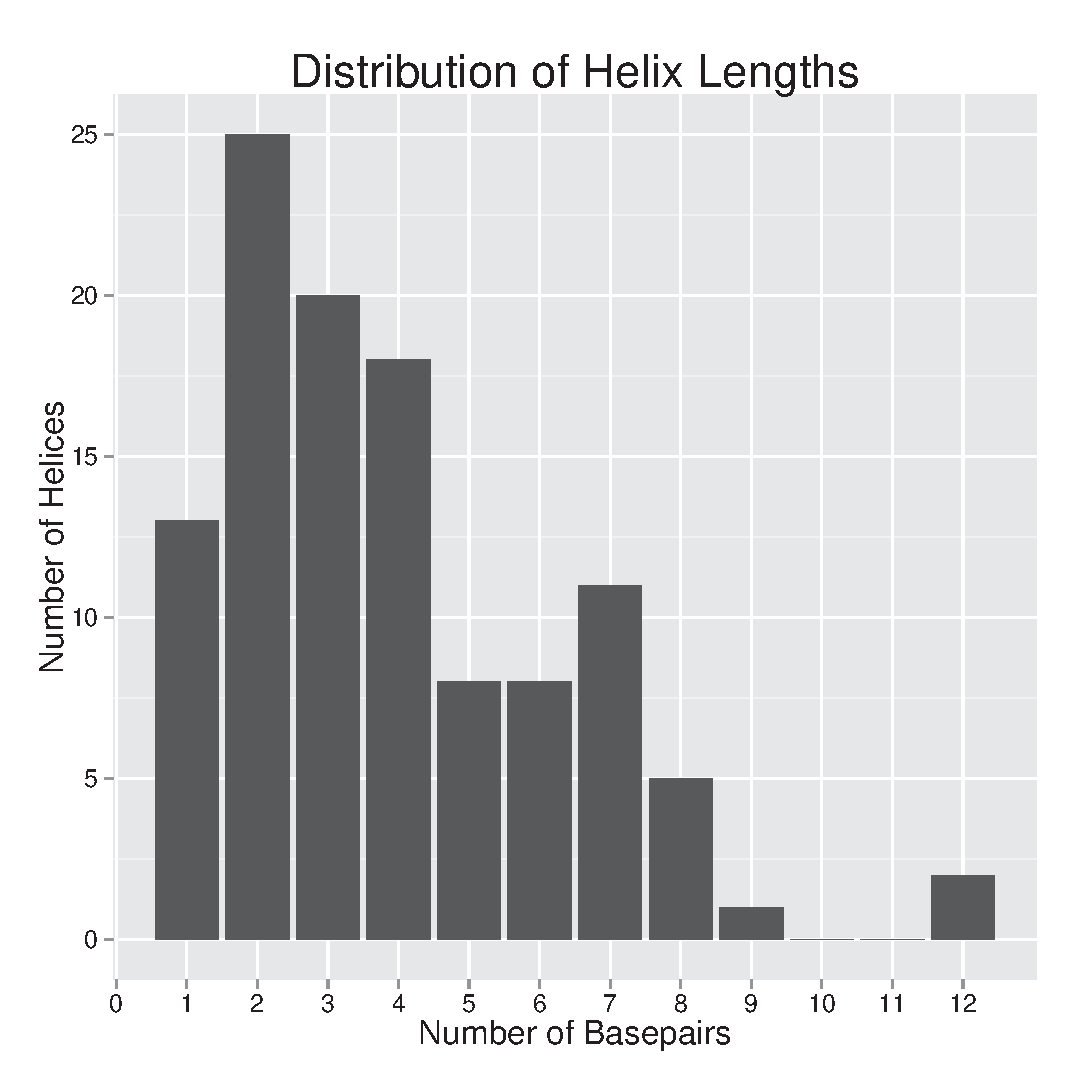
\includegraphics[width=0.5\linewidth]{chapter-1/figs/helix-lengths.eps}
  \caption{Distribution of Helix Lengths in 16S rRNA\@. Histogram of helix lengths
    (in base pairs) from the 2D representation of 16S rRNA in
  Figure~\ref{fig:ec-ssu-2d-3d}, using definitions of helices explained in the
text.}
\label{fig:ec-helix-lengths}
\end{figure}

Figures~\ref{fig:ec-hl-sizes} and~\ref{fig:ec-il-sizes} show the size
distributions of HL and IL in 16S rRNA\@. Many HL in 16S rRNA comprise 4 nts and
almost all of these are recurrent GNRA or UNCG type loops~\cite{Woese1990a}. The
smallest HL is just 2 nts. In this loop, the closing base pair is Watson-Crick
and is not counted as part of the HL\@. Recurrent GNRA and UNCG HL are closed by
non-WC paired nts, which are counted as parts of these loops; therefore, GNRA
and UNCG HL also have just two unpaired nts. 

\begin{figure}
  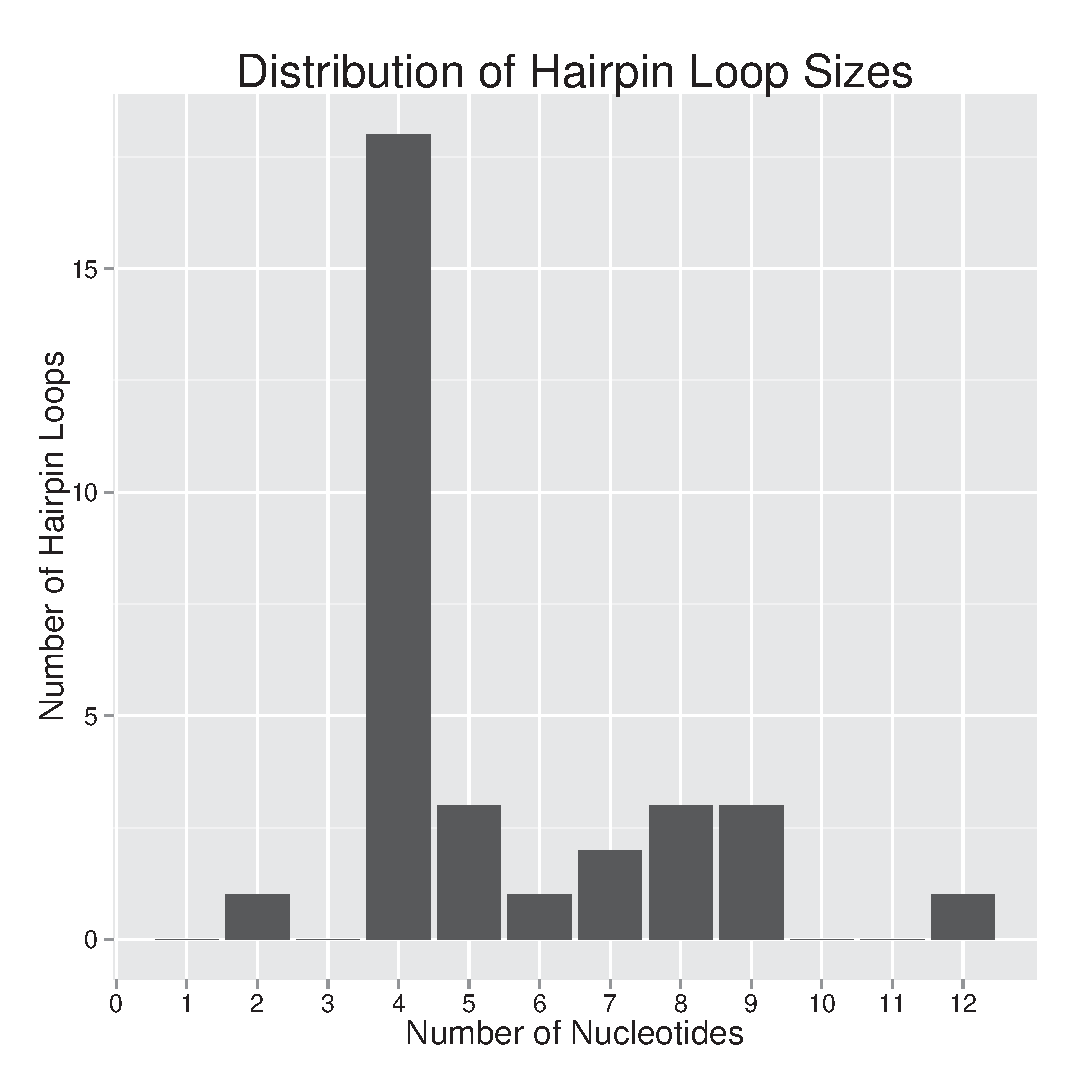
\includegraphics[width=0.5\linewidth]{chapter-1/figs/hl-sizes}
  \caption{Distribution of Hairpin Loop Sizes in 16S rRNA\@. Histogram of HL sizes
    (in nts) from the 2D representation of 16S rRNA in
  Figure~\ref{fig:ec-ssu-2d-3d}.}
\label{fig:ec-hl-sizes}
\end{figure}

\begin{figure}
  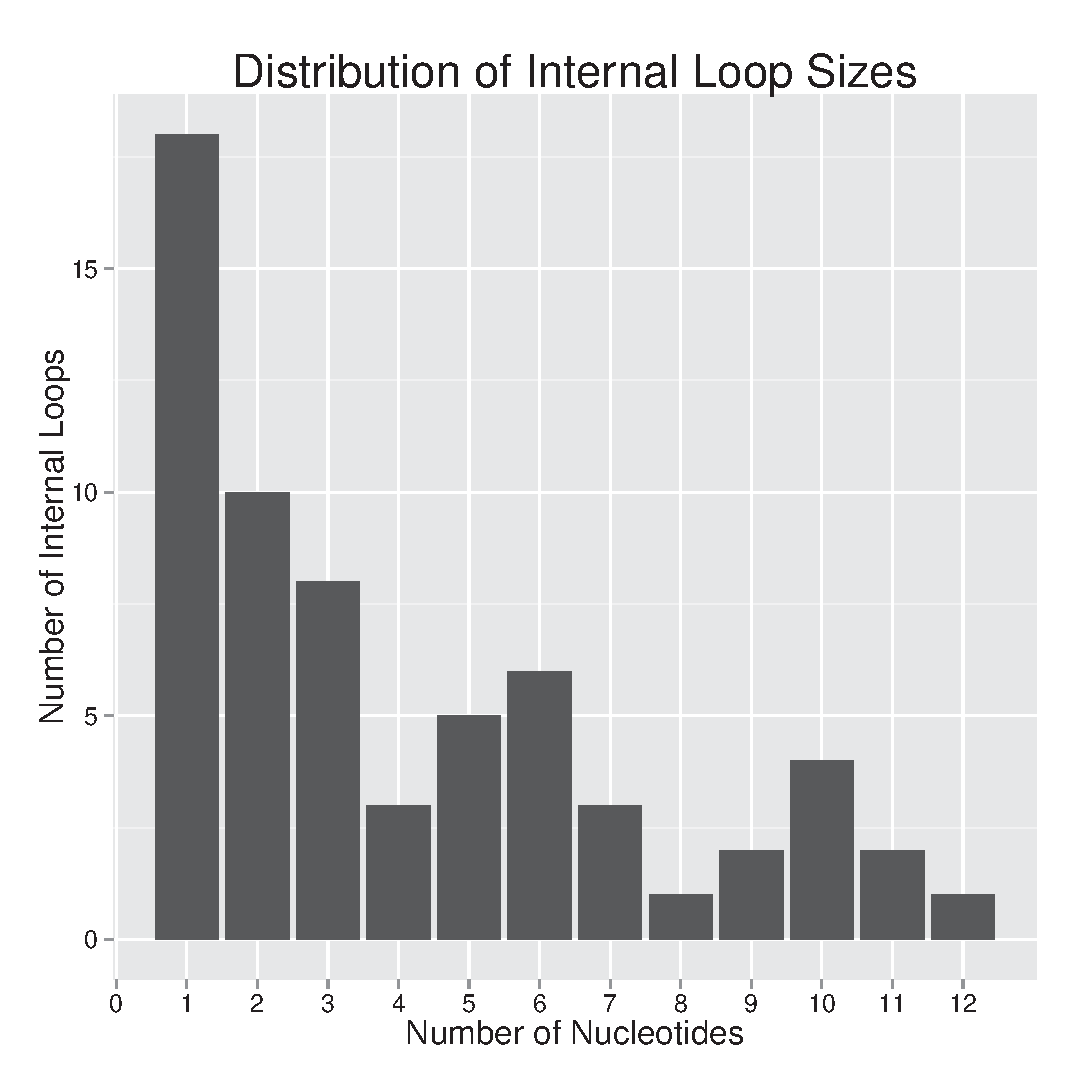
\includegraphics[width=0.5\linewidth]{chapter-1/figs/il-sizes}
  \caption{Distribution of Internal Loop Sizes in 16S rRNA\@. Histogram of IL
  sizes (in nts) from the 2D representation of 16S rRNA in
  Figure~\ref{fig:ec-ssu-2d-3d}.}
\label{fig:ec-il-sizes}
\end{figure}

The smallest IL consists of just one ``bulged'' nt, flanked on each side by
Watson-Crick base pairs. There are several of these in 16S rRNA and almost all
of them are very conserved~\cite{Gutell1994}. The 2D diagram implies that each
of these is ``bulged'' out. While the 3D structure shows that some are indeed
bulged out, others form specific interactions with the adjacent WC base pairs or
intercalate between them. Thus, even the simplest IL, drawn identically in 2D
diagrams, give rise to different, geometrically distinct 3D motifs. IL having
two nts can be symmetric (1$\times$1), with one nt in each strand, or asymmetric
(2$\times$0) with both loop nts in one strand. Again, each of these 2D motifs
gives rise to different, structurally distinct 3D motifs. To classify loop
motifs in functionally meaningful ways, the types of interactions that the loop
nts form among themselves must be considered. Using this approach, all HL and IL
loops extracted from unique NDB structures have been classified by structural
similarity and organized into an RNA Motif Atlas~\cite{Petrov2013}. The RNA
Motif Atlas can be accessed through the redesigned NDB website
\cite{CoimbatoreNarayanan2014}, and will be discussed in the last section of
this review.

\subsubsection{Interactions of loop nucleotides}

Using 16S rRNA as an example, it was shown in the previous sections that
substantial fractions of nts in structured RNAs belong to ``loops'' and these
vary in size and structure. Next, we examine the roles that loop nts play in RNA
3D structures. Figures~\ref{fig:ec-bp-loop-v-helix}
and~\ref{fig:ec-inter-loop-v-helix} provide histograms to compare the number of
interactions involving loop vs.\ helix nucleotides.
Figure~\ref{fig:ec-bp-loop-v-helix} shows base pair interactions and
Figure~\ref{fig:ec-inter-loop-v-helix} shows all annotated inter-nucleotide
interactions, including base-pairing, base-stacking and base-phosphate
interactions. Each type of interaction will be described in more detail below.
Two important points emerge from Figure~\ref{fig:ec-bp-loop-v-helix}: (1) More
than 50\% of ``loop'' nucleotides form one or more base pairs. (2) A significant
fraction (9\%) of helix nts makes one or two additional base pairs, in addition
to the defining Watson-Crick pair each forms. The additional base pairs involve
base edges other than the Watson-Crick edge and are, by definition, non-WC
pairs. In no case do bases make more than three base pairs, for reasons
explained below.

\begin{figure}
  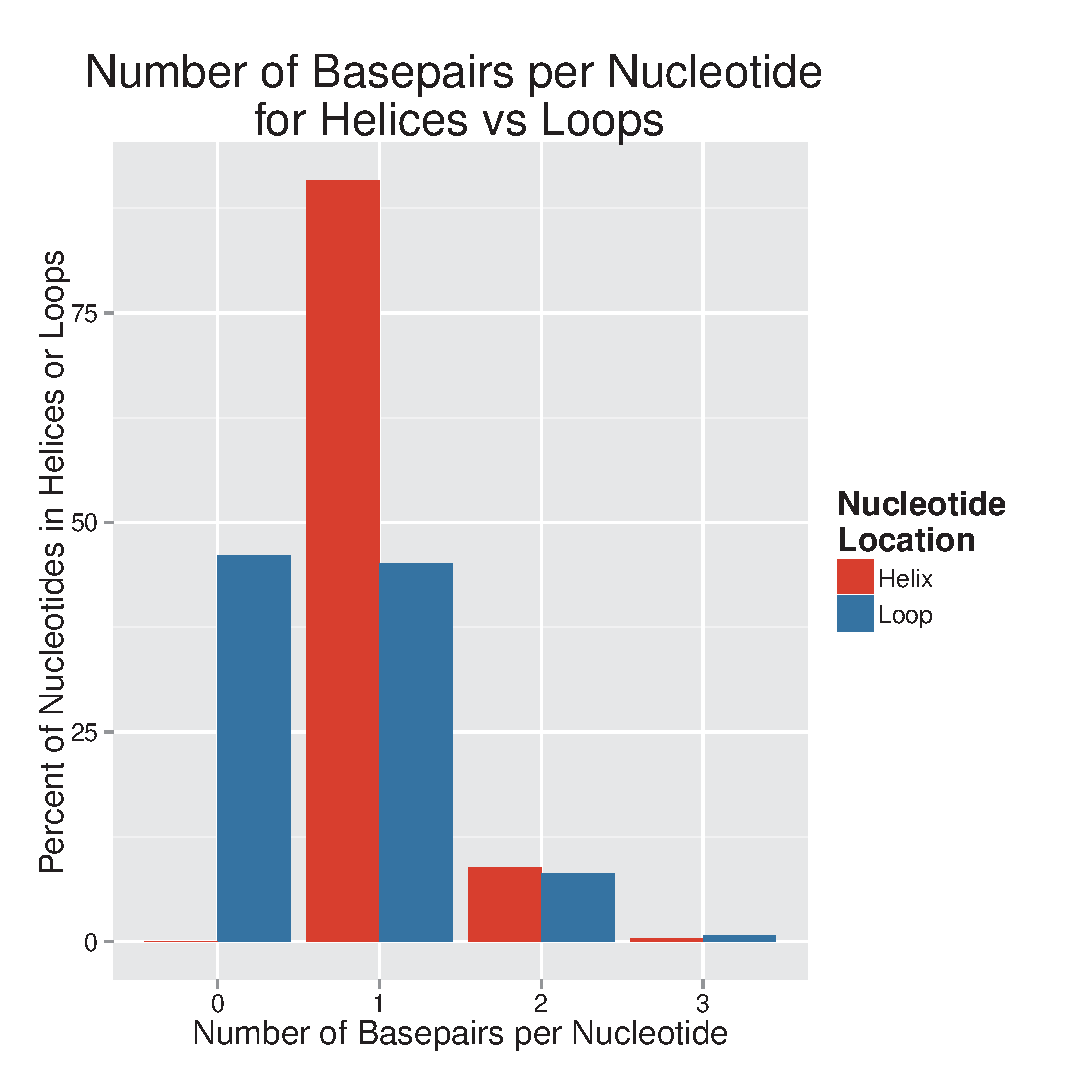
\includegraphics[width=0.5\linewidth]{chapter-1/figs/bp-loop-v-helix}
  \caption{Comparison of Base pairs formed by Nucleotides in Loops vs.\ Helices.
    Histogram comparing number of base pairs (non-WC as well as WC) formed by
  nucleotides in loops (blue) vs.\ helices (red).}
\label{fig:ec-bp-loop-v-helix}
\end{figure}

\begin{figure}
  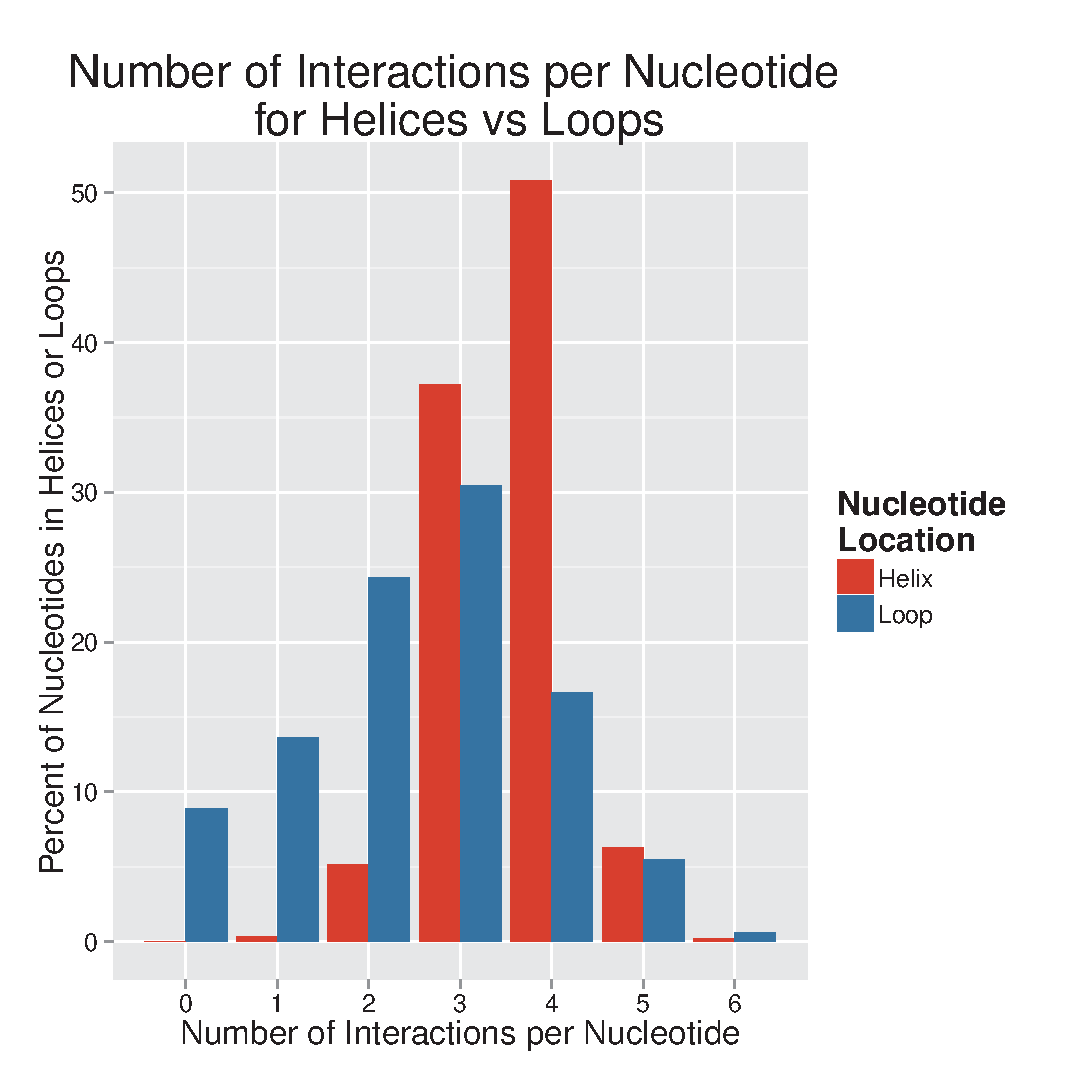
\includegraphics[width=0.5\linewidth]{chapter-1/figs/inter-loop-v-helix}
  \caption{Comparison of Interactions formed by Nucleotides in Loops vs.
  Helices. Histogram comparing number of annotated interactions (base-pairing,
base-stacking, and base-phosphate) formed by nucleotides in loops (blue) vs.\ helices (red).}
\label{fig:ec-inter-loop-v-helix}
\end{figure}

Figure~\ref{fig:ec-inter-loop-v-helix} shows that when we include stacking and
base-phosphate interactions, most nts in the 16S structure, whether they are
found in loops or helices, form two or more interactions. As expected, most
helix nts form 3 or 4 interactions, corresponding to one base pair and 2 or 3
stacking interactions per nt. Even nts on the ends of helices stack on at least
one other base. Thus, almost all helical nts have at least two interactions, one
pairing and one stacking. With regard to loop nucleotides,
Figure~\ref{fig:ec-inter-loop-v-helix} shows that almost 80\% form two or more
interactions with other nts in 16S rRNA | evidence that most loops form specific
structures. On average, nucleotides in loops form
2.5 interactions per nt compared to 3.6 for those in helices. The stacking data
(not shown) shows that 85\% of loop nts form one or more stacking
interactions, with >60\% forming two or more; on average, loop nts form 1.7
stacking interactions per nucleotide, compared to 2.5 for helix nts. 

Less than 15\% of loop nts form only 1 interaction and, surprisingly, only \TILDE 58
loop bases in 2AW7, or less than 4\% of all nts in this 16S rRNA structure, form
no classified pairing, stacking or base-backbone interactions and are candidates
for bases that completely “bulge out” of the structure, as implied by 2D
diagrams for all loop nts. Detailed analysis of 3D structures of ribosomes in
different states shows that most of these 58 bases do in fact form some kind of
interaction by stacking or H-bonding to tRNA, mRNA or 23S rRNA, by binding to
ribosomal proteins, or by forming as yet unannotated or unclassified base-ribose
or perpendicular base-base interactions with other nts (Roy et al., unpublished
observations). Classification of base-ribose and perpendicular interactions is
an active area of research (Zirbel, private communication); once classes of
interactions are agreed upon, these interactions will also be annotated in NDB\@. 

Regarding base-phosphate (BPh) interactions, which are the most sequence
specific base-backbone interactions, less than 4\% of helical nucleotides (34 of
866) provide the base in such interactions, whereas 18.4\% of loop bases do so
(122 of 664). In addition, 18\% of loop nts provide the phosphate groups for BPh
interactions but only 4\% of helix nts do so. This shows that loop nts also play
a prominent role in mediating BPh interactions, which contribute substantially
to stabilizing folded RNA structures~\cite{Zirbel2009, Sponer2010}. 

Taken as a whole, these data show that nts in loops and linkers form significant
numbers of interactions of all types and therefore loop regions are generally
well structured and contribute significantly to RNA 3D structure. Next we
analyze these interactions in more detail to identify the locations of
interacting nucleotides. 

\subsection{Local vs.\ long-range interactions in loops and helices}

To better understand the roles of loop and linker nts in RNA 3D structure, we
next address these questions: How many structure-stabilizing interactions occur
between loop nts, how many between helical nts, and how many between loop and
helical nts? How many of these interactions contribute to local structure and
how many to the overall 3D architecture? To answer these questions it is useful
to classify interactions according to whether they are local or long-range.
Long-range interactions are of particular interest because they contribute to
the overall folding of structured RNA molecules. Before presenting the data, we
discuss how local and long-range interactions can be distinguished by automated
means to facilitate structural analysis (Zirbel, private communication). 

\subsubsection{Defining long-range (LR) interactions}

Local interactions are those between nts belonging to the same helix or loop, or
between adjacent elements of the 2D structure, while LR interactions are those
between nts distant in the 2D\@. The farther apart two nts are in the 2D
structure, the more WC base pairs they ``cross over'' when they interact. By
definition, all of the WC base pairs that define the 2D structure are ``nested''
with respect to each of the others.  Two WC pairs (i,k) and (m,n) are nested
when either i \textgreater{} m \textgreater{} n \textgreater{} k (as shown in
Figure~\ref{fig:nesting}A) or m \textgreater{} i \textgreater{} k \textgreater{} n,
where i, k, m and n are the nt numbers in the linear RNA sequence (given in the
5’ to 3’ direction) and i \textgreater{} k, m \textgreater{} n. In other words,
nested interactions do not cross over each other in the 2D structure. On the
other hand, if two interactions (i,k) and (m,n) are such that i \textgreater{} m
\textgreater{} k \textgreater{} n, as shown in Figure~\ref{fig:nesting}B, or
alternatively, m \textgreater{} i \textgreater{} n \textgreater{} k, then they
``cross.'' Once a comprehensive set of nested WC pairs is identified and
assigned to the 2D structure, one can measure how ``local'' or ``LR'' any other
interaction is, by counting the number of nested WC pairs it crosses over. This
measure is called the “crossing number,” and the larger it is, the more distant
the interacting nts are in the 2D structure.  By definition, all WC pairs that
belong to the 2D structure have crossing number equal to zero. An example of an
interaction (x,y) that crosses two nested Watson-Crick pairs, (i,j) and (m,n),
is shown in Figure~\ref{fig:nesting}C\@. The pair (x,y) has crossing number equal
to two. Whether interactions are labeled local or LR depends on the choice of
cutoff for the crossing number. Certainly, the cutoff should be $\ge 1$, so that
interactions with crossing number zero are labeled ``local.'' The smaller the
cutoff, the more interactions will be defined as LR, but if the cutoff is set
too low, interactions between nts that are very close to each other in the 2D
structure and best considered local, will be labeled LR\@. If the cutoff is set
too high, interactions best classified as LR will be labeled local. We find that
a cutoff equal to four provides a good compromise, so we label all interactions
with crossing number $\ge 4$ ``LR'' (Zirbel, private communication). 

\begin{figure}
  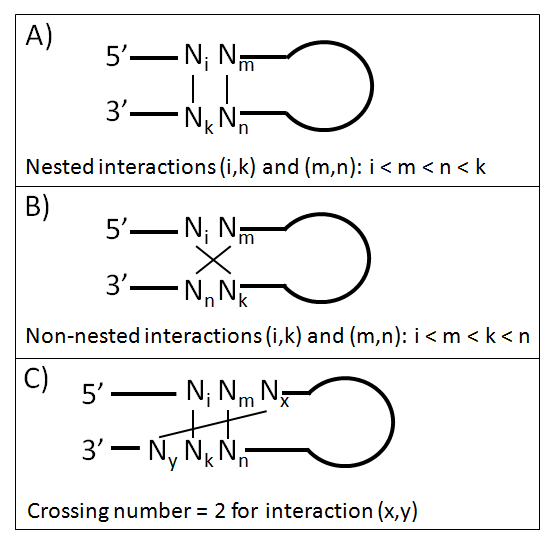
\includegraphics[width=0.5\linewidth]{chapter-1/figs/nested}
  \caption{Definition of Crossing Number for Long-range Interactions. Base pairs
    (i,k) and (m,n) are nested in (A) but non-nested in (B). Interaction (x,y)
    in (C) crosses over two nested base pairs, (i,k) and (m,n) and has crossing
  number equal to 2.}
\label{fig:nesting}
\end{figure}

\subsubsection{Local vs.\ long-range (LR) interactions in 16S rRNA}

Using crossing number $\ge 4$, we find 163 LR interactions in 16S rRNA\@. The
relevant data for \EC{} 16S rRNA are presented in
Table~\ref{tab:helix-loop-inter}. Not surprisingly, most nt interactions are
local (2323 local vs.\ 163 long-range) and most of these are between two nts in
the same or adjacent helices (1323 out of 2323 or 57\%); however, almost 24\% of
local interactions are between nts in the same or nearby loops (552/2323) and
19\% (448/2323) involve nts in adjacent loops and helices. Most such local
loop-helix interactions are base stacking (386 of 448 or 86\%), indicating that
loop nts frequently stack with the WC pairs of adjacent helices. Many of these
helices appear in the 2D to be very short, comprising only one or two base pairs
(see Figures~\ref{fig:ec-ssu-2d-3d} and~\ref{fig:ec-helix-lengths}). Thus, for
the most part, these very short helices are not isolated but are stabilized by
stacking on bases in the adjacent HL, IL or MHJ loops, many of which form non-WC
base pairs. In fact, 16S rRNA contains 15 local AG cis Watson-Crick (cWW) base
pairs, most of which occur at the interfaces between loops and helices. Readers
should note that cWW pairs composed of non-canonical base combinations (i.e.\
other than AU or GC) are considered non-WC pairs. These and other non-WC pairs
can be considered to form extensions of the secondary
structure~\cite{Gutell1990}. Local stacking interactions also play major roles
in loops; they account for 336/552 or 61\% of interactions within loops. In
fact, 336/1600 (22\%) of all local stacking interactions occur in loops. 

\begin{landscape}
\begin{table}
  \begin{tabulary}{\linewidth}{LRRRRRRRRR}
    \toprule
                & \multicolumn{4}{c}{Local Interactions}               & \multicolumn{5}{c}{Long-Range Interactions} \\
    \cmidrule(r){2-5}                                       \cmidrule(r){6-10}
                & Base-Pairing & Base-Stacking & Base-Phosphate & Subtotals & Base-Pairing & Base-Stacking & Base-Phosphate & Helix Packing & Subtotals \\
    \midrule
    Helix-Helix & 440 & 878 & 5 & 1323 & 0 & 0 & 6  & 5 & 11 \\
    Helix-Loop  & 38 & 386 & 17 & 448 & 42 & 6 & 6  & & 70 \\
    Loop-Helix  &    &     & 7  &     &    &   & 16 & &  \\
    Loop-Loop   & 135 & 336 & 81 & 552 & 35 & 34 & 18 & & 87 \\
    Totals      & 613 & 1600 & 110 & 2323 & 77 & 40 & 46 & & 168 \\
    \bottomrule
  \end{tabulary}
  \caption{Interactions between helix and loop nts, local vs.\ long-range.
    Analysis of interactions between nts in helices, in loops and between loops
    and helices. Interactions are classified as long-range if they cross four or
    more nested WC base pairs. All other interactions are local. Base-phosphate
    interactions are separated, depending on whether the helix or loop nt
    contribute the base to the interaction, ``Helix-Loop'' and ``Loop-Helix'',
  respectively.}
\label{tab:helix-loop-inter}
\end{table}
\end{landscape}

As concerns local pairing and base-phosphate interactions in loops, most of
these occur between nts in the same or adjacent loops and far fewer with nts in
helices (135 local loop-loop vs.\ 38 local loop-helix base-pairing interactions
and 81 local loop-loop vs.\ 24 local loop-helix BPh interactions). 

While there are far fewer LR than local interactions within 16S rRNA, the LR
contacts are crucial for defining and stabilizing the 3D architecture. The
absolute numbers depend, of course, on the value of the crossing number cutoff
used, as discussed above. In generating the data reported here, we used cutoff =
4. With this cutoff, most LR interactions occur between nts distant in the 2D
structure, i.e.\ nts belonging to different helical elements and even
different structural domains. While 76\% of local interactions involve helix
nts (1771 of 2323 interactions), 93\% of long-range interactions involve loop
nts (157 of 168) of which 52\% (87 of 168) are between two loop nts.  Only
11/168 or 6.5\% of long-range interactions are between two helix nts and all
of these are BPh or helix packing  (``P-'') interactions~\cite{Mokdad2006b}.
The latter involve highly conserved GU pairs that interlock on their sugar
edges with AU or GC WC pairs and occur exclusively between helices, forming
crucial highly conserved inter-helical tertiary contacts in structured RNAs
\cite{Gagnon2006, Gagnon2002}. 

Table~\ref{tab:helix-loop-inter} shows that LR loop-loop interactions include
comparable numbers of pairing, stacking and BPh interactions, while LR
loop-helix interactions are dominated by non-WC base pairing. Most of these
involve the sugar edges of the helix nts (see below). 

In base-phosphate (BPh) interactions, one nt contributes the base and the other
the phosphate group. The base-phosphate interactions are separated in
Table~\ref{tab:helix-loop-inter} according to whether the helix or loop nt
contributes the base to the interaction. The row in
Table~\ref{tab:helix-loop-inter} labeled ``Helix-Loop'' includes interactions in
which the helical nts contribute the base and vice versa for the row labeled
``Loop-Helix''. These data show that the loop nt usually provides the base in LR
loop-helix BPh interactions, whereas this is reversed in local interactions.
There are comparable numbers of LR base-pairing and LR BPh interactions between
loops and helices as between two loop nts, but far more LR stacking interactions
between two loop nts than between loop and helix nts interactions (34 vs.\ 6). 

\subsubsection{Base-stacking interactions of loop nts}

What kinds of stacking interactions are observed in loops? As in helices, there
is stacking between consecutive bases in the same strand, but in loops there are
additional types of stacking. In many loops, there is extensive “cross-strand”
stacking between bases forming consecutive non-WC base pairs but located in
opposite strands. Cross-strand stacking is a characteristic feature of many RNA
3D motifs, including recurrent sarcin-ricin motifs~\cite{Szewczak1993a}.
Extensive stacking is also observed between helical elements that meet at MHJ\@.
As helices at MHJ can stack in different ways, the pattern of inter-helix
stacking is a defining feature of each MHJ\@. Thus, stacking at junctions is a
local interaction with important implications for the global RNA architecture
\cite{Lescoute2006b}. 

Among LR interactions, stacking occurs between the apical bases of certain HL,
most commonly GNRA loops, and the IL forming ``platform'' or loop receptor motifs
\cite{Cate1996}. LR stacking interactions reinforce tertiary base-pairing and
base-phosphate interactions to anchor the docking of these loops to their
receptors. LR tertiary (3°) stacking interactions between two “bulged out” bases
also occur to stabilize the compact folding of the RNA\@. 

Finally, intercalation of a bulged base from one loop into a binding site
created by another loop results in two or more LR stacking interactions and
generally at least one LR pairing or BPh interactions. The interaction between
the D- and T-loops of tRNA involves intercalation of bulged bases from the
D-loop in the T-loop~\cite{Quigley1976}. All T-loop HL motifs provide sites for
intercalation of a bulged base from another loop~\cite{Nagaswamy2002}. 

\subsubsection{Quaternary Interactions of 16S rRNA}

Most, if not all, cellular RNAs interact specifically with one or more protein.
\EC{} 16S rRNA associates with 21 different ribosomal proteins (r-proteins) to
form the small (30S) ribosomal subunit or ``SSU,'' and transiently with several
translation factors. Figure~\ref{fig:aa-loop-v-nt} shows a histogram of SSU
protein-RNA interactions for loop and helix nts in 16S rRNA (PDB file 2AW7).
About 60\% of nt-amino acid interactions involve loop nts, even though loop nts
constitute just 42\% of all 16S nts, demonstrating once again the important role
of loop nts in the functional interactions of structured RNA\@.

\begin{figure}
  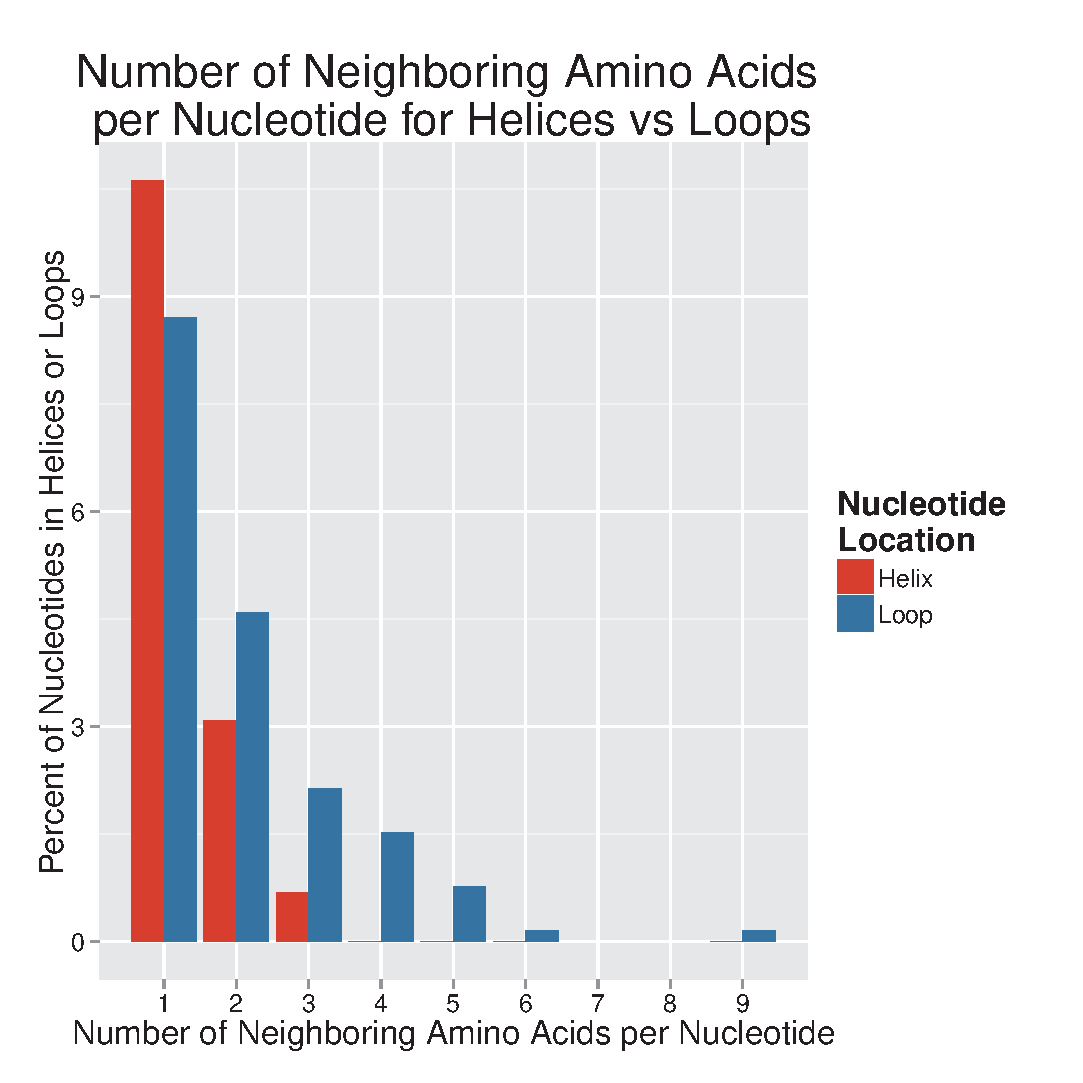
\includegraphics[width=0.5\linewidth]{chapter-1/figs/aa-loop-v-nt}
  \caption{Amino Acid Interactions for Loop vs.\ Helix Nucleotides. Histogram of
    number of amino acids within 4Å for nucleotides in loops (blue) vs helices
    (red) in \EC{} 30S ribosome. }
\label{fig:aa-loop-v-nt}
\end{figure}

The 30S particle also interacts with the large (50S) ribosomal subunit, or LSU,
to form the functional 70S ribosome. Non-covalent interactions or ``bridges''
that form between the subunits, many of which involve RNA, stabilize the
assembled 70S ribosome~\cite{Yusupov2001}. Most of the 16S nts interacting with
the LSU are loop nts or helix nts adjacent to loops. 

About thirteen of the approximately 58 ``bulged out'' nts that do not interact
with other nts in \EC{} 16S rRNA, interact with SSU protein molecules. From
structures that contain bound mRNA and tRNA we observe that three others
interact with tRNA, three with mRNA, and A532, which is bulged out in 2AW7,
forms a bridge to the head domain of 16S when the head clamps down on the mRNAs
and the tRNA bound to the 16S A-site. Another bulged base, U723 forms a
base-phosphate interaction with the mRNA-Shine-Delgarno helix. A702, which
bulges out of the H23 kink-turn, interacts with 23S rRNA\@. Five others of these
58 ``looped out'' bases form perpendicular base-base interactions and eight form
base-ribose interactions. In summary only about half of the 58 nts (less than
thirty) are truly bulged out and of these \TILDE 21 facilitate tight turns in the 16S
backbone, of which 7 are in UNCG loops. 

The conclusion of this overview of the prevalence and roles of loop nts,
exemplified by 16S rRNA, is that almost all nts, whether they belong to ``loops,''
linkers, or helices in the 2D structure, form some kind of pairing, stacking or
base-backbone interactions. Moreover, interactions of loop nts constitute most
of the crucial long-range pairing, stacking and base-phosphate interactions that
stabilize domain structures and architectures and mediate most interactions with
proteins and other RNAs. Most of the very small number of truly “looped out”
bases play a role in facilitating formation of sharp \TILDE 180\degree turns in the RNA
backbone. 

For completeness, we conclude this section by briefly explaining the criteria
used to assign nts to helices and loops in a consistent way that can be applied
to analyze other structures and to automatically extract loop motifs for
detailed comparison and analysis.  This will help readers better understand how
motifs are extracted from structures for the RNA 3D Motif Atlas~\cite{Petrov2013}, now
accessible through the revised NDB website~\cite{CoimbatoreNarayanan2014}. 

\subsection{Assigning nts to helices and loops in structured RNAs}

While it is usually clear from accurate 2D diagrams, drawn with reference to 3D
data, whether a given nt should be assigned to the 2D structure, or to linkers,
HL, IL or MHJ loops, there are ambiguous cases that require clear definitions to
obtain consistent assignments. First, the choice of which helices to count as
Pseudoknots (PK) and which as part of the 2° structure is to some degree
arbitrary and different choices will also change the number of HL, IL, MHJ
loops, and linker regions~\cite{Smit2008}. For example, if helix 2 (formed by
interactions between nts in the HL of helix 1 and the linker joining helices 27
and 28) is included in the 16S 2D, then H1 becomes the PK and a new 4-way
junction is defined, comprising H2, H3, H19 and H27. To build a comprehensive
Motif Atlas, it may be necessary, for each 3D structure, to cycle systematically
through alternative PK definitions to identify all motifs. Generally, the helix
formed by nts closest in the primary sequence is given precedence. Following
this guideline, helix 1 is favored over helix 2 for inclusion in the 2D\@. 

Second, there may be structural differences between PDB/NDB files for the same
RNA molecule. These differences can be due to inconsistencies or errors in the
3D modeling~\cite{Stombaugh2009}, or to bona fide structural changes that occur
upon binding of substrates or other ligands. Furthermore, some regions of RNA
molecules are so dynamic that it is not possible to build unique
atomic-resolution models for them. In these cases, the structure must be
inferred by combining other data, including CSA, 3D modeling and structural
studies of RNA fragments. 

Even where all 3D structural models agree, further questions arise regarding how
to partition structures into helices and loops, including:

\begin{enumerate}
  \item Should single (isolated) Watson-Crick pairs that occur between two loops
    be assigned to the loops or to the 2D structure? 

  \item Should GU ``wobble'' pairs always be assigned to the 2D regardless where
    they are located? 

  \item How should other cis Watson-Crick pairs (AA, AC, AG, CC, CU and UU) be
    treated, especially when these form interfaces between helices and loops? 
\end{enumerate}

\subsubsection{Isolated Watson-Crick pairs}

Not infrequently, a single WC pair separates two loops. In which cases should
the WC pair be assigned to one of the adjacent loops and when should it be
considered part of the 2D structure? Alternatively, should the loops be merged
into a single 3D motif and the WC pair treated as belonging to this larger
motif? Examples of such “isolated” Watson-Crick base pairs in 16S rRNA occur
between IL in H17 and in H44 and between IL and MHJ loops in H5, H19, H22, H23,
H33, H40, and H42. 

The solution we propose is to treat loops separated by single WC pairs as
separate 3D motifs and assign the WC pair to the 2D, unless the nts of this WC
pair form extensive interactions with nts of each of the adjacent loops. In the
case of the H17 and H44, the interactions of the WC pairs are limited to base
stacking with neighboring bases in the sequence. In these cases the sequence of
the WC pair is less likely to be conserved and typical WC co-variation is
usually observed, and the adjacent loops are best treated as distinct motifs
with the WC pairs assigned to the 2D structure. However in the case of IL
adjacent to five of the MHJ loops of 16S rRNA there are additional interactions
involving the embedded WC pairs. Moreover, these pairs tend to be highly
conserved in sequence, due to the additional interactions. In these cases we
propose that the WC pair should be assigned to the MHJ loop and not to the 2D
structure. This was done in constructing Table~\ref{tab:ec-element-count}. All
the WC pairs marked with red lines in Figure~\ref{fig:ec-ssu-2d-3d}  are of this
type. 

\subsubsection{GU cWW pairs}

Sequence analysis shows that most cWW GU pairs in an RNA structure co-vary with
AU, UA, GC, and CG in homologous sequences, indicating that at these positions
GU pairs are functionally indistinguishable from WC pairs. Therefore we assign
cWW GU pairs that are adjacent to HL, IL, or MHJ loop motifs to the 2D
structure, just as is done for AU and GC pairs. This is the approach taken in
the construction of the 3D Motif Atlas~\cite{Petrov2013}. Nonetheless, readers
should note that sequence analysis shows that highly conserved cWW GU base pairs
flank some HL, IL and MHJ loop motifs and perhaps these should be considered
parts of these motifs, at least operationally, for example, in designing
self-assembling RNA molecules for RNA nanotechnology or in 3D structure
prediction. This is an area of current research that requires integration of
comparative sequence analysis and biophysical characterization. In fact, in a
number of 3D motifs, exemplified by C-loops, the flanking WC pairs actually form
base triples with the loop nts, and therefore could be considered part of the
motif~\cite{Lescoute2005}. Even though the RNA 3D Motif Atlas extracts each loop
motif together with its flanking Watson-Crick pairs to facilitate analysis of
their interactions and their sequence variations, the flanking WC pairs are
still considered part of the 2D structure~\cite{Petrov2013}. 

\subsubsection{AG, AC and other cWW pairs}

AG \emph{cis} Watson-Crick (cWW) pairs are not uncommon in structured RNAs; they
tend to occur at the ends of helices flanking loop motifs, especially MHJ motifs
[27]. They rarely occur within helices because they are larger than AU or GC WC
pairs and therefore not isosteric to them, and when substituted for them,
distort the local helical geometry and destabilize adjacent WC base pairs.
Because cWW AG pairs almost always occur adjacent to loops and rarely co-vary
with GC or AU, we assign all cWW GA pairs to the loops rather than the adjacent
helices, consistent with the way they are treated in the 3D Motif Atlas. For
consistency, other non-WC cWW base pairs, including AC, AA, UU, CU, and CC, are
also treated this way.

In the next section we describe the components of RNA nucleotides to provide a
basis for understanding nucleotide-level interactions in RNA\@. 

\section{Components of RNA nucleotides}

The nucleotide is the basic unit of RNA structure. It is also the synthetic unit
or “synthon” from which RNA is produced in vivo. Each nucleotide is made of one
of the four RNA bases, Adenine (A), Cytosine (C), Guanine (G), or Uracil (U),
attached to ribose, a 5-membered sugar ring, which in turn is linked to one or
more phosphate groups. 

Two features distinguish RNA from DNA and have important structural
implications: the substitution of -OH at the 2'-carbon of the ribose ring in RNA
in place of -H in the deoxy-ribose ring of DNA, and the substitution of uracil
(U) in RNA for thymidine (T) in DNA\@. The 2’-OH facilitates H-bonding along the
``Sugar-edge'' of each RNA nt. U lacks the 5-methyl group of Thymidine (T),
located on the Hoogsteen edge of T; consequently U, but not T, can form base
pairs along its Hoogsteen edge. These structural differences make RNA more
versatile than DNA in forming interactions that support complex structures.

\subsection{Bases and Base Edges}

Each base is a nitrogen-rich, heterocyclic aromatic ring system that is planar
in its equilibrium geometry and quite rigid, due to delocalization of
pi-electrons. RNA bases are of two types, the pyrimidines (U and C), composed of
one six-membered aromatic, heterocyclic ring, and the larger purines (A and G),
composed of fused five- and six-membered rings. Structures of nts with the
numbering of base positions are shown in Figure~\ref{fig:bases}. Base ring atoms are numbered
from 1 to 9 in purines and from 1 to 6 in pyrimidines. Exocyclic groups and
attached hydrogen atoms are numbered according to ring position. Ribose atoms
are numbered with primes, from 1' to 5', to distinguish their atoms from those
of the base. 

\begin{figure}[p]
  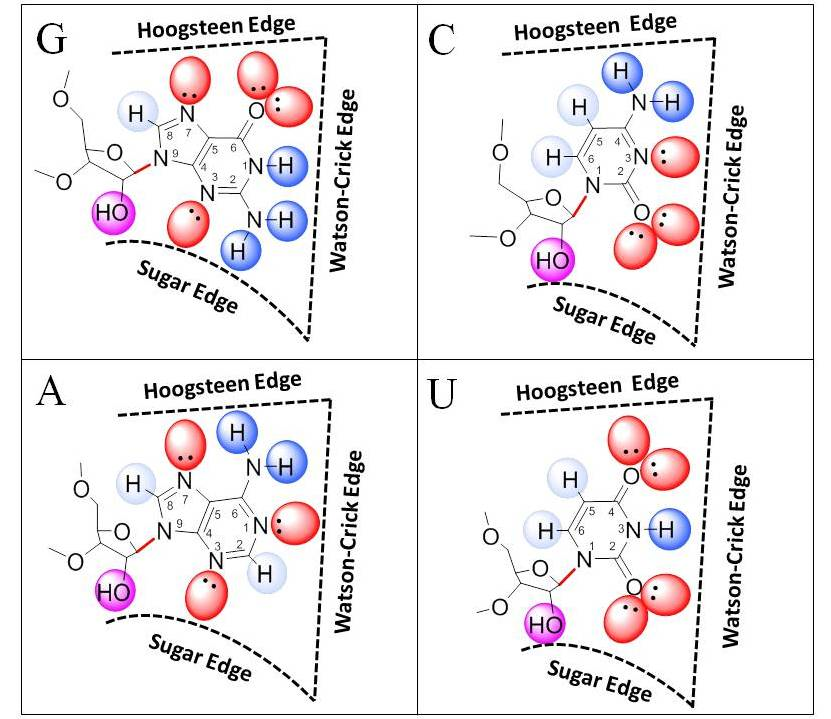
\includegraphics[width=\linewidth]{chapter-1/figs/bases}
  \caption{Structures of RNA nucleotides. RNA nts G, C, A, and U each have three
    edges along which H-bonding takes place. Hoogsteen, Watson-Crick, and Sugar
    Edges are marked with dotted lines. Base ring atoms are numbered from 1 to 9
    for purines and 1 to 6 for pyrimidines. Exocyclic groups and attached
    hydrogens are numbered according to ring position. H-bond donors are
  highlighted with blue and H-bond acceptors with red.}
\label{fig:bases}
\end{figure}

The planar RNA bases present three ``edges'' studded with H-bonding donor and 
acceptor groups along which H-bonds can form with the edges of other bases, as
well as with phosphate and ribose groups, amino acid side chains or backbone
atoms of proteins and small molecules. These edges are called the Watson-Crick
(W), Hoogsteen (H) and Sugar (S) edges~\cite{Leontis2001}. Therefore it is
useful to represent RNA bases, purines as well as pyrimidines, as triangles, or
more precisely, oblate triangular prisms to describe and classify their diverse
interactions as observed in RNA 3D structures~\cite{Hoehndorf2011}. The base
edges are indicated for each RNA base in Figure~\ref{fig:bases}. Further support for
representing bases as triangles comes from the observation that bases can pair
edge-to-edge with up to three other bases at the same time, but no more than
three~\cite{AbuAlmakarem2012b}. This explains the observation that no nt in 16S
forms more than three base pairs (see Figure~\ref{fig:ec-bp-loop-v-helix}). 

In triangles representing the RNA bases, two of the vertices coincide with
exocyclic H-bonding functional groups. The H and W edges meet at the vertex
defined by the N4 or N6 amino groups of C and A, respectively. The corresponding
atoms for U and G are the O4 and O6 carbonyl oxygen atoms. The W and S edges
meet at the vertex defined by the O2 carbonyl group in C and U, the polarized
C2-H2 of A, and the N2 amino group of G\@. The glycosidic bond connecting each
base to the C1’ carbon of the ribose defines the third vertex of the triangle,
where the H and S edges meet. The 2'-OH group, unique to RNA, extends the
H-bonding capability of the Sugar edge of each nucleotide

The RNA bases are shown in Figure~\ref{fig:bases} with H-bond donor groups
shaded with blue ``clouds'' and the H-bond acceptor groups shaded with red
``clouds,'' representing centers of positive and negative charge, respectively.
The ribose 2'-OH group is shaded in purple because it can serve as either H-bond
donor or H-bond acceptor. 

\subsection{Ribose sugar rings}

RNA bases are covalently attached to the 1'-carbons of their respective ribose
rings by single C-N bonds, the ``beta-glycosidic'' bonds. In the beta
configuration, each base is attached by the glycosidic bond to the same side of
its ribose ring as the ribose 5'-carbon atom. The ribose ring is a five-carbon
aldose sugar present in the furanose form. The flexible beta-glycosidic bonds
allow for relatively free rotation of the RNA base relative to the ribose
moiety. Rotation of the base gives rise to two distinct conformational classes
of the nucleotide, called anti and syn~\cite{Neidle2008}. In the anti
configuration the Watson-Crick edges of the bases point away from the
5’-phosphate group. In the syn configuration the base is rotated \TILDE 180\degree
about the glycosidic bond so the WC edge faces the 5'-phosphate. G is the base
that is most often observed in syn. In the syn configuration, the N2 amino group
of G can H-bond to a 5'-phosphate oxygen atom. However, in polynucleotides, the
anti configuration is much more common. The anti configuration is stabilized by
weak H-bonding of the purine H8 or pyrimidine H6 atoms on the Hoogsteen edge to
the 5'-phosphate group. Whether a base is syn or anti affects the kinds of base
pairs it can form with nearby bases. One of the most common discrepancies
between published RNA 3D structures of the same molecule is the glycosidic bond
configuration of certain nts~\cite{Leontis2002f}. 

\subsection{Phosphate groups}

Phosphate groups are derived from phosphoric acid (\ce{H3PO4}), a weak acid with
three dissociable protons that can form up to three phospho-ester linkages. In
RNA and DNA, there is one phosphate per base-sugar unit (``nucleoside'') and
each phosphate links two nucleosides, by forming two phospho-ester bonds. Each
phosphate is arbitrarily assigned to the nt to which it is attached at the
5’-hydroxyl group. The phosphate groups link adjacent nucleoside units to each
other by forming second linkages to the 3'-hydroxyls of the preceding one in the
linear chain. To link two nucleosides together, each phosphate loses two protons
(\ce{H+}) and forms two electrically neutral phospho-ester linkages. The
remaining proton is acidic and largely dissociates at neutral pH\@. Therefore each
phosphate group in RNA carries a full negative (-1) electrical charge, which is
delocalized over the two non-bridging oxygen atoms of the phosphate group,
making them strong H-bond acceptors. Consequently, base-phosphate interactions
play structurally important roles and can be as stabilizing as GC base pairs
\cite{Zirbel2009, Sponer2010}. Large RNA molecules like 16S rRNA, therefore,
have substantial negative charge that must be neutralized by H-bonding
interactions or mobile positive ions in order for the RNA to fold into its
functional structure. In vivo, charge neutralization depends on \ce{Mg2+},
assisted by basic proteins and polyamines~\cite{Draper2008}.

\subsection{RNA Backbone Conformations}

The backbone of the RNA chain is very flexible and able to assume many different
conformations because each nt contributes six covalent single bonds, including
the C3'-C4' and C4'-C5' bonds of the ribose ring and two C-O and O-P bonds
comprising the two phospho-ester linkages. The conformation of each nt is
defined by the set of values of the dihedral angles of these bonds together with
that of the glycosidic bond~\cite{Neidle2008}. The dihedral angles of each Nt
are assigned Greek letters, alpha ($\alpha$) to zeta ($\zeta$), starting with
the P-O5' bond of the 5'-phosphate and continuing consecutively with the
O5'-C5', C5'-C4', C4'-C3', C3'-O3', and ending with the O3'-P bond of the
3'-phosphate. The glycosidic bond (``chi'' or $\chi$) contributes the seventh
dihedral angle. These seven dihedral angles define a very large,
seven-dimensional conformational space for each nucleotide. However there are
extensive correlations between the values of the dihedral angles, so that
relatively few regions of this seven-dimensional space are populated to a
significant extent in observed or theoretically possible structures. It is most
convenient to cluster conformations by parsing the RNA backbone in overlapping
``suites'' that extend from one sugar to the next, rather than from one
phosphate group to the next~\cite{Richardson2008}. Analysis of atomic-resolution
experimental data using this approach enabled researchers to determine that the
backbone conformations of structured RNA molecules are ``rotameric''
\cite{Murray2003}. In other words, most observed conformations can be grouped in
well-defined clusters of conformations, many of which are characteristic of
particular structural motifs. This analysis identified 42 recurrent rotamer
clusters in RNA structures, each of which was assigned a two-symbol
representation~\cite{Richardson2008}. While the experimental data are still
incomplete and we can expect to discover additional energetically accessible
conformations or rotamers, these are likely to be rare or similar to ones
already reported. Conformational analysis of each suite in each structure is now
a standard reporting function of NDB~\cite{CoimbatoreNarayanan2014}. 

As many conformations have similar energies, the selection of local nt
conformations as RNA molecules fold is guided largely by the specific
interactions formed by the bases, especially base-pairing. We turn to these
next. 

\section{Nucleotide interactions}

For an RNA chain to fold into a distinct 3D structure, the nucleotides must form
specific and energetically favorable non-covalent contacts. RNA nucleotides can
interact with each other in many different ways. These can be broadly classified
as 1.\ base with base, 2.\ base with ribose sugar, 3.\ base with phosphate, 4.\
ribose with ribose, 5.\ ribose with phosphate, and 6.\ phosphate with phosphate. 

We begin with base-base interactions and then consider base-phosphate and
base-sugar interactions. Base-base interactions are the most sequence specific,
and therefore the most useful for predicting RNA structures or designing RNA
sequences to fold in desired ways for RNA nanotechnology applications.
Base-phosphate and base-ribose interactions are base specific for one of the two
interacting nucleotides. Ribose-ribose, ribose-phosphate and phosphate-phosphate
interactions are not sequence-specific and consequently difficult to classify
informatively for RNA prediction and design, and will not be discussed further.
Nonetheless, all these interactions contribute to the energetics of RNA folding
and we can expect that analysis of their local contexts, recurrent geometries,
and relative frequencies will prove valuable in the evaluation of de novo
modeled and predicted 3D RNA structures. Although the negatively charged
phosphate groups repel each other, precluding direct contact, the phosphates can
indirectly interact through bridging divalent ions, especially \ce{Mg2+}, which is
maintained at milli-molar (mM) concentration in cells. Metal-bridging
interactions are very important for the compact folding of complex RNA
architectures and have been reviewed elsewhere~\cite{Woodson2005, Bowman2012}. 

\subsection{Base-Base Interactions}

RNA bases interact with each other primarily by edge-to-edge H-bonding
(``base-pairing'') and by face-to-face van der Waals bonding
(``base-stacking''). In principle, bases can also interact edge-to-face
(``perpendicular interactions''). In crystals of aromatic hydrocarbons
compounds, perpendicular interactions are frequently observed
\cite{Desiraju1989}. Perpendicular interactions can be found in RNA 3D
structures using the FR3D motif search program~\cite{Petrov2011a}. Although
relatively rare, they deserve to be studied systematically to determine
recurrent geometries and sequence propensities. 

\subsubsection{Base-pairing Interactions}

Base pairing results from H-bonding interactions between the edges of two RNA
bases, a consequence of the geometric regularities of the RNA bases and the
presence of at least two H-bond donor or acceptor groups on each base edge.
H-bonds are attractive electrostatic interactions between H-atoms covalently
bonded to highly electronegative atoms, primarily O and N in biomolecules, and
electronegative atoms bearing unpaired electrons, also O or N for the most part.
Individual H-bonds are highly directional but relatively weak non-covalent
interactions. Therefore, stable association between the edges of two bases
generally requires forming two or more H-bonds. Specificity is achieved because
H-bonds are directional and require juxtaposition of complementary donors and
acceptors, as exemplified by the H-bonding between the Watson-Crick edges of G
and C or A and U to form canonical Watson-Crick base pairs. 

RNA bases can form many types of base pairs, in addition to the well-known WC
pairs, because they have three distinct edges available for H-bonding
\cite{Leontis2001, Leontis2002f}, the Watson-Crick edge (W), the Hoogsteen edge
(H) and the Sugar edge (S) as shown in Figure~\ref{fig:bases}. The base edges
interact with each other in all combinations, W with W, W with H, W with S, H
with H, H with S, and S with S, and in each of two orientations, cis and trans,
to create twelve geometrically distinct types of base pairs~\cite{Leontis2001}.
These twelve types of base pairing geometries are shown schematically in Table~\ref{tab:bp-families}
using right triangles to represent RNA bases. The Hoogsteen edge corresponds to
the hypotenuse of each triangle in Table~\ref{tab:bp-families} and the marked vertex indicates the
location of the ribose sugar. 

\begin{table}
  \includegraphics[width=\textwidth]{chapter-1/figs/bp-families}
  \caption{The Twelve Geometric Families of RNA Base pairs. Each geometric
    base pair family is defined by the interacting edges of the bases and the
    relative orientation of the glycosidic bonds (columns 2-4). Abbreviations
    and symbols for representing each base pair family in text and secondary
    structures are shown in columns 5 and 6. Column 7 shows an abstract
    representation of each family using triangles to represent the bases,
    where the hypotenuse represents the Hoogsteen edge. The shaded cells
  denote base pairs in the \emph{cis} orientation. }
\label{tab:bp-families}
\end{table}

Table~\ref{tab:bp-families} also shows symbols developed to mark base pairs in extended 2D diagrams.
In these symbols, circles represent Watson-Crick edges, squares Hoogsteen edges
and triangles Sugar edges. Base pairs involving distinct edges are represented
by two symbols connected by a line. For example, a trans Watson-Crick/Hoogsteen
base pair (tWH) is represented with a circle linked to a square. The symbol is
placed in 2D diagrams so that the circle faces the letter representing the base
bonding with its W edge and the square the base bonding with its H edge. When
both bases use the same edge to form the pair, a single symbol suffices. Filled
symbols represent cis base pairs and open symbols trans base pairs. Annotating
2D diagrams in this way conveys crucial 3D interaction information to readers,
at least for local interactions. Representing all long-range interactions
observed in the 3D structure is more difficult because the 2D diagram can become
very cluttered with symbols if these are not drawn carefully. 

\subsubsection{Exploring non-WC Base pairing}

Within each base pair family different base combinations (A with U, G with C, U
with U, etc.) can form geometrically similar base pairs, depending on the
arrangement of H-bond donor and acceptor groups on each base edge. To help the
reader explore the base-pairing possibilities of RNA bases, we have prepared
planar structures of the four nucleotides that can be xeroxed onto colored
transparencies and cut out individually (see Figures~\ref{fig:ua}
and~\ref{fig:gc}). Each nt is reproduced in two distinct orientations, to aid in
forming cis as well as trans base pairs. Possible base pairs can be explored by
aligning base edges in various combinations to identify potentially stable
H-bonding arrangements. To guide the reader in this exercise, lone pair
electrons have been included on the exocyclic carbonyl oxygen and ring imine
nitrogen atoms; these serve as electron-rich, H-bond acceptors and are colored
red. Readers will note that the lone pairs of exocyclic amino groups (GN2, CN6,
and AN6) are not shown in these diagrams because these electrons are delocalized
into the aromatic rings and are generally not available as H-bond acceptors,
except in special cases~\cite{Zirbel2009, Sponer2003}.

\begin{figure}
  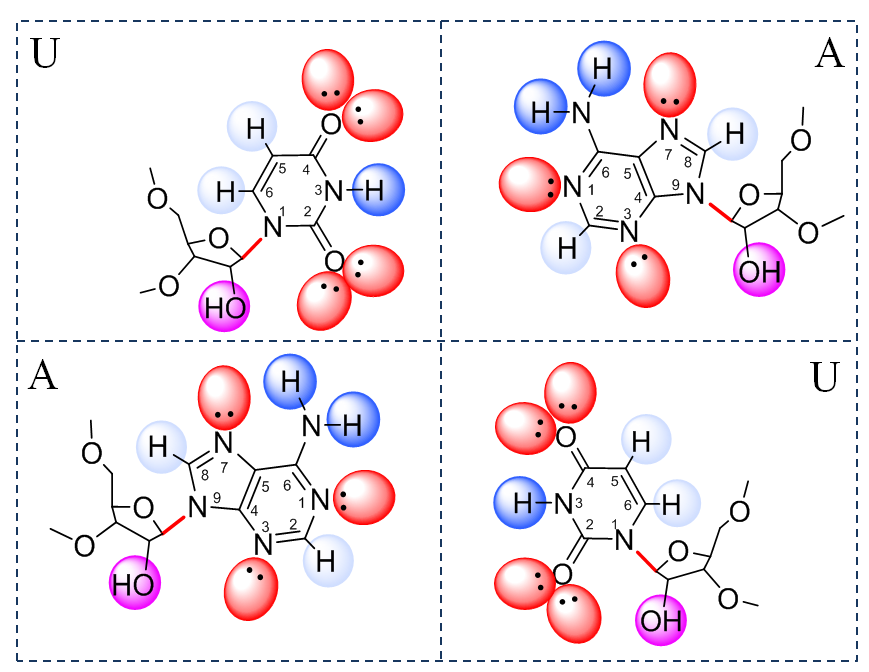
\includegraphics[width=\linewidth]{chapter-1/figs/ua}
  \caption{U and A Nucleotides to print on transparencies. U and A nts in two
    orientations to print on transparencies for making base pairs by juxtaposing
  H-bonding donor (blue) and acceptor (red) groups.}
\label{fig:ua}
\end{figure}

\begin{figure}
  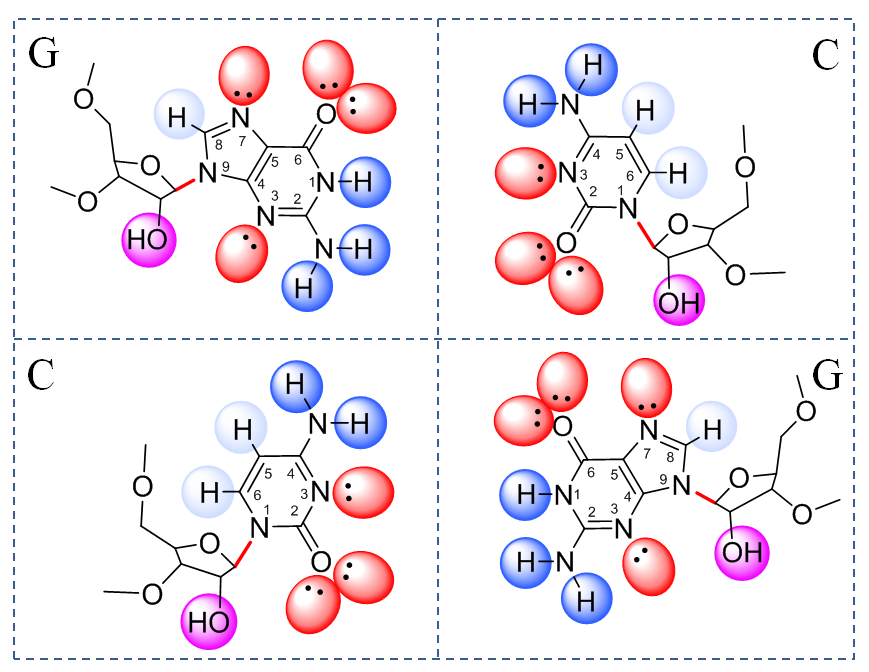
\includegraphics[width=\linewidth]{chapter-1/figs/gc}
  \caption{G and C Nucleotides to print on transparencies. U and A nts in two
    orientations to print on transparencies for making base pairs by juxtaposing
  H-bonding donor (blue) and acceptor (red) groups.}
\label{fig:gc}
\end{figure}

The H-bond acceptor groups are colored red in Figures~\ref{fig:ua}
and~\ref{fig:gc}, to reflect their overall negative charge. H-bond donor groups,
comprising H-atoms covalently bonded to electro-negative oxygen or nitrogen
atoms, are colored blue, reflecting their overall positive charges. The goal
when manipulating the colored transparencies is to obtain stable base pairs by
juxtaposing H-bond donors and acceptors so as to form at least two H-bonds. Each
red-colored functional group should partly overlap a blue-colored functional
group while avoiding any red-with-red or blue-with-blue juxtaposition. The 2’-OH
(hydroxyl) groups are colored purple to indicate that they can serve either as
H-bond donors or acceptors. Moreover, a single hydroxyl group can simultaneously
interact with an H-bond acceptor and at least one H-bond donor. The –OH bond can
rotate as needed to optimize H-bonding.

\begin{figure}
  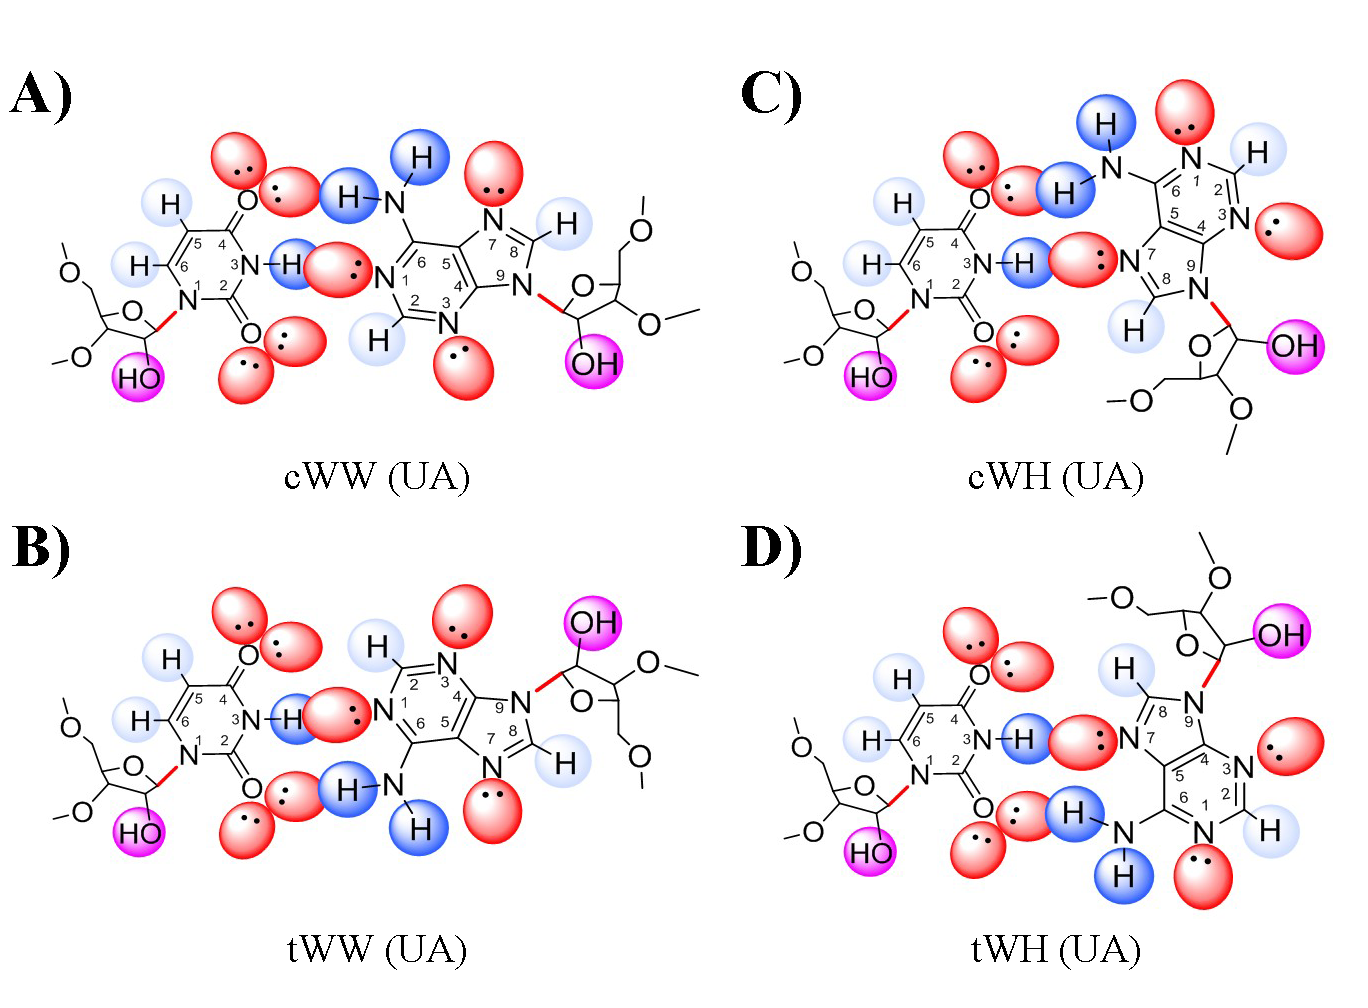
\includegraphics[width=\linewidth]{chapter-1/figs/basepairs}
  \caption{Representative basepairs. UA base combination in four different
    basepairing geometries: A. \emph{cis} Watson-Crick/Watson-Crick (cWW); B. \emph{trans}
    Watson-Crick/Watson-Crick (tWW); C. \emph{cis} Watson-Crick/Hoogsteen (cWH); and D.
  \emph{trans} Watson-Crick/ Hoogsteen (cWH).}
\label{fig:basepairs}
\end{figure}

To get started, readers can arrange the transparent cutouts of uracil and
adenine having WC edges facing in opposite directions to form the canonical AU
cis Watson-Crick (cWW) base pair. This pair is shown in Figure~\ref{fig:basepairs}A to illustrate
the complementary arrangements of color-coded H-bond donating and accepting
groups, red opposite blue. The H-atom attached to C2 of adenine (AH2) is colored
light blue to show that it is slightly polarized and capable of weak H-bonding
with O2 of uracil. Other H atoms covalently bonded to carbon atoms that are
sufficiently polarized to form weak H-bonds are also colored light blue. 

To form the non-WC trans Watson-Crick (tWW) UA pair, the A and U cutouts printed
with W edges facing in the same direction can be used.  Bringing together the W
edges forms an AU trans Watson-Crick (tWW) base pair, that can be compared with
Figure~\ref{fig:basepairs}B\@. This pair differs from the canonical (cis) Watson-Crick AU base pair
in the mutual orientation of the glycosidic bonds. In the cis pair, the
glycosidic bonds are on the same side of the base pair axis running through the
base centers parallel to the H-bonds, while in the trans pair, the glycosidic
bonds are on opposite sides of this axis.  

Next readers can reorient the W edge of the U so that it faces the H edge of the
A, juxtaposing complementary H-bond donor and acceptor groups. Results can be
compared with the pairs shown in Figure~\ref{fig:basepairs}
and~\ref{fig:basepairs}. There are two possible results, the \emph{cis} and the
\emph{trans} Watson-Crick/Hoogsteen pairings (cWH or tWH UA). These pairs are
stabilized by two strong H-bonds, involving NH donors, and one relatively weak
bond involving AH8. These base pairs have the same base combination (UA) as the
cWW and tWW pairs, but involve the Hoogsteen edge of A, illustrating that each
distinct combination of edges and glycosidic bond orientations produces a
different base-pairing geometry and therefore a different pair. 

Readers are encouraged to try other base combinations, to see how many form
stable pairs for each geometric family, and can check their base-pair models
against the on-line RNA Base pair Catalogue containing structures of all
observed and predicted base pairs organized by geometric family
(\URL{http://rna.bgsu.edu/FR3D/base pairs/}). The base combinations that form
pairs in each pairing geometry are summarized in Table~\ref{tab:base-combinations}.

\begin{landscape}
\begin{table}
  \begin{tabular}{lcccccccccccccccc}
    \toprule
        &              \multicolumn{4}{c}{A}             &             \multicolumn{4}{c}{C}          &               \multicolumn{4}{c}{G}       &            \multicolumn{4}{c}{U}            \\
    \cmidrule(r){2-5} \cmidrule(r){6-9} \cmidrule(r){10-13} \cmidrule(r){14-17}
        & A        & C        & G            & U         & A        & C        & G        & U         & A        & C        & G        & U        & A         & C        & G        & U          \\
    \midrule
    cWW & \I{1.4}  & \I{1.2a} & \I{1.3}      & \I{1.1}   & \I{1.2b} & \I{1.6}  & \I{1.1}  & \I{1.5}   & \I{1.3}  & \I{1.1}  &          & \I{1.2a} & \I{1.1}   & \I{1.5}  & \I{1.2b} & \I{1.7}    \\
    tWW & \I{2.7}  & \I{2.4}  &              & \I{2.2}   & \I{2.3}  & \I{2.9}  & \I{2.6}  & \I{2.8}   &          & \I{2.5}  & \I{2.7}  & \I{2.4}  & \I{2.1}   & \I{2.8}  & \I{2.3}  & \I{2.9}    \\
    cWH &          &          & \I{3.3}      & \I{(3.3)} &          & \I{3.2}  & \I{3.1}  & \I{(3.2)} & \I{3.3}  &          & \I{3.4}  &          & \I{(3.3)} &          & \I{3.1}  & \I{3.2}    \\
    tWH & \I{4.3}  &          & \I{4.3/4.2}  &           & \I{4.2}  & \I{4.1}  & \I{4.2}  &           &          &          & \I{4.5}  & \I{4.3}  & \I{4.1}   &          & \I{4.4}  & \I{4.2}    \\
    cWS & \I{5.1}  & \I{5.1}  & \I{5.1}      & \I{5.1}   & \I{5.2}  & \I{5.2}  & \I{5.2}  & \I{5.2}   & \I{5.3}  & \I{5.3}  & \I{5.5}  & \I{5.3}  & \I{5.4}   & \I{5.4}  & \I{5.4}  & \I{5.4}    \\
    tWS & \I{6.1}  & \I{6.2}  & \I{6.2}      & \I{6.1}   & \I{6.2}  & \I{6.1}  & \I{6.3}  & \I{(6.1)} &          & \I{6.3}  &          & \I{6.3}  & \I{6.3}   & \I{6.4}  & \I{6.4}  & \I{6.4}    \\
    cHH &          &          & \I{7.2}      &           &          &          & \I{7.1a} &           & \I{7.3}  & \I{7.1b} & \I{7.1}  &          &           &          &          &            \\
    tHH & \I{8.1}  & \I{8.1}  & \I{8.3}      & \I{8.3}   & \I{8.1}  &          & \I{8.1}  & \I{8.3}   & \I{8.2}  & \I{8.1}  & \I{8.4}  &          & \I{8.2}   & \I{8.2}  &          &            \\
    cHS & \I{9.1}  & \I{9.1}  & \I{9.1}      & \I{9.1}   & \I{9.1}  & \I{9.1}  & \I{9.2}  & \I{9.1}   & \I{9.1}  &          & \I{9.1}  &          & \I{9.3}   & \I{9.1}  & \I{9.1}  & \I{9.1}    \\
    tHS & \I{10.1} & \I{10.1} & \I{10.1}     & \I{10.1}  & \I{10.1} & \I{10.1} &          & \I{10.1}  &          &          & \I{10.2} &          & \I{10.2}  &          & \I{10.2} &            \\
    cSS & \I{11.1} & \I{11.1} & \I{11.1}     & \I{11.1}  & \I{11.1} & \I{11.1} & \I{11.1} & \I{11.1}  & \I{11.1} & \I{11.1} & \I{11.1} & \I{11.1} & \I{11.1}  & \I{11.1} & \I{11.1} & \I{(11.1)} \\
    tSS & \I{12.1} & \I{12.1} & \I{12.1}     & \I{12.1}  &          &          &          &           & \I{12.2} & \I{12.2} & \I{12.2} & \I{12.2} &           &          &          &            \\
    \bottomrule
  \end{tabular}
  \caption{Base combinations that form base pairs in each geometric family. The
    base combinations (columns) that form observed or predicted base pairs of
    the geometric type indicated in each row are marked with “x”. Base
    combinations that do not form base pairs are indicated by blank cells.
  [\URL{http://rna.bgsu.edu/FR3D/base pairs/BPfamilies.php}]}
\label{tab:base-combinations}
\end{table}
\end{landscape}

\subsubsection{The Sugar Edge}

A key concept for understanding sugar-edge base pairing is the role of the
ribose 2’-OH group, which can serve as an H-bond donor or acceptor, and often,
both simultaneously, on account of the free rotation of the hydroxyl group about
the C2’-O2’ single bond and the presence of the non-bonding electron orbitals on
the oxygen. Consequently, many different pairs can form using the sugar edges of
nts.  

\subsubsection{Protonation of the Watson-Crick edge of A and C}

Another important concept is that the imine nitrogen atoms, AN1 and CN3, on the
Watson-Crick edges of A and C, which are normally unprotonated and act as H-bond
acceptors, can be protonated at a modest energetic cost, when required by the
context, to convert these groups to H-bond donors. This allows certain base
combinations to form base pairs that cannot form when A or C are in their
unprotonated forms. Protonation confers a positive charge to the resulting BP,
which can help stabilize accumulations of negative charge, as occur, for example
in the close packing of phosphate groups or during chemical reactions
\cite{Siegfried2010, Cerrone-Szakal2008a}. Allowing for H-bonding to 2'-OH and
protonation of A and C Watson-Crick edges expands the number of base pairs one
can construct. 

\subsubsection{Specifying non-WC Base Pairs: Base combinations and Base-pair
families}

As readers experiment with the RNA base cut outs to construct base pairs, they
will quickly discover that the same base combination, for example UA in the
examples above, can form several different types of base pairs. To keep track of
the base pairs that form, readers should note the geometric base pair type or
family, in addition to the base combination. Giving the interacting edges of the
bases and the relative orientations, cis or trans, of the glycosidic bonds,
specifies the base pair family. To specify individual pairs, both the base
combination and the base pair family are needed, for example, UA tWH, UA cWW, or
CG cWW\@. 

It is necessary to specify the base combination because in each base pair
family, different base combinations (up to sixteen) can form the same type of
base pair. For example, fifteen of the sixteen base combinations, all except GG,
can form cWW base pairs. The base combination AG can form eleven of the twelve
different types of base pairs, all families except tWW\@. Referring to non-WC base
pairs as ``mismatches,'' as is frequently done in the literature, is imprecise and
misleading because for stable non-WC, as for WC, pairings, at least two H-bonds
form between the interacting edges. The only ``mismatches'' are those base
combinations that cannot form a particular base pair type. For example, GG is a
``mismatch'' for cWW but a stable ``match'' for tWW\@. It is better to simply speak of
``allowed'' and ``non-allowed'' base combinations for each base pairing geometry. As
noted above, some base combinations require protonation to form. In such cases,
the energy penalty for protonation is compensated by the more favorable binding
energy.

Readers can check their base-pair models against the on-line RNA Base pair
Catalogue containing structures of all observed and predicted base pairs
organized by geometric family (\URL{http://rna.bgsu.edu/FR3D/base pairs/}) and
by comparison with Table~\ref{tab:base-combinations}. The base combinations
(columns of Table~\ref{tab:base-combinations}) that form a stable pair in a
particular base pair geometry (rows of Table~\ref{tab:base-combinations}) are
indicated with an entry beginning with ``I.'' If no stable pair forms for that
geometry, the cell is left empty. Each column shows the base pair geometries
that each base combination can adopt. The 3D structures of base combinations
forming pairs in each geometric family can be viewed and downloaded as PDB files
from the pages of the online Base Pair Catalogue. 

Regarding Table~\ref{tab:base-combinations}, readers should note that for base pair geometries that
involve different edges (for example cWH or tHS) the order in which the bases
are listed makes a difference. For example, in the tWH AG base pair, the A
interacts with its W edge and the G with its H edge. Consequently, ``AG tWH''
and ``GA tWH'' refer to different base pairs. On the other hand, ``tWH AG'' and
``GA tHW'' refer to the same base pair. However, tHW pairs do not have their own
row in Table~\ref{tab:base-combinations} because they are redundant with tWH pairs. 

\subsection{Base pair Isostericity and Sequence Variation}

The classification of base pairs into geometric families based on edges provides
the framework for making sense of the base substitutions observed in structural
alignments of recurrent RNA 3D motifs and sequence alignments of RNA homologs
(for example, 16S rRNAs from different micro-organisms). To illustrate the basic
ideas, we first consider the AU, UA, GC, and CG Watson-Crick base pairs that
constitute the geometrically regular, anti-parallel double helices of RNA\@. RNA
helices are regular precisely because AU and GC pairs can substitute for each
other with little or no distortion of the helical geometry. They are said to be
isomorphic or “isosteric” to each other in the sense of occupying the same space
between the backbone atoms of the two strands of the helix. The property of
being isosteric can be quantified using a measure called the Iso-Discrepancy
Index (IDI), which depends on three distinct geometric features of base-pairs,
as illustrated in Figure~\ref{fig:idi}~\cite{Stombaugh2009}. The geometric
classification of base pairs is useful because only base pairs belonging to the
same family are isosteric by qualitative and quantitative (i.e.\ the IDI)
criteria. Isosteric pairs substitute for each other without distorting the local
RNA 3D structure. The IDI was calibrated by carrying out statistical analysis of
IDI values of isosteric and near isosteric AU, GC, and GU base pairs extracted
from high-quality structures. Quantitative analysis with IDI values confirms
that for two base pairs to be isosteric, they must belong to the same geometric
family~\cite{Stombaugh2009}. 

\begin{figure}
  \includegraphics[height=0.5\textheight]{chapter-1/figs/idi}
  \caption{Calculation of Iso-Discrepancy Index (IDI) to compare geometries of
    basepairs. The IDI is illustrated using non-isosteric base pairs. To
    calculate the IDI for two base pairs, the bases designated ‘first base’ in
    each base pair are superposed (bases on the left in each panel) and then the
    following three quantities are evaluated, normalized and summed: (1) The
    difference, ∆c, in the intra-base pair C1’–C1’ distances, illustrated for
    non-isosteric cWW AG and AU\@. (2) The inter-base pair C1’–C1’ distance, t1,
    between the C1’ atoms of the second bases of the base pairs, illustrated for
    the near isosteric cWW AU and AC base pairs. (3) The angle, theta, about an
    axis perpendicular to the base pair plane, required to superpose the second
  bases, illustrated using non-isosteric cWW AU and cWS AU base pairs.}
\label{fig:idi}
\end{figure}

All base pairs from the same geometric family have equal or very similar values
of the angle describing the mutual orientations of the glycosidic bonds of the
interacting bases, however they can differ by the other geometric measures used
to define the IDI (see Figure~\ref{fig:idi}). Therefore, not all base pairs belonging to
the same geometric family are necessarily isosteric. For example, purines and
pyrimidines differ considerably in size, so substituting a purine by a
pyrimidine or vice versa may change the space occupied by the base pair within
its structural context, as measured by the distance between C1' atoms of the
interacting nts. For example, substituting A for C in a cWW CG base pair to
produce cWW AG significantly increases the C1'-C1' distance from \TILDE 10.4 \AA,
typical for AU or GC, to \TILDE 12.3 \AA\@. Consequently, this substitution distorts the
helix and destabilizes neighboring base pairs in the helix. Consistent with this
prediction, substitution of base combinations AG or GA for cWW CG or AU pairs
within regular helices of homologous RNA molecules is rare, and cWW AG pairs
occur almost exclusively on the ends of helices, often adjacent to junction
motifs where they provide a large surface for stabilizing inter-helix stacking
interactions~\cite{Sponer2003}. An example is the cWW AG pair, found in most
tRNAs at the top of the anticodon stem-loop and flanking the tRNAs MHJ
\cite{Romby1985}.

To properly align the H-bond donor and acceptor groups of the substituted bases,
it may be necessary to shift the bases laterally relative to the positions of
the original bases. Such a shift is needed when U substitutes for C to transform
a GC to a GU cWW pair, so that the H-bond donor and acceptor groups on the
Watson-Crick edges of G and U can align. The U shifts laterally toward the major
(deep) groove, relative to the G, to form the GU pair. This geometric change is
not as disruptive to adjacent base pairs, as the changes in C1'-C1' distances
that occur with AG cWW pairs. Consequently, GU pairs are observed quite
frequently within Watson-Crick helices in RNA molecules. The cWW GU pair is
considered ``near isosteric'' to cWW GC and AU\@. However, the lateral shift breaks
the symmetry of the cWW geometry, so cWW GU and UG pairs are geometrically
distinct and not isosteric or even near isosteric to each other. In each base
pair family, different sets of base combinations form pairs that are isosteric
to each other. For example, the base combinations AG and CU are isosteric in the
tHS family although they are not isosteric in the cWW family~\cite{Leontis2002f, Leontis1998b}.

These considerations predict that those base substitutions that result in
isosteric or near isosteric base pairs should be much more likely to occur
between homologous molecules than non-isosteric ones. The rRNAs of \EC{} and
\TT{} provide an ideal, large-scale test case for this hypothesis, because these
two bacteria are phylogenetically and ecologically divergent. Nonetheless, their
3D rRNA structures are sufficiently conserved that a large percentage of base
pairs in the two structures can be structurally aligned and compared
\cite{Stombaugh2009}. The base pairs of 5S, 16S, and 23S rRNAs from high quality
structures of 70S ribosomes of these species were aligned manually to identify
corresponding base pairs. It was found that over 90\% of base pairs could be
aligned and analyzed using the IDI\@. This analysis showed that 72\% of
corresponding base pairs in the 5S, 16S, and 23S rRNAs of \EC{} and \TT{} were
isosteric and unchanged in sequence, 19\% were isosteric and different in
sequence, 7\% were near isosteric, and only 2\% were non-isosteric
\cite{Stombaugh2009}. In total, almost 98\% of the alignable base pairs in the
two structures were isosteric or near isosteric. This results provides strong
support for the generalization that base substitutions in homologous RNA
molecules or recurrent structural motifs are constrained to preserve isosteric
base pairings, whether the pairings are WC or non-WC.

NDB provides annotations for base pairs and other nt interactions for all
atomic-resolution 3D structures [9]. The annotations are accessible from the
main page of each structure. 

\subsection{Base Triples}

Base triples are common sub-motifs in RNA 3D motifs. All base triples can be
decomposed into combinations of base pairs, in which a central base is paired to
each of the other two bases of the triple using a different base edge. All in
all there are 108 different geometric base triple families of which 68 have been
observed in experimental structures~\cite{AbuAlmakarem2012b}. The base-pair
families to which a base triple's component base pairs belong define the base
triple family to which it belongs. A catalog of observed base triples can be
accessed online through NDB\@. New base triples can be found by symbolic search
using FR3D~\cite{Petrov2011a}. 

\subsection{Base-Stacking Interactions}

The energetically most stabilizing contributions to RNA structure are provided
by the hydrophobic van der Waals forces mediating stacking of the faces of RNA
bases on each other~\cite{Sponer2010}. Because RNA bases lack rotational
symmetry, the two faces are not equivalent. Therefore two RNA bases can stack
face-to-face in four distinct ways, depending on which base faces come into
contact. The faces are distinguished by reference to the orientation of each
base in the Watson–Crick helix, in which all bases are in the anti-glycosidic
conformation; the ``5′-face'' points toward the 5′-end of the strand and the
``3′-face'' points toward the 3′-end of the strand~\cite{Hoehndorf2011,
Sarver2008a}. A systematic analysis of the sequence propensities of base
stacking in all possible geometries and contexts is still lacking. NDB provides
base-stacking annotations for all RNA structures which can be used as a basis
for such studies. 

\subsection{Base-backbone Interactions }

\subsubsection{BPh interactions}

As each nt bears a full negative electrical charge, RNA molecules need to
overcome electrostatic self-repulsion to achieve compact folding. The negative
charge of each nucleotide is largely concentrated on the two non-bridging oxygen
atoms of the phosphate groups, resulting in electrostatic repulsion between
phosphate groups but enhancement of H-bonding to donors on base edges of the RNA
bases.  The stabilizing H-bonding interactions between bases and the phosphate
backbone moieties, referred to as ``base-phosphate'' (BPh) interactions, help to
reduce intra-molecular repulsion between phosphate groups while specifically
stabilizing compactly folded structural motifs and architectures. The
classification of BPh interactions by base is shown in Figure 14. This
classification is the result of structural bioinformatics study combined with
quantum mechanical (QM) calculations and molecular dynamics simulation studies
\cite{Zirbel2009, Zgarbova2011a}. The QM calculations revealed the optimal
geometries and the intrinsic stabilizing energies of these interactions, and
showed that the most stable BPh interactions, those on the W edge of G, rival GC
WC base pairs in stability. Very stable BPh interactions also are formed by the
WC edge of U and the Hoogsteen edge of C (see Figure~\ref{fig:bph} and citation
\cite{Zirbel2009}).

\begin{figure}
  \includegraphics[width=\textwidth]{chapter-1/figs/bph}
  \caption{Base-Phosphate (BPh) interactions observed in RNA 3D structures for
    each base. H-bonds are indicated with dashed lines. BPh categories are
    numbered 0–9, starting at the H6 (pyrimidine) or H8 (purine) base positions.
    BPh interactions that involve equivalent functional groups on different
    bases are grouped together: 0BPh (A, C, G, U), 5BPh (G, U), 6BPh (A, C),
    7BPh (A, C) and 9BPh (C, U). Bridging interactions, 8BPh and 4BPh, are
  especially stable.}
\label{fig:bph}
\end{figure}

Many recurrent 3D motifs contain specific BPh interactions that tend to be
highly conserved. For instance, many hairpin loops, including the anti-codon and
T-loops of tRNAs, contain the ‘U-turn' submotif, a sharp bend in the backbone
stabilized by H-bonding between the WC edge of U and the phosphate of the N+3
base of the loop~\cite{Quigley1976} A conserved BPh interaction involving the
conserved ``bulged'' G is observed in recurrent sarcin-ricin (S/R) internal loop
motifs~\cite{Correll1998}. Conserved GU wobble base pairs are observed to bind
anionic oxygen phosphate atoms in the minor groove to facilitate tight packing
of helical elements~\cite{Mokdad2006b}. It is necessary to consider conserved
BPh interactions to fully account for the chemical protections observed in 16S
rRNA~\cite{Merryman1999, Stern1988}. These examples show that BPh interactions
are widespread in RNA structures and play significant roles in RNA folding, as
documented in Table~\ref{tab:helix-loop-inter}.

\subsubsection{Base-Ribose Interactions}

The 2'-OH of ribose participates in sugar-edge base pairs, acting as both H-bond
donor and acceptor. It is considered part of the nt Sugar edge. H-bonds can also
form with the ribose O4' atom, acting as H-bond donor. Another type of
interaction involves stacking of bases on ribose rings as shown in
Figure~\ref{fig:base-ribose}. The example in this figure is a key interaction
that stabilizes the binding of tRNAs to the P-site of the 30S subunit. The
base-ribose stacking occurs between the ribose of the first anti-codon nt of
tRNA (G34) in the anti-codon HL (nts 32--38 of tRNA) and the highly conserved
base G966, located in HL 34 of 16S rRNA (an intermolecular loop-loop
interaction). Because only the tRNA ribose and not the base is involved in the
interaction with 16S, the base can vary in sequence, allowing tRNAs with
different anti-codon sequences to bind to the same site. The 16S base involved
in the interaction, G966, on the other hand is highly conserved and is in fact
chemically modified~\cite{Burakovsky2012}. The sequence propensities of
base-ribose stacking interactions also deserve attention. Annotations of
base-ribose interactions are also posted on NDB\@.

\begin{figure}
  \includegraphics[width=\textwidth]{chapter-1/figs/base-ribose}
  \caption{Base-ribose stacking interaction. The conserved base-ribose stacking
    interaction involving ribose 34 in the anti-codon of tRNA bound to the
    P-site of 16S rRNA and conserved base G966 in 16S\@.  From PDB file
    4GD1~\cite{Dunkle2011a}.}
\label{fig:base-ribose}
\end{figure}

\subsubsection{Metal-ion mediated phosphate-phosphate interactions}

Structured RNA molecules generally require multi-valent metal ions to fold into
their compact, functional structures~\cite{Woodson2005, Bowman2012, Draper2005,
Draper2013, Auffinger2011, Tan2011}. This is because cations like \ce{Mg2+} can
bridge between two or more negatively charged phosphate groups, allowing compact
structures to form in which phosphate groups are in close proximity. Cationic
polyamines and basic proteins can also promote RNA folding~\cite{Klein2004a,
Koculi2006}. \ce{Mg2+} is particularly well suited to facilitate rRNA compaction
because it is abundant in cells and has a very high charge density among
biologically available ions, owing to its relatively small ionic radius (0.6\AA)
and +2 electrical charge. \ce{Mg2+} associates preferentially with the anionic
non-bridging oxygen atoms of the phosphate groups. 

\subsection{RNA 3D motifs and non-WC pairs}

Recurrent modular 3D motifs generally correspond to individual HL, IL, or MHJ
loops. As we have seen, ``loops'' play very important roles in structured RNA
molecules. While some motifs appear to be unique, many occur over and over in
unrelated RNA molecules. Most recurrent 3D motifs are relatively small (less
than \TILDE 20 nts) and therefore can evolve independently in unrelated
molecules. For example, kink-turns, sarcin-ricin motifs, C-loops, and GNRA or
UNCG HL are found in many different molecules and even in multiple locations in
the same large RNA molecule. In fact, 16S rRNA contains instances of each of
these motifs. Non-WC pairs play two fundamental roles in RNA 3D structure: (1)
They are the building blocks of RNA 3D motifs~\cite{Leontis2006}, where they
provide the specific local interactions that structure individual HL, IL and MHJ
3D motifs. (2) Non-WC pairs mediate most LR (tertiary) interactions, usually in
combination with LR WC pairs, base-stacking, and base-phosphate interactions, as
discussed above for 16S rRNA\@. As we have seen, most of these interactions occur
between loop nts or loop and helix nts. The different types of non-WC pairs tend
to contribute to different extents to local vs.\ LR interactions, as shown in
Table~\ref{tab:bp-family-counts}. For example, cWW, tWH, and tHS together
account for almost 90\% of local base pairs, whereas cSS, tSS, cWS, tWS and cWH
account for almost 80\% of long-range (LR) pairs. 

\begin{table}
  \begin{tabulary}{\linewidth}{LRRRRRR}
    \toprule
                    & \multicolumn{2}{c}{Local Interactions} & \multicolumn{2}{c}{Long-range Interactions} & \multicolumn{2}{c}{All Interactions} \\
    \cmidrule(r){2-3} \cmidrule(r){4-5} \cmidrule(r){6-7}
    Basepair Family & Counts & Frequency (\%) & Counts & Frequency (\%) & Counts & Frequency (\%) \\
    \midrule
    cWW    & 460    & 75.3                     & 12     & 15.6                     & 472    & 68.6                     \\
    tWW    & 9      & 1.5                      & 2      & 2.6                      & 11     & 1.6                      \\
    cWH    & 8      & 1.3                      & 5      & 6.5                      & 13     & 1.9                      \\
    tWH    & 37     & 6.1                      & 1      & 1.3                      & 38     & 5.5                      \\
    cWS    & 9      & 1.5                      & 4      & 5.2                      & 13     & 1.9                      \\
    tWS    & 7      & 1.1                      & 5      & 6.5                      & 12     & 1.7                      \\
    cHH    & 0      & 0.0                      & 0      & 0.0                      & 0      & 0.0                      \\
    tHH    & 3      & 0.5                      & 0      & 0.0                      & 3      & 0.4                      \\
    cHS    & 11     & 1.8                      & 0      & 0.0                      & 11     & 1.6                      \\
    tHS    & 41     & 6.7                      & 2      & 2.6                      & 43     & 6.3                      \\
    cSS    & 12     & 2.0                      & 30     & 39.0                     & 42     & 6.1                      \\
    tSS    & 14     & 2.3                      & 16     & 20.8                     & 30     & 4.4                      \\
    Totals &        & 100\%                    &        & 100\%                    &        & 100\%                    \\
    \bottomrule
  \end{tabulary}
  \caption{Local vs.\ Long-range Interactions in \EC{} 16S rRNA by Base-pair
  Family.}
\label{tab:bp-family-counts}
\end{table}

Use of the base-pair symbols shown in Table~\ref{tab:bp-families} to annotate local interactions
that structure HL, IL, and MHJ captures much of the crucial information found in
the 3D structure. An example of a recurrent 3D motif from 16S rRNA is the
internal loop of helix 20 which is a variant of bacterial loop E of 5S rRNA
\cite{Leontis1998a}. Renditions of the 3D and annotated 2D structures are shown
in Figure~\ref{fig:compare-il}A and B. The \EC{} and \TT{} versions of this
recurrent motif are superposable in 3D space even though the sequences are
different because corresponding bases form isosteric base pairs of the same
geometric type, as shown in Figure~\ref{fig:compare-il}B \& C. This and several
related 3D motifs were predicted from sequence analysis based on non-WC base
variations observed in sequence alignments, before the release of the
atomic-resolution 3D structures of the 16S rRNAs~\cite{Leontis1998,
Leontis2002e}. This example illustrates the general principle that corresponding
motifs in homologous RNA molecules often fold into very similar 3D structures
and are stabilized by the same interactions, that is the same types of base
pairs, stacking and BPh interactions~\cite{Petrov2013}.

\begin{figure}
  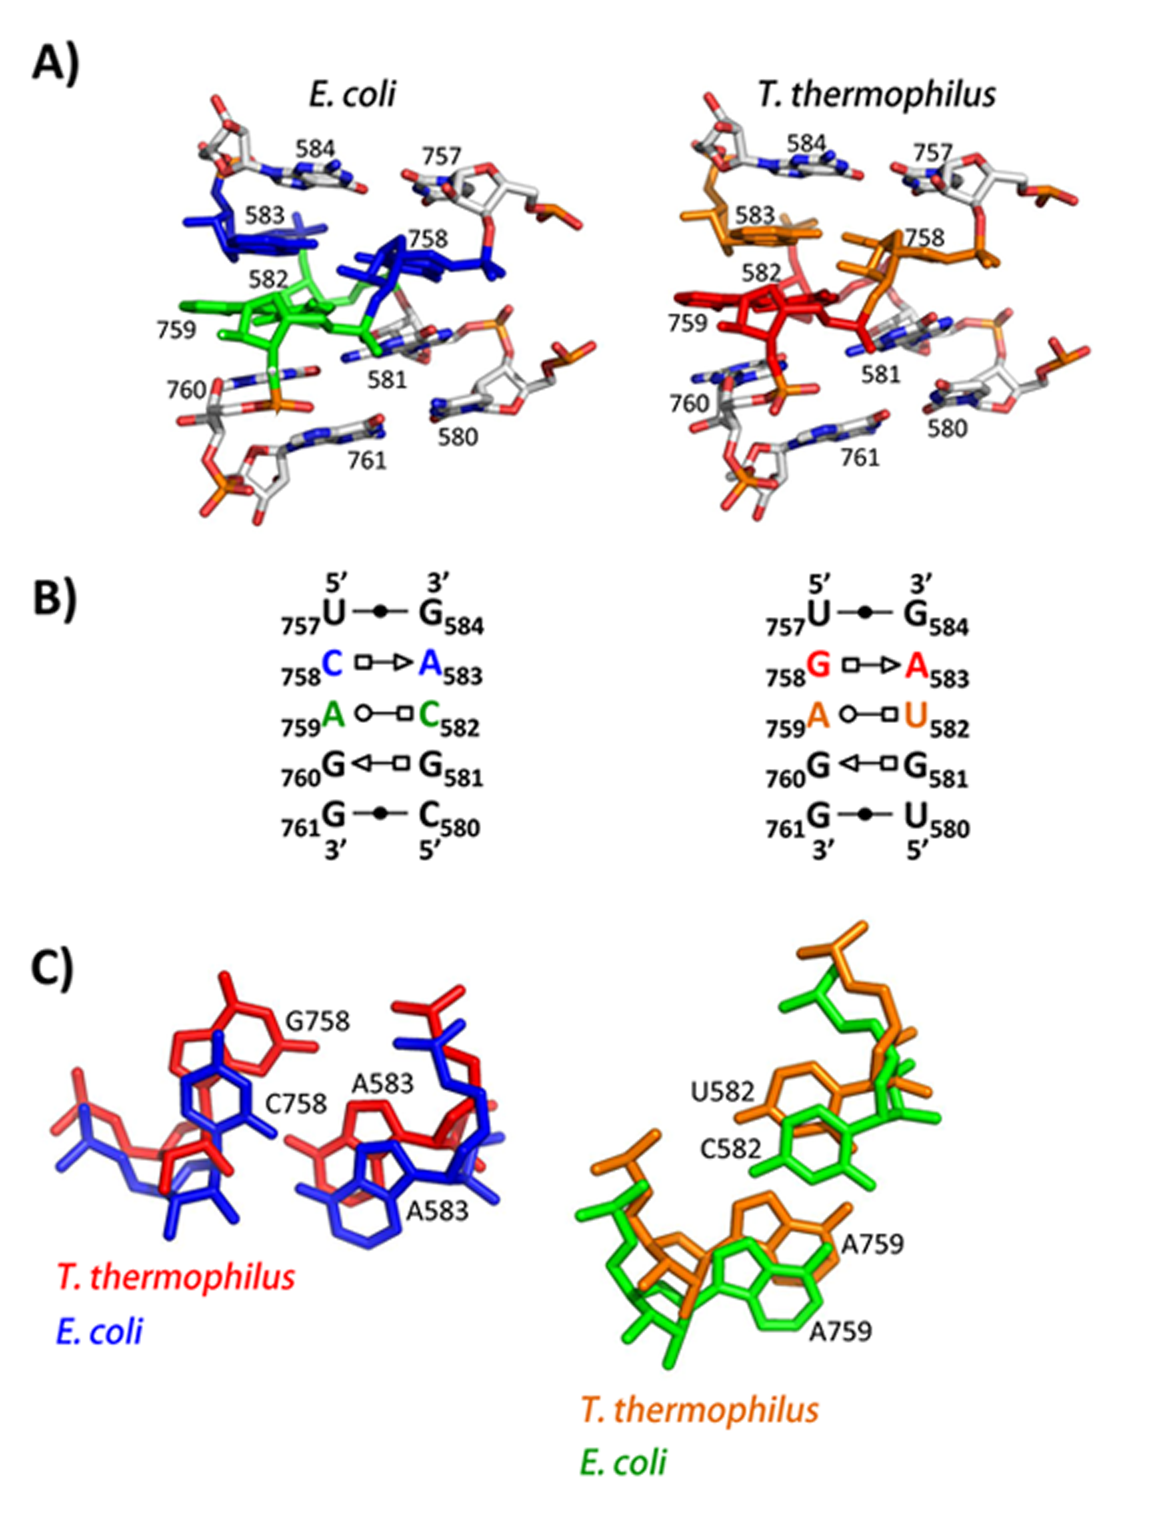
\includegraphics[width=0.5\textwidth]{chapter-1/figs/IL-20}
        \caption{A. 3D structures of IL from helix 20 of 16S rRNA (PDB files
        2AW7~\cite{Schuwirth2005} and 1FJG~\cite{Carter2000}). B. 2D annotations
        showing conserved non-WC basepairs. Although they differ in sequence,
        the two motifs have the same interactions
    and are assigned to the same motif group. C. Superposition of isosteric tWH
    and tSH non-Watson-Crick basepairs from the \EC{} and \TT{} versions of the
    helix 20 motif.}
\label{fig:compare-il}
\end{figure}

Grouping structurally similar RNA motif instances in motif families and aligning
corresponding nts among them is crucial to improving bioinformatic methods for
RNA 3D structure prediction based on sequence. In addition to variations in
sequence, recurrent, structurally similar motifs can also differ in the number
of nts they comprise. A key question is which motifs to group together.
Structural analysis based on conserved nt interactions suggests that when the
extra nts found in the larger motifs are bulged out so as not to interact with
the core nts of the motif, and the corresponding core nts form identical
interactions, then the motifs should be assigned to the same group. For example,
some GNRA-type HL have five nts instead of four, but the additional nt is bulged
out without affecting the conformations of the other nts~\cite{Nasalean2009b}.
Similarly, there is considerable variation in the number of nts in kink-turn and
C-loop IL motifs, but this variation is largely confined to the looped out nts
on one strand~\cite{Lescoute2005}.

\section{Resources for Exploring RNA 3D Structures}

\subsection{RNA 3D Motif Atlas}

These observations provide a framework for classifying recurrent 3D RNA motifs
by geometric similarity. Motifs are assigned to the same motif groups when
corresponding nts form the same interactions, regardless of motif size. This
approach was found to be more successful than relying exclusively on root-mean
square deviations (rmsd) of atomic coordinates and was implemented to construct
the RNA 3D Motif Atlas, a continuously updated resource~\cite{Petrov2013}. The
Motif Atlas features automatic extraction of 3D motifs (HL and IL) from the
current non-redundant (NR) dataset of RNA-containing of NDB files and clustering
into structurally similar motifs~\cite{Petrov2013}. The Motif Atlas is
comprehensive and representative and can be accessed through NDB or directly at
\URL{http://rna.bgsu.edu/rna3dhub/motifs}.

\subsection{Nucleic Acid Database (NDB)}

The NDB (\URL{http://ndbserver.rutgers.edu}) is a web portal providing access to
information about 3D nucleic acid structures and their complexes. In addition to
primary data that is archived in PDB, the NDB contains derived geometric data,
classifications of structures and motifs, standards for describing nucleic acid
features, and tools and software for analyzing DNA and RNA\@. A variety of
search capabilities are available, as are many different types of reports. The
NDB was recently redesigned and continues to evolve to meet the changing needs
of RNA scientists. NDB provides sophisticated search capabilities at the level
of whole structures by a large number of criteria. With the growth of interest
in RNA biology and chemistry, the NDB is offering new RNA-derived data and
annotations and integrating them into the search
capabilities~\cite{CoimbatoreNarayanan2014}. For example, NDB is developing
finer-grained search capabilities at the level of individual motifs and
interactions. NDB also provides curated descriptions and links to useful tools
and software for RNA scientists (readers should visit
\URL{http://ndbserver.rutgers.edu/ndbmodule/services/softwares.html}).

\subsection{Automated annotation of nt interactions in RNA 3D Structures}

Atomic-resolution 3D structures reveal the architectures of RNA molecules and
the stabilizing local and LR nt interactions. However RNA 3D structures are
complex and difficult for students and non-specialists to comprehend and
interpret. Identifying and classifying individual nt interactions is tedious and
error-prone work when done manually. It is for this reason that computer
programs have been written by several different research groups to automate and
standardize this process~\cite{Petrov2011a, Sarver2008a, Yang2003a,
Gendron2001b, Parisien2008a}. The different programs produce annotations that
largely agree with each other; discrepancies occur mainly when annotating
low-resolution structures that are poorly modeled. Annotations of most of the
recurrent nt interactions discussed here are now made available for each new
atomic-resolution experimental RNA 3D structure when it appears in NDB
\cite{Petrov2013}. Annotations are accessible under ``Structural Features'' in
the upper left of each structure summary page of NDB\@. 

\subsection{Integrating 2D and 3D RNA structural representations}

RNA 2D diagrams illustrate at a glance the folding of the chain to form the
nested Watson-Crick paired helices, identify the domain structure of the RNA and
the sizes and positions of individual HL, IL, and MHJ loops. They can provide
road maps for accessing the 3D structures because it is so easy to find
individual nts in the 2D and to identify neighboring nts in the same helical
elements and loops. What the 2D lacks, of course, are the local and LR non-WC
pairing, stacking and backbone interactions and the spatial relationships
between helical elements. However, interactive computer technology can fill the
gap between the over-simplification of 2D diagrams and the complexity of the 3D\@. 

The most basic step is the use of color to coordinate the 2D and 3D
representations of RNA molecules, as illustrated for 16S in
Figure~\ref{fig:ec-ssu-2d-3d}. Nts belonging to the same helical element are
colored in 3D as shown in the 2D\@. Coordinated color-coding of 2D and 3D
structures by helical element facilitates identifying the elements to which
interacting nts belong. In the 3D structure, helical elements distant in the 2D
can be in close proximity and each helical element can interact with several
different elements, not to mention proteins and ligands.  We have provided
SwissPDBViewer and PyMol files with these color codings as supplementary files
to this article to allow readers to visualize \EC{} 16S rRNA on their own
computers. 

The 2D can also be used to rapidly access specific regions of the 3D structure.
In this approach clickable ``hotspots'' are embedded at the locations of
structural features on the online 2D diagram, for example all HL and IL of the
molecule. Clicking on the hotspots brings up an interactive window in which the
3D structure of the selected motif is displayed. Links can be provided to the
motif family to which the motif belongs to access sequence variants of the
motif. One can access 2D diagrams of representative 16S and 23S rRNA molecule
that feature this capability at this link:
\URL{http://rna.bgsu.edu/rna3dhub/motifs/2ds}.

While it is possible to represent all local and LR base pairs on a static 2D
representation, the resulting ``circuit diagram'' is difficult to interpret and
comprehend~\cite{Lescoute2006a}. An alternative approach is to equip interactive
2D diagrams with sets of controls to selectively display different classes of
interaction by type or location. A prototype of such a display for 16S rRNA can
be accessed here \URL{http://rna.bgsu.edu/rna3dhub/pdb/2AW7/2d}.

\subsection{From 1D to 2D to 3D RNA structures}

It will never be possible to solve the 3D structures of all the RNAs we find in
nature at atomic resolution. Fortunately, it may not be necessary to do so as
bioinformatic tools have been developed and are under constant improvement to
predict 2D and 3D RNA structures starting from individual sequences or
alignments of homologous RNA molecules~\cite{Leontis2012e}. 

The first step is to predict the 2D structure to identify the helical regions
and define the nts that belong to HL, IL, MJ or linker segments. Dynamic
programming algorithms that make use of a growing database of nearest neighbor
thermodynamic parameters have been refined to make this step quite reliable,
especially when chemical probing or complementary phylogenetic data are
available, i.e.\ sufficiently diverged homologous sequences~\cite{Aigner2012}.
The most commonly used resources are listed in the table provided in
supplemental materials. 

The next step in structure prediction is to identify recurrent HL, IL or MHJ
motifs based on loop sequences identified in the 2D or to carry on de novo
modeling based on energy parameters. Many groups are developing de novo modeling
tools~\cite{Rother2012a, Sijenyi2012, Flores2012, Ding2012a, Cao2012}. ``RNA
Puzzles'' has been established to provide CASP-like blind tests of these tools,
leading to rapid progress in RNA 3D modeling~\cite{Cruz2012}. Accessible through
NDB is JAR3D, a new on-line tool that is closely linked to the 3D Motif Atlas.
This tool matches user-provided sequences for HL or IL to the most probable
matches of motifs found in the Motif Atlas using observed sequence variations
and considerations of isosteric base pairs to score sequences (see
\URL{http://rna.bgsu.edu/main/webapps/jar3d/}).

The next step once the 2D structure is determined and possible 3D structures of
HL and IL are proposed is to predict the conformations of MHJs
\cite{Lamiable2012, Laing2011}.This step is crucial as the MHJ determine the
relative orientations of helical elements in 3D space. It is computationally
challenging. Improvements in the prediction of MHJ in 2D structures also
continue to be made~\cite{Liu2011b}.

The final step is to predict tertiary interactions between loops and helical
elements that stabilize the 3D architecture. This step is also very challenging
but is greatly facilitated by sequence analysis when sufficiently diverged and
properly aligned homologs are available for analysis~\cite{Michel2000,
Westhof2011}.

\subsection{Conclusion}

We have illustrated, using 16S rRNA, the prevalence of loop nts in structured
RNAs and their central roles in mediating local and long-range interactions that
stabilize the 3D architecture and make possible the specific binding of
proteins, ligands, and other RNA molecules. We have provided a tutorial to
familiarize readers with the most sequence specific of those interactions, the
WC and non-WC base pairs, and showed that by grouping them in geometrically
similar families and isosteric groups, it is possible to interpret and even
predict the sequence variations of recurrent RNA 3D motifs. The distinction
between base combination and base pair geometry was emphasized, because the same
combinations of bases (e.g. UA, AG, CC) can make different types of base pairs.
Base substitutions that preserve the base-pairing geometries maintain functional
structures and are more likely to occur. Annotating interactions is a
prerequisite for grouping 3D motifs into structurally similar groups. This is
how the Motif Atlas is organized. As the number of sequence variants for known
motifs increases, that information can be automatically incorporated to improve
algorithms to predict RNA 3D structure. 

Finally we have provided links to resources to allow readers to deepen their
understanding of RNA 3D structure and access specific information about RNAs of
interest to them. New ways of integrating 2D and 3D representations of
structured RNAs will make it easier for students and scientists to explore and
comprehend the structures, functions, and evolution of these amazing, ancient
molecules. New bioinformatic tools will make it possible to evermore reliably
predict the 2D and 3D structures and possible functions and interactions of new
RNA molecules.

\chapter{OVERVIEW OF THE RNA.BGSU.EDU DATA PIPELINE, DATABASE AND SUPPORTED
ON-LINE RESOURCES}

In this chapter I will discuss the \href{http://rna.bgsu.edu}{RNA.BGSU.EDU}
pipeline and database. The aim is provide the reader with an overview of the
pipeline and familiarity with concepts and design. This chapter will first
provide a context for my work on the pipeline by discussing the goals, rationale
for this work and the principles defining the design of the pipeline and
database. This will then discuss the scientific value of our pipeline followed
by the design and how it allows us to achieve the principles. Finally we will
provide an overview of the implementation. 

\section{Goals for the BGSU RNA pipeline}

One of the major grant activities in our lab is the development, maintenance and
extension of our data pipeline and database that imports data from new
RNA-containing structure files as they appear in PDB on a weekly basis. The
pipeline is a python and Matlab application that annotates all pairwise
nucleotide interactions, groups structurally similar RNA molecules into
equivalence sets, identifies high quality representative sets of RNA structures
and extracts and clusters RNA 3D motifs and stores all these derived data in a
locally maintained MySQL database.

We have developed these tools to achieve the aims of NIH founded work carried
out in collaboration with with Dr. John Westbrook and Dr. Helen Berman at the
Nucleic Acids Database (NDB). This is the sixth year of the collaboration, which
began in 2010. The aims of the grant are:

\begin{enumerate}
        \item Deepen our understanding of RNA 3D structure by extracting and
                organizing 3D motifs

        \item Improve our understanding of the structure variation of RNA
                molecules and RNA complexes by examining and comparing 3D
                structures assigned to the same sequence/structure "equivalence"
                class.

        \item Accelerate the study of the correspondence between RNA 3D
                structure and RNA sequence

        \item Provide annotations for RNA-protein interactions

        \item Develop new and extended tools for delivery, search and
                visualization of the RNA sequence and structure annotations
                described in Aims 1-4 and make them available in the NDB.
\end{enumerate}

As a part of the grant we provide annotations to NDB on a weekly basis. These
data include our nonredundant sets and associated equivalence sets, nucleotide
interaction annotations, as well as motif clusterings. In the near future we
will add RNA-protein interactions.

The data computed in our pipeline are used to support research resources. We
provide the RNA community with the BGSU RNA site, the RNA 3D motif library,
JAR3D, WebFR3D, R3DAlign, and R3D-2-MSA. As these resources require access to
up-to-date RNA structures, it is essential that the database and pipeline always
produce all the required data.

Secondly, it is essential that the pipeline be easy to maintain, extend and
improve by successive groups of graduate students and research associates. After
the departure of Anton Petrov and during most of my Ph.D. work it has been my
responsibility to maintain and update the pipeline and database. During the time
I was charged with these responsibilities major improvements were made to take
advantage of new mmCIF formats from PDB. The following projects are underway
that will extend the pipeline's capabilities: 
\begin{enumerate*}
        \item Poorna Roy is writing code to annotate nucleotide-amino acid
                interactions, 
        \item Maryam Husseieni is writing code to annotate and extract
                multi-helix functions and cluster them for the RNA 3D Motif
                Atlas, 
        \item Once finalized these results will be written into the database 
        \item We continue on an ongoing basis to improve base-pair annotation
                (Dr. Craig Zirbel), loop extraction (my work) and motif
                clustering.
\end{enumerate*} 
As soon as these new results and functions are tested and validated these
improvements will be integrated into the pipeline's weekly update functions.

Thus the operations goals for our database and pipeline are:
\begin{enumerate}
        \item The pipeline must store only correct data in the database
        \item The pipeline must run reliable each week to maintain current data
        \item The pipeline must be ease to maintain, update and improve
\end{enumerate}

In the next sections I will discuss how the changes I have made to the previous
version help us achieve these goals.

\section{Comparison of the current BGSU RNA pipeline to other resources}

We have evaluated other software options and found them unsuitable for our
current aims. The main resource we considered was the previous implementation by
Dr. Anton Petrov \cite{Petrov2012}. The implementation was a part of his dissertation research.
Much of the previous pipeline was not suitable for our current requirements.

First, the previous version did not work with mmCIF data. In December 2014, the
protein databank (PDB) transitioned from the outdated fixed columnar width  PDB
format to a new mmCIF format for all 3D structure data.

Second, the previous version of the database and pipeline did not work to ensure
the validity of data. Consequently, I discoverd that our database contained
"orphan data". Orphan data is data that is missing related information. For
example, there were structures which had been placed into an NR group, but we
had no information on the resolution. In addition, a careful reading of the code
showed it was possible for the pipeline to write incomplete data. Incomplete
data is when we do not write all annotations for a structure. For example, if
there are 100 annotated base pairs, writing 99 of them would constituent writing
incomplete data. My rewrite was aimed at fixing these issues as well as
usability of the pipeline.

Finally, the previous version did not centralize the core logic of the pipeline
in a module making the pipeline harder to maintain. To explain, all parts of the
pipeline have the same core logic as detailed in a later section. Each part of
the pipeline that computes data is referred to as a ``stage''. The stage is
primarily responsible for computing data, while the core manages ensuring that
the overall pipeline behaves correctly.

A good example of centralizing logic, is the logic for rolling back failed
imports and checking if data has been computed. The previous version had not
centralized this logic so adding new computations required the programmer to add
logic to ensure that these actions happened correctly. In addition, requests to
remote resources were not always retried leading to some requests being more
fragile than others.

Another potential option was to use is the
\href{https://github.com/pharmbio/sciluigi}{sciluigi} which is built off the
luigi package provided by Spotify. Sciluigi package contains a framework for
building pipelines and is being adopted by the bioinformatic community. I have
chosen not to use sciluigi because it was released after I had already written a
large portion of the pipeline. While sciluigi is a well designed framework it
does not offer a compelling reason to rewrite large portions of our existing
framework. Had it existed prior to my start I would have likely used it.

\section{Design requirements for the BGSU RNA pipeline and database}

In more detail, to support the research goals, our pipeline must fulfill the
following requirements.

\begin{enumerate}
        \item The pipeline must always keep the database in a valid state.
        \item The pipeline must operate efficiently and avoid recomputing data unnecessarily
        \item The pipeline should facilitate user control when manual operation is required.
        \item The pipeline must be as reliable as possible.
        \item The pipeline must be designed so additions will respect all constraints.
\end{enumerate}

We will discuss each requirement and the rationale behind each one.

\subsection{Maintaining validity of data}

For a database to remain valid, two properties must be maintained. First, the
database must be complete. This means that the database should not be left in a
state with any partial data for any structure. For example, the database should
not have partial base pair annotations for a given structure: it should have all
or none. This requirement must be respected because our data supports several
sources: equivalence classes of similar structures and the representatives sets
they support and the annotations we provided to NDB
\cite{CoimbatoreNarayanan2014}, also the R3D-2-MSA \cite{Cannone2015}, JAR3D
\cite{Roll2016}, WebFR3D \cite{Petrov2011a}, and R3DAlign \cite{Rahrig2013}
sites all rely on data produced by pipeline in the database.

\subsection{Ensuring the validity of the database}

The second property of a valid database is that it is consistent. Consistency is
best explained through an example. Keeping the database consistent means
preventing situations from arising where we annotate a base pair involving RNA
nucleotide residues that we have not yet created and stored in the database. In
database terms, this requirement is referred to as preventing "orphan data".
Whenever data are inconsistent any analysis or display of the stored data will
fail, for lack of referenent.

By striving to keep the database in a valid and consistent state, we ensure that
the database is always usable for analysis and display on webpages, even when
the pipeline fails to update with new data. Without this it would make our other
tools, such as JAR3D and RNA 3D Hub, unstable. Providing these resources in an
ongoing and stable manner is a major grant activity in the lab, which is why
this is the most important design consideration of the pipeline.

Preventing the writing of incomplete or orphan data is also essential to
avoiding or minimizing the unnecessary recomputation of data. As we learned
during the transition of CIF format files, which required the computation of
most annotations, recomping all data for each each run of the pipeline would
take several weeks. This is too slow and completely unnecessary for our planned
weekly update runs of the pipeline. Thus the pipeline is designed to only
compute data for new structures or manually specified structures that need to be
recomputed for some particular reason, at the manager's discretion.

\subsection{Controlling the pipeline}

The next priority, ease of controlling which stages and structures to run during
manual operation, is intended to facilitate error correction. Work with previous
version of the pipeline showed that extensive manual work was always needed to
rerun the correct stages with the correct data. This manual work was
error-prone, and frequently produced even more problems that need correction. By
automating the repetitive manual work, I succeeded in making it easier to
recover from errors.

\subsection{Pipeline Reliability}

The fourth consideration is that the pipeline must be as reliable as possible.
Reliability means that the pipeline will compute as much data as possible
despite errors. Errors in programs are inevitable and must be anticipated in the
design of the pipeline. Even if all parts of the pipeline are written correctly
it can still fail because of anomalous events generated by external resources.
For example, the pipeline has failed when:  PDB provided incomplete data or when
the network experienced instability during few fractions of a second required to
complete a web request. These and other issues that I have encountered during
the years I was responsible for pipeline operation, convinced me of the high
priority of making the pipeline as robust as possible.

The final consideration is ease of adding new "stages" to provide new
functionality as this will carried out on an ongoing basis by current and new
students involved in the project. They should be able to make changes without
having to know all the details of how the pipeline works, confident that they do
not have to deal with ensuring the validity of the database and the stability of
the pipeline in order to make improvements and additions of new functionality.

\section{Implementation of the BGSU RNA data pipeline}

In this section I discuss the improvements to the pipeline that enable it to
fulfill the design requirements outlined above. These improvements required
coordinated changes to occur both in the pipeline application and the database.
Each requirement in turn.

\subsection{Ensuring data validity}

To maintain validity of data in a database, it is essential to add constraints
to the database. Constraints are requirements on one or more columns that ensure
certain criteria must be met before adding or modifying data in that column. The
constraints I have added include uniqueness constraints and foreign key
constraints as appropriate. Constraints were added to  nearly every table in the
database. These constraints could not be added prior to these improvements
because the database was not configured to allow them.

A uniqueness constraint ensures that no two rows in the same table may have the
same data values in any column. Uniqueness constraints may span more than one
column. For example, I have added a uniqueness constraint on the ``pdb\_id'' and
``chain\_name'' column in the ``chain\_info" table. This table stores information
about all chains and by placing the uniqueness constraint on these two columns I
ensure that there can be no two chains in the same structure with the same
combination of PDB id and chain name. This constraint reflects the logical
structure of the data. By adding these constraints, I ensure that the data in
the database is logically correct as regarding chains.

The second type of constraint I introduced is the consistent implementation of
foreign keys wherever required to allow the many tables in our database to work
together properly. These ensure that entries in one column of one table exist in
another column of another table. These safeguard data completeness. The use of
foreign keys allows the expression of the requirement of ``interactions must be
built from known residues'. To describe a specific example, we have a table
called ``unit\_info'' which contains data for all residues, RNA, DNA, protein,
ligands, etc, known in the database. In the unit\_info table there is a
``unit\_id'' column that provides a unique identifier for all units (i.e.
residues, whether RNA, DNA or protein). The ``unit\_pairs\_interactions'' table
contains all pairwise interactions between RNA residues, such as base pair and
base stacking interactions. It contains a ``unit\_id\_1'' and ``unit\_id\_2'' column
which specify the first and second units forming the interaction. For an
interaction represented by a row in the unit\_pairs\_interactions table to be
valid, the entries in the ``unit\_id\_1'' and ``unit\_id\_2'' must exist  in the
``unit\_id'' column of the ``unit\_info'' table. I have enforced this logical
requirement by declaring that ``unit\_id\_1'' and ``unit\_id\_2'' are foreign keys
link to ``unit\_id'' in the unit\_info table.

At the level of the pipeline application, I ensure data validity by implementing
procedures to automatically rollback failed imports. Because we have foreign key
and uniqueness constraints, it is possible to attempt to write data that will be
rejected. For example, if the pipeline attempts to write an interaction between
units that do not exist, the database will reject the data because of the
foreign key constraints. I rewrote the pipeline so that in the event of such an
error during a data entry operation, all interactions that were written for that
structure will be deleted. This prevents the writing of partial data for any
single structure, ensuring the database remains complete, ie ensuring the
absence of partial data.

\subsection{Minimizing the number of computations}

If the pipeline were to recompute all data on every update a single run would
take at least several weeks to complete with currently available resources.
Given that we are committed to provide weekly updates to NDB, this is
unacceptable. However, the capability to easily force data to be recomputed is
also crucial. For example, we update our classification of pairing interactions
from time to time. When this is done, we must be able to easily update the
entire database with the new pairing annotations. I have implemented the
capability to make such updates by simply telling the pipeline to delete the old
data and recompute the new data.

I have changed the pipeline execution to first check whether data have already
been computed for each input and only computing data when none are present, or
when the user explicitly requests the pipeline to select recompute selected
data. Now as currently configured all parts of the pipeline go through the steps
shown in Figure~\ref{fig:stage-flow}. With this logic I can ensure that only the
required data are computed. The previous version of the pipeline had a similar
capability however my additions make it more comprehensive, as well as, ensuring
that old data are always deleted prior to recomputing existing data. In the
previous version it was not required that all parts have consistent behavior in
the face of existing data. I have centralized the logic for recomputing and
deleting old data.

\begin{figure}
  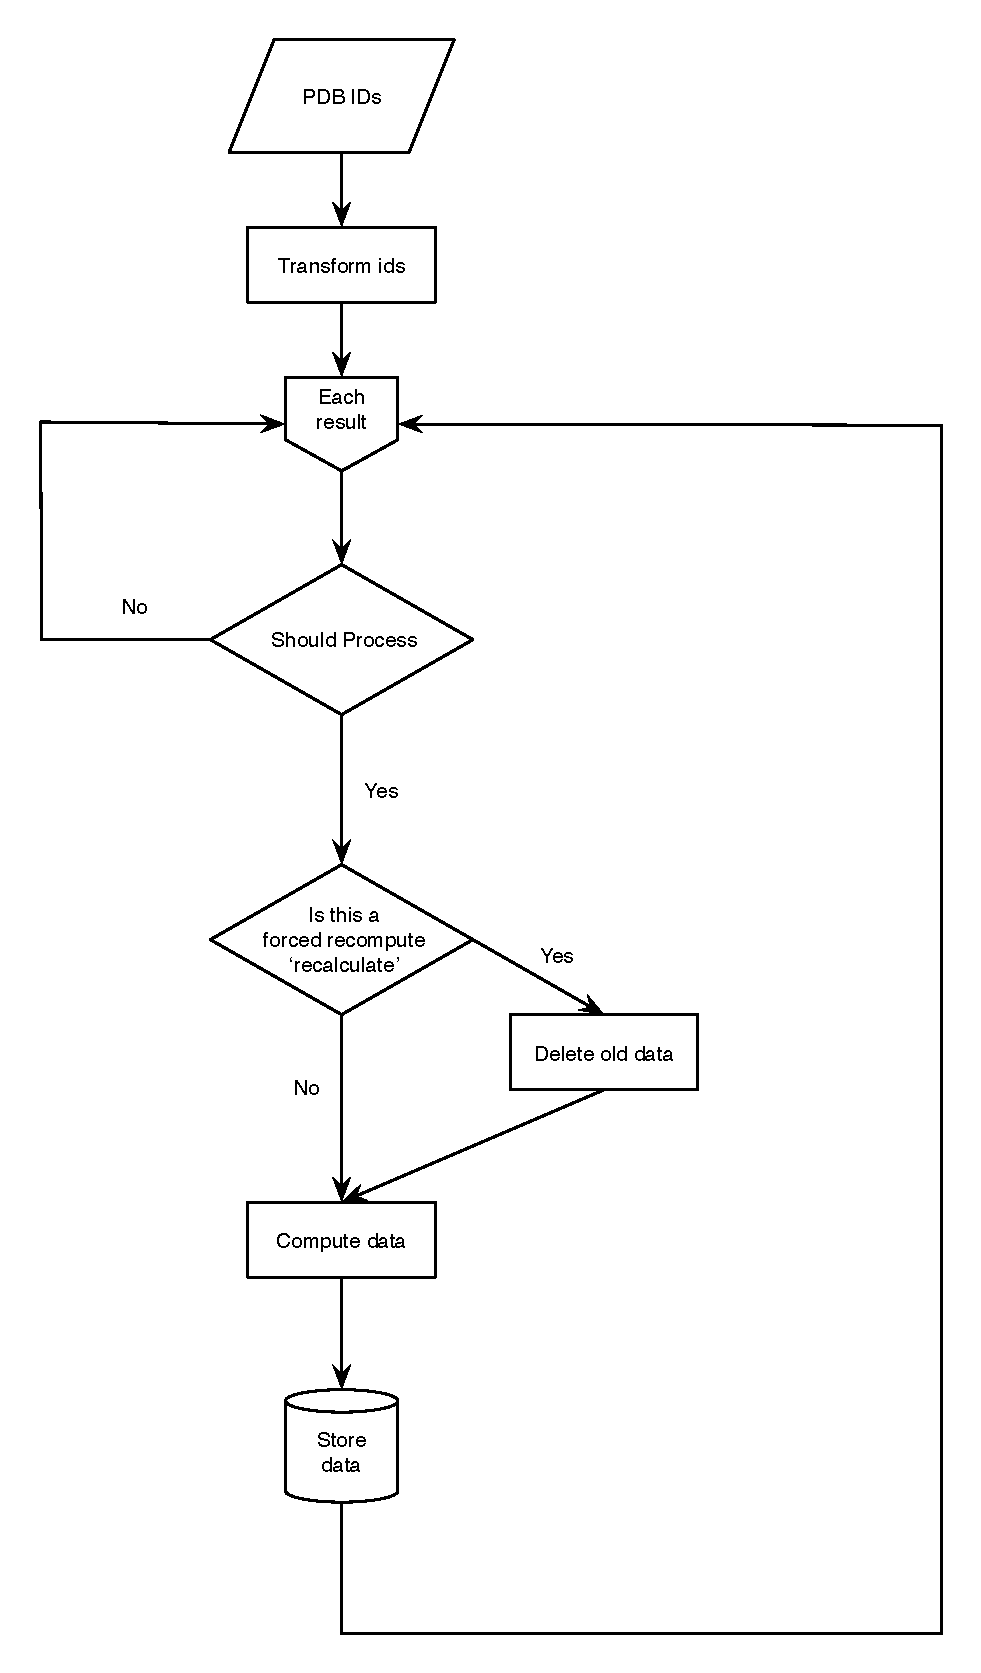
\includegraphics[height=8in]{chapter-2/figs/stage-flow}
\caption{Figure summarizing the logical flow for each stage. This figure shows
the general scheme of all stages.}
\label{fig:stage-flow}
\end{figure}

This requirement ensures efficient execution times of our pipeline. Without it
our weekly, or even monthly update schedule could not be maintained. However, in
order to correctly skip recomputing old data, the database must always be
complete. Should the pipeline begin to save incomplete data, it will never
attempt to recompute and fill in missing data. For this reason, it is essential
that the database always remain complete.

\subsection{Providing control over the data computed}

The day-to-day goal of the pipeline is to run weekly updates using all available
structures. In this case the intent is to compute all annotations for all
structures. However, it is often useful and sometimes necessary to run specific
annotations on specific structures. For example, when testing a new set of
annotations it is desirable to select a few test structures on which to run only
the new annotations, and then examine the results.

To make this possible, I have restructured the pipeline to provide a single
unified point of entry that takes as input the name of the part to run and the
particular structures to analyze, or an option to include all available
structures. In the previous version of the pipeline there were several possible
entry points. The primary entry point was the ``update'' component. This part
would run everything required for a weekly update in the correct order. The
other entry points were specific to individual components such as loading
interactions. This was an issue because parts of the pipeline have dependencies
upon each other. For example, to compute the pairwise interactions, the
structure must first be downloaded. Previously, these dependencies were implicit
in the design of the update component and were not stated explicitly, leading to
potential confusion.

These dependencies are now encoded into the pipeline using a dependency graph as
shown in Figure~\ref{fig:stage-deps}. This graph can be sorted using a topological
sort to produce a linear ordering. I have implemented this logic as part of the
``dispatcher'' which determines which modules to run and in which order to run
them in for a given application.


\begin{figure}
  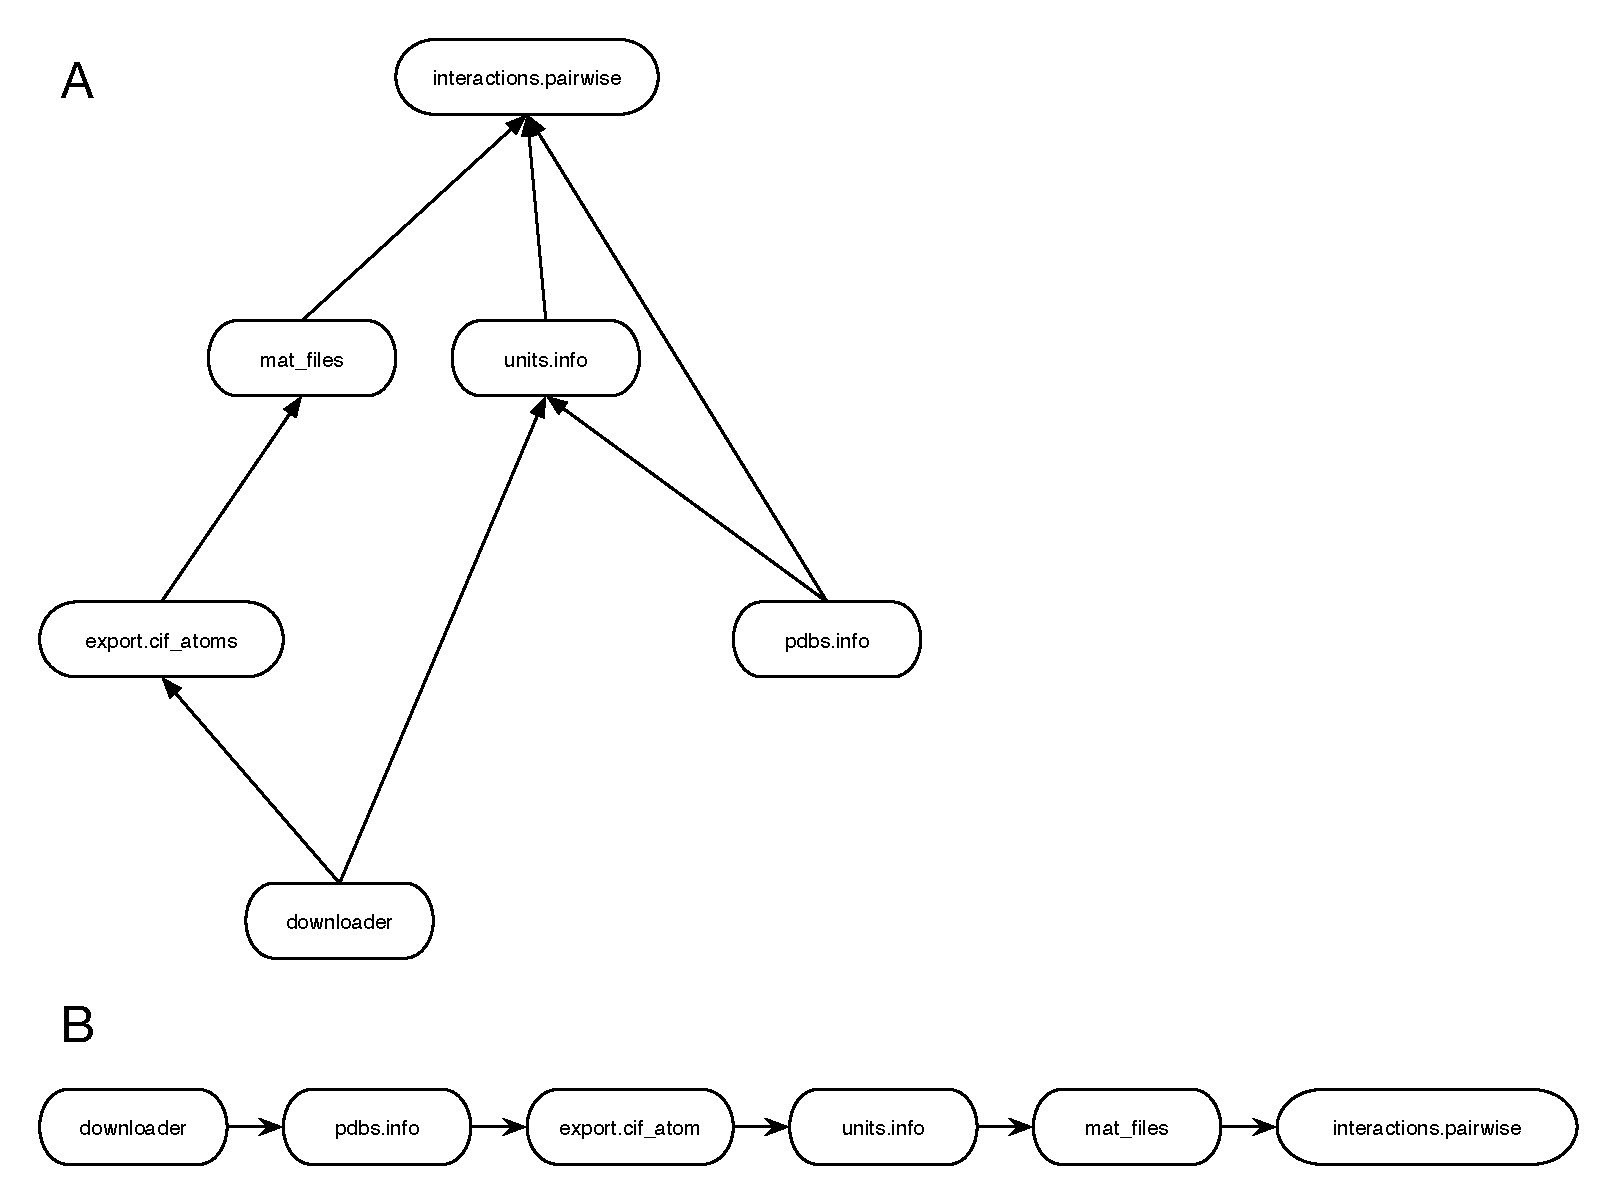
\includegraphics[width=\linewidth]{chapter-2/figs/deps}
  \caption{An example of an unsorted dependency graph (top) and a topological
    sorted dependency graph (bottom). Each stage is represented by an oval with
    the name of the stage in the oval. In this case the user has requested that
    the ``interactions.pairwise'' stage is run. This stage depends on two other
    stages, ``mat\_files'' and ``units.info'' as shown by the connections to those
    stages. Those stages have further dependencies. Shown in the bottom is the
    result of topological sorting the stages.}
\label{fig:stage-deps}
\end{figure}

With dependencies encoded in the pipeline, operators of the pipeline can request
the pipeline run a set of stages at once. In addition, part of the input to the
pipeline may optionally specify which dependencies do not need to be run. This
allows for the expression of complex requirements like, ``rerun all unit level
annotations except the distance and coordinate computation'. This is often
useful when testing out new parts or after fixing failed runs. When running all
structures, simply checking which input needs to be processed can take several
hours for some stages. When fixing a failed run or testing a new annotation, the
programmer will often already know which stages have been run. By instructing
the pipeline to run only those stages that are needed the overall run time can
be decreased.

With the previous version, to accomplish something similar to this it was
necessary to edit the code each time. I did this on several occasions and found
that it was very possible to forget that some parts were edited, since
computations could take hours, and in doing so left the code in a bad state for
the next weekly update. Because some parts were edited we did not run a complete
pipeline, leading to unexpected failures. This was then fixed by undoing the
edits that I previously made. Providing the capability to the pipeline operator
to what to run we avoid this problem entirely.

In addition, the main entry point now accepts either a list of PDB structures to
process or options to fetch the structures to run. The options and their usage
is explained in more detail in the ``Operation of the pipeline'' section. The
previous version always used all structures by default. While this is typically
the case, there are many situations where the operator wants to alter the
operation of the pipeline. For example, if one structure was not correctly
imported, only the failed structure should be rerun. By allowing the user to
select the structures specifically we make the pipeline easier to control.The
default mode of operation nonetheless remains. I have also added options to
allow selection of all structures that were available as of a specified date, or
prior to the current one. This has proven extremely useful when computing in old
releases during the update.

Operation of the the pipeline has been facilitated by implementing a single
entry point that takes as in input specifications for those parts parts to be
run and structures to be used. This ease of use also makes the pipeline more
reliable as it is no longer necessary to alter code to customize pipeline
operation.

\subsection{Making the pipeline robust to failures}

The pipeline will inevitably encounter errors during its operation. A robust
pipeline is one that gracefully fail. These errors can result from many sources.
The most obvious are mistakes in the code itself, for example, the pipeline may
have a bug in new code that causes it to attempts to for example, write invalid
quality data (a new feature). The second are errors introduced by external
resources. Part of our weekly update procedure is to fetch the list of all files
that are available as of the current date. This request to PDB can fail, because
all networks subject to intermittent failure. The final type of error is
mistakes in the input we are processing. For example, mmCIF files have certain
assumptions about their structure. In the past, some mmCIF files have not
respected their own assumptions leading to errors arising in the pipeline.I have
encountered all three types of errors and have worked to make the pipeline
robust in the face of these issues as discussed in the next paragraphs.

For the first set of errors, bugs in the code itself, I have added extensive
error handling code. The handling covers all aspects of the computing of and
saving of data to the database. Error handling identifies when errors occur and
alerts the user to the cause. Combined with extensive logging his aids in
debugging. The pipeline can cleanup, as required for validity, as well as
attempt to continue with other inputs. In addition, because the pipeline assumes
each input to a stage is independent and thus does not fail right away. This
leads the pipeline to attempting to compute data for all inputs to a stage prior
to failing. This provides a robustness against failures for specific inputs.

The next set of possible errors are those due to external resources. An example
of this type of work is fetching the quality report for a structure. PDB
provides quality data for all structures on their FTP site, which the pipeline
fetches for import. These requests can fail because of an unstable network.
However, these network errors are transient. The best way to handle network
errors is by identifying them as such and resubmitting the request.

I have modified the pipeline to retry requests to all external resources. Since
any request may fail due to network errors, the pipeline is now programmed to
always retry when a network error is encountered. It will retry up to the
specified number of attempts before failing. This allows for the pipeline to
deal with intermittent network failures, but not persistent failures. Longer
term issues such as a complete failure of the network will still cause the
pipeline to fail. However, this is acceptable since the pipeline could not
compute the required data. In addition, the requests can validate their
response. This helps with dealing in errors that happen when external sites
claim they sent data but the pipeline receives no data. For example, in the past
when querying PDB's services to attain the list of all files, PDB's response was
empty. This is not true as at the time about 2000 files were available, however
due to some error in their services we received a response stating there files
available.

The final type of issue, mistakes in the input data, does not have a simple
solution. Throughout the code, I have added checks to ensure the data is valid.
This allows confidence that the data being computed is correct. However, there
is no general purpose reusable way to always check that the mmCIF file is
formatted correctly. In addition we cannot simply retry computations as the data
will still be formatted incorrectly leading to the same errors. I dealt with the
issue mentioned above, a mmCIF violating its own design assumptions with
additions to the mmCIF reader to deal with this specific issue. I have added
extensive logging to the pipeline so that when this type of issues arises again
it will be flagged.

\subsection{Ease of extension}

The pipeline must be easy to extend. In order to make this possible I have
centralized all the essential logic of the pipeline into a few core classes that
can be inherited when creating a new stage. A class according to wikipedia is
"an extensible program-code-template for creating objects, providing initial
values for state (member variables) and implementations of behavior (member
functions or methods" (CITE
https://en.wikipedia.org/wiki/Class\_(computer\_programming)). Python, which the
pipeline is mostly written in, is an object-oriented language and users
interested in working with it are strongly recommended to study the language.
The majority of the pipeline is written using an intermediate or beginner level
of python. None of the advanced features, metaclasses for example, are used. I
will attempt to explain some fundamentals of python and object-oriented
programming here.

Classes can ``inherit'' behaviors from other classes. This is commonly done
through ``inheritance'. Inheritance is a common feature of object oriented
programming where in there is a base class or parent which defines some
functionality. From there one or more classes ``inherit'' the functionality and
are called ``child'' classes. This relationship forms a hierarchy of classes. The
behavior of any class is defined by the code in the class and all parent
classes. The child class can then extend the parent class functionality by
adding new behaviors. In addition, the child may override the parent class
behaviors by providing it's own implementation of specific behaviors. The child
implementation of any behavior is always prefered over the parent behavior.

In the pipeline there is a parent class that defines the overall stage flow
shown in Figure~\ref{fig:stage-flow}. Users can add a  new stages, called the
``child'' class, which ``inherit'' from this parent class and receives all the
standard behaviors such as deleting failed imports and only recomputing when
needed. A user may decide that some stage should never delete data in the case
of a failed import. For example, our loop ids are meant to never change and
allowing automatic deletion may cause issues. Thus if we want to be safe the
class that implements the logic of importing loops overrides the deleting
behavior to do nothing except log an error.

Because classes inherit the essential functionality of the pipeline, new users will only have to
implement 1) the logic for querying the database to see if this structure has already been
processed and 2) the logic to create the data to store.
Operation of the pipeline
In this section, I discuss the RNA.BGSU.EDU pipeline at a high level, to familiarize readers with
its functionality, organization, operation and documentation. Salient details will be provided,and
complete references will be provided to direct readers to the relevant sections of the detailed
documentation. We begin with an overview of the structure of the code and of the application,
followed by configuration options, and end with directions for running the pipeline.

\section{Execution of the pipeline}

The pipeline is a Python and matlab application that is publically accessible at
\href{https://github.com/BGSU-RNA/RNA-3D-Hub-core}. Detailed documentation is
available for the python code at \href{http://rna-3d-hub-core.readthedocs.io/}.
Our relational database is MySQL and the schema is not currently public.

The application is organized into a series of directories, as shown in
Figure~\ref{fig:pipeline-organization}. This figure displays the key directories
and explains their contents.

\begin{figure}
  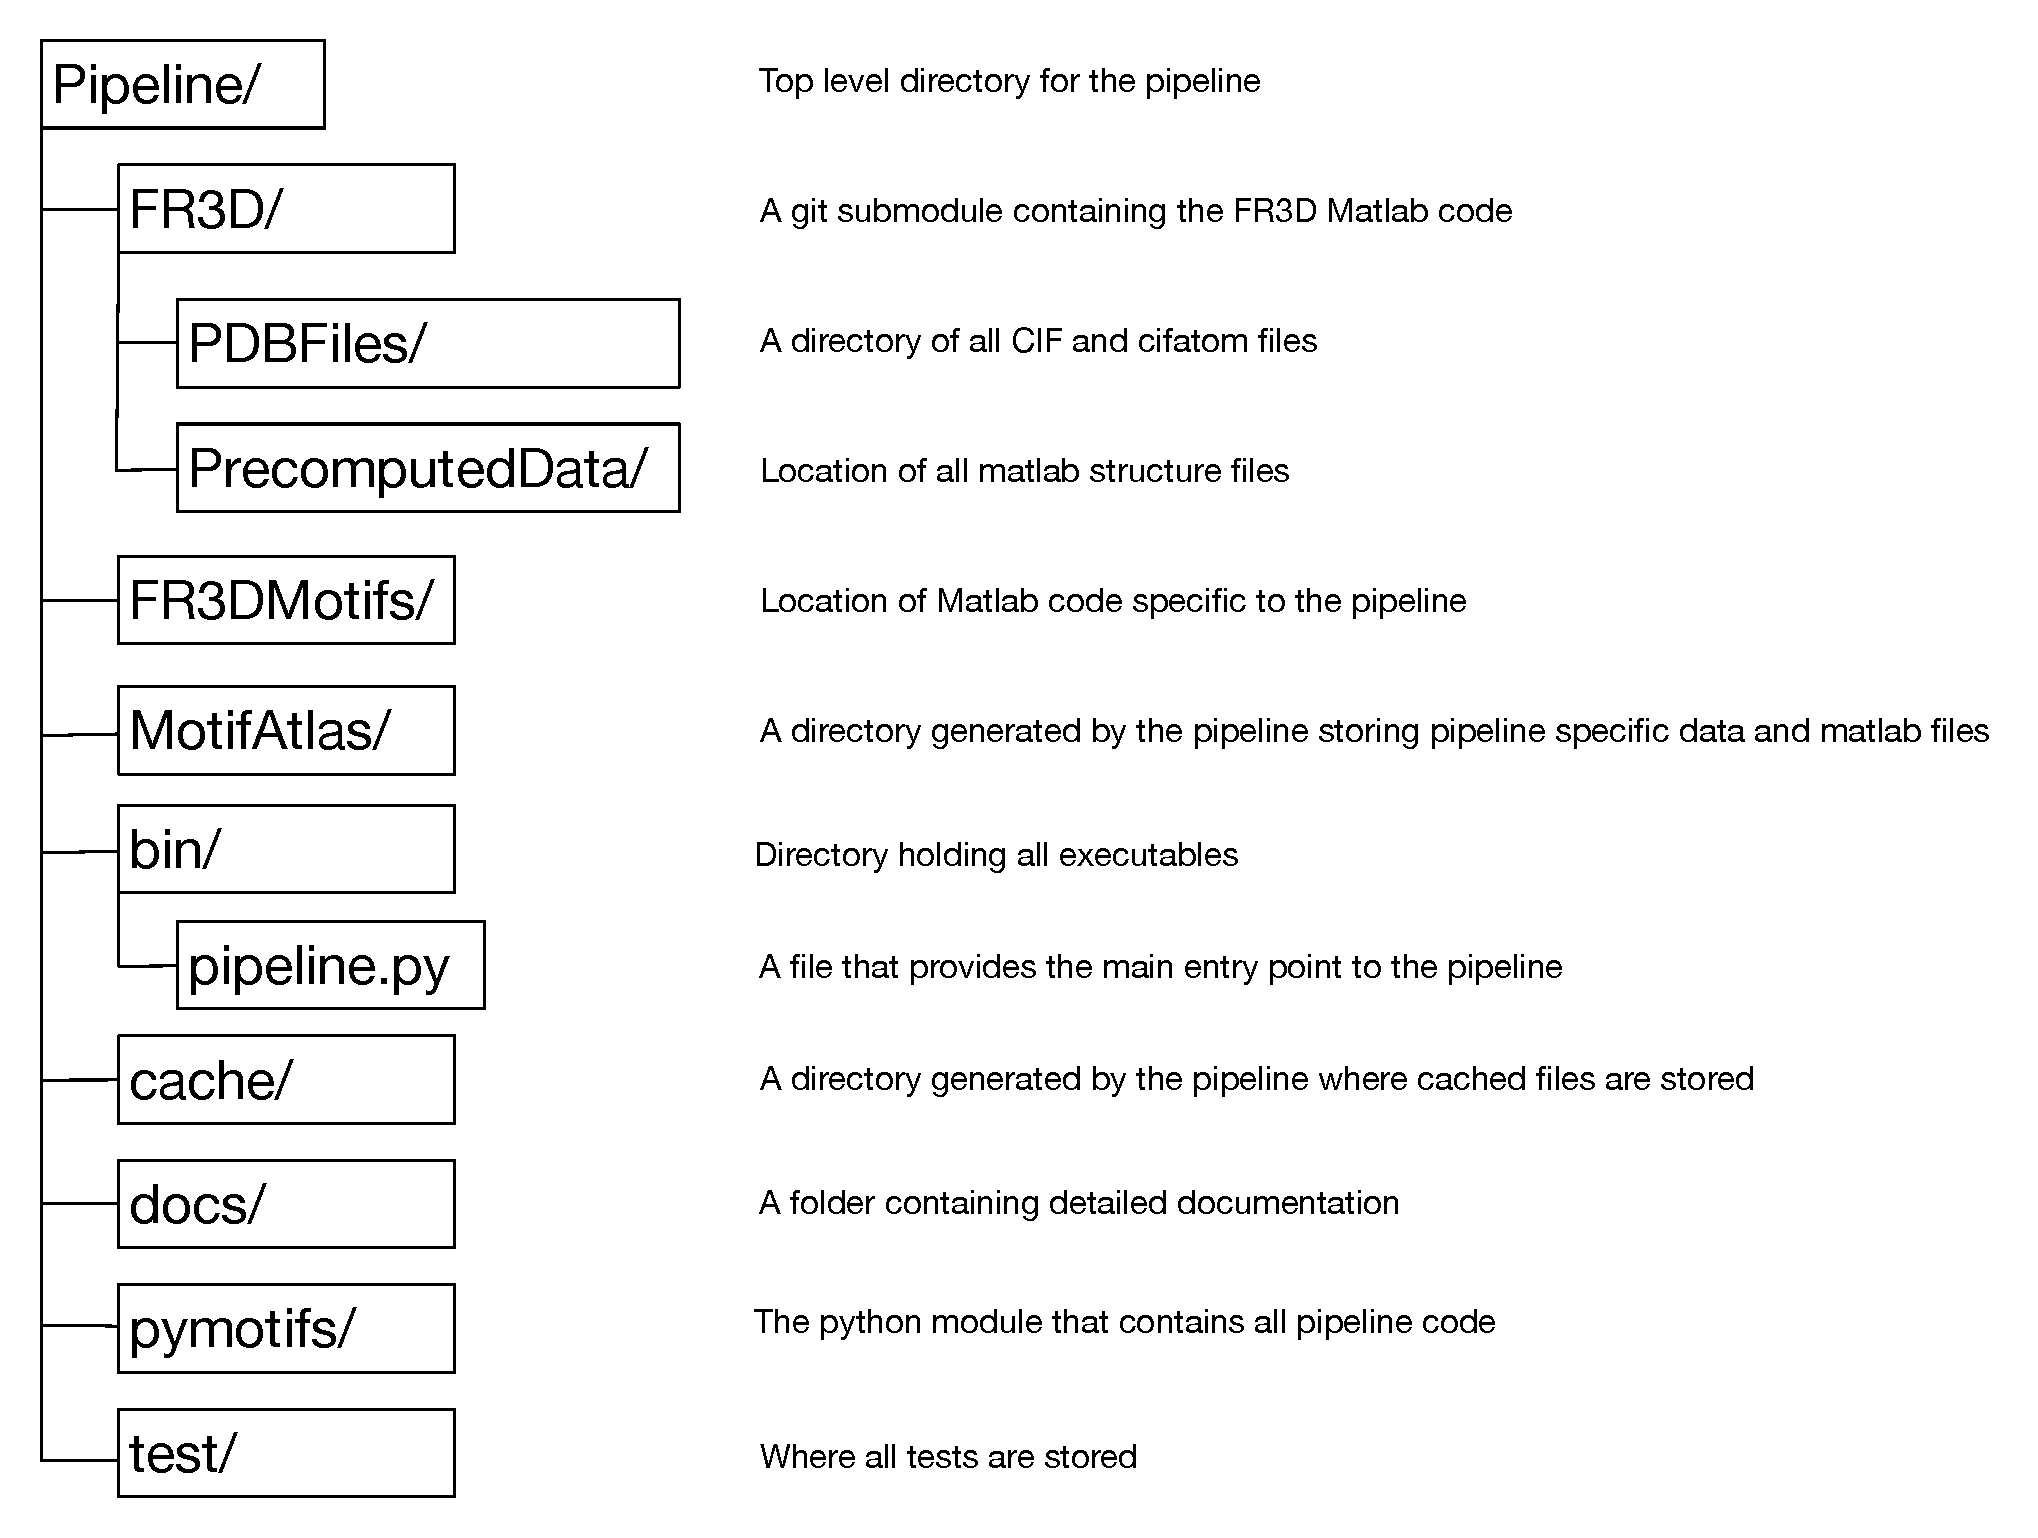
\includegraphics[width=\linewidth]{chapter-2/figs/directories}
\caption{Directory structure of the RNA BGSU pipeline. This figure shows the top
level and important directories in the pipeline. The directories are indicated
by ending with a ``/', while files do not end with a ``/'.}
\label{fig:pipeline-organization}
\end{figure}

\subsection{Configuring the pipeline}

Several important values, such as the database to use are configured in an
external file. The pipeline is configured through a JSON file that defaults to
``conf/motifatlas.json'. There are many possible configuration values, as
discussed in the detailed documentation. Table~\ref{tab:pipeline-config}
contains the key options. An example configuration file is included at
``conf/motifatlas.json.txt'' that can be modified to a simple working file. The
most important configuration value is the ``db.uri'' value which configures the
SQLAlchemy URI for the database connection. This specifies the database which to
connect to as well as the username and password. The user must be able to modify
the database, as well as add, delete and modify rows.

In addition, there are three file and directory paths which must be specified.
The first is the path to the matlab script that can execute matlab on the
command line. On linux systems this can be found using ``which matlab'' at the
command line and defaults to ``/usr/local/bin/matlab'. On OSX this will be in the
``bin/matlab'' directory below the matlab application. This means the default
location is ``/Applications/MATLAB\_R2013a.app/bin/matlab', for Matlab 2013a. The
second is where to write the loop export files. Part of the pipeline is an
export of all loops along with motif assignments. The file to write to must be
specified. Finally, the path to write interaction exports to must be specified
as well. Both the loop export an interaction export must be in a writeable
directory for the use the pipeline runs as.

Finally, the release\_mode section configures how the version numbers for motif
atlas, non- redundant and loops will be bumped. All releases follow the same
naming scheme of ``major.minor'. For example the NR release ``2.0'' has major
version ``2'' and minor ``0'. The minor can increments as much as needed and does
not influence the major version. When the major increments the minor is reset to
0. When the release\_mode is set to ``minor'' this will increment the minor part
of the version number, while ``major'' will cause the major to be bumped.
Generally, the release\_mode should be set to ``minor'. The only time ``major'
should be used is when there are large changes to the algorithm used for the
underlying algorithm.

\begin{table}[ht]
\begin{tabulary}{\linewidth}{LR}
\toprule
Variable & Purpose \\
\midrule

db.uri & SQLAlchemly uri string to specify the database to connect to \\

release\_mode.loops & A string, either ``major'' or ``minor'' to indicate
                        incrementing the major or minor version for loop releases \\

release\_mode.motifs & A string, either ``major'' or ``minor'' to indicate bumping
                        the major or minor version for motif releases \\

release\_mode.nr & A string, either ``major'' or ``minor'' to indicate bumping the
                   major or minor version for non- redundant releases \\

locations.mlab\_app & Path to matlab executable. \\

locations.interactions\_gz & Path to where the interactions export file is
                   written. \\

locations.loops\_gz & Path to where the loops export is written. \\

\bottomrule
\end{tabulary}
\caption{Main configuration options for the pipeline. All options show here must
  be provided.}
\label{tab:pipeline-config}
\end{table}

\subsection{Executing the pipeline}

The main entry point of the pipeline is the ``bin/pipeline.py'' python script. For
this discussion the script will be written as ``pipeline.py'. This script uses a
common ``subcommand'' ``options'' ``arguments'' design that will be familiar to anyone
who has used command line tools such as git. The top level command has a
``--help'' option which provides help information about the entire pipeline. In
addition, each subcommand also has a ``--help'' option to provide help information
about that command. Users should use this functionality extensively when
becoming familiar with the pipeline. In general a command to run the pipeline
looks like:

\begin{alltt}
pipeline.py [options] <subcommand> [options] [arguments]
\end{alltt}

Where $<>$ indicates a required value and $[]$ indicates an optional
value.

The pipeline provides several sets of functional facilities as shown in
Table~\ref{tab:pipeline-functionality}. This table shows each subcommand along
with the functionality it provides.

\begin{table}[ht]
\begin{tabular}{lr}
\toprule
Name & Functionality \\
\midrule
about & Get information about a stage \\
bootstrap & Populate the testing database \\
correct & A group of commands for correcting issues in the database \\
list & List the known stages and provide a breif overview \\
report & Create reports for external analysis \\
run & Run stage(s) \\
ss & Commands for importing 2D diagrams \\
transfer & Export/Import data from versions of this database \\
\bottomrule
\end{tabular}
\caption{Listing of all functionalities in the pipeline}
\label{tab:pipeline-functionality}
\end{table}

For the purposes of this section I will only discuss the import/export
functionality in the ``run'' subcommand. The main inputs to this command are the
stage to run and the structures to run it on. It takes a variety of options as
well. These options control the behavior of the pipeline. A summary of the
command is shown in Figure~\ref{fig:running-options}. Here we will discuss how
the options and arguments connect to our overall goals as well as how to achieve
some specific tasks.


\begin{figure}
\begin{alltt}
Usage: pipeline.py run [OPTIONS] NAME [IDS]...

  Run specific stages of the pipeline.

  'run' accepts as input the stage to run and a list of PDB ids to import
  and process. It determines the order of dependences and executes them in
  the correct order.

Options:
  --dry-run            Alter nothing while running
  --skip-dependencies  Skip stage(s)
  --skip-stage TEXT    Stage to skip
  --seed INTEGER       Set the random seed
  --recalculate STAGE  Recalculate data for the given stage(s)
  --all                Use all RNA containing PDBS
  --known              Use only downloaded files
  --after-date DATE    Get files posted after DATE (YYYY-MM-DD)
  --before-date DATE   Get files posted before DATE (YYYY-MM-DD)
  --exclude PDB        Excluded PDB(s)
  --ignore-time        Ignore time for rerunning
  -h, --help           Show this message and exit.
\end{alltt}
\caption{A summary of the options and arguments for the ``run'' subcommand.}
\label{fig:running-options}
\end{figure}

An important goal of our design has been to provide the user to ability to
choose the structures to process as well as the annotation data to compute. The
first was achieved by providing PDB ids as input. This input can be provided
manually when needed. It will process the files given and the user can input
them manually. As it is often the case that all available files, or all files
available by a date are wanted the pipeline accepts options which will determine
what files match that criteria. In addition, it is possible to then exclude
structures from that list using the given files.

The second goal, control over which data are computed, is done by putting the
stage to run as input to the pipeline. This provides the user precise control
over what is run. By default the pipeline will run all dependencies of the stage
as well the stage itself. This ensures that the required data are available for
the requested stage. When the user is sure that no dependencies need to be run,
I have added options to skip all dependencies ({\tt --skip-dependencies} ) or skip
specific stages ({\tt --skip-stage stage}).

Another goal is to avoid recomputing data already computed.where it is necessary
to over this default setting, the {\tt --recalculate stage} option can be used.
This option will force the pipeline to recompute all data for the given stage.
The {\tt .} stage name refers to the stage given so: {\tt pipeline.py run
--recalculate ``.'' --all units.info} will force a recompute for the units.info
stage, but not it's dependencies. To force all stages that are run to recompute,
the user can use the {\tt *} argument. For example {\tt pipeline.py run --all
--recalculate ``*'' units.info} will recompute all stages that are run for all
structures.

Examples that show how to use the described options and arguments will clarify
the usage. Below we list a series of tasks and the corresponding command
(displayed as {\tt monospaced font}).

\begin{description}
        \item [Run an update on all structures]
                {\tt pipeline.py run --all update}

        \item [Import pairwise interactions for 1FJG]
                {\tt pipeline.py run interactions.pairwise 1FJG}

        \item [Import all unit annotations for all structures]
                {\tt pipeline.py run --all units.loader}

        \item [Import all unit annotations for all structures skipping structure 2AW7]
                {\tt pipeline.py run --all --skip-pdb 2AW7 units.loader}

        \item [Create an NR group for 1FJG, 1J5E, 1S72]
                {\tt pipeline.py run nr.loader 1FJG 1J5E 1S72}

        \item [Compute all interaction annotations for all structures while skipping all dependencies]
                {\tt pipeline.py run --skip-dependencies --all interactions.loader}

        \item [Import loops in all structures]
                {\tt pipeline.py run --skip-stage loops.quality --all loops.loader}

                This command runs all loop level annotations, while skipping the loop quality stage,
                which is generally only needed before doing a motif atlas import, and simply is not
                needed importing loops, thus the reason it is skipped.

        \item [Recalculate all pairwise interactions]
                {\tt pipeline.py run --recalculate . --recalculate mat\_files interactions.pairwise}

                Note that for this command we have to recalculate all
                {\tt mat\_file}'' as well as the interaction import. This is
                because the {\tt mat\_files} stage controls the creation of the
                precomputed data that the matlab programs use. If we do not
                specify recomputing the mat files the process will simply
                reimport the already existing annotations.


        \item [Build a motif atlas using structures in the ``structures'' file]
                {\tt cat structures | xargs pipeline.py run motifs.loader}

                The structures file should contain only the ids to use, with one
                per line. The ``xargs'' command is required because the pipeline
                does not read from standard input and so xargs transforms the
                call to include the ids as part of the call. Note that there is
                a system dependent limit for the number of arguments allowed to
                a command. The limit is generally in the thousands.
\end{description}

\subsection{Testing the pipeline}

The pipeline is tested through two related methods. First, there is a script
that will run the pipeline on 70 structures to populate a test database. The
process of creating a database to work with is called ``bootstrapping''. The
structures to use are stored in ``pymotifs.constants.BOOTSTRAPPING'' and have been
chosen because they have caused crashes or errors in the past. In the future as
more problematic structures are found they should be added to the set of
structures used in testing.

The bootstrap script can be run using the command {\tt bin/pipeline.py bootstrap}.
Bootstrapping requires a special configuration file in conf/bootstrap.json. It
does not use the standard configuration file because it is important to have a
separate testing and development database. Otherwise it is possible to
accidentally overwrite or modify data that is required for tests. This can lead
to spurious test failures and waste developer time. Bootstrapping will run the
pipeline several times because one of the major parts of the pipeline is
computation of changes of groupings over time. By running it more than once on
different sets of structures we can test this important functionality.

The bootstrapping serves two purposes. The first is to populate a database the
test scripts can work with. The second is to provide a high level test of the
pipeline. By running the full pipeline on many structures we are increase the
chance of detecting blatant errors in the code. For example, bugs that prevent
the pipeline from being run will be caught here. Issues where a foreign key
constraint violation may appear here as well. This serves as a good initial
method to test the overall functionality of the pipeline and is recommended
before deploying a new stage.

The second way the pipeline is tested by ``unit testing'' components of the
pipeline. We test individual methods of classes using the py.test library. This
is a very traditional method of testing python applications. The tests are
stored in test/ and are organized into a hierarchy that parallels that of the
main program, making it simple to determine which module is being tested for
each test file. Test file names must end with ``\_test.py''. For example, the
tests for the units.info stage are in ``test/units/info\_test.py''.  There is very
extensive documentation on writing tests and readers are strongly encouraged to
read documentation on writing unit tests in python and using py.test. Examples
of such links are: 
\begin{itemize}
  \item \url{https://stackoverflow.com/questions/3371255/writing-unit-tests-in-python-how-do-i-start}
  \item \url{http://docs.pytest.org/en/latest/}
  \item \url{https://jeffknupp.com/blog/2013/12/09/improve-your-python-understanding-unit-testing/}
  \item \url{https://docs.python.org/2/library/unittest.html}.
\end{itemize}

Here we give a quick overview of testing in python, as well as information on
the parts that are unique to this pipeline.

In python, tests are often organized into classes. We use this approach
extensively in the tests. It is important to know that it is not needed, as
py.test will use simple functions as tests as well. Readers interested in that
approach should read py.test's documentation on this. We use classes because of
the organization advantages it provides. For test classes, if there is a ``setUp''
method that takes no arguments it is run prior to any tests. This method is used
to setup any data or objects that are needed for testing. As discussed below
this is used to setup stages for testing correctly. Each test method must start
with the string ``test\_'. Within them there should be an assertion about the
computed and expected value. Ideally tests are as simple as possible and contain
only 1 statement to compute the value to test, 1 statement to define the answer
and 1 statement to assert the computed value equals the expected value. This is
standard unit testing in python. The reader is encouraged to read more extensive
documentation and advice on this subject.

The test classes that test a stage in the pipeline must inherit from the
StageTest class from the test module. These classes should also have a
``loader\_class'' attribute which specifies the class of the stage to test. This
stage will be initialized in the StageTest's ``setUp'' method. The object will be
built using the configuration specified in ``conf/bootstrap.json''. As with
standard python tests this method is run prior to all test methods. Classes
which implement their own setUp method must have a call to the superclass's
setUp method. Without this the stage will not be initialized correctly.

Another useful functionality of the test suite is the ``skip\_without\_matlab''
annotation. This is to be used on any test that calls matlab. It allows the test
suite to run without crashing on machines that do not have matlab, or the python
to matlab connector, installed.

One useful extension to the testing methodology currently used is to automate
testing using a service like \href{https://travis-ci.org/}{Travis CI}. This
service reruns all tests whenever someone pushes code to the github repository.
Such testing has been implemented for the fr3d-python repository and can be seen
at \url{http://www.travis-ci.org/BGSU-RNA/fr3d-python}. Travis CI and related tools
are now standard in software development. This approach has not been used with
the pipeline for two reasons. First, setting up the database is a long and
complex procedure. The bootstrap script takes nearly half a day to run and
produces several gigabytes of data. Secondly, Travis CI and all services like it
do not have matlab installed as this is a commercial product. While the
skip\_without\_matlab annotation will ensure that other tests do not fail, it will
mean that key functionality that matlab provides will not be tested. This may
result in tests passing even though they are actually failing in an environment
with matlab. Thus we should not use the service as long as we continue to rely
on Matlab code.

It should be possible to deal with these issues by first, removing matlab from
the pipeline. Once all of FR3D's functionality is written in python the pipeline
will be testable with standard tools. Secondly, something will have to be done
to either decrease the number structures tested or make it quicker to load the
results of bootstrapping to the database. It may be possible to use a database
dump to rebuild the testing database, but that will pose problems with keeping
it up-to-date, but is worth exploring. Using a dump would mean the testing on
travis would not require the bootstrapping process, allowing for tests to be
completed quickly. Future developers should look into using tools like Travis CI
to improve the testing and reliability of the pipeline.

\chapter{GROUPING RNA 3D STRUCTURES FROM FROM PDB USING MMCIF FILES IN RNA INTO
EQUIVALENCE SETS}

\section{Introduction}

This chapter reports changes implemented to improve modules of the data pipeline
that calculates Equivalence Classes of RNA entities of RNA 3D structures for the
Nucleic Acids Database (NDB) and for RNA.BGSU.EDU. The 3D structures are
provided by the Protein DataBank (PDB).

The PDB is an archival resource that serves as  the accumulated scientific
investigation of the 3D structures of macromolecular entities of biological
significance. The earliest entries date back to the late 1960s and early 1970s
and new entries are accumulating at an ever-increasing rate. The earliest RNA
entries were structures of dinucleotides and the latest entries include entire
ribosome structures bound to a variety of tRNA and mRNA substrates and
translation factors. But structures containing smaller RNA molecules bound to
enzymes that modify them or use them as guide RNAs  to recognize other
substrates continue to accumulate. Thus there is a huge variation in the size of
the RNA entities and of the scientific purposes for which the investigation was
conducted.

\section{Previous work}

We have previously implemented a method to group RNA molecules into equivalence
sets. The method is described in Nonredundant 3D Structure Datasets for RNA
Knowledge Extraction and Benchmarking \cite{Leontis2012b}. The current work is
an extension of these methods so, we begin by briefly describing the previous
methodology which was developed when 3D structures were still distributed in PDB
files, so that like large structures like 70S ribosomes had to be split over two
or more files. At that time it was convenient to simply select the largest chain
in a file and use to represent the RNA in the file for grouping. In cases where
the file also had one or more smaller chains the smaller ones were ignored and
no groups built for them. For example, structures of a large ribosomal subunit
contain both the 23S and 5S in the same file, the 5S was simply ignored and not
extracted and clustered separately. Each chain was compared on the basis of
sequence alignment, species and geometric discrepancy to all other chains. The
previous method did not compute all possible sequence alignments or
discrepancies due to runtime issues. The alignments and discrepancies were not
stored for future studies.

\section{Motivation for current work}

We have one main motivation for updating our RNA chain grouping method. The
first is to take advantage of technical changes data and secondly are to enhance
the scientific utility of our resources by providing a more complete set of data
that includes all chains found in RNA structures.

Recently,  PDB has migrated from “PDB” formatted structure files to the new
macromolecular Chemical Information File format (mmCIF), which made it possible
to store structural information for macromolecular complexes of any size in just
one computer file. By contrast, the out-dated PDB format was limited to no more
than 99,999 numbered atom data records per file. This change has made possible
the storage of all ribosomal subunits, large subunit, small subunit, tRNA, mRNA
fragments, 5S and 5.8S (for eukaryotes) into a single file. In some files such
as 4V4Q \cite{Schuwirth2005} more than one entire ribosome is present. Because
our old method only considered the largest chain in each file we would ignore
all chains except a single LSU. This would lead to ignoring many important
groups.

There are a number of scientific use cases for which our RNA structure classes
and derived data will be  3D structures in the PDB/NDB and these are worth
enumerating and discussing.

\begin{enumerate}
  \item Determining the breadth and depth of solved structures, ie the number of
    distinct types of RNA and the number of each type.

  \item Statistical studies of recurrent elements of RNA structure, RNA-RNA and
    RNA-protein interactions

  \item Comparative studies of similar or homologous RNA structures and
    RNA-protein complexes

  \item Functional studies of RNA structural flexibility, variation and
    conformational change in response to environmental perturbations

  \item Comparative assessment of RNA structure modeling quality and reliability

  \item Compilation of modular RNA parts for synthetic biology and RNA
    nanotechnology

  \item Analysis of  of RNA sequence variation to improve RNA structure
    prediction and understanding of RNA evolution
\end{enumerate}

Thus, the change to mmCIF format required a complete rethinking of the
procedures for extracting, naming, and clustering RNA entities and has enabled
significant improvements in the results. This chapter describes those changes
and the choices made to maximize the value of the data for diverse scientific
users.

\section{Types of molecules and requirements}

In this section we will highlight specific groups that pose special challenges
for clustering to motivate the following sections were the methods developed are
explained and their success in correctly clustering these special cases is
assessed.

\subsection{Ribosomal RNA subunits}

The largest entities are ribosomal RNAs (rRNA), which comprises the large (LSU)
and small (SSU) ribosomal subunits, the 5S rRNA, and the 5.8S rRNA in
eukaryotes. LSU and SSU from a number of species representing all three major
phylogenetic domains and mitochondria are presently available.

The rRNAs should be divided into separate Equivalence Classes (EC) as follows:
First, each of the SSU rRNAs (mitochondrial 12S, bacterial 16S and eukaryal 18S
rRNAs) should be placed into their own EC by organism. Each of the 23S rRNAs
from archaeal or eubacterial ribosomes should be placed in distinct EC. The 5S
rRNAs, which are found in the LSU of all ribosomes except some mitochondrial
ones, should also be in a separate group. While bacterial 5S rRNA does interact
directly with 23S rRNA in the LSU, it does so through non-Watson-Crick pairing
and backbone interactions involving its loop E internal loop (IL) motif and a
similar structured IL of helix 38 of 23S rRNA. The loop E of 5S rRNA has been
shown to assume the same 3D conformation in the absence of 23S rRNA and so is
not dependent on 23S to form its native state. The same holds for eukaryal 5S
rRNAs, each of which are placed in their own EC.

By contrast 5.8S rRNA of eukaryal LSU, constitutes an integral part of the large
ribosomal RNAs (26S or 28S, depending on the species), as they are homologous to
the 5’-ends of bacterial 23S rRNAs. As such they form extensive Watson-Crick
interactions with the larger rRNA of the LSU in which they occur and so,
according to the criteria defined above, belong together in the same RNA entity
, for the purposes of grouping.

In addition, the ribosome has long been an molecule of study. Early structures
\cite{Mueller2000} often were resolved at very low resolution. These structures,
while informative, are not as useful for current work as more recent high
resolution structures. While we want to group all structures it is very useful
to create groups of structures with similar resolution. In the past we have
found using resolution cutoffs of 1.5{\AA}, 2.0{\AA}, 2.5{\AA}, 3.0{\AA}, 3.5{\AA}, 4.0{\AA}, 20.0{\AA}, and
‘all’ a group of all structures regardless of resolution create useful groups.
Here we continue this practice.

From these examples we can see that the members of groups should be one or more
chains which interact extensively through watson crick base pairing should be
placed as a single entity and then grouped with other such entities. We can see
that the groups should only contain molecules from the same species. In the case
of large molecules this can be determined through sequence alignments alone.
In addition, all members of a group should fall within a resolution cutoff.

\subsection{tRNA and mRNA complexes}

tRNA molecules are commonly solved in the context of their binding to a
ribosome. In these cases they are often also bound to an mRNA fragment. These
mRNA fragments can span the A and P sites of the rRNA and have two tRNA’s bound.
The mRNA fragments (6 bases) are very small and are extensively bound to the
tRNA as all bases are paired with the tRNA. Despite this we do not want to place
the tRNA’s and mRNA into a single entity for grouping. In this case we believe
the most scientifically meaningful unit is the tRNA. The small mRNA fragment is
not interesting alone. It is small and contains no internal structure. Thus
while we do want to place two chains which extensively pair into a single unit
we do not want small unstructured chains connecting two larger structured
chains. For the purposes of grouping all chains we will allow the small
unstructured chain to ‘accompany’ the larger chains. But it should not be used
to connect the two structured chains.

The tRNA case also provides another case to consider. It is well known that some
initiator tRNA's from different species have the same sequence. This implies we
cannot use sequence alignments alone to separate molecules from different
organisms. However, there authors provide a source organism annotation.
Investigations into this annotation have showed that while many are precise some
annotations include the terms ‘synthetic compound’ or are not provided. These
chains often have identical sequence to another annotate chain. In other cases
the synthetic chain aligns very well to a correctly annotated chain. Thus we can
treat synthetic or no annotation as being similar to any other annotated
species.

These issues, the fact that some molecules from different organisms will have
identical sequences, and the potential issues with author annotations shows us
that while we should use alignments and organism assignments to connect members
of a group we must provide another criteria. We must enforce that each group
contain a single species, ignoring the assignments to synthetic. This will
maintain our requirement that groups contain only members from the same species.

\subsection{Small model compounds}

A great deal of detailed structural information has been provided by studies of
small model compounds. These compounds are often two strands which bind to form
a small helix with loops. For example studies of the isolated sarcin-ricin motif
(CITE: 4NLF) have provided detailed information on its structure. In these
structures the unit we should cluster is the duplex. Like the LSU and 5.8S each
strand interact extensively through Watson-Crick base pairs. However, these
strands have no internal structure. There are also model compounds, such as the
nano square that are composed of 8 chains \cite{Dibrov2011a}.

From these examples we can see that we should be able to join any number of
unstructured chains together to form a single unit for grouping. This is
different from the case of multiple tRNA's on a small mRNA fragment where the
two tRNA's would not form a single unit. Here we want the chains, even if they
are not directly interacting, to form a single unit.

Many of these small model compounds differ from one another from due to single
nucleotide changes. These changes are intentional and so we require that small
molecules have identical sequences in our grouping.

\subsection{Small Protein and RNA complexes}

Several proteins have been solved with small bound RNA's. These RNAs are often
poly-A or other such simple sequences. These chains may agree in sequence and
species assignments but they differ in assigned geometry due to binding by the
protein. These chains should be split even if they are similar on the basis of
sequence and species. Thus our groupings should be sensitive to the overall
geometry of the members.

\section{Criteria for equivalence classes and their members}

These examples show first of all, that many CIF miles contain more than one
chain. Second the example of Eukaryotic LSU rRNA show that the members of some
EC may be one or more chains in contrast to our previous EC. A prerequisite of
grouping is to define the RNA-containing entities to be extracted from structure
files as precisely as possible and in a manner that is biologically relevant for
the purposes of most users of the resource. Guided by giving priority to
biological relevance, we settled on the following definition of the relevant
RNA-containing entities: The entities to be identified and extracted from
PDB/NDB structure files are “groups of one or more RNA chains that form
identifiable integrated structural and functional units.” Internally we refer to
these entities as “RNA integrated functional elements” or “RNA IFEs.” We will
use the term “IFE” as a short-hand for this definition.  Most RNA IFEs consist
of a single chain, but some do not. The simplest examples comprise two chain
Watson-Crick paired chains forming a duplex structure: strictly, this comprises
two molecules, but effectively it is a single entity or RNA IFE.

From these examples we can see there are 3 requirements for each EC.
\begin{enumerate}
  \item Two IFE’s included in the same Equivalence Class should come from the
    same biological source. The intention of this criterion is to separate
    homologous RNA molecules, for example SSU rRNAs from different organisms,
    into distinct Equivalence Classes.

  \item Two IFE’s included in the same IFE should have very similar, though not
    necessarily identical sequences. This criterion may seem redundant with the
    first criterion. The intention is to include sequence variants (for example
    16S rRNAs coded by different genes of the same micro-organism that differ in
    a small number of positions) but to separate molecules with similar
    sequences from evolutionarily related organisms that belong to distinct
    species. We note that not all RNA chains in PDB are labeled with a
    biological source, which complicates clustering.

  \item Two IFE’s included in the same Equivalence Class should have the similar
    conformations and geometries. The intention of this criterion is to separate
    instances in which there is a significant conformational change, even when
    the RNA sequence(s)and biological source  are the same. For example, poly-A
    bound to poly-A binding protein (PAB) (PDB 1CVJ) has a different
    conformation from poly A forming a parallel strand duplex (PDB 4JRD). These
    IFE’s are structurally dissimilar and should not be in the same equivalence
    set, even though the sequence may be identical.

  \item Two IFE’s included in the same EC should have similar resolution.
\end{enumerate}

However, we decided to group structures together even though their sizes differ
when:

\begin{enumerate}
  \item The same molecule was used in the experiment as reported in the CIF data
    field ``poly\_seq\_scheme''. In some cases only part of the molecule was
    resolved. Because the experiment was using the same molecule we believe it
    should be grouped with the other structures of the same, but larger
    molecule.

  \item The observed part superposes well with the corresponding parts of more
    completely resolved structures.

  \item The observed structure is a small part of the overall molecule. For
    example, there are structures of a single domain of the ribosome
    \cite{Nissen2000}. These structures are best grouped with the other
    ribosomal structures as that is the context they are just a small portion of
    the larger complex.
\end{enumerate}

In addition, there are several other cases where we assign IFE’s to the same
equivalence set:

\begin{enumerate}
  \item We group IFE’s together EVEN WHEN their geometries differ significantly
    when the structures are too low resolution as the data are not adequate to
    quantify the structural differences.

  \item Structures belong together even when RNA is bound to different proteins
    or ligands but they have when they have very similar geometries. At present,
    it is not our intention to classify PDB structures at the level of
    RNA-protein complexes. For this study we focus on the RNA components of the
    structure.
\end{enumerate}

There are several important implications of these requirements. First it is
possible that the homologous RNA molecules (for example iso-accepting tRNAs)
from different species have nearly identical sequences and structures.
Nonetheless they will be placed in different groups In addition, it is possible
that two groups will have similar sequence and species but differ only in
geometry.

\section{Methodology for building Equivalence Sets}

In this section we discuss the process of building equivalence sets. The overall
process is to
\begin{enumerate}
  \item Identify and extract RNA chains

  \item Build RNA IFE's from individual chains.

  \item Link pairs of IFE's by sequence similarity, source species, and
    geometric similarity.

  \item Extend equivalence sets using transitivity of similarity links

  \item Assign names

  \item Display data on our Website

  \item Share data with NDB
\end{enumerate}
Below we discuss each step in detail and how it achieves our goals.

\subsection{Building RNA IFE's from individual chains}

We have implemented an algorithm for joining chains into IFE's. As discussed in
our examples the joining logic depends on whether or not a chain is
``structured''. Structured chains only get joined with other structured chains
they directly interact with, and they must make a significant number of
interactions with them. Unstructured chains are always joined any chain they
interact with, but they will not indirectly join two structured chains together.

Our algorithm operates as follows. We first mark all chains in a structure as
``structured'' or ``unstructured''. A ``structured' chain is defined by having at
least 5 internal (within the same chain) cis Watson Crick/Watson Crick (cWW)
basepairs. We then join chains based upon a few rules. A representation of these
rules is shown in Figure~\ref{fig:build-ife}.

\begin{figure}
  \includegraphics[width=\linewidth]{chapter-3/figs/build-ifes}
  \caption{The rules for building connecting chains into IFE's. Each chain is
    represented by a circle. Unstructured chains are in blue with the letter
    ``U'', while structured chains are orange in ``S''. The left side indicates the
    input and the right shows the possible results of each case. On the left the
    dotted lines indicate one or more cWW interactions between the chains. On
    the right each grey circle indicate an IFE built of the two chains. For case
    1 and 2 we always join the two chains into one IFE, while in case 3 it
    depends upon the number of interactions. Case 4 shows that for two
    structured chains selected by an unstructured chain the two structured
    chains are placed in separate IFE’s while the unstructured chain is placed
  in both IFE's.}
  \label{fig:build-ife}
\end{figure}

In this figure we can see the four basic cases. First when determining if we
unstructured chains should be connected, we always connect them if they have any
cWW interactions between them. This allows for joining of separate stands of
duplexes. In the second case we always connect unstructured chains to structured
chains. This serves to connect unstructured fragments such as mRNA’s to the
structure tRNA’s they are interacting with. For connecting two structured chains
we require that the maximal ratio of external cWW to internal basepairs is at
least 0.6. This is an experimental determined cutoff. It may be adjusted in the
future. To examine if this cutoff is reasonable we produced the figures shown in
Figure~\ref{fig:ext-vs-int}.

\begin{figure}
  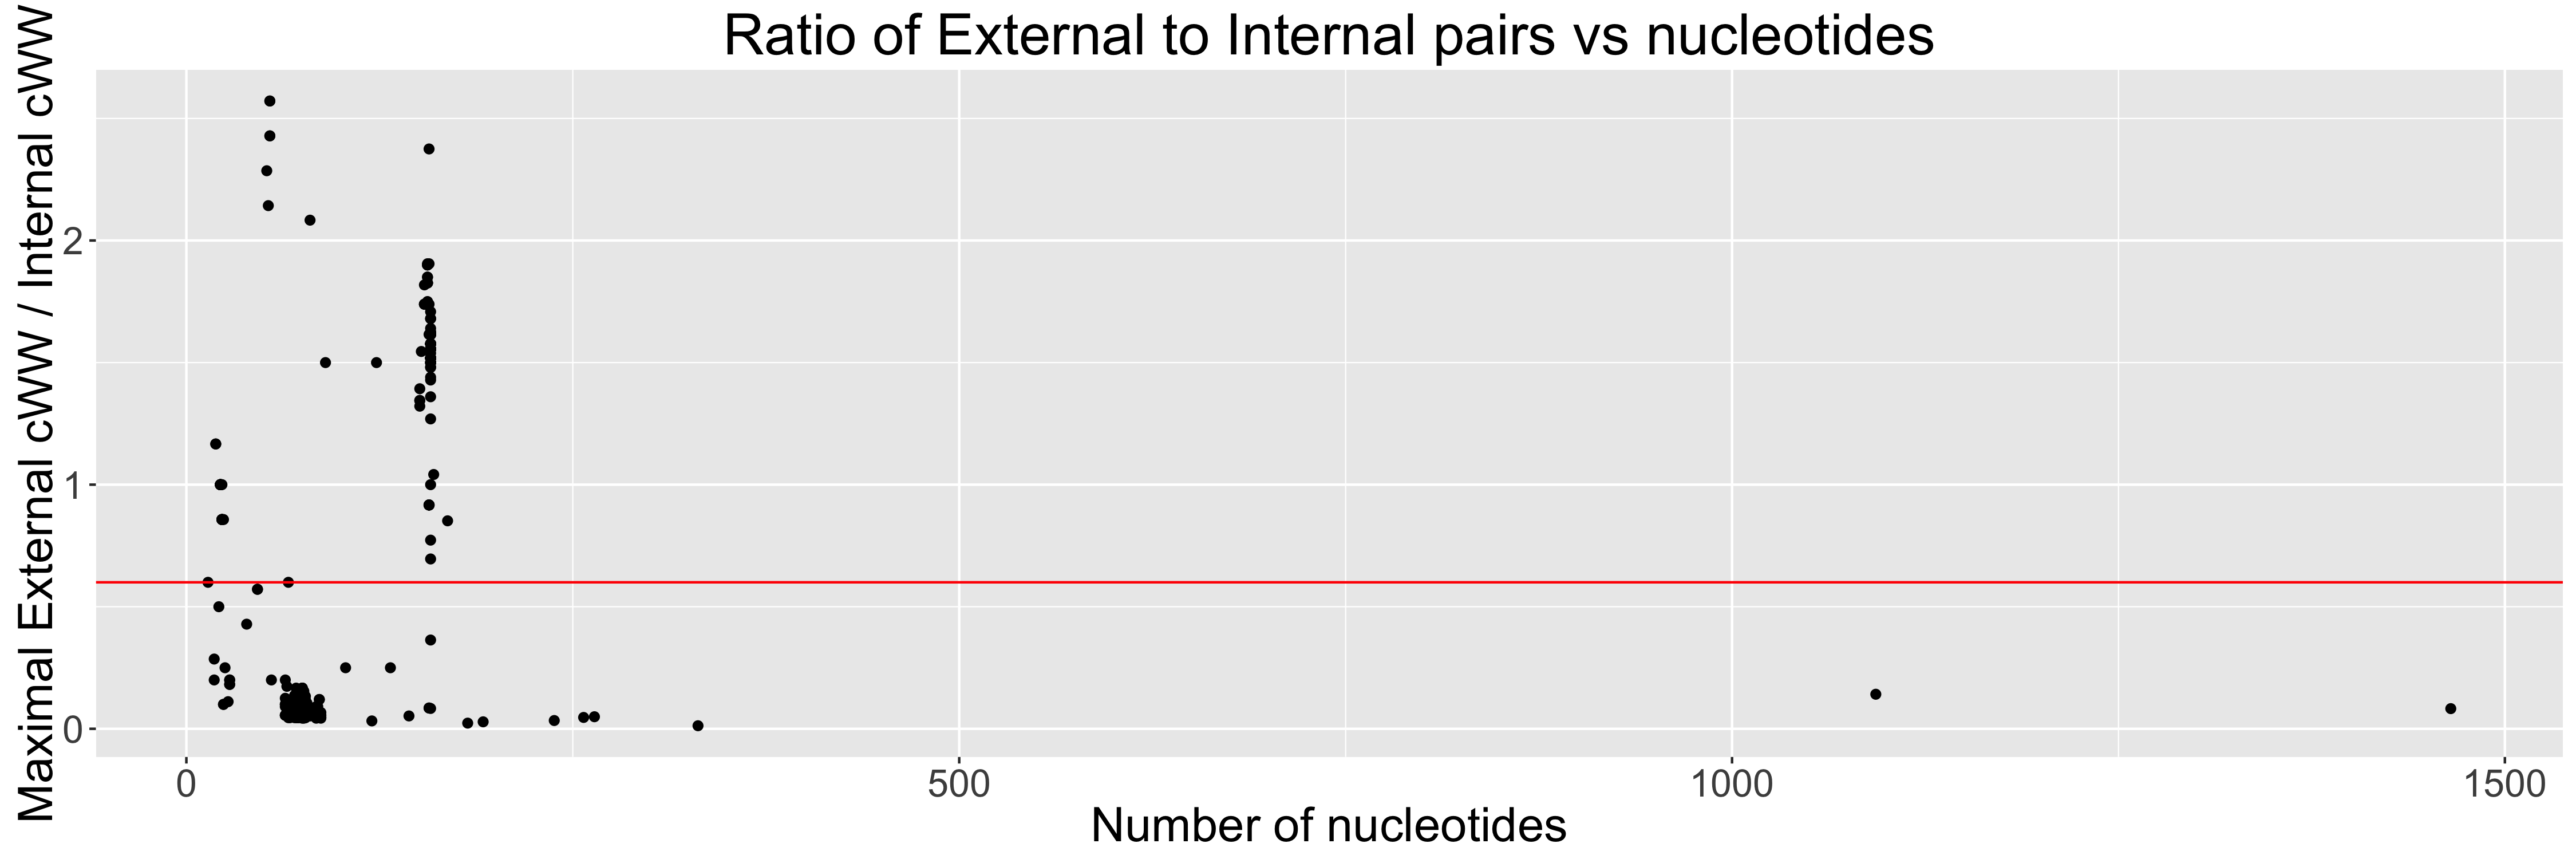
\includegraphics[width=\linewidth]{chapter-3/figs/internal-external}
  \caption{Summary of the ratio of external to internal base pairs. The leftmost
    panel shows a histogram of the maximal ratio of external to internal pairs
  for all pairs of chains which have an interaction between them. }
  \label{fig:ext-vs-int}
\end{figure}

\subsection{Connecting pairs of IFE's to from equivalence sets}

To build equivalence sets we compare all pairs of IFE’s based upon their species
assignments, their alignment, their discrepancy. Pairs of chains which have a
valid alignment, are from similar species and have a discrepancy of less than
0.4{\AA}, if computed, are joined. We then build the EQ sets by placing all chains
which are transitively connected into one set.

The steps are:
\begin{enumerate}
  \item Determine the species assignment for all chains.
  \item Compute the alignment of all pairs of alignable chains.
  \item Compute the discrepancy between all chains which have a good alignment
\end{enumerate}

The first step requires looking up the assigned phylogeny for chain. Many chains
are assigned to a particular species making the lookup trivial, however some are
assigned to a subspecies. For these cases we use the parent species of the
chain. However, not all chains are assigned to an organism, many are marked as
‘synthetic construct’ or not assigned any organism. In both of these cases we
treat the organism as synthetic. In addition, a few chains (3) are assigned to a
genus rather than a species or sub-species, in these cases we treat the chain as
being synthetic as well.

In order to compute the alignments between all pairs of chains correctly and in
a reasonable time frame we align experimental sequences. Experimental sequences
are the sequences used in the experiment and may differ from what is observed in
the experiment. Often the solved structure will have ‘gaps’ indicating where
bases were not resolved. For example EXAMPLE. In order to build alignments
correctly we use the experimental sequence. If we did not we would have to
ensure that the resulting alignments respected gaps in the both chains. The
alignments would  have to have breaks where the observed chains have breaks.
This is a difficult problem and it is simpler to use the experimental sequences
where this is not a concern.

In addition, by using experimental sequences we reduce the number of required
alignments. It is very common to use the same molecule in many experiments. For
example, there are many structures of the same E. coli ribosome with different
tRNA’s or antibiotics. All of these structures can be represented by a few
experimental sequences. There is no need to realign sequences simply because
they came from different experiments, the alignments will be the same.

We also require that all the pairs of experimental sequences to align  have
similar size. The rules for size depend upon the size of the chain. The specific
rules are shown in TABLE SIZE RULES. The reason for the size constraint is to
reduce the number of required alignments while ensuring that we perform all
required alignments. For our purposes an alignment between a large and small
subunit will never provide any information so we avoid computing them.

Finally, we require that the experimental sequences have either been assigned to
the same species or one of them has been assigned to synthetic. We refer to this
as the chains having a similar species. This ensures that we are only comparing
sequences which could be from the same source. We have observed that some
experimental sequences are assigned ‘synthetic’ in one experiment are assigned a
species such as E. coli in another experiment. Thus we allow the comparison of
synthetic chains to any other chain, so long as it has similar size. The last
step is to compute the discrepancy. Discrepancy is a measure of geometric
similarity like RMSD but it is sensitive to the base orientation and position.
It has been used extensively in our lab for searching RNA 3D Structures
\cite{Sarver2008a}, building NR sets in the past \cite{Leontis2012b}, as well as
building motif groups \cite{Petrov2013}. We only use the first structured chain
in each IFE. While this is a simplification of the situation it has proven to
work well and makes the problem simpler. For discrepancy we are only interested
in chains that:

\begin{enumerate}
  \item Have a good alignment between them. As this discrepancy will be used to
    build EC, there is no need to compute it for chains that do not align well.
    These chains cannot be in the same EQ set so discrepancy is not needed. This
    reduces the number of comparisons needed making the computations much
    quicker.

  \item Have resolution less than 4.0{\AA} or are solved using NMR. We do not
    compute discrepancies for chains with poor resolution (greater than 4.0{\AA})
    because doing so provides artificially inflated value. Many structures of
    low resolution are helices which have not been modeled with planar paired
    bases. This modeling is inaccurate and produces high discrepancy when
    compared to carefully modeled helices. Because of this we split structures
    which should be joined. We however, do allow for comparisons using NMR
    because most NMR structures are very small and the errors introduced are
    small.

  \item Have at least 3 aligned bases. This is because discrepancy is only
    defined for at least 3 bases.

\end{enumerate}

With these rules we are able to efficiently compute all required discrepancies.
By doing this as part of our pipeline we are able to store these values. This
allows for comparison of grouping methodologies and constraints.

We then connect all pairs of IFE’s which satisfy the alignment, species and
discrepancy requirements. These connections are treated as a graph and used to
build equivalence classes through transitivity.

\subsection{Building equivalence classes from pairs of IFE’s}

We build EC through transitivity. This means that all connected IFE’s, even if
the connections are indirect, are placed into a single group. An example of such
a clustering is shown in Figure~\ref{fig:transitivity}.

\begin{figure}{ht}
  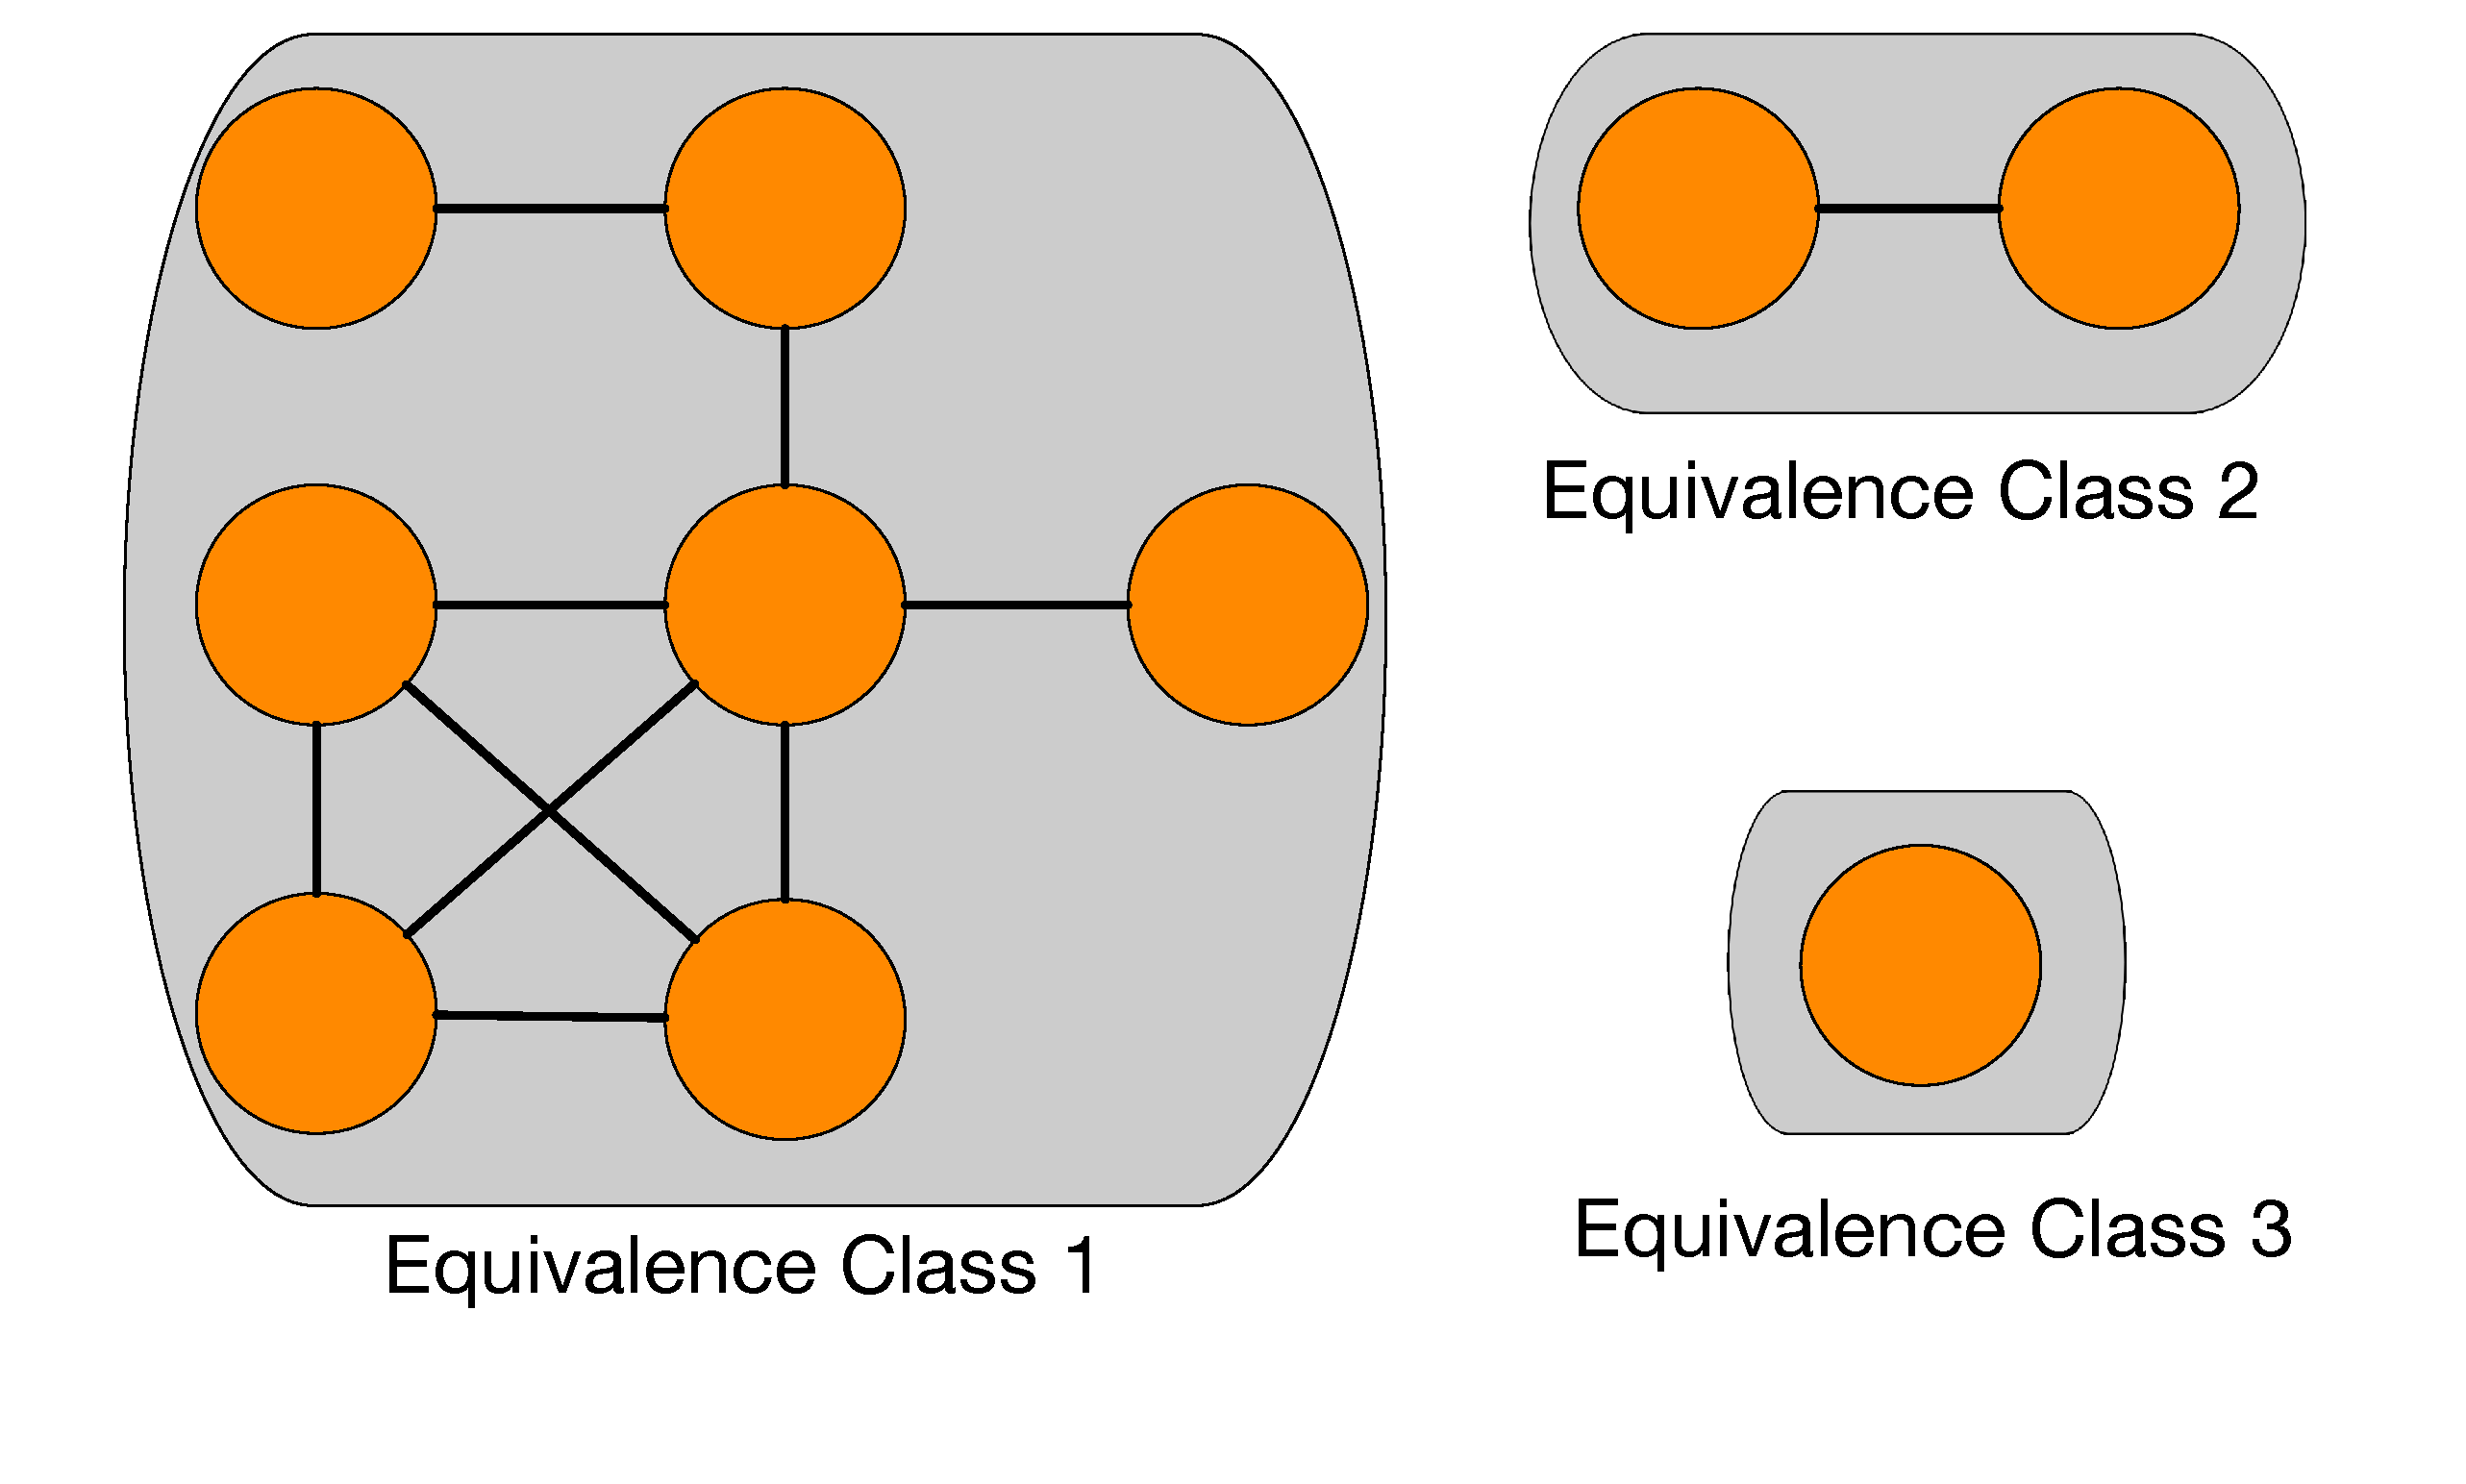
\includegraphics[width=\linewidth]{chapter-3/figs/ife-transtivity}
  \caption{Schema of Equivalence Classes built by transitivity. In this figure
    each IFE instance is represented by a circle.Lines connecting circles
    indicate pairs of IFE's having similar sequences, the same species and
    geometric discrepancy below the threshold value of 0.4. Each Equivalence
  Class is represented by the grey background around a set of circles. To in
included in a class an instance need only be connected to one other member of
the class.}
  \label{fig:transitivity}
\end{figure}

Using transitivity minimizes the number of singleton outlier groups. Most IFE’s
will compare well to at least one other, placing them in the same group. The use
case of studying structural variation in molecules. Without a transitive
grouping, structures which differ only in structure would be split from all
other instances. The groups are created using all possible structures, the ‘all’
resolution cutoff. From there the groups are filtered to only contain structures
which satisfy each resolution threshold. With the groups created, the only
remaining step is to name them

\subsection{Naming equivalence sets}

In previous work Dr. Anton Petrov created a naming scheme based upon the
parentage of the equivalence class \cite{Petrov2013}. I preserve the overall
scheme but have modified it in a significant way to make an easier to understand
system, as described next.

The naming scheme is as follows:
``NR\_{resolution\_cutoff}\_{unique\_handle}.{version}''. This scheme has 3
components, the resolution cutoff used, a unique randomly selected handle and
the version number for this group. The resolution cutoff provides information on
what the resolution is used to build the EQ set. The unique handle is a unique
randomly generated number that serves to make all ids unique.

We have changed the naming scheme so that the unique handle is identical across
all resolution cutoffs of the same set of structures. For example, an EQ set
built of tRNA’s at the ``all'' resolution cutoff may have the name:
``NR\_all\_00001.1''. At the 4.0{\AA} resolution cutoff this now would have the
name ``NR\_4.0\_00001.1''. This differs from the previous method where as
different randomly generated handle was assigned to each resolution cutoffs of
the same equivalence set. By making this change the random handle remains
identical across resolution cutoffs making it much easier to which EQ sets have
the same molecule.

\section{Results of Equivalence Set building}

For the purposes of this chapter we created an EQ grouping using all structures
available as of July 25, 2016. This grouping was then analyzed to see how the
resulting groups matched our objectives. I begin with a general description of
the clustering and then discuss each previously mentioned case in detail,
finally I examine the groupings of outliers.

\subsection{General properties}

I built a grouping using all PDB available from July 28, 2016. The grouping used
3213 PDB’s which contained 7015 IFE’s. These were grouped into 2168 EC’s. These
groups varied in size from 1 (singleton groups) to 377 instances. A summary of
the member count distribution is shown in in Table~\ref{tab:eq-size-dist}.

\begin{table}
  \begin{tabular}{lr}
    \toprule
    Number of instances & Number of Equivalence Classes (Percent of all classes) \\
    \midrule
    1               & 1352 (62.4\%) \\
    2-5             & 615 (28.3\%)  \\
    5-10            & 118 (5.4\%)   \\
    10-20           & 53 (2.4\%)    \\
    20-50           & 16 (0.7\%)    \\
    \textgreater 50 & 14 (0.6\%)    \\
    Total           & 2168 (100\%)  \\
    \bottomrule
  \end{tabular}
  \caption{Counts of the number of classes for a range of sizes. This table
    shows the number of classes for a range of sizes for the new grouping method
  for all 3213 structures available as of July 28, 2016}
  \label{tab:eq-size-dist}
\end{table}

The table shows a surprisingly high percentage, 62\%, of singleton groups. I
tested to see if this is consistent with the previous method by building a
grouping using the set of structures December 05, 2014 as shown in
Table~\ref{tab:compare-size-dist}. This date was chosen because it corresponds
to both the last grouping using our previous method as well as as the transition
to mmCIF data. These two datasets contain the same experimental results, however
there are fewer mmCIF files because many  of the PDB files have been merged into
a single mmCIF file. This gives us an ideal set to compare the two methods. From
the table we can see that the old and new method have similar performance, with
the new one having fewer singleton groups. Thus 62\% of our groups are singleton
groups for the July 28, 2016 data is not surprising when compared to the
previous groupings.

\begin{table}
  \begin{tabulary}{\linewidth}{LRR}
    \toprule
    Number of instances & 
    Number of Equivalence Classes in 2.0 & 
    Number of Equivalence Classes in 1.89 \\
    \midrule
    1               & 1081 (61.0\%)  & 1112 (78\%) \\
    2-5             & 527 (30.0\%)   & 234 (16\%)\\
    5-10            & 88 (5.0\%)     & 31 (2\%)  \\
    10-20           & 38 (2.0\%)     & 19 (1\%)  \\
    20-50           & 20 (1.0\%)     & 8 (0.5\%) \\
    \textgreater 50 & 11 (0.6\%)     & 5 (0.3\%) \\
    Total           & 1765 (100\%)   & 1409 (100\%) \\
    \bottomrule
  \end{tabulary}
  \caption{Comparison of new method to previous method. This table compares the
  performance of the previous and new method on the same data set of structures.
The data are taken from
\url{http://rna.bgsu.edu/rna3dhub/nrlist/download/2.0/all/csv}, which contains 2680
structures, and \url{http://rna.bgsu.edu/rna3dhub/nrlist/download/1.89/all/csv}
(contains 3145 structures) and represents all the structures available as of
December 5, 2014. The transition from 1.89 to 2.0 corresponds to the move from
PDB to mmCIF formats which decreased the total number of files, because many
previously separate files were merged}
  \label{tab:compare-size-dist}
\end{table}

I next moved to examine results of groups of particular interest. I begin with
the ribosomes, then tRNA’s, and then protein/RNA complexes.

\subsection{Ribosomal subunits}

As an example to evaluate the groupings of ribosomes, I examined the equivalence
classes containing the Thermus thermophilus small ribosomal subunit (SSU). We
constructed heatmaps of both the sequence similarity and the discrepancy between
all chains as shown in Figure~\ref{fig:tt-ssu-align} and
Figure~\ref{fig:tt-ssu-disc}. The alignment heatmap indicates the high sequence
similarity among all IFE’s. The geometric discrepancy heatmap shows that there
may be two main structurally groups in the equivalence class. Currently we are
exploring these groups to see if they correlate to biological states.

\begin{figure}[h]
  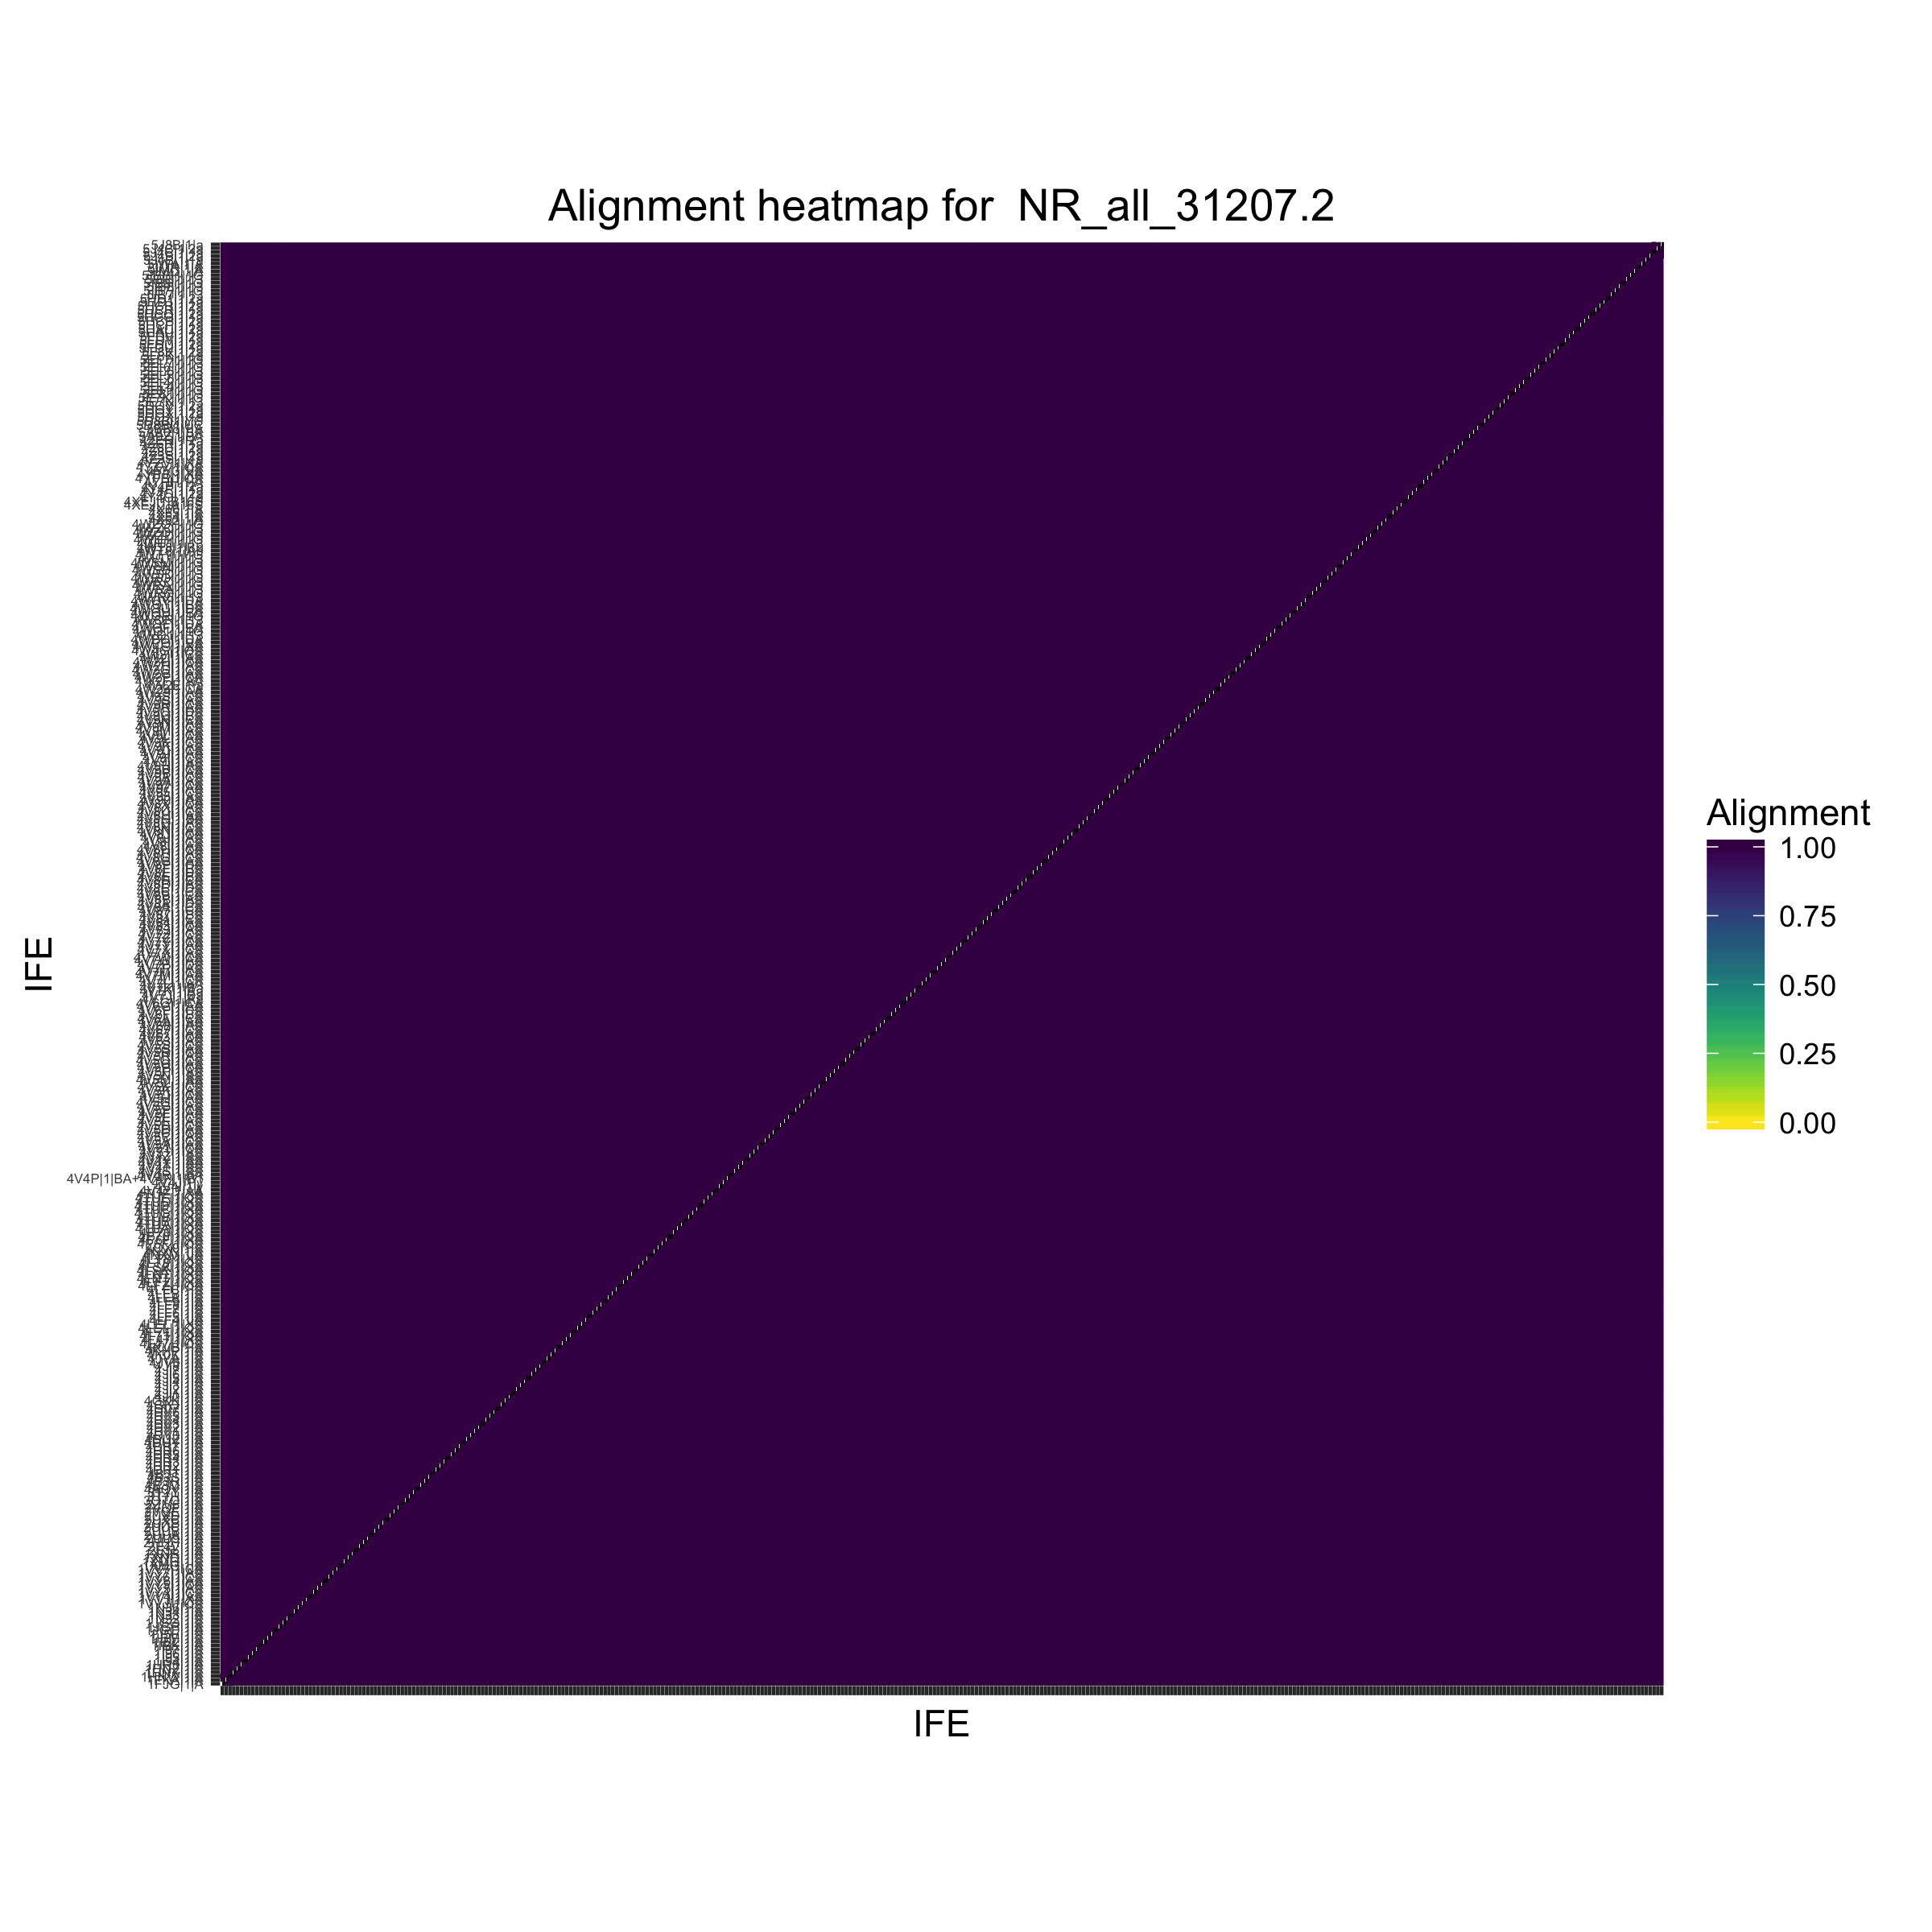
\includegraphics[width=\textwidth]{chapter-3/figs/tt-ssu-align}
  \caption{A figure summarizing the sequences similarity for all IFE’s in the
    Thermus thermophilus small subunit. Color scale indicates discrepancy
  values, lighter colors being worse.}
  \label{fig:tt-ssu-align}
\end{figure}

\begin{figure}[h]
  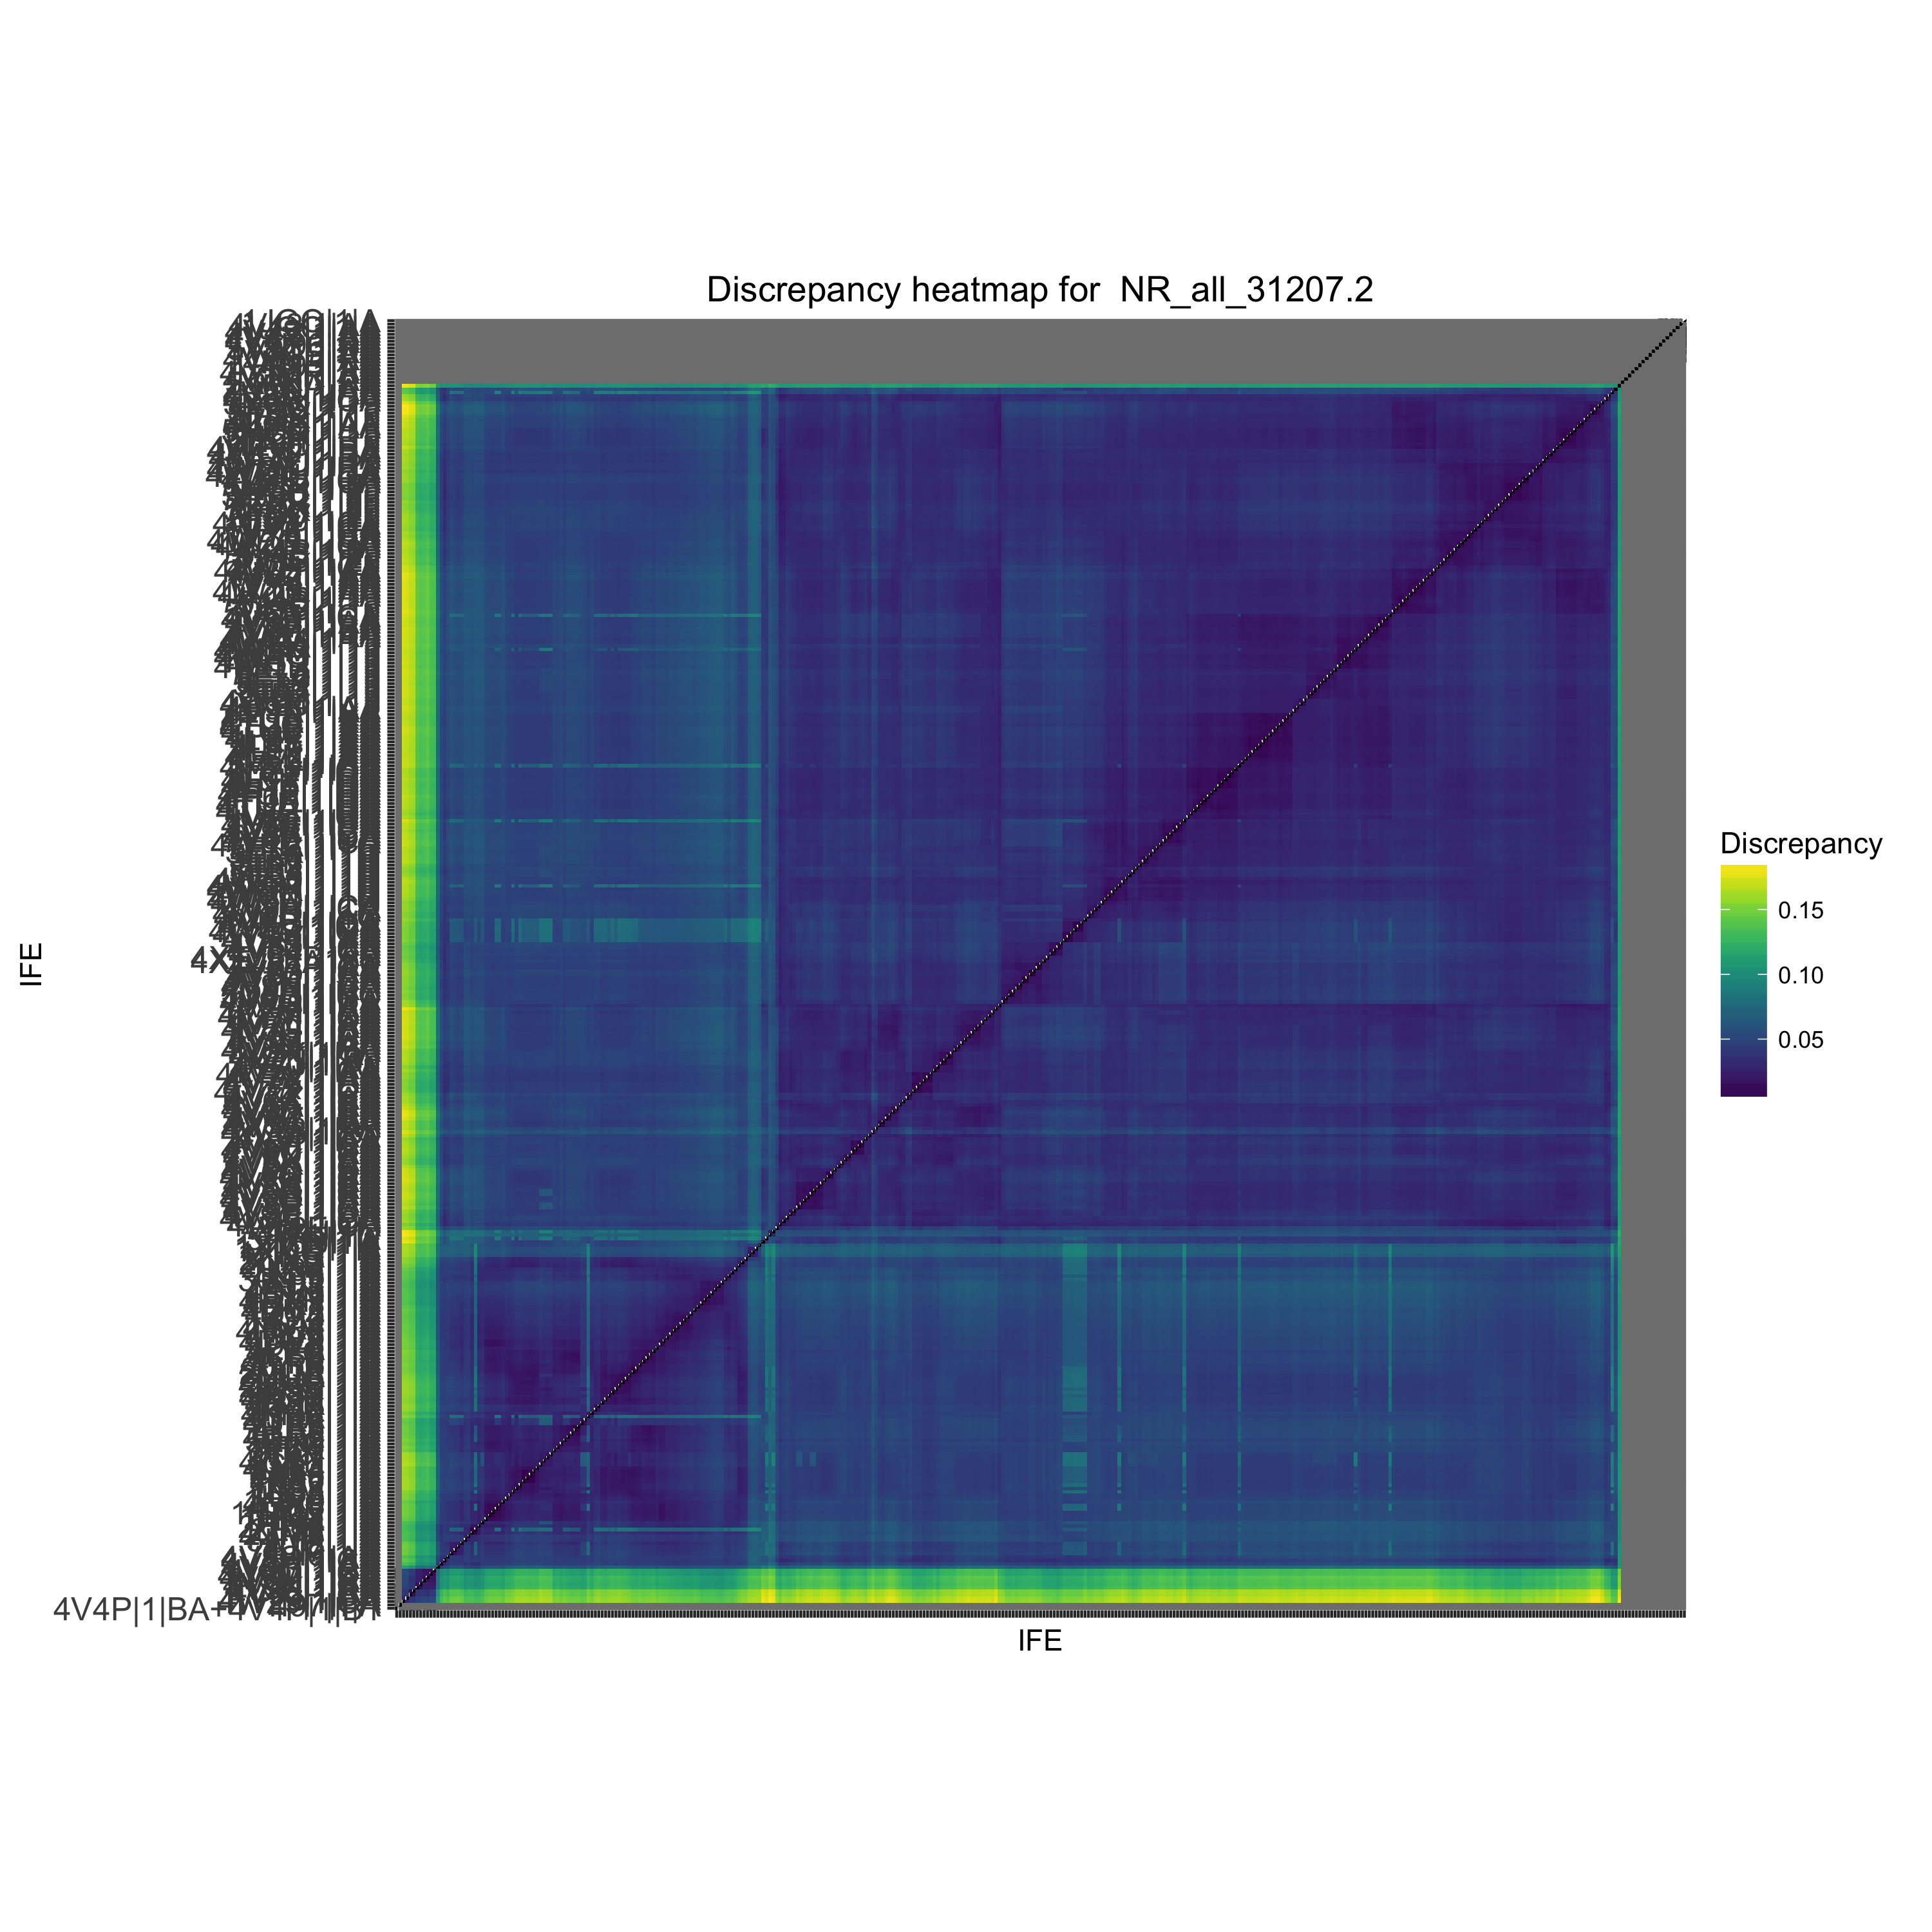
\includegraphics[width=\textwidth]{chapter-3/figs/tt-ssu-disc}
  \caption{Summary of the discrepancy for all pairs of IFE’s in the Thermus
    thermophilus small subunit. Grey squares indicate no data computed, because
    that structure has too low a resolution. Color scale indicates discrepancy
  values, lighter colors being worse.}
  \label{fig:tt-ssu-disc}
\end{figure}

\subsection{tRNA and mRNA complexes}

We examined two classes that contained tRNA alone and tRNA/mRNA complexes. The
tRNA only group is shown in Figure~\ref{fig:trna-alone}. In it we can see that all
chains are geometrically similar and have identical sequences. However, within
the group we can see that there are several subgroups, notably, 4WSM chains 2L
and 2K are geometrically distinct from all other members and similar to each
other. However, the differences are below our cutoff of 0.4 {\AA}/nt leading to them
being placed in the same group.

\begin{figure}[h]
  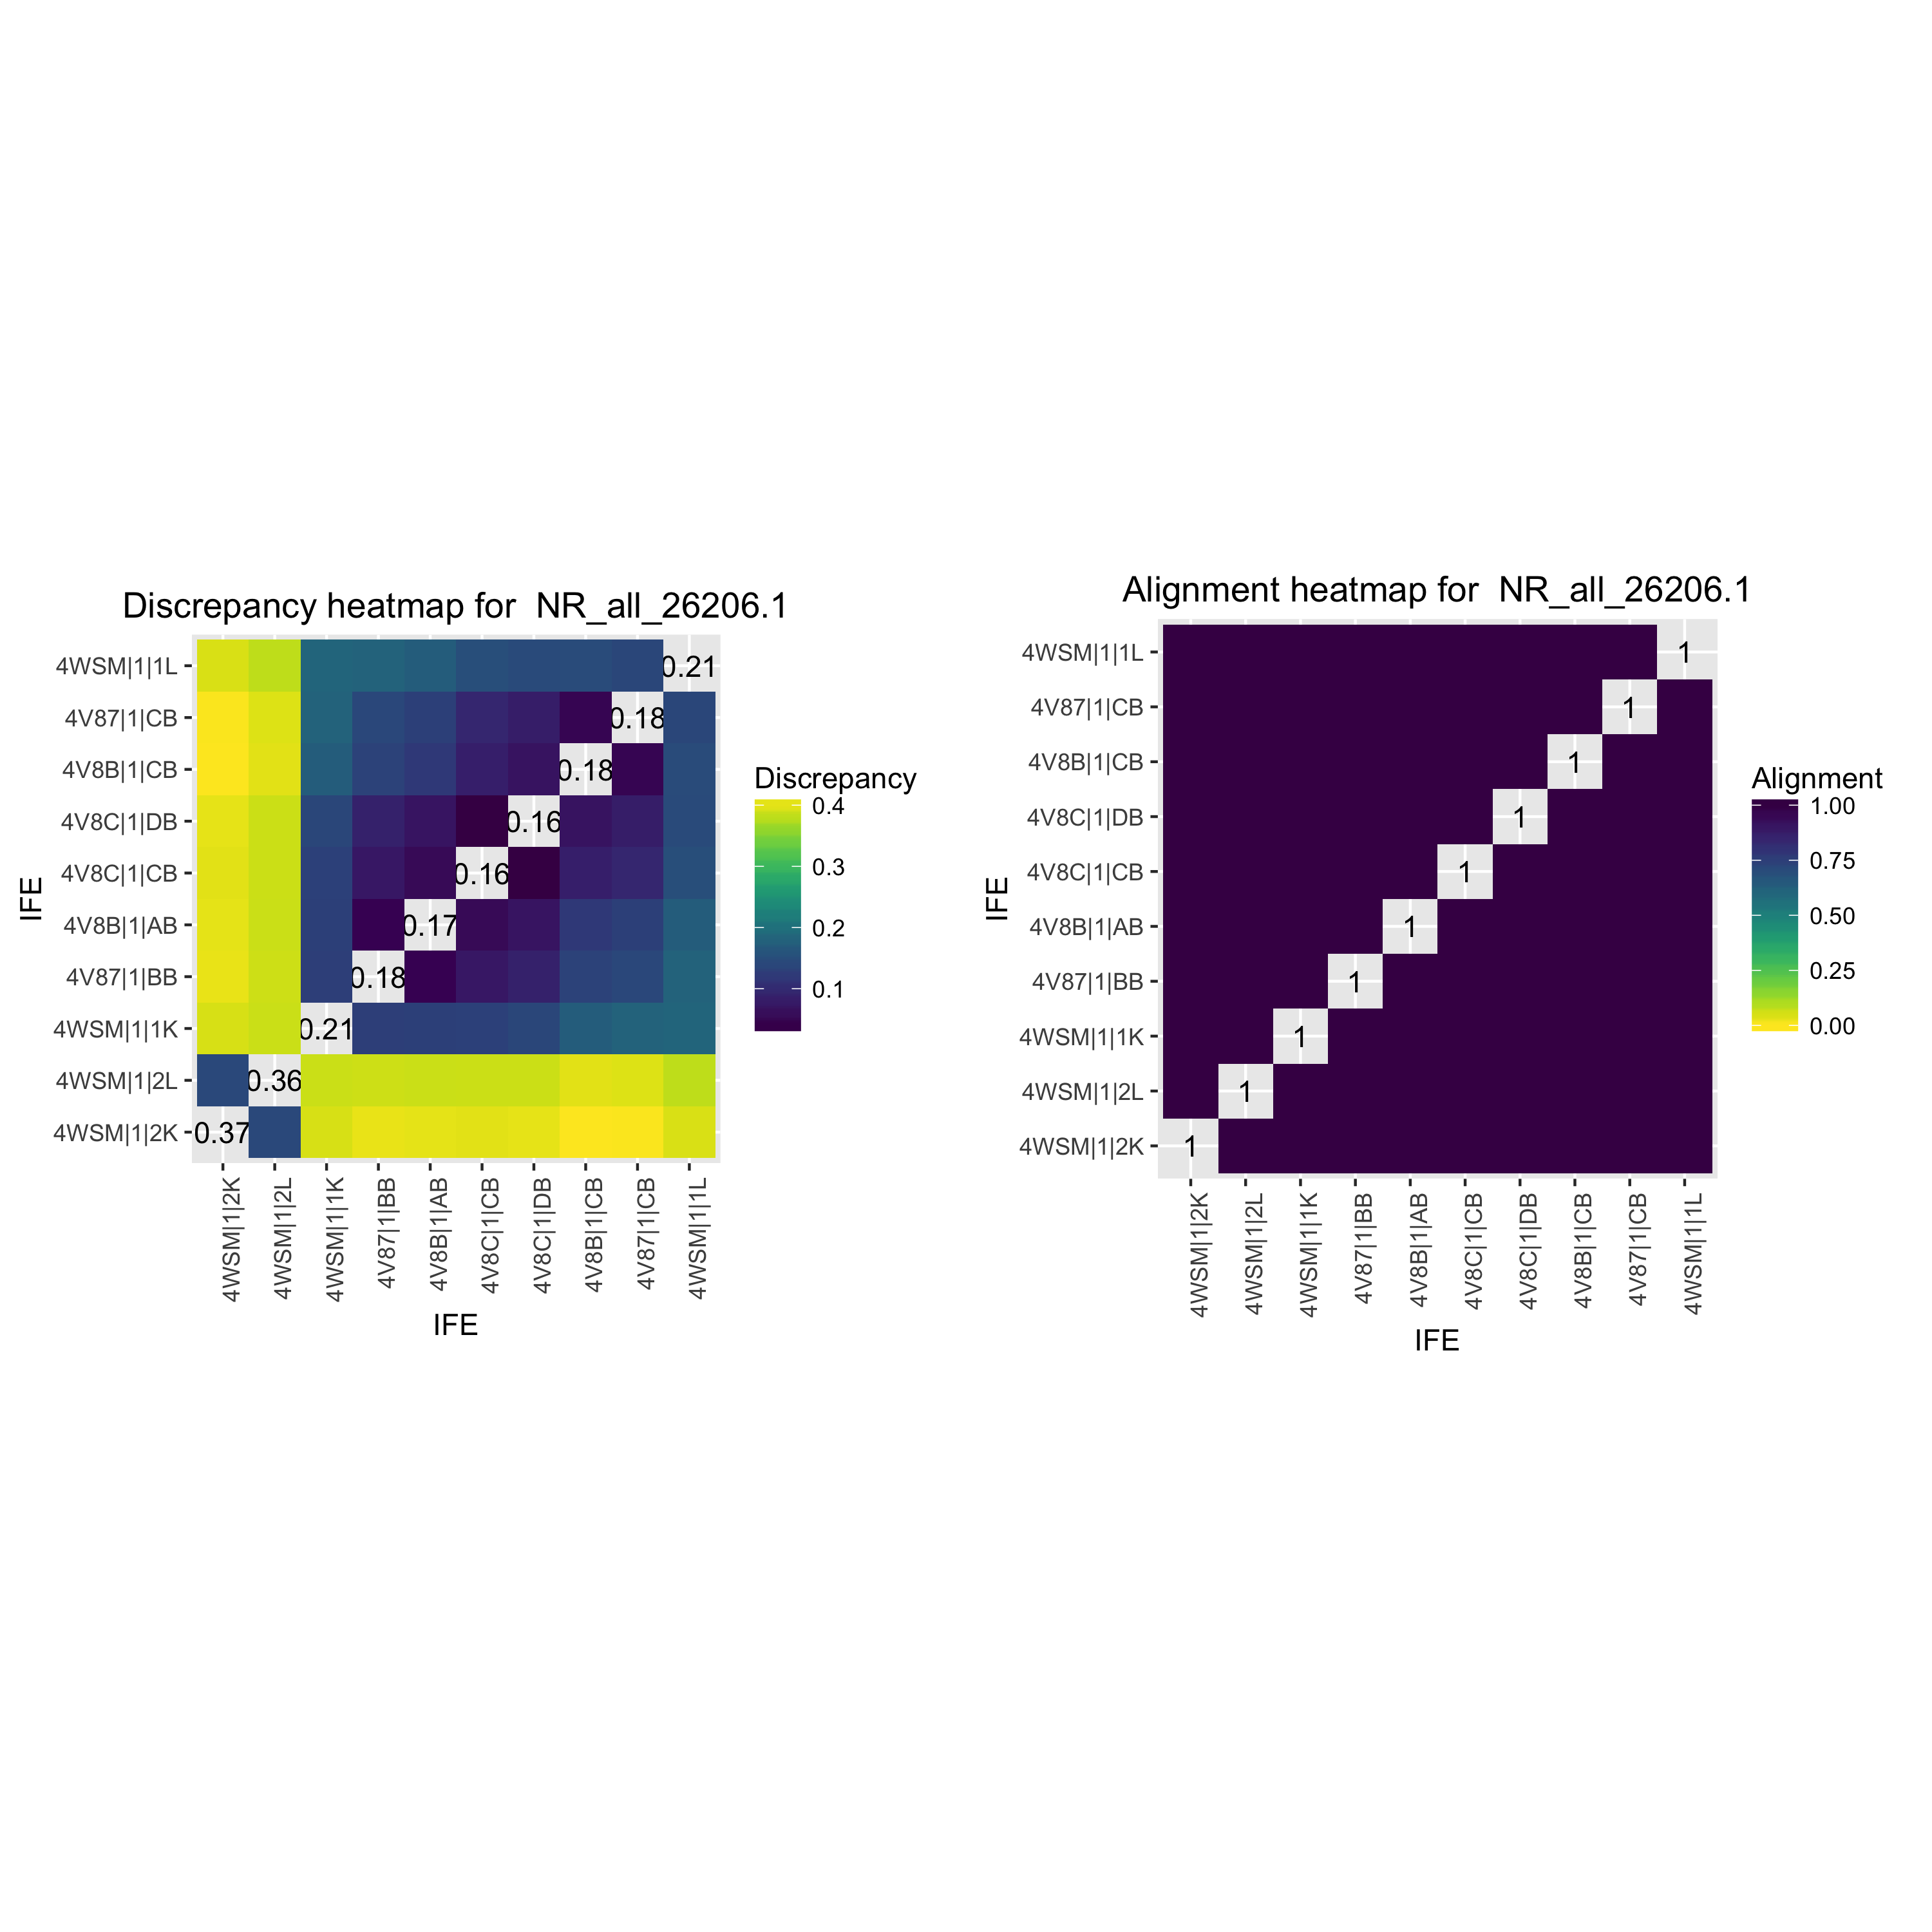
\includegraphics[width=\textwidth]{chapter-3/figs/trna-alone}
  \caption{Example of a tRNA/mRNA complex forming an equivalence class. On the
    left is a heat map of the discrepancies for all IFE’s in the group. The
    right shows the heat map of sequence similarity for the group. Color scales
    indicate the value, with lighter colors meaning ‘worse’ values. Along the
  diagonal of each plot is the mean value for each row.}
  \label{fig:trna-alone}
\end{figure}

\subsection{Protein and RNA complexes}

Small RNA/protein complexes are the groups which are most affected by usage of
discrepancy. To test how our method works we built a grouping with and without
discrepancy. We used a small, 11 nt, poly-A chain as a test case. This molecule
adopts different conformations depending upon the environment. In 4JRD it forms
a non-canonical duplex, while in 1CVJ it forms a single strand bound to a
protein. Shown in Figure~\ref{fig:small-aa-no-disc} we can see the discrepancy
of such a clustering. It contains several subgroups that are only connected
because we have not use discrepancy to split them. Upon using discrepancy this
group is partitioned into 4 other groups, one of which is shown in
Figure~\ref{fig:small-aa-disc}.  In this heatmap we can see that the group is
much more homogeneous and all pairs have discrepancy less than 0.2{\AA}/nt. In
addition all members of this group form a similar structure and are bound to
proteins, unlike the previous method where the group was a mix of single and
double stranded molecules.

\begin{figure}[h]
  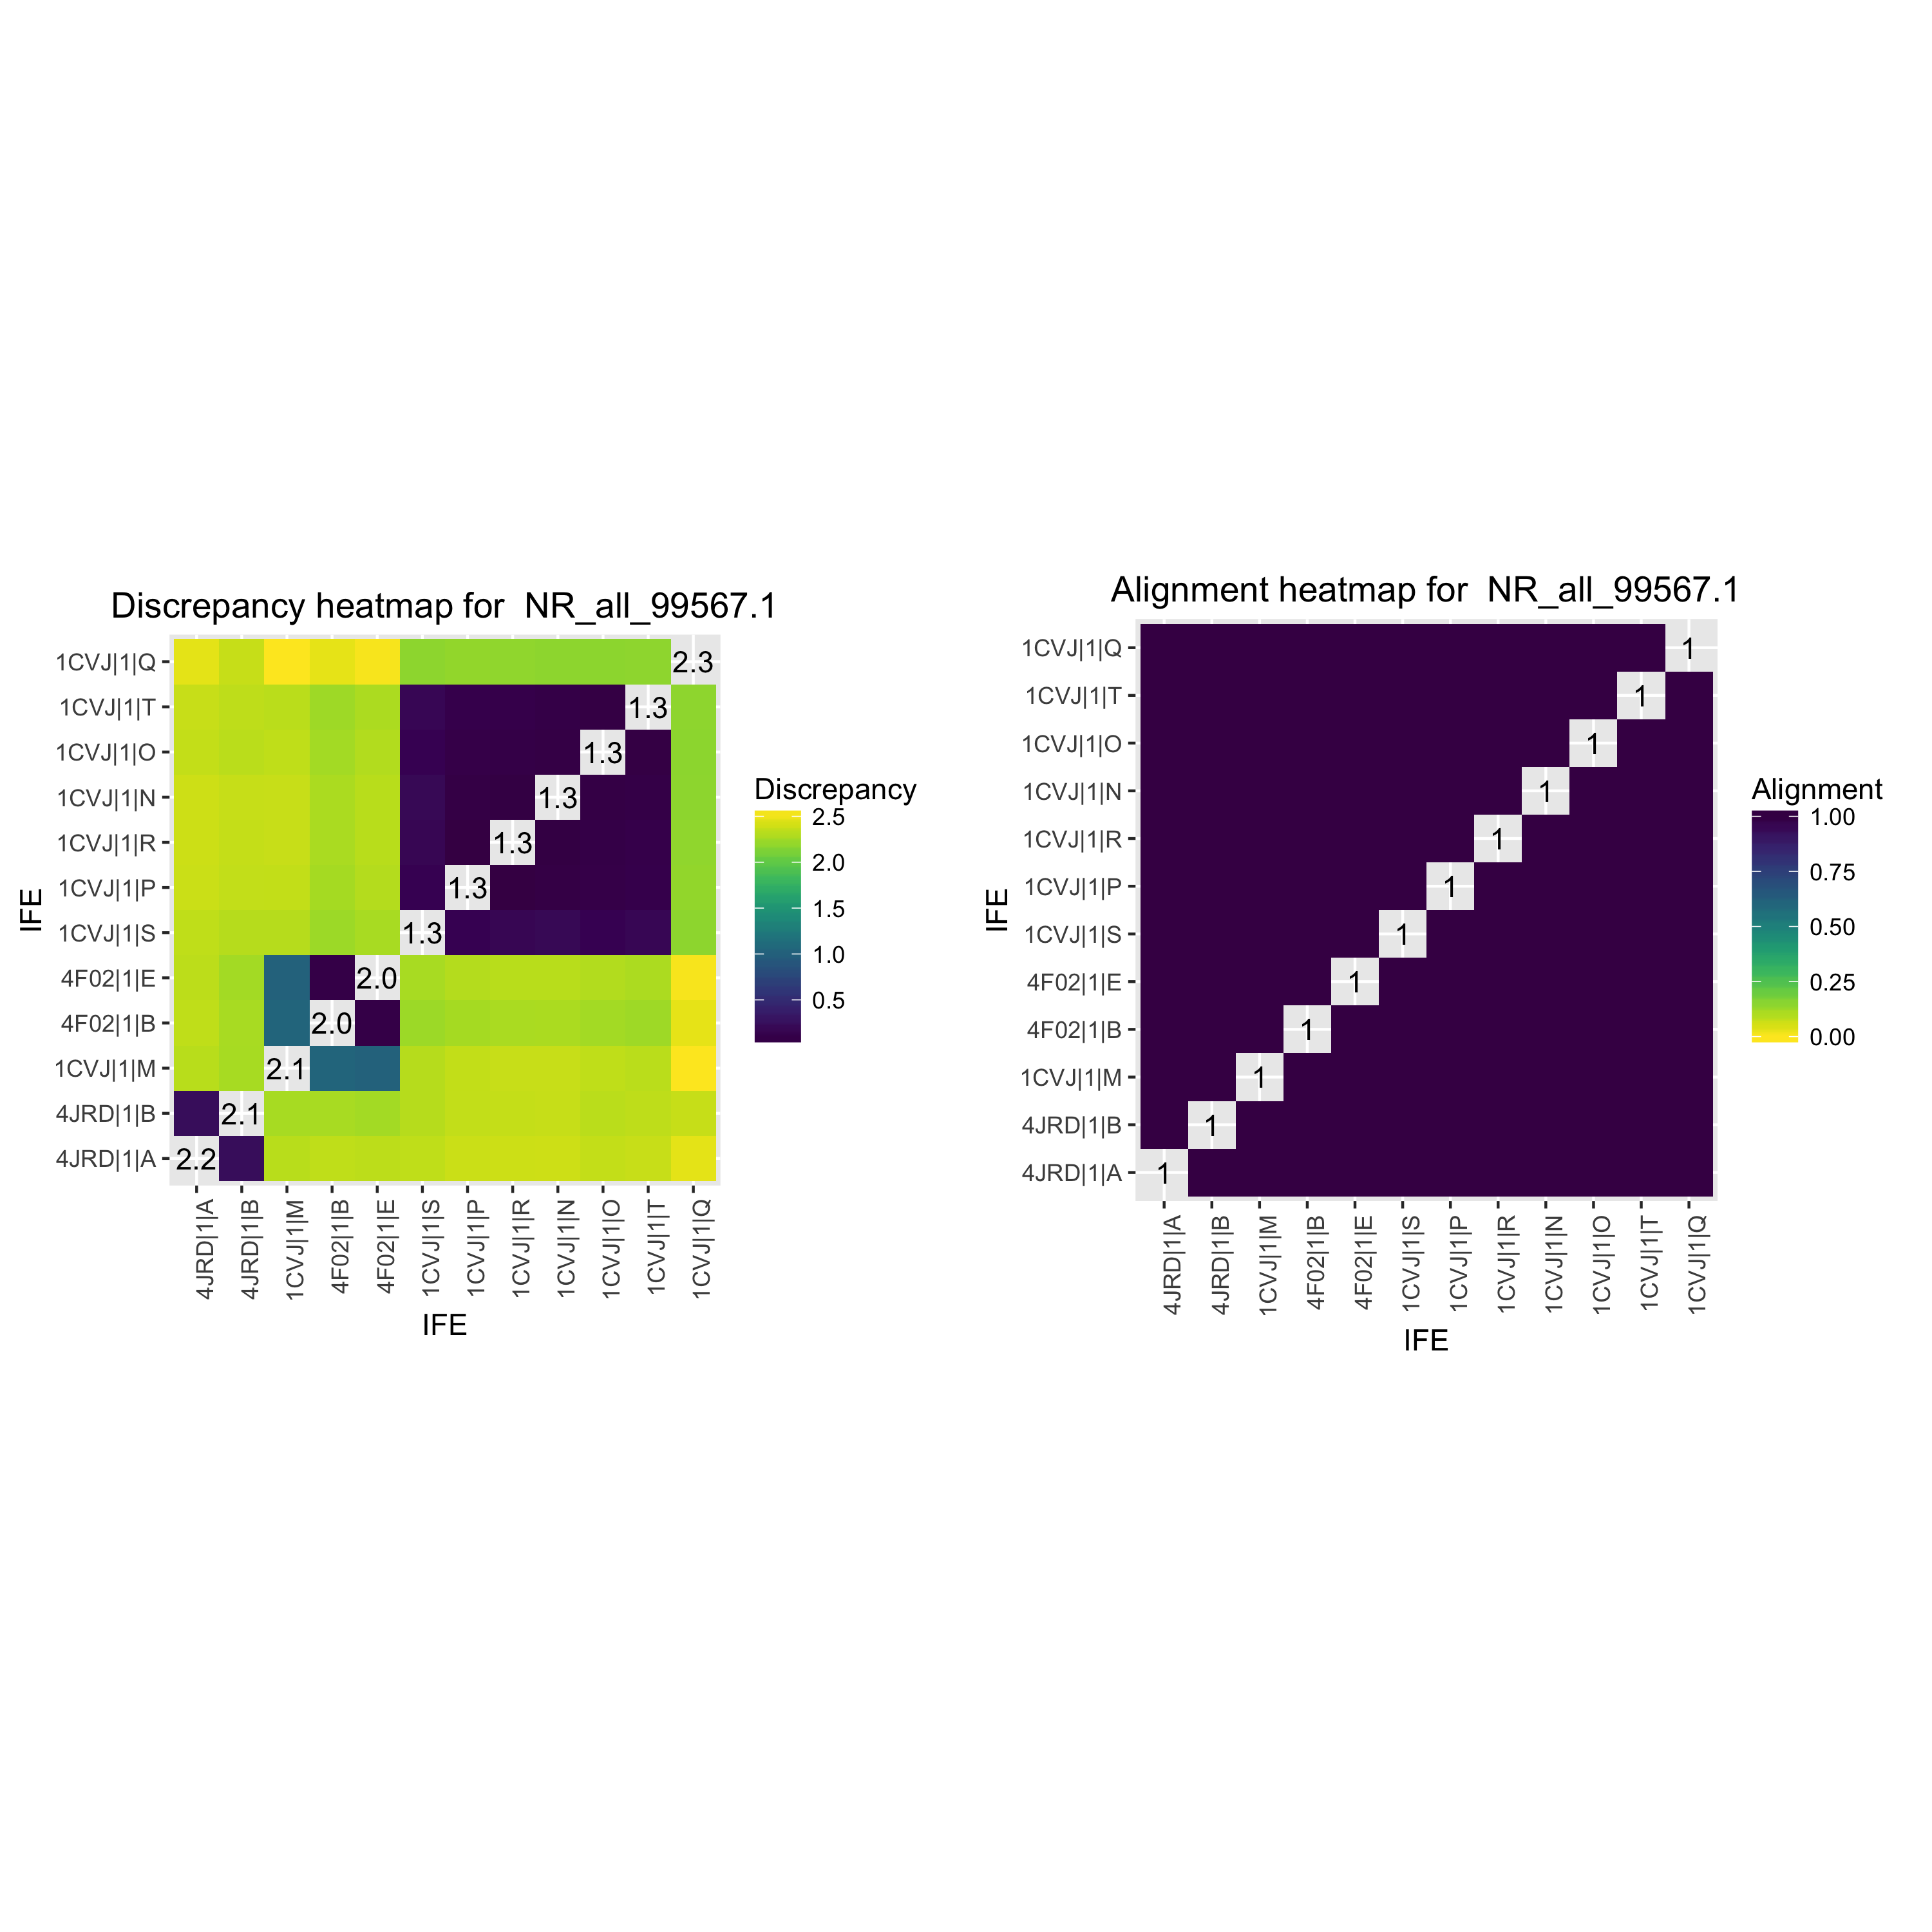
\includegraphics[width=\textwidth]{chapter-3/figs/small-aa-no-disc}
  \caption{Discrepancy heatmap for an 11-nt poly-A class built without
    discrepancy: This shows the effect of clustering a model compound without
    using discrepancy. We are showing only the discrepancy heatmap here. We can
  see that there are several subgroups with very different geometries.}
  \label{fig:small-aa-no-disc}
\end{figure}

\begin{figure}[h]
  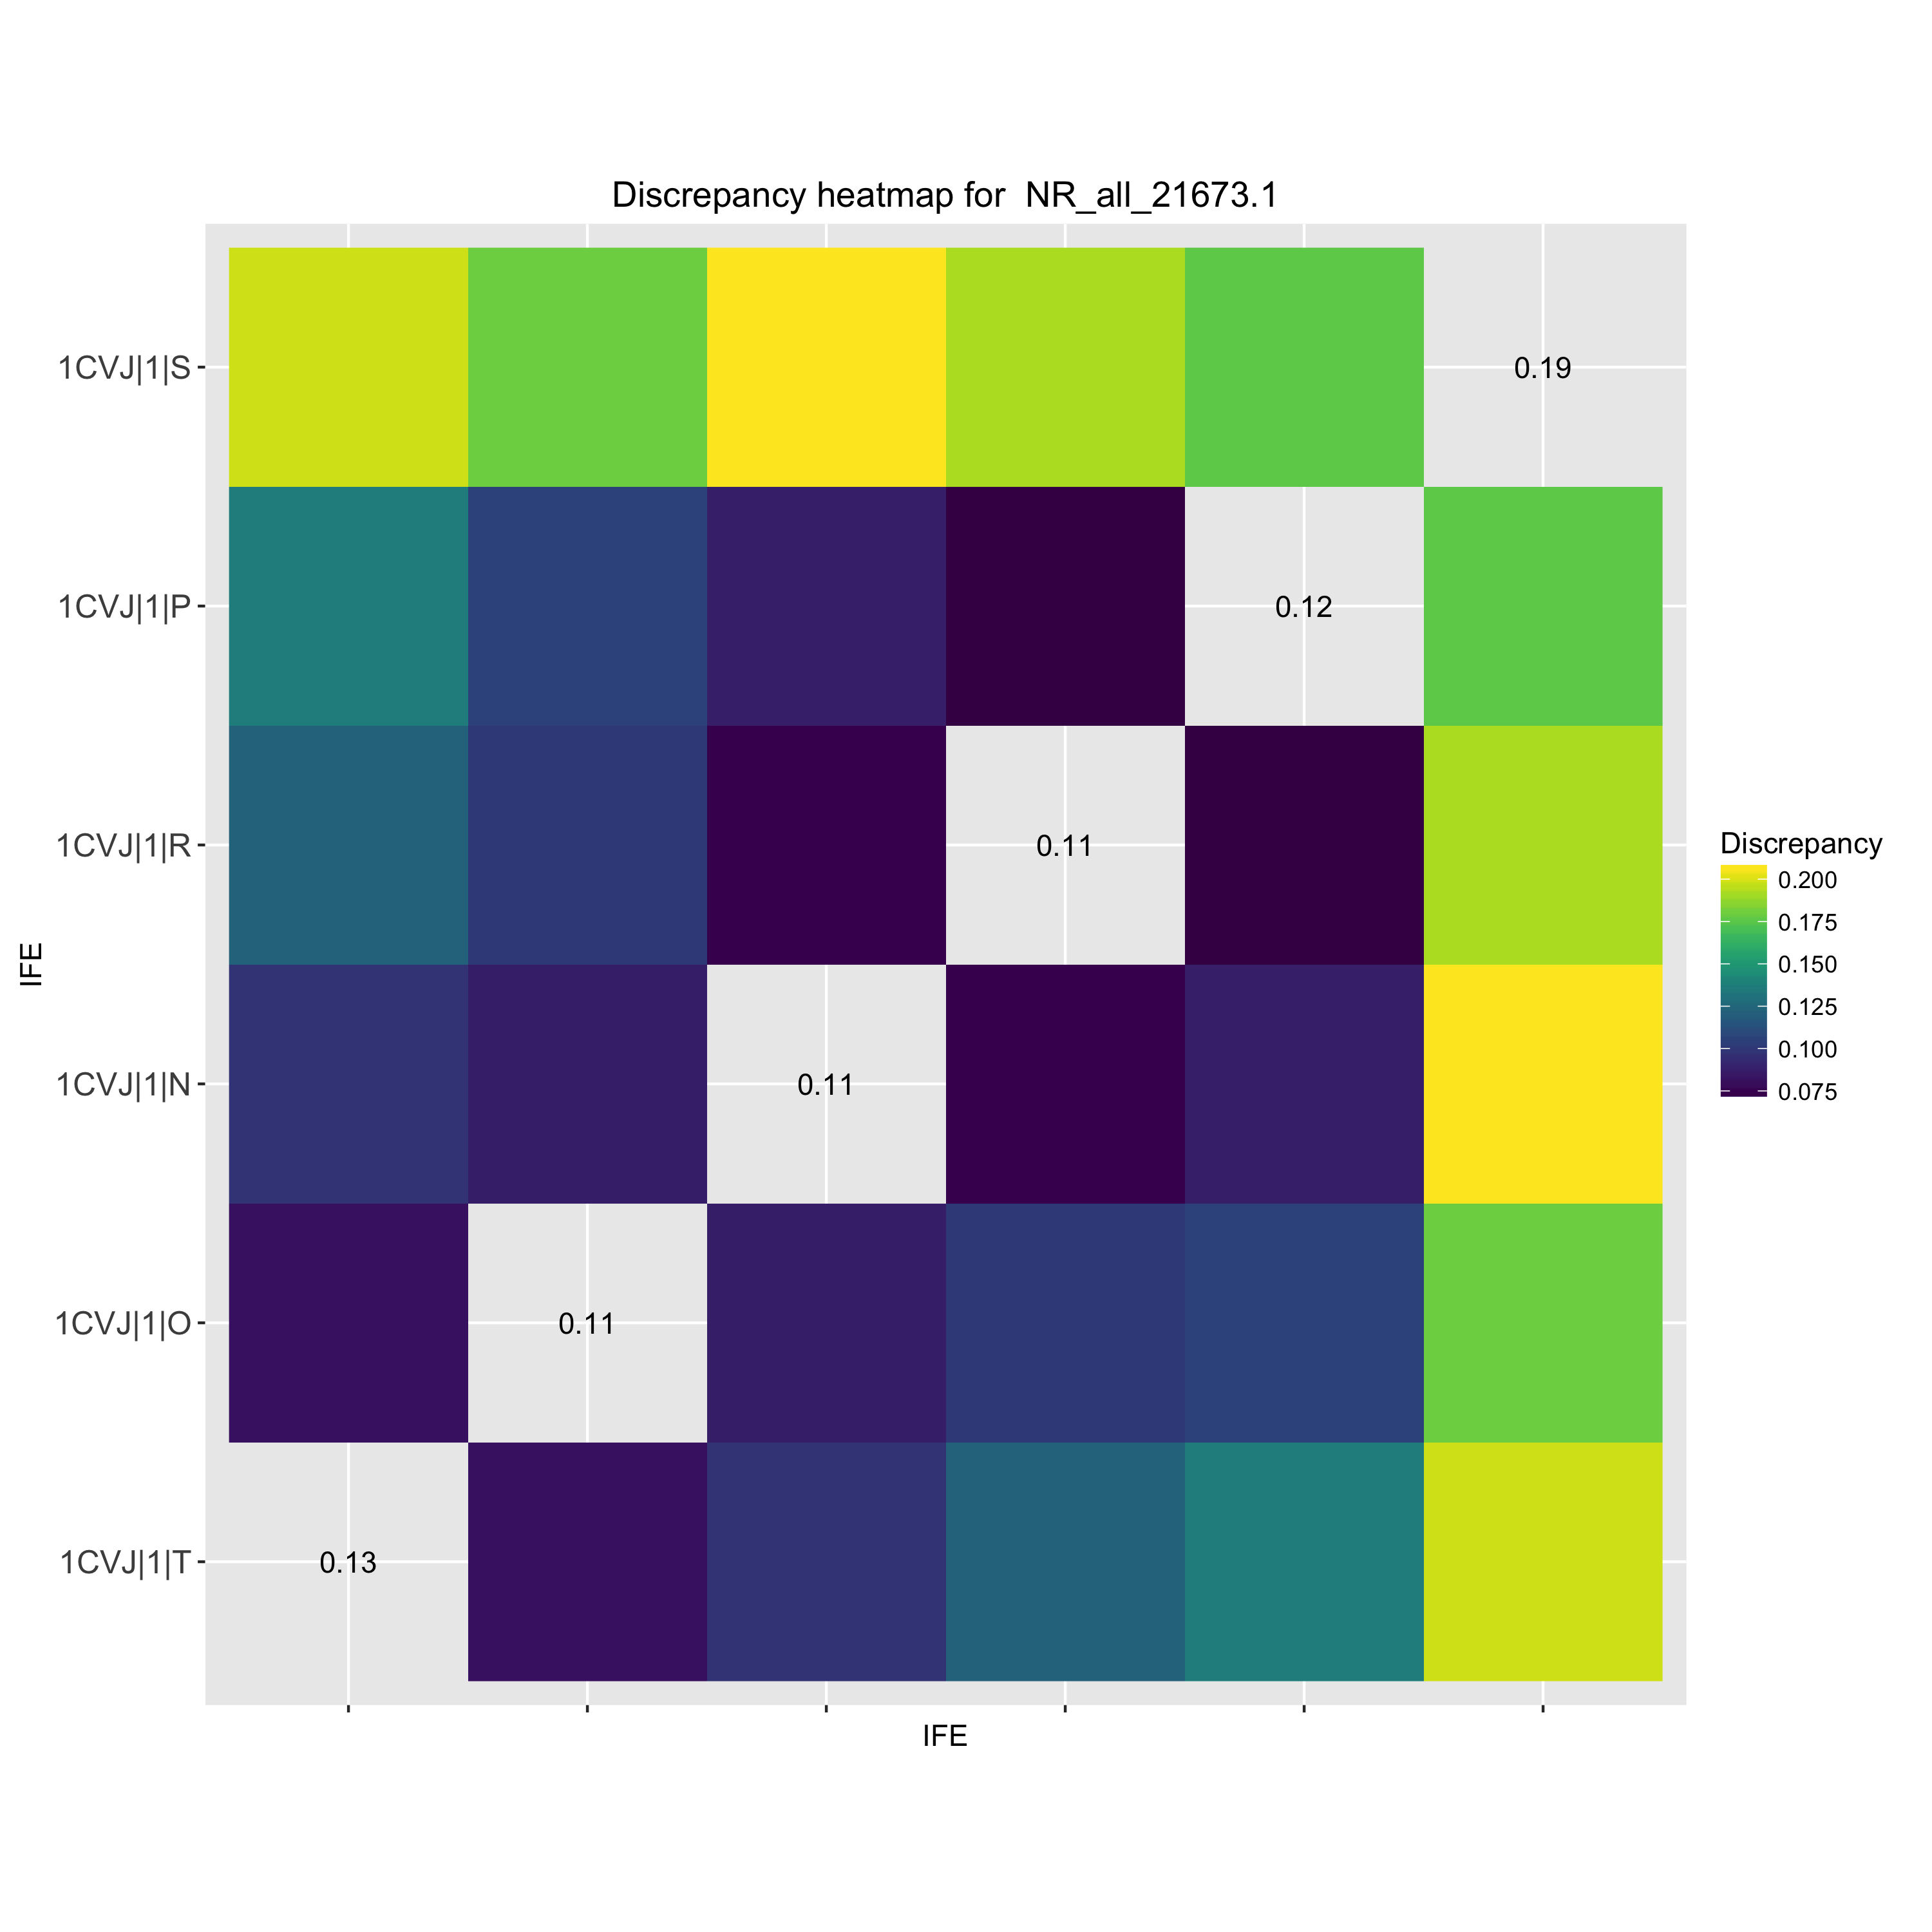
\includegraphics[width=\textwidth]{chapter-3/figs/small-aa-disc}
  \caption{Discrepancy heatmap for a small 11-nt poly-A compound built using
    discrepancy. Mean values for each row are shown on the diagonal, and the
  color scale indicates discrepancy with lighter colors being worse}
  \label{fig:small-aa-disc}
\end{figure}

\subsection{Outliers}

After evaluating specific cases we searched for outliers in our dataset. We
began by examining the distribution of maximum discrepancy and minimum sequence
similarity for all pairs in all equivalence classes. This is shown in in
Figure~\ref{fig:eq-summary}. From this figure we can see that most groups have a low
discrepancy and high sequence similarity. However, there is a very long tail of
groups with high discrepancies, some even ranging up to 4{\AA}/nt. This indicates
that some groups contain pairs of IFE's that are highly dissimilar. We call
these pairs outliers. For the purpose of this analysis we will define groups
with outliers as groups that contain pairs of IFE's with discrepancies greater
than 0.8{\AA}/nt or any group that contains a pair of IFE's that do not have a
‘good’ alignment. As discussed earlier, our criteria for chains to align well
depends on the size of the chains. For this reason we cannot use a simple
sequence similarity cutoff as with discrepancy.

\begin{figure}[h]
  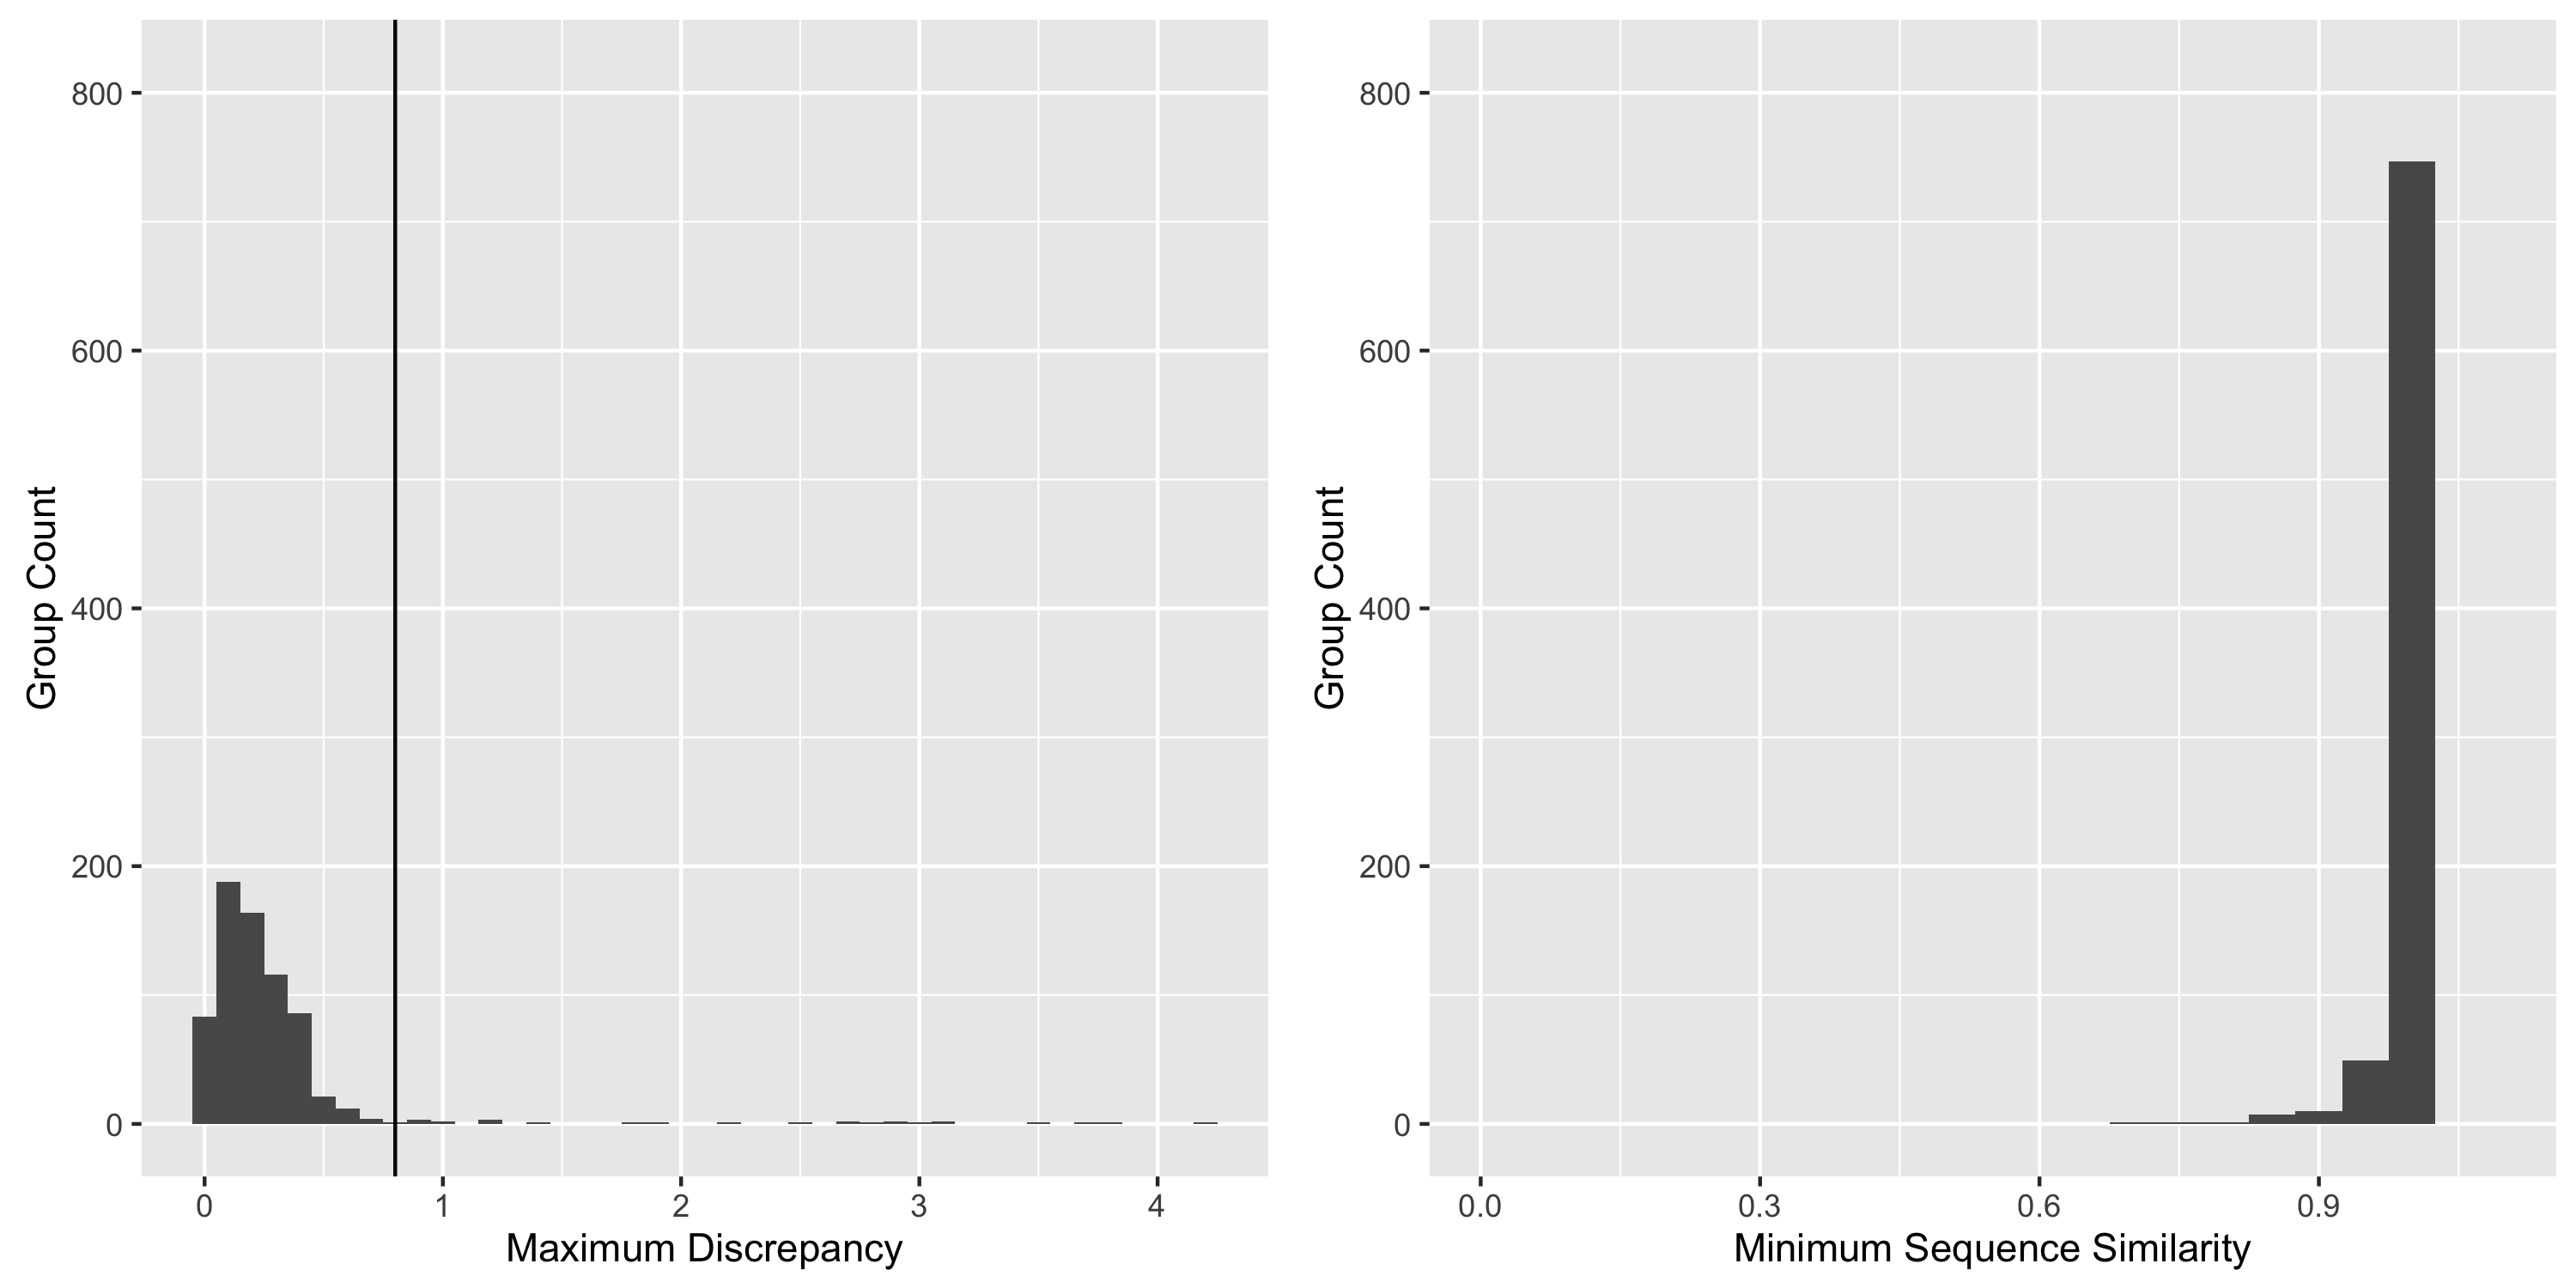
\includegraphics[width=\textwidth]{chapter-3/figs/eq-summary}
  \caption{A figure of the Maximum Pairwise Discrepancy and Minimum Sequence
    Similarity for all pairs of IFE's in all equivalence classes. The black
    lines indicate the 0.8 discrepancy cutoff (left) used a criterion for
  detecting groups with outlier pairs.}
  \label{fig:eq-summary}
\end{figure}

We then investigated the distribution of discrepancies and sequence similarities
for all groups containing outliers. The figuring summarizing this is shown in
Figure~\ref{fig:eq-outlier-summary}. This graph shows that outliers appear in all regions of
the graph. Some outliers have low discrepancy, indicating they must differ in
sequence, while others have high sequence similarity indicating they must differ
geometrically.

\begin{figure}[h]
  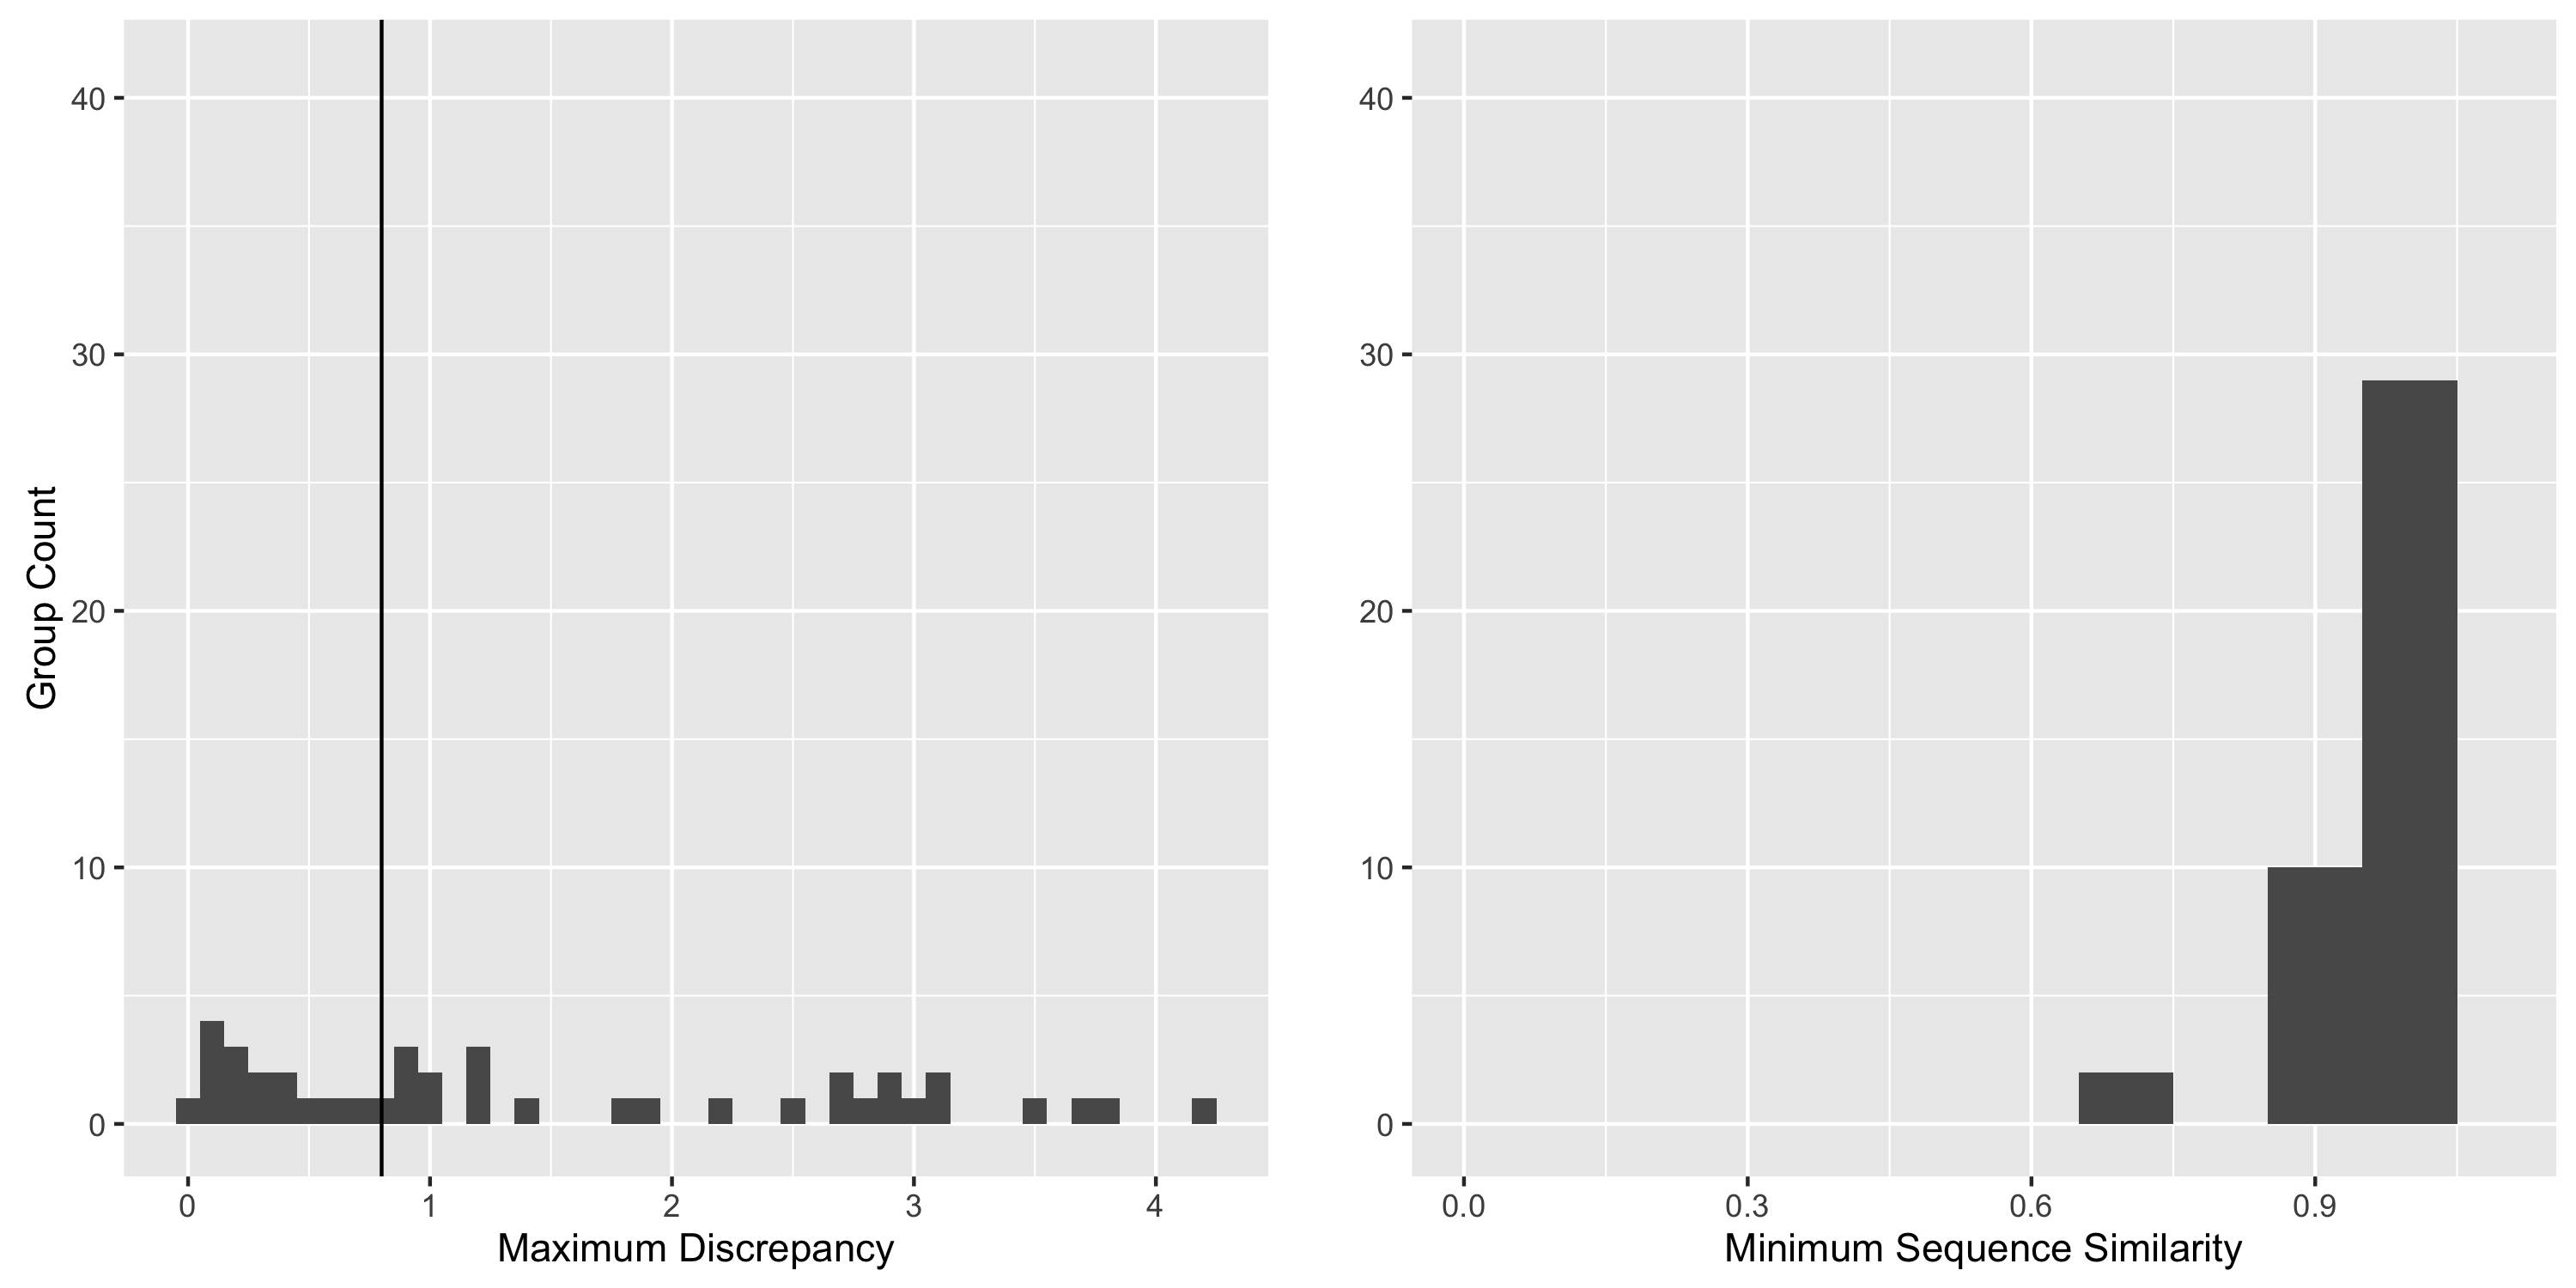
\includegraphics[width=\textwidth]{chapter-3/figs/outlier-summary}
  \caption{Discrepancy and Minimum Sequence Similarity of all groups with
  outliers. This figure shows the same data as Figure~\ref{fig:eq-summary} but
only for groups that have a pair of IFE's with discrepancy at least 0.8 or
sequence similarity less than or equal to 0.9.}
  \label{fig:eq-outlier-summary}
\end{figure}

We next examined the distribution of the number outliers, fraction of outliers,
discrepancy, and sequence similarity with respect to the size of the group in
terms of nucleotides and members as shown in Figure~\ref{fig:outlier-detail}.
This figure shows that the majority of the groups with outliers contain
relatively few members and are relatively small. However, there are a few groups
that contain many members and are large. The spike at \~80 nucleotides
corresponds to 2 tRNA groups.

\begin{figure}[h]
  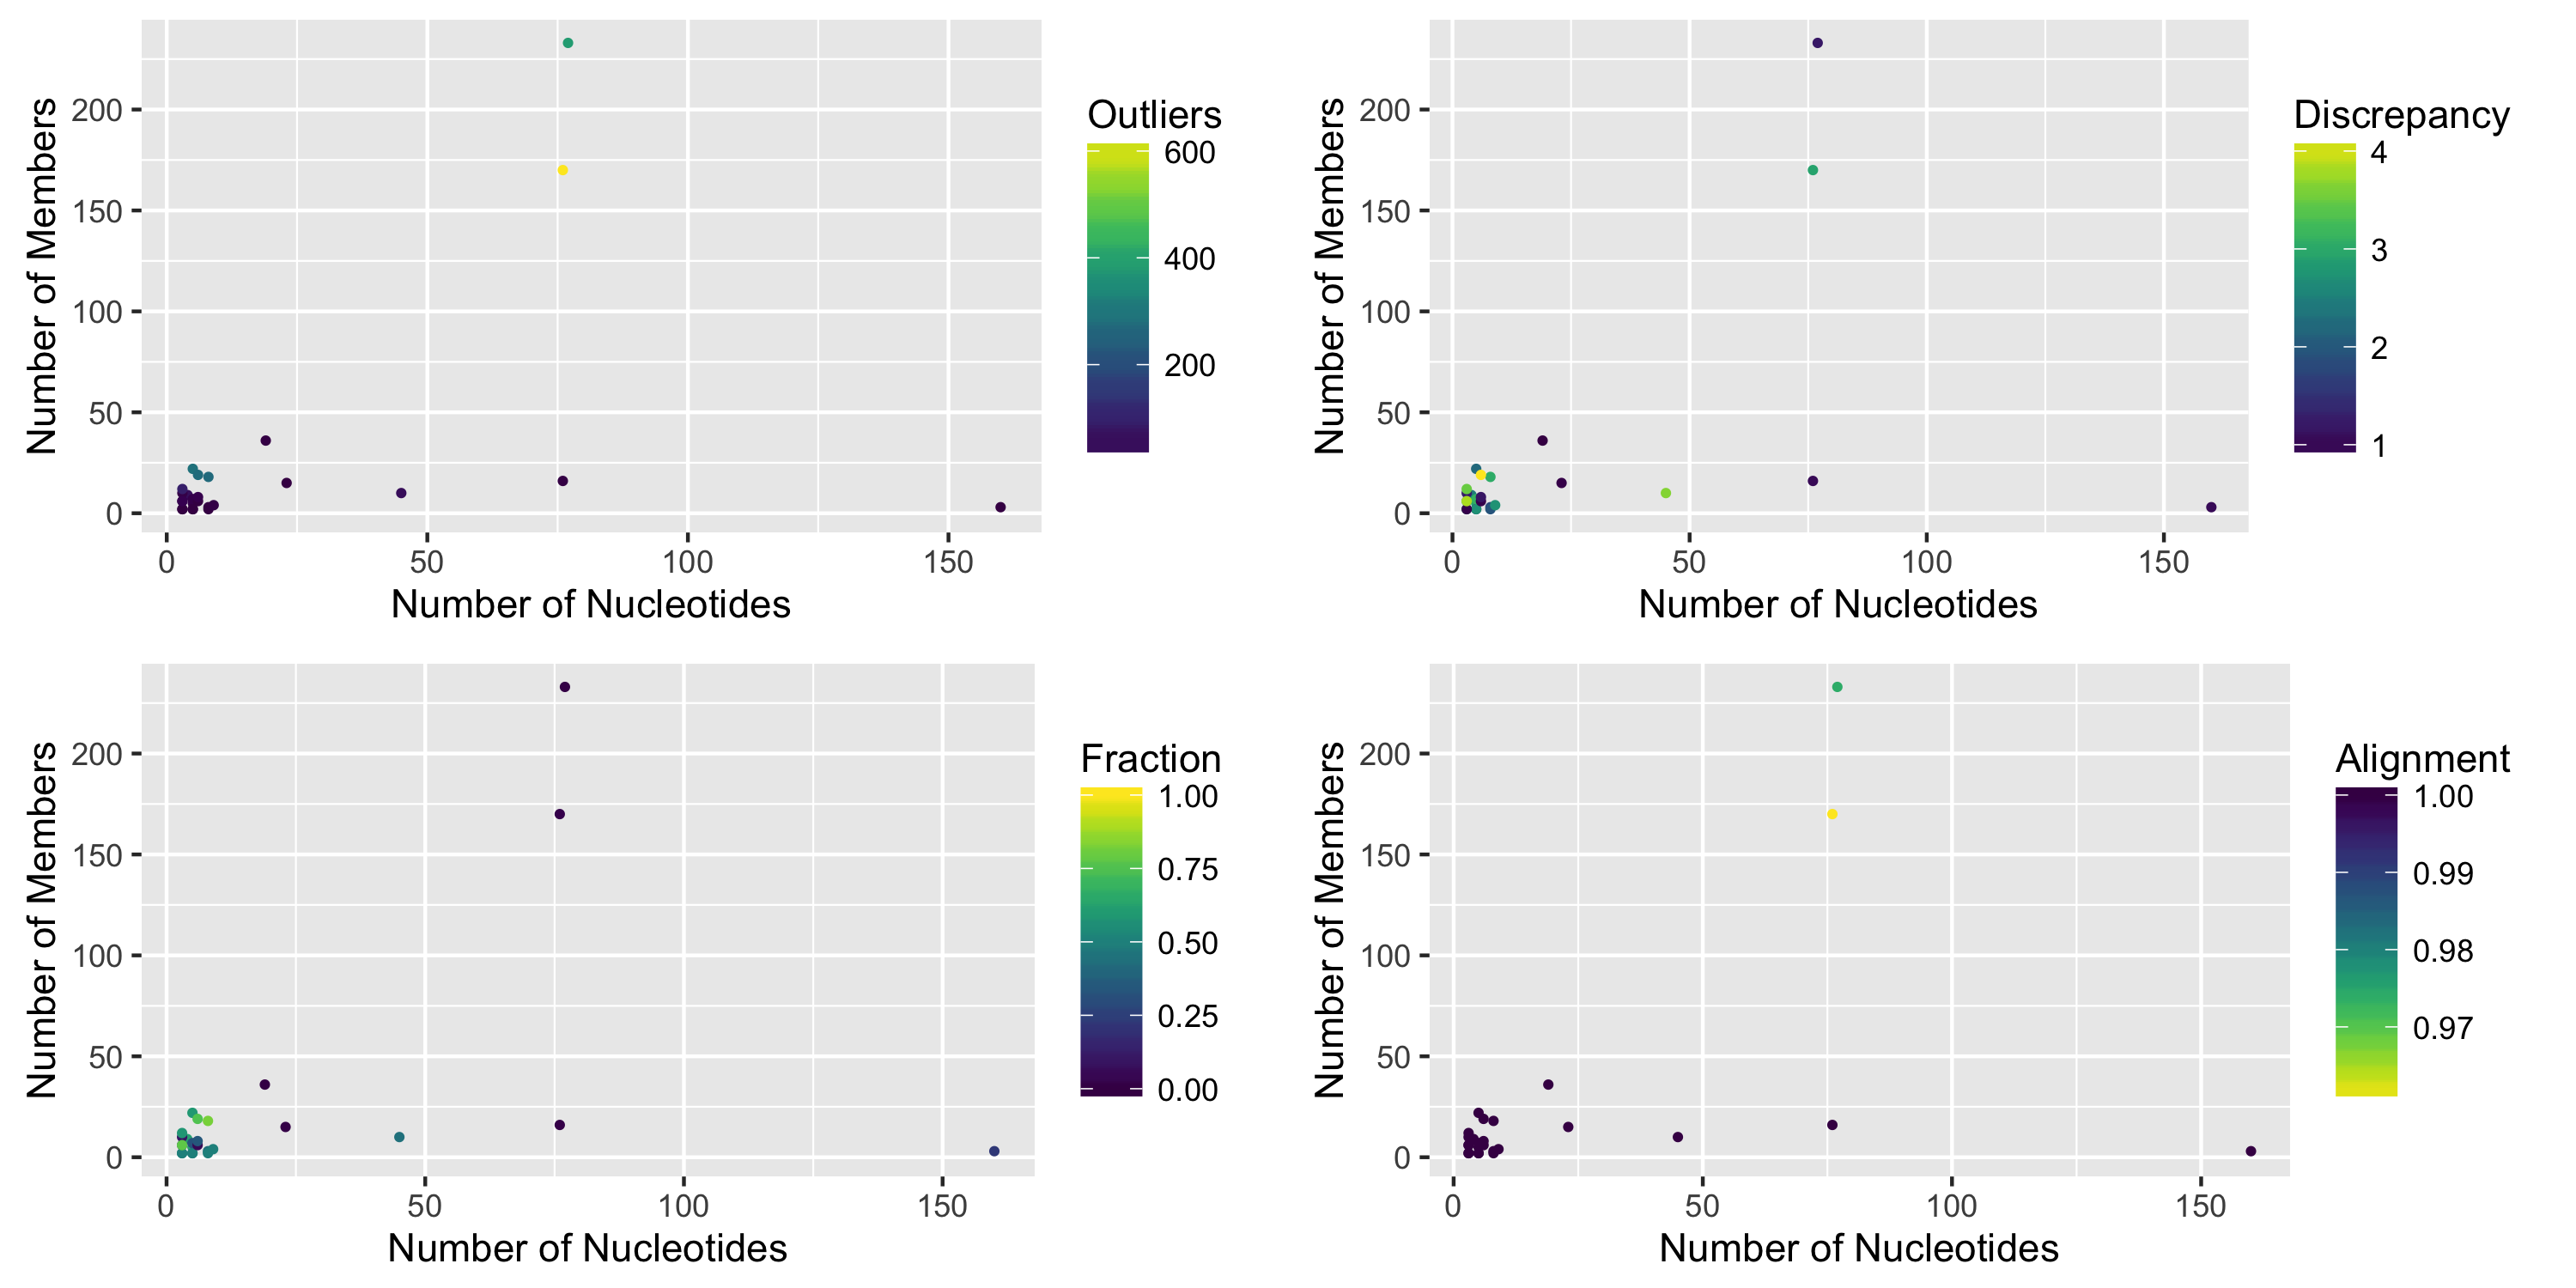
\includegraphics[width=\textwidth]{chapter-3/figs/outlier-details}
  \caption{This figure shows 4 different metrics for outliers within each group.
    Each point in all graphs represents a group that contains at least one pair
    of IFE’s that is an outlier (discrepancy greater than 0.8 or sequence
    similarity less than 0.9). In all graphs the horizontal coordinate is the
    number of nucleotides in the representative (discussed in the next chapter)
    of the group. The vertical is the number of members. The points are colored
    according to various metrics. In the upper right the points are colored
    using the number of pairs that are outliers, with lighter colors meaning
    more. Proceeding clockwise to the upper right the points are colored
    according to the the maximum discrepancy amongst all pairs in the groups.
    The lower right shows the minimum sequence similarity with lighter being a
    lower (worse) score. Finally, the lower left colors the points using the
    fraction of total pairs that are outliers, with lighter being higher
  fraction and thus worse.}
  \label{fig:outlier-detail}
\end{figure}

All groups with outliers can be classified according to the type of of outliers
they contain. The groups may contain pairs that have high discrepancy, low
sequence similarity or both high discrepancy and low sequence similarity. I
determined the counts for each of these as shown in
Table~\ref{tab:outlier-types}. This table shows that the majority of the groups,
63\%, have at least one pair with high discrepancy. The remaining 36\% of groups
contain pairs that have low sequence similarity and no pairs with high
discrepancy. I explored these classes to determine how such groups were built.

\begin{table}
  \begin{tabular}{lr}
    \toprule
    Outlier Type & Number of Groups (Percent) \\
    \midrule
    High Discrepancy & 21 (51\%) \\
    Low Sequence Similarity & 15 (36\%) \\
    High Discrepancy and Low Sequence Similarity & 5 (12\%) \\
    \bottomrule
  \end{tabular}
  \caption{This table shows the counts, and percents, of each type of outlier
  in an equivalence class.}
  \label{tab:outlier-types}
\end{table}

From the definition of our methodology, I know that all groups that contain
pairs with low sequence similarity will do so because they are connected through
a chain of high sequence similarity pairs. The NR\_all\_03381.1 group contains
protein/stem loop constructs of length 22 nt and has 4 members,
\ife{1K8W}{1}{B}, \ife{1ZL3}{1}{B}, \ife{1ZE2}{1}{D} , and 1ZE.

The other class of groups with outliers, those that contain a pair with high
discrepancy, can be caused in two ways. First, the pairs may be connected
through a chain of low discrepancies, similar to pairs with low sequence
similarity being connected through a chain of high sequence similarity pairs.
This is visible in Figure~\ref{fig:nr-all-75770.1-disc}. In this figure there are
yellow bars that only cover part of the

\begin{figure}[h]
  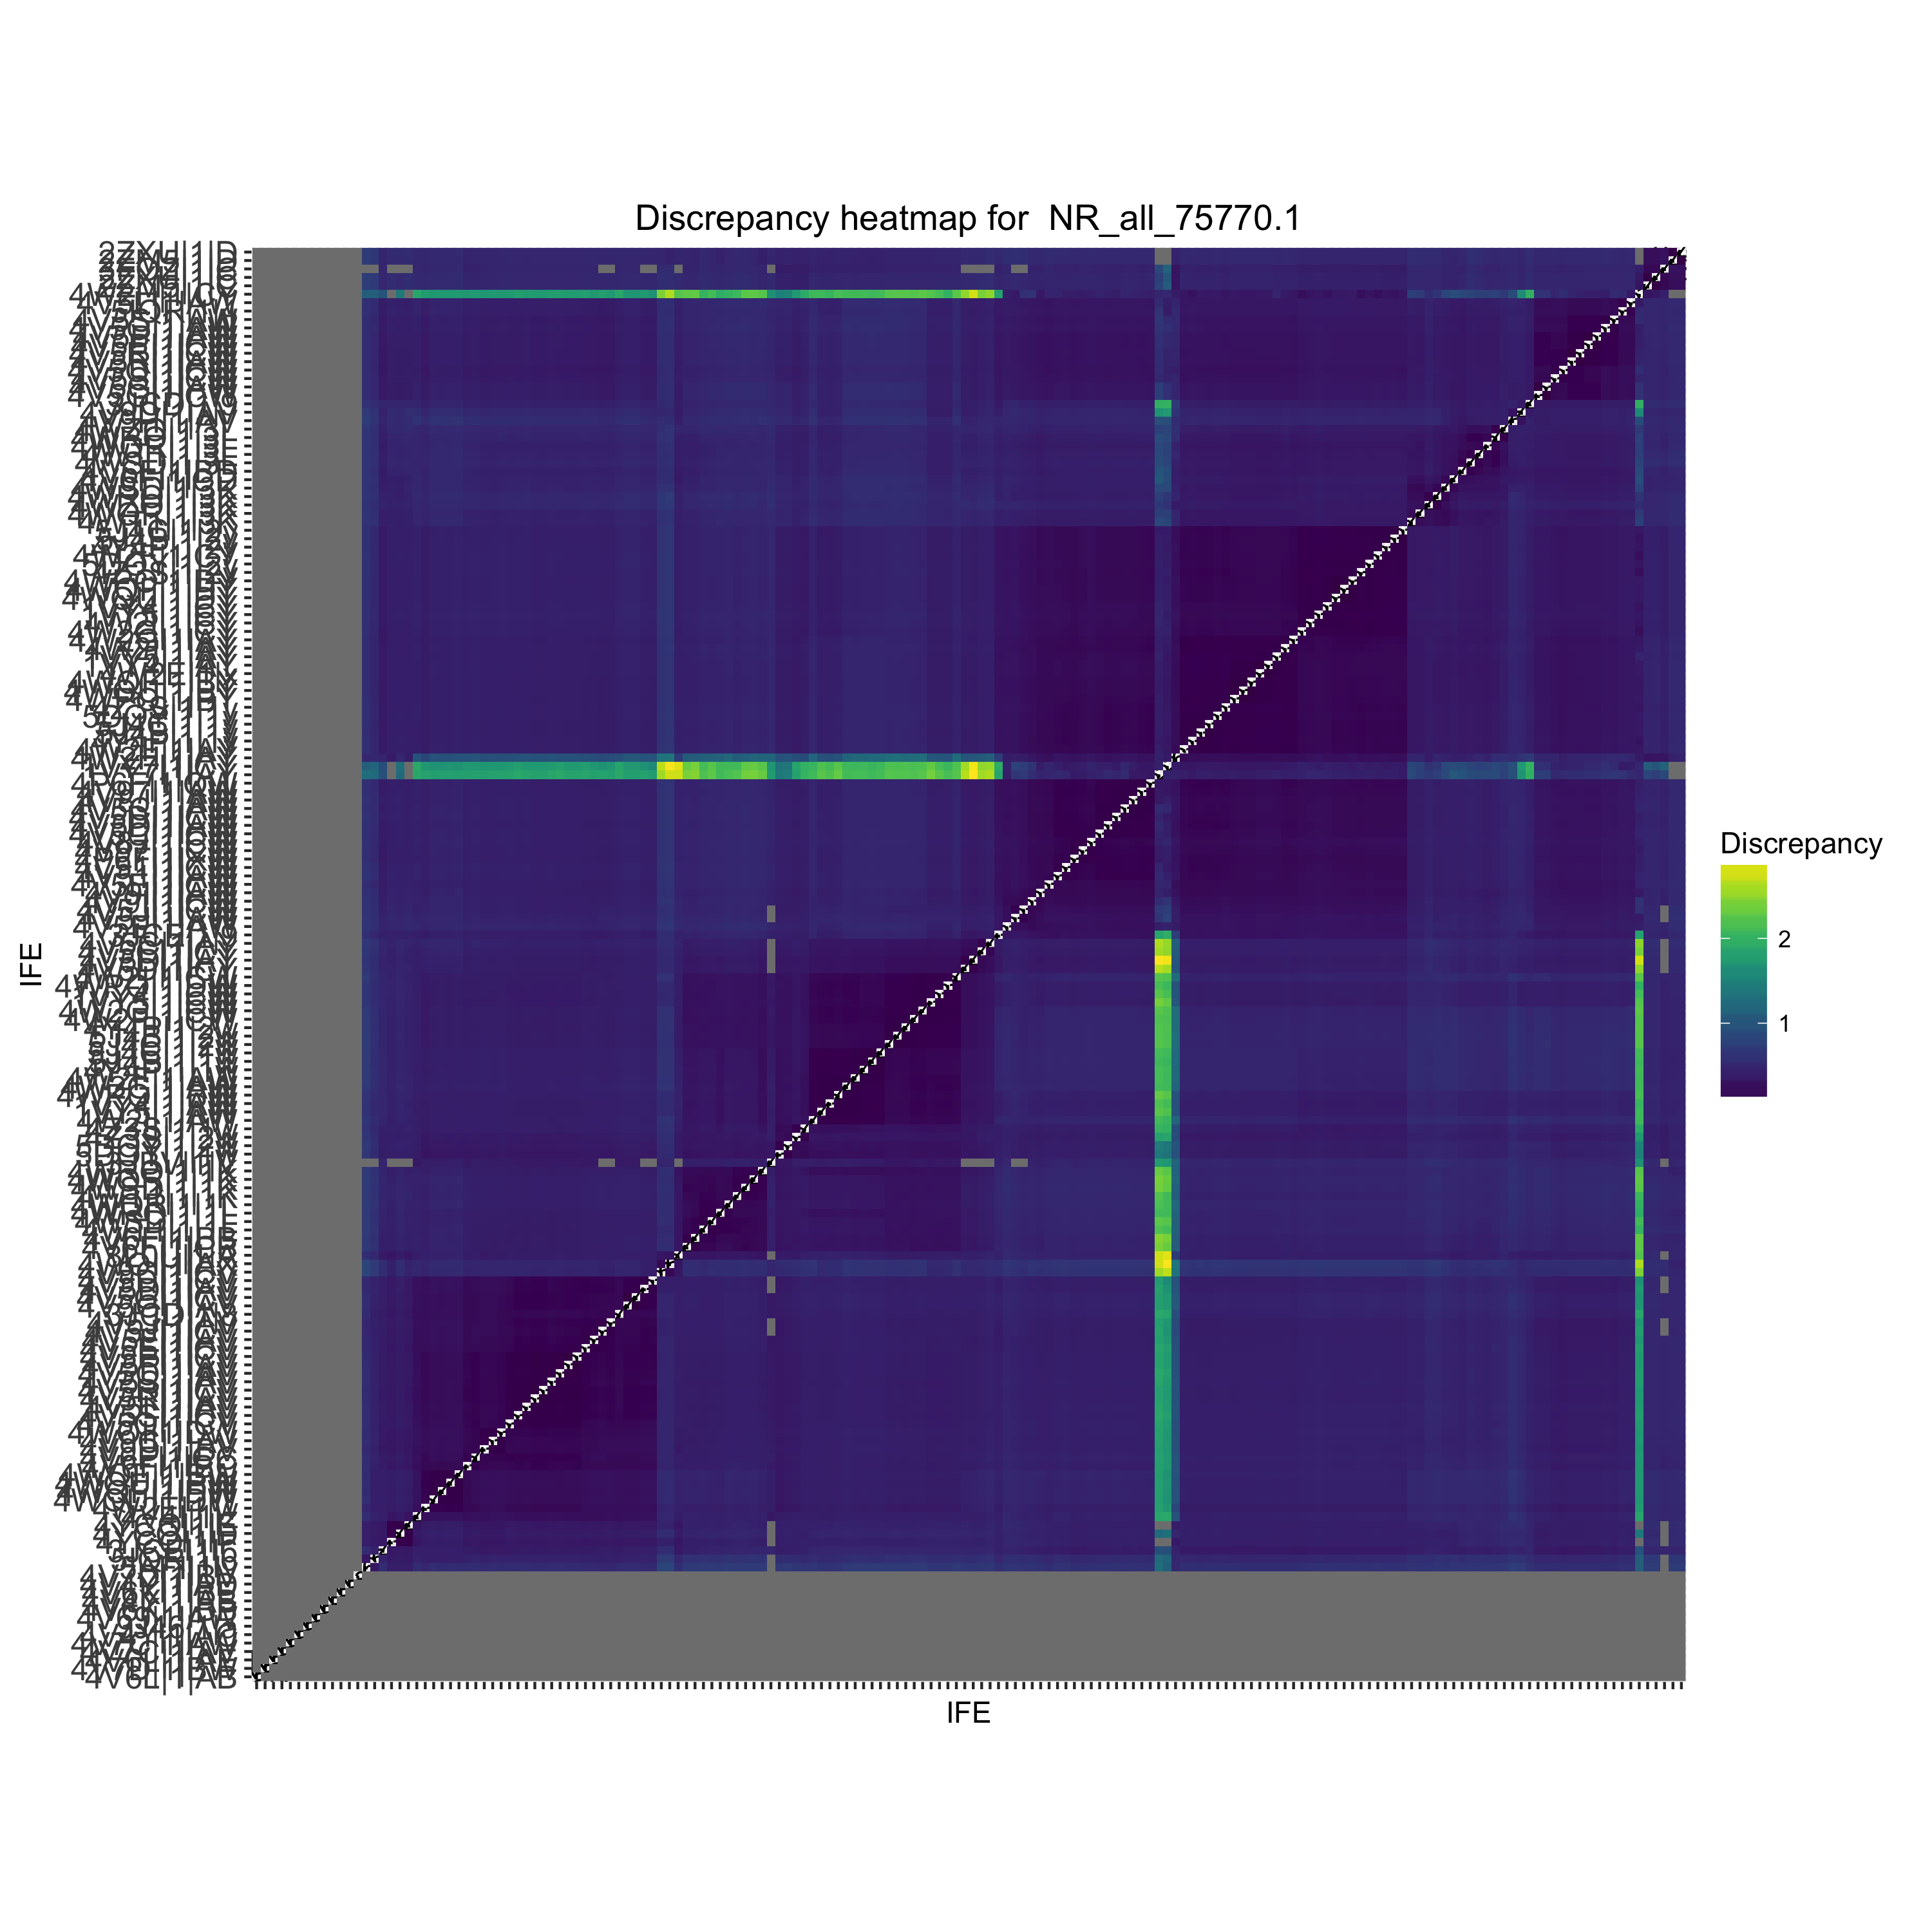
\includegraphics[width=\linewidth]{chapter-3/figs/nr-all-75770-1-disc}
  \caption{Histogram of the of the discrepancies for EC NR\_all\_75770.1, an E.
    coli tRNA group. This group contains a few IFE's which are outliers in our
  analysis.}
  \label{fig:nr-all-75770.1-disc}
\end{figure}

The other possibility is that the chains are connected through an IFE which did
not have discrepancy computed. An example of this is show in NR\_all\_18070.1
DISC. In this figure we can see a yellow line in the upper right which covers
the entire heatmap. This indicates that this IFE has high discrepancy to all
other members of the group. This IFE is connected to all other members through
the IFE’s that have no discrepancy shown (grey bars).

We examined the two groups, NR\_all\_18070.1 and NR\_all\_75770.1 manually and found
that they are tRNA groups. We will look at NR\_all\_18070.1 first, which is a tRNA
group with 233 members and is the highest point on the summary graphs. Shown in
Figure~\ref{fig:nr-all-18070.1-disc}. The outliers are due to a single IFE which is a
truncated tRNA. While it is somewhat structurally different from all other
members it is very similar in sequence. Because these molecules are uncommon and
it is still similar enough to rest of the group to ‘belong’. It is connected to
the rest of the chains through IFE’s which have no computed discrepancy.

\begin{figure}[h]
        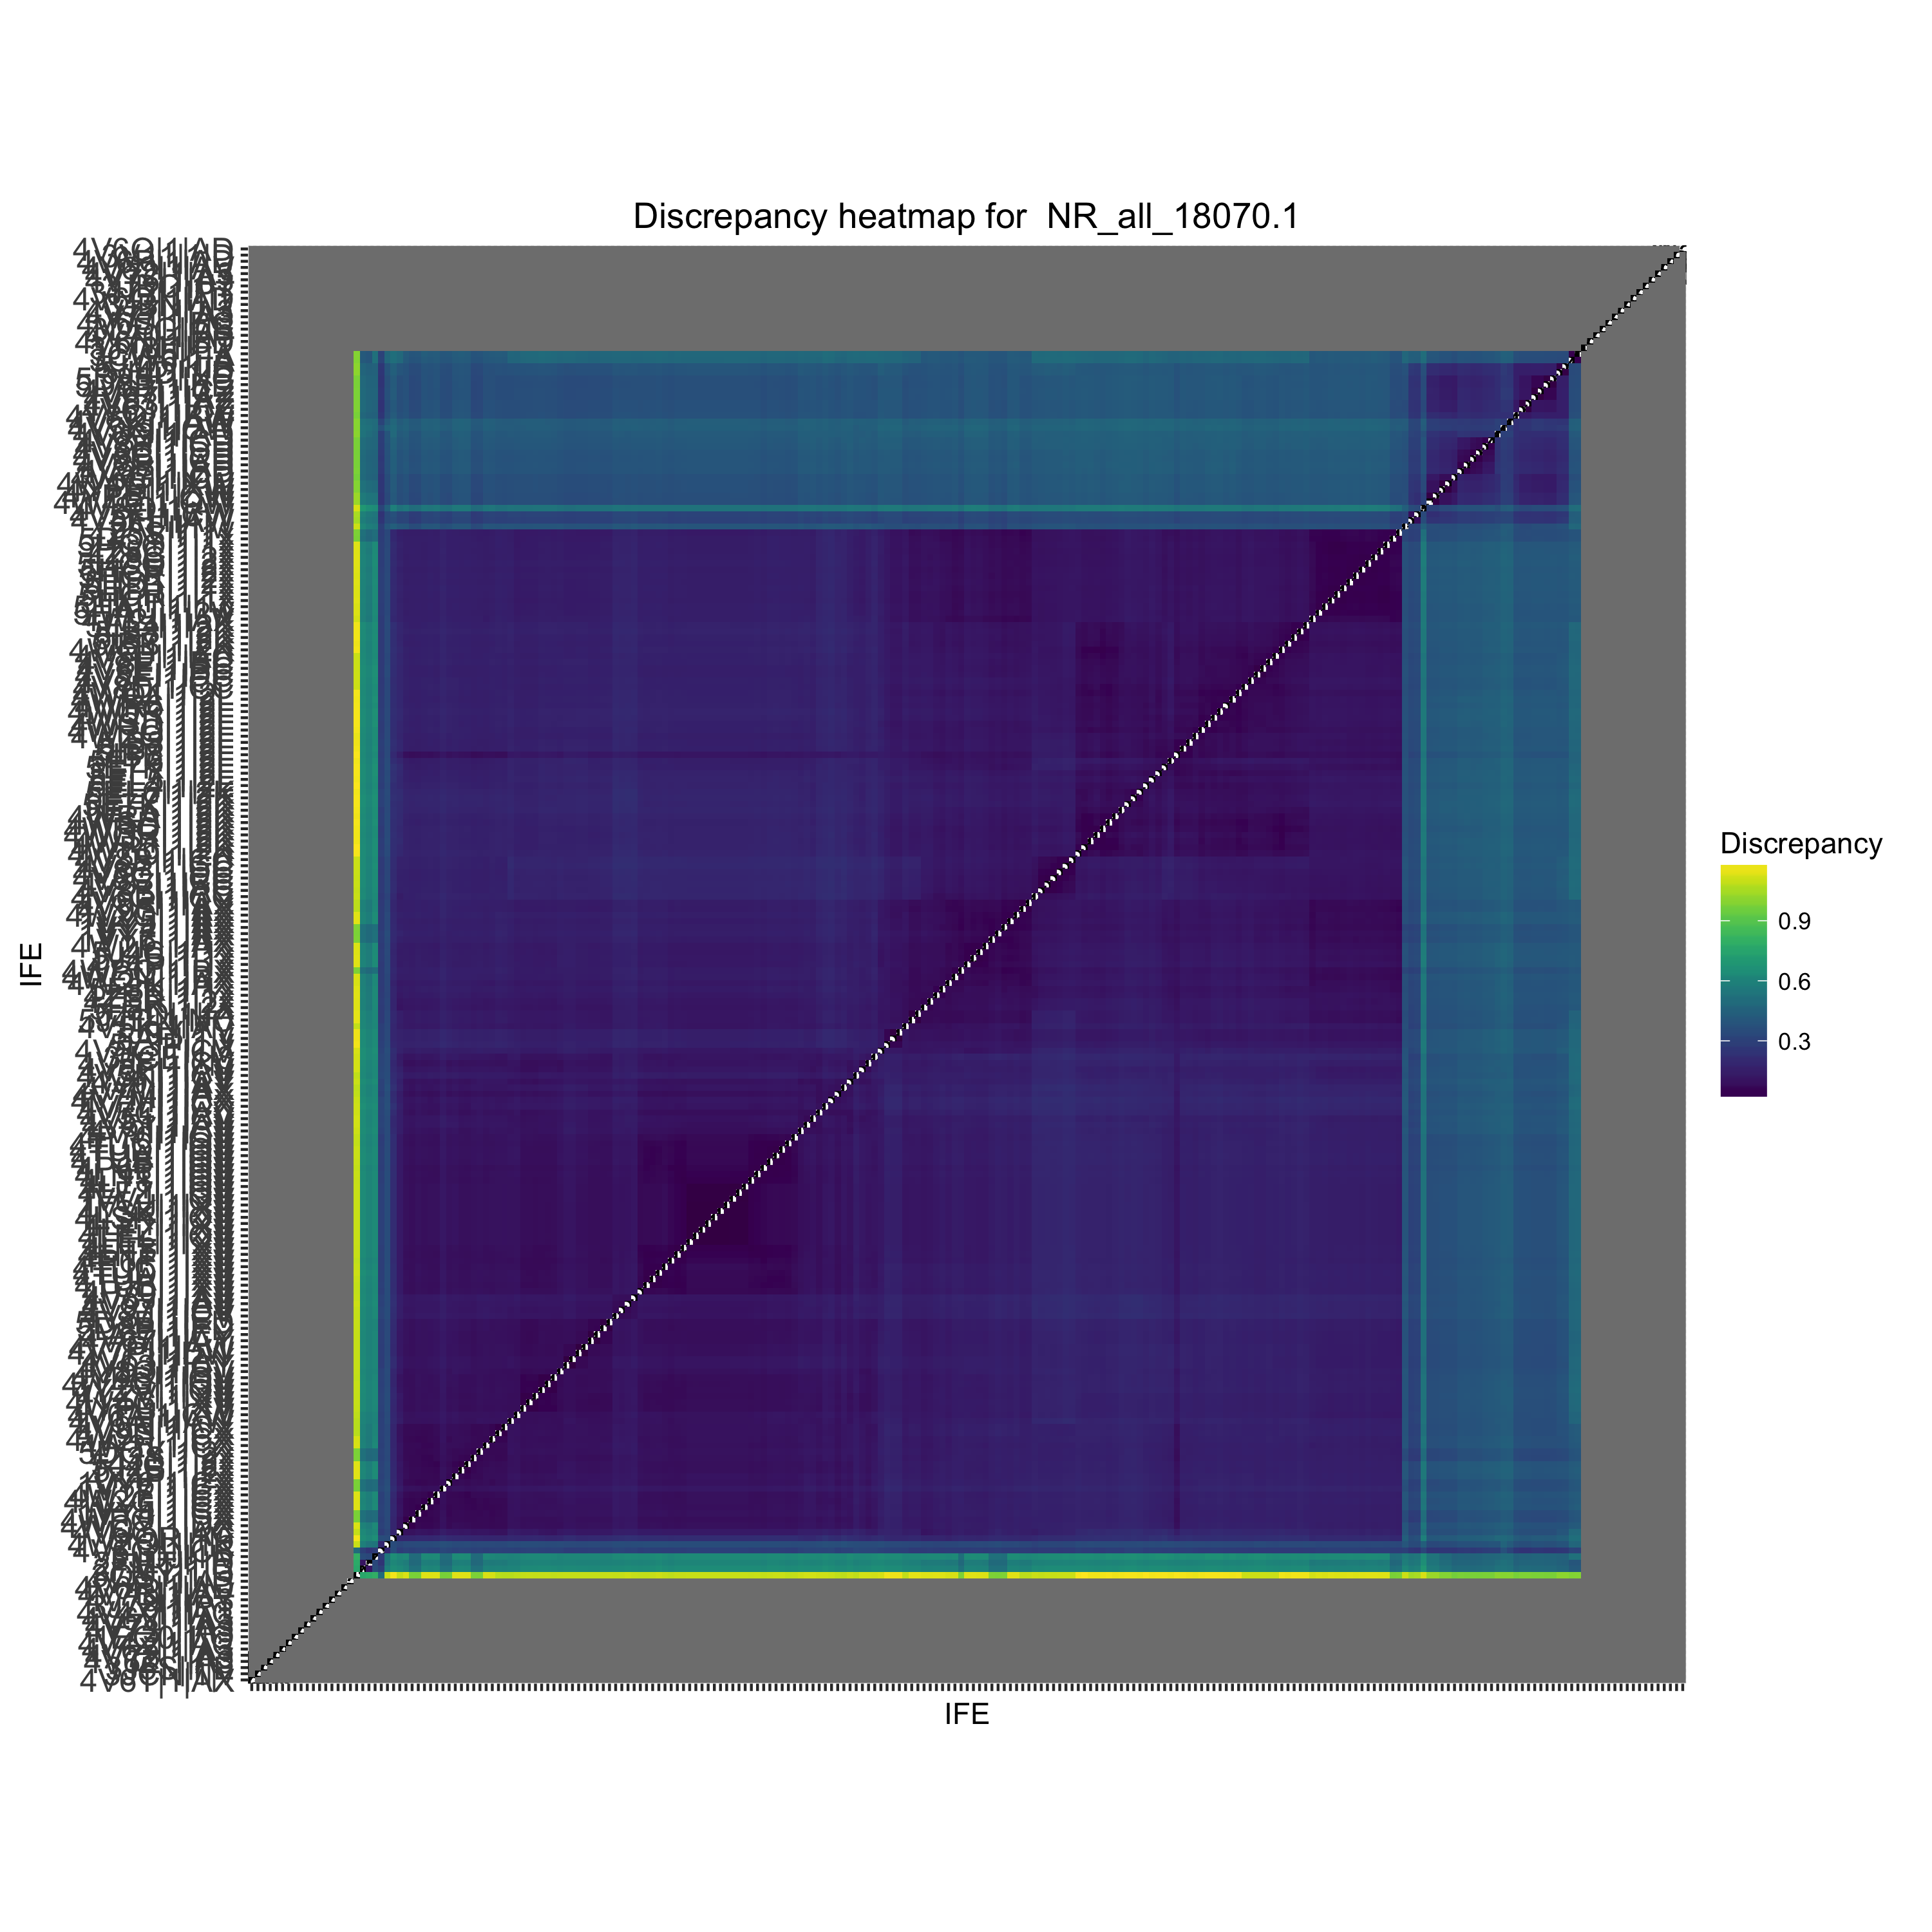
\includegraphics[width=\textwidth]{chapter-3/figs/nr-all-18070-1-disc}
  \caption{Figure summarizing the discrepancy heatmap for all IFE’s in
  NR\_all\_18070.1, a tRNA group with 233 members. }
  \label{fig:nr-all-18070.1-disc}
\end{figure}

The second NR\_all\_75770.1 is the second highest point on these plots. It is an
E. coli tRNA group with 170 members. There are a few IFE’s which are outliers
relative to the rest of the group. These chains appear to be fragments of the
larger tRNA. For example 1VY7 is a 5 nt fragment of the 76 nt tRNA.

We manually investigated the other groups with outliers and found that the
outliers are often placed into the same group because there is a structure that
we do not compute discrepancy for, such as a low resolution X-ray, that connects
the outliers to the rest of the group. For example, in previous version where we
did not compute discrepancy for NMR structures, an HIV hairpin would get joined
with a duplex of the same sequence because there was a NMR structure. All three
types of chains, the duplex, hairpin and NMR structure contained the same
sequence and thus were joined on the basis of sequence similarity. This was
resolved for NMR structures with the usage of discrepancy for them as well.
However, it remains an issue for low resolution X-ray and crystallography
experiments.

\section{Conclusions and future extensions}

Overall our grouping methodology successfully groups all chains into equivalence
classes. Our methodology is an improvement over the previous approach for
several reasons. First, it can work with mmCIF data by not only cluster the
largest chain in a file. Secondly, it computes and all discrepancies and
alignments to allow for future tuning of the parameters. Finally, our method
does not compute discrepancies for low resolution structures which will show
artificially high values.

There are several improvements that should be made. Notably, our method of
geometric similarity, discrepancy, is flawed for this task. It is too sensitive
to poor modeling in structures. Often the issue is the bases in nucleotides have
unusual orientations. If this was replaced with a different method that is less
sensitive to base orientation it may be possible  to compute all geometric
comparisons.

In addition, while evaluating the methodology it has been very useful to compute
a grouping using only sequences and then examine the changes when discrepancy is
applied. This could become part of the standard clustering procedure. For
example it may be useful to create a series of groupings built off each other.
The first a simple sequence only building, then adding species constraints, then
finally adding the discrepancy comparisons. This would make it easier to examine
our methodology as well as provide information about the linkages, if any
between groups. For example, there are likely many small groups that differ
structurally but have the same, or very similar sequences. Such groups may be
interesting for researchers interested the range of structures a single sequence
can form. A hierarchy of groupings could make this easier to determine.

Finally, small structures may well require a different set of rules for
comparison grouping. The work here was guided strongly by our experience with
ribosomes and tRNA molecules. These are much larger and show much clearer
differences than small synthetic molecules. It may be worthwhile to focus
exclusively on the small molecules to improve the methodology. For example, we
currently only use one chain when making geometric comparisons. This works well
with large molecules buy may not be accurate for small synthetic compounds. In
addition, it may be better to allow small chains to join through non-canonical
pairs as well as canonical cWW pairs. Doing so could allow us to build better
groups for the poly-A duplex or G-quadruplexes more accurately.

\chapter{SELECTION OF THE REPRESENTATIVE SETS FROM THE EQUIVALENCE CLASSES OF
RNA CONTAINING 3D STRUCTURES}

\section{Introduction and motivation}

The previous chapter discussed a method for organizing all RNA-containing 3D
structures in PDB into sets of equivalence classes. This procedure structures
the 3D dataset. However, for many use cases, simply organizing the data is
insufficient. In particular studies exploring the statistical properties of the
structural data set will be biased toward 3D structures that are highly
represented, as is currently the case with tRNA and ribosome structures. A
summary of is shown in Table~\ref{tab:mol-dist}.

\begin{table}
  \begin{tabulary}{\linewidth}{LRR}
    \toprule
    Molecule &
      Number of Integrated Functional Elements in the class &
      Percent of all RNA containing structures in PDB as of Sept 09, 2016 \\
    \midrule
    \TT{} LSU            & 282  & 4.0 \\
    \TT{} SSU            & 379  & 5.4 \\
    \TT{} 5S             & 282  & 4.0 \\
    \EC{} LSU            & 161  & 2.2 \\
    \EC{} SSU            & 157  & 2.2 \\
    \EC{} 5S             & 156  & 2.2 \\
    \HM{} LSU            & 69   & 0.9 \\
    \HM{} 5S             & 67   & 0.9 \\
    \DR{} LSU            & 42   & 0.5 \\
    \SC{} SSU            & 56   & 0.8 \\
    \SC{} LSU            & 63   & 0.9 \\
    Other Ribosomes      &      & \\
    Ribosomal Subtotal   & 1714 & 24.5 \\
    Remaining Structures & 5287 & 75.5 \\
    Total                & 7001 & 100 \\
    \bottomrule
  \end{tabulary}
  \caption{Proportion of solved structures that are from bacterial and yeast
    ribosomes. This table shows data from the 2.92 release of NR set at the
    'all' resolution, availabe at:
    \url{http://rna.bgsu.edu/rna3dhub/nrlist/release/2.92/all}. This dataset contains
    all structures available as of Sept 09, 2016. This table presents the
    fraction of the total structural database that comprises structures from all
    sources ribosomes. In total they make up 20\% of the solved crystal
  structures. LSU: Large Ribosomal Subunit, SSU: Small Ribosomal Subunit.}
  \label{tab:mol-dist}
\end{table}

As seen in the table, \EC{} and T. thermophilus ribosomes alone make up 20% of
the entire dataset and all ribosomal total NNN. For many statistical analyses of
RNA structure, it is desirable to identify one high quality representative
structure \cite{Leontis2012b}. For example, such a reduced redundancy dataset
set is desirable for constructing the RNA 3D Motif Atlas \cite{Petrov2013}. In
previous work a method to identify representative structures  from PDB format
files, called the non-redundant (NR) set was developed. We have updated the
method to take advantage of the new mmCIF data and fix limitations of the
previous method. These were posted on a weekly basis from February 5, 2011 to
December 5, 2014 on the BGSU RNA site and made available for searching on NDB
(\url{http://ndbserver.rutgers.edu/}).

\section{Requirements for representative set}

The set of representative structures has a variety of uses in structural
bioinformatics applications. Most notably it supports population and regular
updating of the RNA 3D Motif Atlas \cite{http://rna.bgsu.edu/rna3dhub/motifs}.
The RNA 3D Motif Atlas is a clustering of all high quality loops extracted from
all structures in the current Representative Set of structures. For this reason
it is desirable to avoid frequent changes in the representative structure due to
insignificant increments in the selection criteria. If we allow frequent
insignificant changes in the representative in structures selected for the
Representative set, these changes cause large changes in the RNA 3D Motif Atlas.
This makes the resource appear more unstable than it actually is and so we aim
to avoid changes due to minor improvements in structures. Thus the goals are of
the improvements described in this chapter are:

\begin{enumerate}
  \item The representative set should reflect observed variation in sequence,
    structure, and biological variation in the set of solved 3D structures

  \item The representative set should contain highest quality representative
    X-Ray structures from each Equivalence Class. NMR or Cyro-EM structures are
    chosen as representatives only when no X-ray structure is available.

  \item The representative set should only change upon the appearance of new,
    significantly better structures, using criteria explained in this chapter.
\end{enumerate}

The representative set is intended to display the observed structural, sequence,
and biological variation present in the current RNA-containing structural
dataset, avoiding duplication as much as possible. Each unique structural class
should be represented by one high quality structure, as the classes already take
into account the possibility of large structural variation, as explained in the
previous chapter. It is desirable to pick the highest quality structure
available from each equivalence class. A high quality structure is one that
models the experimental data as well or better than other available structures
and is as complete as possible.

\section{Methodology for selecting representative RNA 3D structures from
Equivalence classes}

This dissertation describes new methodology that represents significant
improvements over the previously developed methodologies of the BGSU RNA
resource. In the previous method, the Representative Structure from each
Equivalence Class was selected based solely upon the number of annotated base
pairs per nucleotide, discussed in detail in \cite{Leontis2012b}.

As the goal is to use only high quality structures the procedure uses X-ray
structures as the representative, if possible. Some structures, such as that of
the the mouse ribosome (3J7Q), have only been solved using cryo-electron
microscopy (``cryo-EM'') and in these cases, and only these cases,
representative selected for the equivalence set is necessarily a cryo-EM
structure. Only X-Ray structures are used when available because methods for
assessing the modeling quality of cryo-EM structures, comparable to RSR-Z scores
for X-ray crystallography are still under development and are not yet available
available (Berman, personal communication). Having object assessment data, like
RSR-Z scores available is essential for downstream applications such as
selecting reliable loops for inclusion in the Motif Atlas. As soon as
reliability data comparable to RSRZ scores are available for cryo-EM structures,
these structures will be treated on an equivalent footing as X-ray.

The procedure for each possible structure in:

\begin{enumerate}
  \item Select the structure with the most number of annotated basepairs per
    nucleotide.

  \item Find a structures with at least 1\% more bases and base pairs and select
    it as the current representative

  \item Repeat step 2 until there no structure has more base pairs and bases.
\end{enumerate}

This procedure has a few features that are worth discussing in detail. First, we
use the number of FR3D annotated cis Watson Crick/Watson Crick base pairs per
nucleotide (BP/NT) as the measure of structural quality because in our
experience a high quality model of the same RNA molecule contains more annotated
cWW base pairs than a poor model. This is a useful proxy and not a direct
measure of the modeling quality such as that provided by Real Space Refinement
(RSR) which is provided by PDB for all structures. RSR is measures how well a
structural model fits the underlying experimental data and is discussed in more
detail in the next chapter.

Secondly, this method is designed to select a structure based both on BP/NT but
also the number of nucleotides. Structures in the same class vary in the number
of resolved nucleotides. If we use only BP/NT then we may select a  smaller
structure that omits parts of the 3D structure that are less well modeled. We
prefer more complete representative structures over smaller structures and thus
include this second criterion.

Finally, the new method requires new representatives to show a significant
increase in both the number of nucleotides and the BP/NT. By doing so, we avoid
changing representatives upon insignificant changes in overall quality. Thus
stabilizing the Representative Set overtime. This 1\% increase is an empirically
determined cutoff that may be adjusted in the future. The new method of
representative selection described in this dissertation will be referred to
henceforth as the ``dual 1\% method''.

To describe the overall logic of the logic I have added a figure of the
pseudocode in Figure~\ref{fig:pseudocode-representatives}. This figure shows the
overall logic of this procedure, but does not correspond exactly to the
implementation.

\begin{figure}
  \caption{Pseudocode showing the overall logic of the selection for
  representative sets.}
  \label{fig:pseudocode-representatives}
\end{figure}

\section{Results of building the representative set}

I evaluated the Representative Set selected as described above by using the new
dual 1\% increase method, and compared results with the previous method and a
modification of the current method that changes the representative structure
based upon improvement of just one criterion. These classes used all available
structures from July 28, 2016. I will first discuss the differences between
structures selected by these methods and then move on to to examine the
stability of the methods.

\subsection{Selection of Structures for the Representative Set}

I evaluated the selection of representatives by examining the selection of
representatives from the equivalence classes built in the previous chapter. This
used all structures available as of July 25, 2016 (equivalent to release 2.86).
I examined classes for changes and determined where the new method selected
different representatives than the other methods. These changes were then
examined manually to assess the quality of the structures using the original as
well as additional criteria. There were 29 classes in the data set for which
different representatives were selected by the two methods. Shown in
Figure~\ref{fig:hm-lsu-rep} is a summary of the representative selection for the
three methods discussed here. The upper panel shows the previous method where we
can see the structure that is at the top of stack of very similar structures is
selected as the representative. This contrasts with our 1% increase method which
selects a example with more nucleotides and basepairs but a worse ratio of the
two. This selection is our desired result.

\begin{figure}
  \caption{Scatter plot of representative selection across three possible
    methodologies. Shown here is a summary of which IFE’s are selected as the
    representative for the 3 method discussed here. Each panel indicates a
    different method, in order from top to bottom, the previous method, a 1%
    increase method and the any increase method. Cyro-em structures are shown as
    circles, while X-ray are shown as triangles.  The representative IFE is
    colored in blue, while the other members of the set are colored red. The
    upper panel shows the previous method. It is difficult to see but the IFE
    selected as the representative is the IFE at the top of the stack of IFE’s
  in the upper right.}
  \label{fig:hm-lsu-rep}
\end{figure}

We then evaluated the selection of representative in context of the resolution
distribution. The ideal selection has the highest resolution of any structure in
the class. Show in Figure~\ref{fig:hm-rep-res-dist} is a summary. In it we can
see that all three methods select an IFE with resolution 2.4{\AA}. This is
consistent with our goals for the methods.

\begin{figure}
  \caption{Distribution of resolutions for IFE’s in NR\_all\_65634.1 with the
    resolution of the representative indicated. This histogram shows the
    resolution distribution of all IFE’s in the class. The red line indicates
  the resolution of the representative chosen by all 3 methods.}
  \label{fig:hm-rep-res-dist}
\end{figure}

We further evaluated the method described here by examining the selection of
representatives for the \EC{} Large and Small Subunits as well as the Thermus
thermophilus Large and Small Ribosomal Subunits, shown in
Figure~\ref{fig:ec-lsu-rep}, Figure~\ref{fig:ec-ssu-rep},
Figure~\ref{fig:tt-lsu-rep} and Figure~\ref{fig:tt-ssu-rep} respectively. As we
can see in these figures, only the \EC{} LSU T. thermophilus SSU differ in
selection of representatives.

\begin{figure}
  \caption{Scatter plot of the number of base pairs vs the number of nucleotides
    for selected \EC{} Large Subunits using the three methods discussed here.
    The representative selected is shown as a large blue dot, while all other
    members are shown as small red dots. The plot has been truncated to show
    only the structures with at least 2840 nucleotides and 500 basepairs for
  clarity.}
  \label{fig:ec-lsu-rep}
\end{figure}

\begin{figure}
  \caption{Scatter plot of the number of base pairs vs the number of nucleotides
    for selected \EC{} Small Subunits using the three methods discussed here.
    The representative selected is shown as a large blue dot, while all other
    members are shown as small red dots. The plot has been truncated to show
    only the structures with at least 1400 nucleotides and 300 basepairs for
  clarity.}
  \label{fig:ec-ssu-rep}
\end{figure}

\begin{figure}
  \caption{Scatter plot of the number of base pairs vs the number of nucleotides
    for selected T. thermophilus Large Subunits using the three methods
    discussed here. The representative selected is shown as a large blue dot,
    while all other members are shown as small red dots. The plot has been
    truncated to show only the structures with at least 2725 nucleotides and 500
  basepairs for clarity.}
  \label{fig:tt-lsu-rep}
\end{figure}

\begin{figure}
  \caption{Scatter plot of the number of base pairs vs the number of nucleotides
    for selected T. thermophilus Small Subunits using the three methods
    discussed here. The representative selected is shown as a large blue dot,
    while all other members are shown as small red dots. The plot has been
    truncated to show only the structures with at least 1490 nucleotides and 200
  basepairs for clarity.}
  \label{fig:tt-ssu-rep}
\end{figure}

\subsubsection{Evaluating representative selection on the basis of resolution}

Another useful criteria for evaluation our representative selection is to
examine if our method selects the structure with lowest resolution. Generally,
higher resolution structures are better than lower resolution structures. To
explore this I computed the difference between the selected representative for
all groups and the structure in the group with the smallest resolution. A
summary of this data is shown in Table~\ref{tab:res-diff-summary}.

\begin{table}
  \begin{tabulary}{\linewidth}{LRRR}
    \toprule
    Method &  Representatives with lowest resolution &  Representatives with
    resolution within 1{\AA}  & Representatives with resolution > 1{\AA} \\
    \midrule
    Previous          & 1506 (93\%) & 86 (5.3\%) & 14 (0.8\%) \\
    Dual Increase     & 1494 (93\%) & 97 (6.0\%) & 15 (0.9\%) \\
    Dual 1\% Increase & 1506 (93\%) & 88 (5.4\%) & 12 (0.7\%) \\
    \bottomrule
  \end{tabulary}
  \caption{A summary of the differences between the resolution of the
  representatives as compared to the member of the group with the lowest
  resolution.}
  \label{tab:res-diff-summary}
\end{table}

From this we can see that nearly all groups use a structure with the lowest
resolution, as we desired. However, roughly 5\% of all groups have a
representative with resolution with 1{\AA} of the minimum. This leaves a very small
percent, less than 1\%, of all groups that use a representative with resolution
greater than 1{\AA} from the minimum. Shown in Figure~\ref{fig:res-diff-histogram}
is a histogram that displays the differences for all groups where the difference
is greater than 0{\AA}.

\begin{figure}
  \caption{Histogram of the differences between the resolution of the selected
    representative and the minimum resolution within the group for all 3
    methods. This histogram does not show the groups where the representative
    resolution is the same as the minimum resolution.  The red vertical line
    indicates the cutoff of 1{\AA}. The numbers to the left of the red box indicate
    the total number of groups with resolution difference less than 1{\AA}, while
    the number to the right indicates the number of groups with resolution
  difference greater than 1{\AA}.}
  \label{fig:res-diff-histogram}
\end{figure}

From this figure we can see two things. First, all methods are very similar in
terms of the number of groups that select representatives with unusually high
resolution. Secondly, several groups have very large differences between the
selected representative and the minimum resolution. For example one group has a
difference of 14\AA. Examining this data shows that there are 19 groups with
resolution differences. Shown in Table~\ref{rep-res-diff-details} are the
summary of those groups.

\begin{table}
  \begin{tabular}{llrrr}
    \toprule
    Group &  Minimum Resolution ({\AA}) &  Previous &  Dual Increase &  Dual 1\% Increase \\
    \midrule
    NR\_all\_00304.1 &  9.0  & \ife{3J0D}{1}{A} (11.1{\AA}) [2.1{\AA}]  &
                               \ife{3J0D}{1}{A} (11.1{\AA}) [2.1{\AA}]  &
                               \ife{3J0D}{1}{A} (11.1{\AA}) [2.1{\AA}]  \\
    NR\_all\_13601.2 &  5.0  & \ife{4KZZ}{1}{j} (7.03{\AA}) [2.03{\AA}] &
                               \ife{4KZZ}{1}{j$ (7.03{\AA}) [2.03{\AA}] \\
    NR\_all\_14586.1 &  3.5  & \ifePair{4V6X}{1}{A5}{4V6X}{1}{A8} (5{\AA}) [1.5{\AA}] &
                               \ifePair{4V6X}{1}{A5}{4V6X}{1}{A8} (5{\AA}) [1.5{\AA}] \\
    NR\_all\_16577.1 &  6.9  & \ife{3J0O}{1}{V} (9{\AA}) [2.1{\AA}] &
                               \ife{3J0O}{1}{V} (9{\AA}) [2.1{\AA}] &
                               \ife{3J0O}{1}{V} (9{\AA}) [2.1{\AA}] \\
    NR\_all\_18070.1 &  2.4  & \ife{4TUD}{1}{QV} (3.6{\AA}) [1.2{\AA}] \\
    NR\_all\_33599.2 &  2.6  & \ife{4V5M}{1}{AV} (7.8{\AA}) [5.2{\AA}] \\
    NR\_all\_33884.1 &  3.45 & \ife{4KZY}{1}{i} (7.01{\AA}) [3.56{\AA}] &
                               \ife{4KZY}{1}{i} (7.01{\AA}) [3.56{\AA}] \\
    NR\_all\_37074.2 &  2.1  & \ife{4V6Z}{1}{BB} (12{\AA}) [9.9{\AA}]   &
                               \ife{5J88}{1}{DB} (3.32{\AA}) [1.22{\AA}] \\
    NR\_all\_39327.1 &  3.8  & \ife{4V6M}{1}{AV} (7.1{\AA}) [3.3{\AA}]   &     
                               \ife{4V6M}{1}{AV} (7.1{\AA}) [3.3{\AA}] &
                               \ife{4V6M}{1}{AV} (7.1{\AA}) [3.3{\AA}] \\
    NR\_all\_39428.1 &  2.6  & \ife{4V8U}{1}{CV} (3.7{\AA}) [1.1{\AA}] &
                               \ife{4V8U}{1}{CV} (3.7{\AA}) [1.1{\AA}] &
                               \ife{4V8U}{1}{CV} (3.7{\AA}) [1.1{\AA}] \\
    NR\_all\_44399.2 &  2.96 & \ife{4V70}{1}{A1} (17{\AA}) [14.04{\AA}] \\
    NR\_all\_48374.2 &  2.1  & \ife{1C04}{1}{F} (5{\AA}) [2.9{\AA}] &
                               \ife{1C04}{1}{F} (5{\AA}) [2.9{\AA}] &
                               \ife{1C04}{1}{F} (5{\AA}) [2.9{\AA}] \\
    NR\_all\_55323.1 &  3.71 & \ife{4V68}{1}{AY} (6.4{\AA}) [2.69{\AA}] \\
    NR\_all\_59913.2 &  2.1  & \ife{4V4Q}{1}{CA} (3.46{\AA}) [1.36{\AA}] &
                               \ife{4V4Q}{1}{CA} (3.46{\AA}) [1.36{\AA}] &
                               \ife{4V4Q}{1}{CA} (3.46{\AA}) [1.36{\AA}] \\
    NR\_all\_62116.2 &  2.1  & \ife{4V54}{1}{DB} (3.3{\AA}) [1.2{\AA}] \\
    NR\_all\_68375.1 &  8.3  & \ife{3IZ4}{1}{A} (13.6{\AA}) [5.3{\AA}] &
                               \ife{3IZ4}{1}{A} (13.6{\AA}) [5.3{\AA}] &
                               \ife{3IZ4}{1}{A} (13.6{\AA}) [5.3{\AA}] \\
    NR\_all\_87281.1 &  3.9  & \ife{3J3V}{1}{B} (13.3{\AA}) [9.4{\AA}] \\
    NR\_all\_95973.1 &  3.8  & \ife{4D61}{1}{j} (9{\AA}) [5.2{\AA}] &
                               \ife{4D61}{1}{j} (9{\AA}) [5.2{\AA}] &
                               \ife{4D61}{1}{j} (9{\AA}) [5.2{\AA}] \\
    NR\_all\_97012.1 &  2.0  & \ife{4V49}{1}{AW} (8.7{\AA}) [6.7{\AA}] &
                               \ife{4V49}{1}{AW} (8.7{\AA}) [6.7{\AA}] &
                               \ife{4V49}{1}{AW} (8.7{\AA}) [6.7{\AA}] \\
    \bottomrule
  \end{tabular}
  \caption{}
  \label{tab:rep-res-diff-details}
\end{table}

The new method will not select a cryo-EM structure if an X-ray structure is
available, however, new cryo-EM structure are being solved with increasingly
higher accuracy, rapidly approaching the quality of X-ray structures. This is a
potential reason for the differences found in Table~\ref{tab-res-diff-details}.
I examined this by determining the difference between the resolution of the
representative structure and the minimal resolution in that group for all
groups, using only X-ray structures and repeating the analysis. Shown in
Figure~\ref{fig:xray-only-diff} is this figure.

\begin{figure}
  \caption{}
  \label{fig:xray-only-diff}
\end{figure}

In this figure we can see that there are very few groups have resolution
difference greater than 1\AA{} for all methods. As with the previous analysis, all
methods perform similarly in terms of the number of groups with large
differences. However, the Dual 1\% method does show a smaller resolution
difference. Shown in Table~\ref{tab:xray-only-outliers} are the groups with large
difference between the representative resolution and minimum resolution.

\begin{table}
  \begin{tabular}{llrrr}
    \toprule
    Group &  Minimum Resolution ({\AA}) &  Previous &  Dual Increase  & Dual 1\% Increase \\
    \midrule
    \bottomrule
  \end{tabular}
  \caption{}
  \label{tab:xray-only-outliers}
\end{table}

From this table we can see that the Dual 1\% increase has the fewest differences.
In addition, the times it does have issues are the same as the previous method,
indicating this method is not making new mistakes.

Overall, I note that the new method, Dual 1\% Increase, almost always, greater
than 90\% of the time, selects a representative that has a resolution close to
the best nominal resolution in the group. This is desirable because higher
resolution generally means a better structure. However, there are very few cases
w’here this does not occur. The new method performs better than the previous
version as there are fewer of these cases and the difference in resolution is
smaller. Many of these cases appear to be due to the group containing both
cryo-em and x-ray structures. The new method, by construction, will always
prefer X-ray structures, even when the nominally higher resolution is a cryo-EM
structure.

\subsubsection{Independent measures of representative selection}

PDB provides quality reports for all structures \cite{Gore2012}. These quality
reports use a variety of metrics that were suggested by the X-ray validation
task force \cite{Gore2012}. Here I evaluate our selection on the basis of data
from these quality reports. Shown in Figure~\ref{fig:ec-lsu-report} is the
quality report for the representative selected by the dual 1\% increase method
as compared to that of the previous method. From this figure we can see that the
dual 1\% increase method selects structures with fewer RSRZ outliers and similar
RNA backbone scores, however, all other metrics are worse.

\begin{figure}
  \caption{Screenshots of the summaries of quality reports for 4V54 (left), the
    representative selected by the Dual 1\% increase method as compared to the
    report for 5J91 (right), the representative selected by the previous
  method.}
  \label{fig:ec-lsu-report}
\end{figure}

The same data is shown for the Thermus thermophilus large subunit group in
Figure~\ref{tt-lsu-report}. In this case we see that both structures have very
similar metrics overall. The previous method does select a structure, 5HCQ, with
fewer RSRZ outliers.

\begin{figure}
  \caption{Screenshots of the summaries of quality reports for 5FDU (left), the
    representative selected by the dual 1% increase method as compared to the
    report for 5HCQ (right), the representative selected by the previous
  method.}
  \label{fig:tt-lsu-report}
\end{figure}

These figures indicates that while the dual 1\% increase method does not use the
quality metrics, it does select a good structure.

\subsection{Stability of the Representative Set}

In order to asses the stability of our method we computed the representatives
for a set of 91 weekly releases from 2.0 to 2.90 covering releases from December
5, 2014 to August 26, 2016 using the three methods. We then plotted the number
of changes in the representatives for all equivalence class that are common to
all releases. We expect that the any increase method will be the most unstable,
with the previous and current method being comparable. Our goal is the current
1\% increase method will be more stable. The summary is shown in
Figure~\ref{fig:rep-changes}. This plot summarizes the total number of changes
for 1449 classes that exist in all 91 releases. We can see that all three
methods are comparable in stability, as they all end near 25 total changes. In
general both the 1\% increase and the previous method are more stable, show fewer
changes, than the any increase method. For most of the plot our current method
shows as many or fewer changes than the previous, indicating it is slightly more
stable.

\begin{figure}
  \caption{A cumulative distribution of the total number of changes for all
    three methods. This plot is a cumulative sum of the total number changes for
    all classes at the ``all'' resolution cutoff which exist in all of the 90
  releases used in the analysis.}
  \label{fig:rep-changes}
\end{figure}

We examined the number of total number of changes for each class in the dataset.
As shown in Table~\ref{tab:rep-changes-count} most classes that exist in all the
releases show no changes. Of those that show changes the majority change only 1
time.

\begin{table}
  \begin{tabular}{lrrrrr}
    \toprule
                        & \multicolumn{5}{c}{Number of Changes} \\
    % \cmidrule{r}{2-6}
    Method              & 0    & 1  &  2 &  3 &  4 \\
    \midrule
    Previous Method     & 1528 & 19 &  0 &  2 &  0 \\
    Any Increase Method & 1530 & 17 &  0 &  3 &  0 \\
    1\% Increase Method & 1529 & 16 &  0 &  2 &  1 \\
    \bottomrule
  \end{tabular}
  \caption{Number of changes for classes that exist from 2.0 to 2.90. This table
    summarize the number of classes that show 0, 1, 2, 3, or 4 changes amongst
  the classes that exist in all releases. }
  \label{tab:rep-changes-count}
\end{table}

To see how often classes with more than 1 change alters the representative we
plotted all classes that show more than one change across these releases as seen
in Figure~\ref{fig:multi-change}. We see that there are only 3 classes that show
this behavior: 80570, a 2 nucleotide synthetic RNA, 83717 the \EC{} LSU, and
97519 the T. t LSU. From this we can see that all methods are generally stable
for many releases followed by a few very quick changes. This is more
desirable over a method which changes very frequently. One class, 80570
shown in red, the representative is changed every time a new structure is
added by all methods. This class has few members, 8 in 2.90, and a very
few nucleotides, leading to minor changes in resolution changing the
selected representative. Shown in Figure CONSTANT CHANGE are the
structures of the representative in 2.0 and 2.90. From this we can see
that the structures are highly similar

\begin{figure}
  \caption{This figure shows the rate of changes in for each class that changes
    more than once between 2.0 and 2.90. Each colored line represents a class,
    and each mark indicates when members are added to the class. The three sets
  panels indicate the three different methods tested here.}
  \label{fig:multi-change}
\end{figure}

\section{Conclusions and future work}

In summary, we have developed a method to select a representative structure from
our equivalence classes. This method reliably selects a good structure from the
set of structures. It is also stable and will not change due to small
improvements in the structure.

One possible improvement is to use the quality metrics provided by PDB, such as
real space refinement (RSR) and the RSR Z-score (RSRZ) in the selection of the
representative structure. These are measures of how well a modeled structure
fits the underlying data from the experiment. This data and its utility will be
discussed in detail in the following chapter. Usage of this data will allow us
to detect if a structure is well modeled. This could be used in place of our
base pairs per nucleotides metric to select structures. The downside is that not
all structures have RSRZ data. Notably, cyro-em structures do not yet have such
a metric. The community is working on such metrics however.

\chapter{SELECTION OF LOOPS FOR CLUSTERING IN THE RNA 3D MOTIF ATLAS FROM THE
REPRESENTATIVE SET OF STRUCTURES}

In this chapter I will discuss the changes I have made to the way the BGSU RNA
pipeline selects loops for building the RNA 3D Motif Atlas
(\url{http://rna.bgsu.edu/rna3dhub/motifs}). The goal of our Motif Atlas is to
maintain a high quality, up-to-date clustering of representative RNA 3D Motifs
(hairpin, internal, and multi helix junction loops) from the 3D structure
database, on an ongoing basis. An important step in of building the Motif Atlas
is the selection of loops. The original process of selecting loops was
implemented by Dr. Anton Petrov in previous work \cite{Petrov2012}. Overall, the
procedure worked as follows: First, all loops from all representative from the
all 4.0{\AA} equivalence classes are extracted. This representative was always
the longest chain in a PDB file. Then each loop was examined for the presence of
possible structural flaws, which serve as criteria for removal. In the previous
version the representative was only the longest chain in each file. The loop
exclusion criteria criteria included:

\begin{enumerate}
  \item Presence of chain breaks in the loop. Chain breaks occur when the
    phosphate backbone of the molecule is not continuous. This occurs due to
    modeling issues, or a lack of electron density in the affected region.

  \item Presence of a self-complementary sequence in a nominally unpaired
    internal loop. These loops are often a poorly modeled helixes that appear as
    loops in our method.

  \item Presence of incomplete nucleotides. Incomplete nucleotides occur when
    only part of a nucleotide is modeled. In some structures only electron
    density for the backbone is observed, leading to models that lack the base
    in some nucleotide positions
\end{enumerate}

Examples of these structural issues are shown in
Figure~\ref{fig:loops-with-issues}. These criteria all examine the structure of
the loops for signs of data incompleteness or modeling flaws. If any loop shows
one these problems it is rejected from clustering.

\begin{figure}
  \caption{Examples of loops with structural problems.}
  \label{fig:loops-with-issues}
\end{figure}

In addition to these structural issues, the previous also rejects loops that
have been incorrectly extracted. This occurs when a single loop contains too
many chains. For example, an internal loop composed of 3 or more chains would be
rejected. An example of such a loop IL\_3OL6\_001 is shown in
Figure~\ref{fig:too-many-chains}.

\begin{figure}
  % \includegraphics{chapter-5/figs/IL_3OL6_001}
  \caption{3D structure of an internal loop with too many chains. This loop
    IL\_3OL6\_001 is rejected by our loop quality procedures because it contains
    too many chains, 3 in this case, loops for a valid internal loop.}
  \label{fig:too-many-chains}
\end{figure}

Finally, the previous method rejects loops that contain modifications. This is
because our current FR3D cannot process modified bases \cite{Sarver2008a}. We are
currently working on removing this limitation. An example of such a loop is
shown in Figure~\ref{fig:modified-loop}.

\begin{figure}
  % \includegraphics{chapter-5/figs/IL\_4YBB\_320}
  \caption{3D structure of, IL\_4YBB\_320, an internal loop with modified bases.
  This internal loop is currently rejected with our loop quality steps.}
  \label{fig:modified-loop}
\end{figure}

My changes to the loop selection process are in three areas. First, I improved
the selection criteria to take advantage of additional information available in
mmCIF data. For example, mmCIF data includes information on atom occupancy.
Secondly, I altered the logic to include the capability to exclude loops from
cryo-EM data for some versions of the Motif Atlas. Finally, I have used a
measure of modeling quality, Real Space R Z-Score (RSRZ), to exclude loops
outside certain statistical limits. I tested different thresholds for RSR-Z and
their effects. I will discuss each of these changes in turn.

\section{Modifications to Previous Loop Selection Methodology}

The first change was to take advantage of new information in mmCIF data. This
change affected two of the criteria, how the presence of chain breaks and
the presence of incomplete nucleotides are detected.

Previously, chain breaks were detected by measuring the distance between the
phosphate atom of one nucleotide and the O3` of the preceding nucleotide. This
distance should be less than 2{\AA} \cite{Petrov2012} when a covalent bond is
present. This approach requires computing bond distances between all successive
pairs of nucleotides and comparison to a free parameter that requires selection.
The new format, mmCIF, provides a mapping between the observed sequence and the
experimental sequence. In this mapping, chain breaks are detected as nucleotide
positions in the experimental sequence that are not mapped to observed
sequences, ie the nucleotides for which no 3D coordinates are provided. By
using the experimental sequence mapping we no longer need to measure distances
in the structure to make this decision.

The second affected criterion, presence of incomplete nucleotides has been
extended to include atoms with zero occupancy. The previous procedure rejected
any loop that contained any nucleotide that lacked all the required atoms. This
occurs when an author chooses not to model a nucleotide because of missing  or
incomplete electron density data. However, some authors will model nucleotides
for which there is incomplete data and then mark one or more of the atoms of
that nucleotide as having zero occupancy (CITE). My new procedure will now
detect these cases by checking the occupancy data for each atom of each
nucleotide of the loop. In the case that the occupancy for one or more atoms in
a loop is zero, the entire loop is excluded from clustering. The new logic is
more rigorous and removes more loops than the previous method.
Table~\ref{tab:loop-quality-changes} compares the effects the new selection
criteria to the last Motif Atlas with the Petrov method in December 2014.

Finally, when beginning to work with mmCIF data, I found a bug in our loop
extraction procedure that inadvertently extracted loops formed by molecules
related by symmetry operators in the crystal structures. To fix this bug has
added a new criteria to ensure that we do not extract loops formed by
nucleotides generated by more than one symmetry operator.  In other words
we do not extract loops created by crystal contacts.

These changes alter the loop selection logic. Shown in
Table~\ref{tab:loop-quality-changes} is a comparison between the new and
previous method. I took all accepted loops from the Motif Atlas Release 1.18,
which are from representative structures from the 2.85 Representative release
and determined their status using the new logic. The counts are compred in
Table~\ref{tab:loop-quality-changes}, which shows that that the majority of
loops will have the same classifications, but a small percent do change.

\begin{table}
  \begin{tabulary}{\linewidth}{LLRRRR}
    \toprule
    Loop Type &
      Previous Accepted Loops (1.85) &
      Currently Accepted Loops (2.86) &
      Missing Nucleotides &
      Modified with Nucleotides &
      Incomplete Nucleotides \\
    \midrule
    Hairpin Loops  & 736 & 708 & 15 & 6 & 7 \\
    Internal Loops & 933 & 914 & 4  & 6 & 9 \\
    \bottomrule
  \end{tabulary}
  \caption{A table showing the numbers of loops affected by the changes to the
    selection procedure to address incomplete or flawed loop data or models. The
    number in parenthesis in the header indicates the representative release
    for that column.}
  \label{tab:loop-quality-changes}
\end{table}

\section{Exclusion of loops from cryo-Electron Microscopy}

The next change to loop selection, exclusion of loops from cryo-EM structures,
is a simple addition with a large effect. Currently, X-Ray structure
determination is the ``gold standard'' of structural methods for large
biomolecules (CITE). There is a great deal of exciting work using cryo-electron
microscopy (cryo-em) to determine structures of large biomolecules that form
multiple conformational states \cite{Amunts2014, Quade2015, Schureck2016}.
However, this technique is under rapid development and still lacks defined
criteria for assessing structural quality on a par with the standards that are
already well-established for X-ray structures \cite{Henderson2012}. We plan to
carry out the loop extraction procedure in two ways, with and without loops
loops that come from structures solved by \cyem, until defined criteria re
established and we can integrate cryo-EM loops in the ``gold standard'' Motif
Atlas release. Comparison of the two releases will allow monitoring of new
motif geometries that are only found in \cyem structures.

Rejecting loops from \cyem structures has a large effect on the number of loops
available for clustering. As a test of this I extracted all loops from the
representative set, representative release 2.86, described in the previous
chapter and then counted the number of valid loops from each source.  Shown in
Table~\ref{tab:source-counts} is a summary of counts of valid internal loops.

\begin{table}
  \begin{tabulary}{\linewidth}{LLRRRRRR}
    \toprule
                             &                 & \multicolumn{3}{c}{Number of Valid Internal Loops} & \multicolumn{3}{c}{Number of Valid Hairpin Loops} \\
    Representative           & Number of IFE's & X-ray & \cyem & Total & X-ray & \cyem & Total \\
    \midrule
    1.18 (December 05, 2014) & 858  & 1653 (69\%) & 757 (31\%)  & 2410 (100\%) & & & \\
    2.85 (July 28, 2016)     & 1232 & 1945 (50\%) & 1951 (50\%) & 3896 (100\%) & & & \\
    \bottomrule
  \end{tabulary}
  \caption{Counts of the number of valid loops from X-ray vs \cyem{} structures.
  This table highlights the large growth of \cyem{} loops.}
  \label{tab:source-counts}
\end{table}

The comparison in Table~\ref{tab:source-counts} shows that there is a much
larger growth over the past \TILDE 20 months in the number of loops present in
from \cyem structures.

When not using cryo-EM loops, we reduce the number of internal loops available
for clustering by half for release 2.85 by half bringing the number of selected
internal loops, from 3896 to 1945. This total is fewer than number used in the
previous motif release, 2410. This change has a large effect on the selection of
loops and thus the final clustering of motifs.

\section{Usage of Real Space R data for loop selection}

The final change to the loop selection procedure implemented is to use modeling
quality data from PDB as an additional criterion measuring how well 3D models
determined by X-ray crystallography reflect the underlying electron density. The
Petrov \etal selection procedure successfully detected structural
deficiencies of the loops but did not consider modeling issues
\cite{Petrov2012}. The new changes apply the modeling criteria the recently made
available by PDB for each X-ray structure, the Real Space Refinement (RSR)
statistic and the RSR Z-Score (RSRZ) statistical score. RSR directly measures
how well the 3D model fits the underlying experimental electron density. I begin
with a discussion of the new RSRZ scores and discuss the modifications to our
quality criteria and their consequences on the numbers of structures retained.

\subsection{Description of Real Space Refinement and the associated Z-Score}

Real Space Refinement (RSR) is a measure of how well the atomic resolution 3D
model present in a PDB file fits the observed, underlying electron density
obtained by X-ray diffraction. This was originally described by Jones \etal in
the development of Uppsala validation server \cite{Kleywegt2004a}. RSR is
calculated using equation:

\begin{equation}
  RSR = \frac{\sum \mid \rho_{obs} - \rho_{calc} \mid}
             {\sum \mid \rho_{obs} + \rho_{calc} \mid}
\end{equation}

where $\rho$ is electron density. In words this equation computes the normalized
difference between the observed electron density and modeled electron density. I
explored the distribution of the RSR values for all nucleotides in loops. This
is shown in Figure~\ref{fig:rsr-nt-distribution}.

\begin{figure}[ht]
  \caption{Histograms of the distribution of RSR values for nucleotides in
    loops. Each panel represents a different residue. The loop used are all
    accepted loops from Representative release 2.85. The blue bars indicate the mean
  of each distribution.}
  \label{fig:rsr-nt-distribution}
\end{figure}

This figure shows that MORE.

There are several issues with RSR however \cite{Tickle2012}. To deal with these
issues, the corresponding Z-score, statistical measure, RSRZ, has been proposed
for general use \cite{Gore2012}. The Real Space Z-Score (RSRZ) is a normalized
version of RSR calculated by PDB. This data is calculated for each structure on
a residue level. The data is produced by computing RSR Z-Scores for each type of
residue present in the structure and comparing to like residues in all other
comparable structures of similar resolution, ie A's are compared to other A's,
while C's are compared to other C's \cite{Gore2012, Kleywegt2004a}. PDB provides
this statistic as part of their validation reports and the data is imported as
part of our weekly update pipeline. This data is available on their FTP site,
the URLs depend upon the structure, for example the data for 1FJG is available
at: \url{http://ftp.wwpdb.org/pub/pdb/validation\_reports/fj/1fjg/}. In this way
the quality of each structure is compared to other structures of comparable
resolution, as well as to all other X-ray structures in PDB that contain RNA.

\subsection{Determining how to use RSRZ to reject loops}

We begin by examining the distribution of RSRZ data for each type of loop in the
representative set of 3D structures selected as described in the previous
chapter, which corresponds to the 2.85 representative structure release
available at (\url{http://rna.bgsu.edu/rna3dhub/nrlist/release/2.85}). The
distribution of such data is shown in Figure~\ref{fig:rsrz-distribution}. In
this figure we can see that loops nucleotides have a median value near 0,
indicating a good fit to observed density. We can also see a long tail in the
RSRZ distribution that indicates a large range in the quality of modeling. PDB
assigns an RSRZ value of 2 to indicate a large outlier. This is shown on the
graphs as a red bar.

\begin{figure}
  \caption{Distribution of RSRZ values for nucleotides in all accepted loops.
    The nucleotides are only from loops that pass all structural criteria.}
  \label{fig:rsrz-distrubution}
\end{figure}

From this distribution we can see that median value is less than 0. This
indicates that loops in bases from our representative structures are better
modeled than the average nucleotide. This supports the conclusions of the
previous chapter that appropriate criteria are used to select the representative
structure. However, there is a long tail of nucleotides with very high values.
Loops with containing poorly modeled nucleotides that should be excluded from
clustering and inclusion in the 3D Motif Atlas. I used RSRZ values to create two
criteria. The first is that all bases in a loop must be well modeled, that is
all nucleotides in the loop should have a low RSRZ value. I use this cutoff
because we want to ensure that a loop is not an ``appealing fiction'' where all
bases in it are poorly modeled. We do not consider if the bases are interacting
in this criterion because some loops do not contain interactions. Secondly, is
that all nucleotides that make interactions with other bases within the loop
must have a low RSRZ value as well. This criterion is used because we expect
that loops interacting within a loop will have a lower RSRZ value by virtue of
being ``fixed in place'' in the crystal.

\subsection{Detecting fictional loops}

The first criterion is that all bases in a loop should be sufficiently well
modeled. A well modeled base has a low RSRZ value, thus a poorly modeled loop is
one where all modeled bases in the loop have a high RSRZ value. I will refer to
these loops as ``poorly modeled’. We are interested in explore the effect of
various RSRZ cutoffs on motif clustering so we will use a range of values. We
have been advised by PDB to implemented an RSRZ threshold of 2 to identify loops
that are poorly modeled. I tested cutoffs of 1, 1.5 and 2.5 to explore the
effect of various cutoffs on motif clustering. I applied this criterion, all
nucleotides in the loop must have an RSRZ less than the cutoff, to all valid
loops in the dataset. A summary of the number of loops sorted by this criterion
into successive ranges of RSRZ in Table~\ref{tab:cutoffs-reject-summary}.

\begin{table}
  \begin{tabular}{llrrrr}
    \toprule
              &                   & \multicolumn{4}{c}{Number of Loops Rejected by Cutoff} \\
    Loop Type & Total Valid Loops & RSRZ \textgreater 1  & RSRZ \textgreater 1.5 & RSRZ \textgreater 2 & RSRZ \textgreater 2.5 \\
    \midrule
    Internal Loops & 1794 (100\%) & 19 (1\%)   & 5 (0.2\%)  & 4 (0.2\%)  & 2 (0.1\%) \\
    Hairpin Loops  & 1319 (100\%) & 45 (3.4\%) & 23 (1.7\%) & 10 (0.7\%) & 6 (0.4\%) \\
    3-Way Junction & 132 (100\%)  & 0          & 0          & 0          & 0 \\
    \bottomrule
  \end{tabular}
  \caption{Number of loops Exceeding different RSRZ cutoff values: Counts of the
    number of loops of each type rejected by the criteria that requires all
    nucleotides in a base to pass the RSRZ cutoff. The percentages are the
    percent of loops rejected out of all loops. The data is for all valid X-ray
  loops from the NR release 2.85.}
  \label{tab:cutoffs-reject-summary}
\end{table}

As expected, the lower the values of the RSRZ criterion, the more loops are
rejected. However, even for the lowest value used, RSRZ value of 1, relatively
small small number of loop instances are rejected . This is suggests that our
current set is not heavily populated with loops that do not model the data well.

I evaluated how well structured the rejected loops are by determining the number
of interactions per nucleotide for all loops shown in
Table~\ref{tab:all-bad-structuring}.

\begin{table}
  \begin{tabulary}{\linewidth}{LLLRRRR}
    \toprule
    % & & & \multicolumn{8}{c}{Number of Annotated Interactions} & & & \\
    Loop &
      Loop Type &
      Number Nucleotides &
      Basepairs &
      Stacking &
      Base-phosphate &
      Total \\
    \midrule
    HL\_4DR7\_033 & Hairpin Loop & & & & & \\
    \bottomrule
  \end{tabulary}
  \caption{Details of the loops rejected by the constraint that all nucleotides
    in the loop must have an RSRZ value greater than 1.}
  \label{tab:all-bad-structuring}
\end{table}

Inspection of the rejected loops shows that some appear to be poorly structured
such as HL\_4DR7\_033 as shown in Figure~\ref{fig:hl-4dr7-033}. All nucleotides
in this loop have an RSRZ value greater than 3. While this loop has no
structural issues, the high RSRZ scores indicate it is poorly modeled. In
addition, the loop appears poorly modeled because of the lack of interactions.
These are the types of loops I expected to reject with this method.

\begin{figure}
  \caption{3D structure of loop HL\_46R7\_033. This loop}
  \label{fig:hl-4dr7-033}
\end{figure}

Others loops, such as HL\_2OIU\_002 as shown in Figure~\ref{fig:hl-20iu-002},
appear to be well structured loops but poorly modeled. We believe this is
because the modeling procedure for a new structure is to begin with a previous
structures and modify parts to better fit the data. In some regions the old is
not modified enough to fit the data, or new experiment has no density in this
region. This leads to the creation of an ‘appealing fiction’, where the
structure appears reasonable but it is not experimental supported.

\begin{figure}
  \caption{Structure of loop HL\_20IU\_002.}
  \label{fig:hl-20iu-002}
\end{figure}

\subsection{Detection of loops containing poorly modeled interacting nucleotides}

The next use for RSRZ is to explore if the relationship between RSRZ values and
the number of of annotated interactions. We expect that nucleotides that are
making more interactions will have a lower RSRZ score than nucleotides that make
fewer interactions. This is because the lack of interactions may allow the base
to adopt a variety of conformations in the crystal, leading to diffuse electron
density. With diffuse data any single modeled position fits experimental
electron density poorly resulting in a high RSRZ value.

I explored this by plotting the distribution of RSRZ values for all nucleotides
in loops vs the number of FR3D annotated interactions the BGSU database records
for each nucleotide as shown in Figure NT RSRZ DIST. This figure is a 'violin
plot', which were originally developed in \cite{Hintze1998}. The figure is a mix
of a density estimation and a box plot. In this figure all nucleotides making
the same number of interactions are grouped together and a density estimate for
each group is produced. The estimate is plotted along each row and is referred
to as a ``density trace'' or ``trace'' for this description. The range of the
trace indicates the range of the values. The width of the trace at any region
indicates what fraction of all nucleotides are in this region.

In this figure I included all types of annotated interactions, base pairs, base
stacks, and base backbone interactions in the counts. This plot shows that there
is a broad range of RSRZ values for regardless of the numbers of interactions.
This range is largest for nucleotides with 0 interactions.  Secondly. the
highest median value occurs with bases that make no interactions, and this
gently decrease as the number of interactions increase. The RSRZ value for
nucleotides in internal loops with zero interactions is NN +- NN, while for 3 it
is NN +- NN \ref{tab:rsrz-means}.

The large range of RSRZ makes it difficult to examine the number of outliers in
each group. To alleviate this I created a truncated version of this plot to
visualize the number of outliers for each number of interactions as shown in
Figure~\ref{fig:truncated-rsrz-dist}. In this figure the RSRZ values are
truncated at a value of 3. Thus all nucleotides with an RSRZ value above 3 was
set to 3.


\begin{figure}
  \begin{subfigure}[b]{0.5\textwidth}
    \caption{Distribution of RSRZ values for nucleotides in loops clustered by
      the total number of annotated interactions they form with other nucleotides
      in the loop. The nucleotides are grouped by the total number of interactions
      formed, including basepairs, base backbone, and base-stacking interactions.
      The distributions of the RSRZ values are represented as violin plots. The
      blue dots and inner bars within each ``bubble'' represent the mean and
      standard deviation of the data respectively. The data is plotted vertically
      to better display the trend of decreasing mean RSRZ as the number of
    interactions for each nucleotide increases. }
    \label{fig:rsrz-dist}
  \end{subfigure}
  \begin{subfigure}[b]{0.5\textwidth}
    \caption{Violin plot showing truncated distributions of RSRZ values for
      nucleotides in loops clustered by the total number annotated interactions
      the nucleotide makes. This plot is the same data as Figure~\ref{fig:rsrz-dist} but
      the displayed RSRZ has been clamped to a maximum value of 3. Outlier
      instances (RSRZ \textgreater 3) are represented at RSRZ = 3. Numbers above each violin
      indicate the number of nucleotides with the given number of interactions.
      The means and standard deviations are still computed with the untruncated
      data however. The data is plotted horizontally to better compare the shapes
    of the distributions.}
    \label{fig:truncated-rsrz-dist}
  \end{subfigure}
\end{figure}

From this more focused figure we can see that there are far fewer RSRZ outliers
for Nts forming three or more annotated interactions (the tails are skinnier as
interactions increase) across all loop types. Another useful detailed
examination of this data is shown in Table~\ref{tab:interaction-means}. This
table shows the mean and standard deviation of all distributions shown in
Figure~\ref{fig:truncated-rsrz-dist}.

\begin{table}
  \begin{tabulary}{\linewidth}{LRRRRRRR}
    \toprule
              & \multicolumn{7}{c}{Number of Interactions} \\
    Loop Type            & 0 & 1 & 2 & 3 & 4 & 5 & 6 \\
    \midrule
    Hairpin Loop & 0.73 (1.76) & 0.2 (1.04) & 0.03 (0.86) & 0.02 (0.82) & -0.05 (0.72) & -0.04 (0.48) & -0.08 (0.71) \\
    Internal Loop & 0.63 (1.68) & 0.11 (1.05) & -0.02 (0.82) & -0.02 (0.74) & -0.03 (0.63) & 0.02 (0.62) & 0.07 (0.48) \\
    3-Way Junction Loop & 0.17 (0.68) & 0.1 (0.66) & -0.02 (0.65) & -0.09 (0.6) & -0.12 (0.59) & -0.04 (0.61) & -0.15 (0.32) \\
    \bottomrule
  \end{tabulary}
  \caption{Table showing the mean and standard deviation of RSRZ for nucleotides
    in Internal, Hairpin and 3-Way Junction Loops by the number of interactions
  each nucleotide makes. The numbers in parenthesis are the standard deviation.}
  \label{tab:interaction-means}
\end{table}

These observations generally confirm the expectation that nucleotides the
interactions have lower mean RSRZ values and fewer outliers. Thus I implemented
an additional criterion, that all interacting bases in a loop must have RSRZ
values below the cutoff for the loop to be included. As with the previous
criterion it is necessary to determine its effect on clustering the effect on
clustering. Shown in Table INTERACTION BAD COUNTS is a summary of the number of
loops excluded by this method for each cutoff value. In other words, a loop is
excluded if one or more interacting nucleotides has RSRZ \textgreater the
threshold.

\begin{table}
  \begin{tabulary}{\linewidth}{LLCCCC}
    \toprule
              &                   & \multicolumn{4}{c}{Number of Loops Rejected by Cutoff} \\
    Loop Type & Total Valid Loops & RSRZ \textgreater 1 & RSRZ \textgreater 1.5 & RSRZ \textgreater 2 & RSRZ \textgreater 2.5 \\
    \midrule
    Internal Loops & 1794 (100\%) & 419 (23\%)   & 239 (13\%)  & 149 (8\%)  & 92 (5\%) \\
    Hairpin Loops  & 1319 (100\%) & 430 (33\%)   & 279 (21\%)  & 198 (14\%) & 144 (11\%) \\
    3-Way Junction & 132 (100\%)  & 37 (28\%)    & 21 (16\%)   & 7 (5\%)    & 5 (4\%)\\
    \bottomrule
  \end{tabulary}
  \caption{Counts and percent of all loops extracted that are rejected by
    requiring all bases with annotated interactions passing each RSRZ cutoff.
    The percentages are the percent of all loops that are rejected by the
  cutoff.}
\end{table}

As before increasing the RSRZ cutoff decreases the number of loops excluded.
Here we can see a much larger effect of this criterion. The highest number of
loops excluded, 400, occurs for internal loops with a constraint of RSRZ \textgreater 1, on
the other hand, the largest number of loops rejected for the previous constraint
is 45 for hairpin loops at RSRZ \textgreater 1.

We use the two criteria described here to build a new RSRZ quality assurance
step for loops; all nucleotides in a loop must have an RSRZ value below the
first cutoff value and all interacting bases must have the RSRZ below the second
cutoff value to be accepted. I use a range of cutoffs, 1, 1.5, 2, and 2.5 to
explore the effect on number of loops excluded. For the study here I used the
same RSRZ value for both cutoffs. The total number of loops rejected by this
method are summarized in Table~\ref{tab:rsrz-reject-summary}.

\begin{table}
  \begin{tabular}{llrrrrrrrr}
  \end{tabular}
  \caption{Counts and percent of all loops extracted that are rejected by the
    RSRZ tested here. The percentages are the percent of all loops that are
  rejected by the cutoff.}
  \label{tab:rsrz-reject-summary}
\end{table}

I then tested the effects of all RSRZ cutoffs on the number of internal and
hairpin loops that are excluded, as shown in
Table~\ref{tab:il-rsrz-cutoffs-combinations} and
Table~\ref{tab:hl-rszr-cutoffs-combinations}. From these tables we can see that
the 

\begin{table}
  \begin{tabular}{llcccccc}
    \toprule
                                    &            & \multicolumn{5}{c}{Fictional Loop}    \\
                                                \cmidrule(r){3-7} 
                                    &            & None & \rsrz{1} & \rsrz{1.5} & \rsrz{2} & \rsrz{2.5} \\
    \midrule
    \multirow{5}{*}{Interacting NT} & None       & (1945) & 19       & 5          & 4        & 2   \\
                                    & \rsrz{1}   & 372    & 372      & 372        & 372      & 372 \\
                                    & \rsrz{1.5} & 212    & 212      & 212        & 212      & 212 \\
                                    & \rsrz{2}   & 132    & 132      & 132        & 132      & 132 \\
                                    & \rsrz{2.5} & 87     & 87       & 87         & 87       & 87  \\
    \bottomrule
  \end{tabular}
  \caption{Table showing the number of Internal Loops that are rejected based
    upon the fictional loop and poorly modeled interacting nucleotides. The
    values in the cells indicate the number of loops that are rejected at each
    cutoff, with the exception of the entry in parenthesis, which indicates the
    total number of loops in the dataset. The row and column with the 'None'
    cutoff mean that the cutoff was not used. The cell with both cutoffs set to
    None show the total number in parenthesis.
  }
  \label{tab:il-rsrz-cutoffs-combinations}
\end{table}

\begin{table}
  \begin{tabular}{llcccccc}
    \toprule
                                    &            & \multicolumn{5}{c}{Fictional Loop}    \\
                                                   \cmidrule(r){3-7} 
                                    &             & None    & \rsrz{1} & \rsrz{1.5} & \rsrz{2} & \rsrz{2.5} \\
    \midrule
    \multirow{5}{*}{Interacting NT} & None       & (1319)   & 45       & 23       & 10   & 6   \\
                                    & \rsrz{1}   & 385      & 385      & 385      & 385  & 385  \\
                                    & \rsrz{1.5} & 256      & 256      & 256      & 256  & 256  \\
                                    & \rsrz{2}   & 188      & 188      & 188      & 188  & 188  \\
                                    & \rsrz{2.5} & 138      & 144      & 139      & 138  & 138  \\

    \bottomrule
  \end{tabular}
  \caption{Table showing the number of Hairpin Loops that are rejected based
    upon the fictional loop and poorly modeled interacting nucleotides. The
    values in the cells indicate the number of loops that are rejected at each
    cutoff, with the exception of the entry in parenthesis, which indicates the
    total number of loops in the dataset. The row and column with the 'None'
    cutoff mean that the cutoff was not used. The cell with both cutoffs set to
    None show the total number in parenthesis.
  }
  \label{tab:hl-rsrz-cutoffs-combinations}
\end{table}

These tables show interesting differences. Notably that the majority of loops
are rejected because of poorly modeled interactions (the None column for the
fictional cutoff is normally the values in all other columns). However, there
are a few hairpin loops which are detected as fictional but are not detected
with the poorly modeled interaction criterion (The columns with a fictional
cutoff of 1 and interacting cutoff of 2 or 2.5). I interpret this to mean that
even in a poorly modeled loop there is at least one base making an interaction,
which allows the loop to be rejected by both criteria.

Using these tables I set the value of the two RSRZ cutoffs, so that fictional
loops are detected and excluded at an RSRZ cutoff of 1, while loops with poorly
modeled interactions are detected at an RSRZ cutoff of 2. This leads to the
exclusion of 132 internal loops and 188 hairpin loops from the data set.

\section{Exploring the effects of the new quality criteria on motif clustering}

To explore the effect of the new quality metrics on clustering, I built a Motif
Atlas release of internal loops using the representative release built in the
previous chapter. This clustering was used to test the effects of the effects of
new quality criteria on motif clustering. The quality criteria did not include
the RSRZ cutoffs developed above. By doing this we are able to build a motif
atlas and then examine what would happen if the loops were rejected by RSRZ
cutoffs. Doing so makes the comparisons of the resulting motif clusterings
simpler because changing the loops used will have many effects on the resulting
clustering.

I discuss the effects of the new quality criteria on the loops, followed by a
general description of the motif clustering and then discuss the effects of
applying the RSRZ cutoffs to the clustering.

\subsection{Summary of the new loop quality criteria}

In the first step in the motif clustering is to select loops that pass each
quality check. Shown in Table~\ref{tab:current-loop-quality} are the numbers of
loops from the representative IFE’s from the 4.0{\AA} resolution cutoff rejected by
each criterion.

\begin{table}
  \begin{tabulary}{\linewidth}{LCCCCCCCCCC}
    \rot{Loop Type} &
      \rot{Total Loops} &
      \rot{Missing Nucleotides} &
      \rot{Abnormal Chain Number} &
      \rot{Incomplete Nucleotides} &
      \rot{Self-Complementary Internal Loop} &
      \rot{Too Many Symmetry Operators} & 
      \rot{Subtotal with Flaws} &
      \rot{Modified Nucleotides} &
      \rot{cryo-EM loops} &
      \rot{Accepted Loops} \\
    \midrule
    Hairpin Loop & 2748 (100\%) & 171 (6\%) & 2 (0.07\%) & 35 (1\%)   & 0         & 27 (1\%) & 235 (9\%) & 103 (4\%) & 757 (27\%)  & 1653 (60\%) \\
    Internal Loop & 4334 (100\%) & 54 (1\%) & 6 (0.1\%)  & 20 (0.5\%) & 162 (4\%) & 55 (1\%) & 297 (7\%) & 151 (3\%) & 1951 (45\%) & 1945 (45\%) \\
    \bottomrule
  \end{tabulary}
  \caption{Counts of the loops that are rejected by each quality criteria for
  all loops that come from a representative IFE from the 2.85 representative
  release with resolution cutoff of 4.0{\AA}.}
  \label{tab:current-loop-quality}
\end{table}

From this table we can see that 151, or 3\%, internal loops are rejected on the
basis of modified nucleotides. This differs from the previous clustering where
0.9\% of loops were rejected \cite{Petrov2012}. In addition, the largest
fraction of loops, 45\%, that are rejected are due to being cryo-EM loops

\subsection{Description of the properties of the new motif atlas}

I used the loops that passed our updated quality checks, but not the new RSRZ
constraints, that were less than 15 nucleotides in length to build a motif
atlas. The additional constraint of 15 nucleotides only reduced the total number
of valid loops to 1757 from 1945 and was done to ensure the analysis completed
quickly. This clustering produced a grouping with 256 motif families. This is a
large change from the 372 motif families in the previous release. Shown in
Table~\ref{tab:loop-counts} is a summary of the number of motif families from
the release described here as compared to the previous release. The table
includes the counts of singleton motif families, families with only one
instance, and the recurrent motifs, families with more than one instance.

\begin{table}
  \begin{tabular}{lrrrrrrr}
    \toprule
                  &                                      & \multicolumn{3}{c}{Singleton Groups} & \multicolumn{3}{c}{Recurrent Groups} \\
    Motif Release & 
      Motif Groups & 
      Total & 
      X-Ray &
      cryo-EM & 
      Total & 
      X-Ray &
      cryo-EM \\
    \midrule
    1.18 (Decemeber 2014) & 372 & 175 & 108 & 197 & \\
    2.0 (July 2016)       & 256 & 109 & 0   & 147 & \\
    \bottomrule
  \end{tabular}
  \caption{A table summarizing the number of internal loop motif groups in the
  previous motif release as compared to the new release. }
  \label{tab:loop-counts}
\end{table}

From this table we can see that the overall ratio of singleton to recurrent
groups remains relatively constant in both releases, with both clusterings being
nearly evenly split between singleton and recurrent motifs. In addition we see
that a large fraction of the previous singletons, 29\% of all motif groups
overall and 62\% of all singleton groups, come from cryo-em structures. There is
a smaller fraction of singletons now, 43\% as compared to the previous 47\%,
however, the change is fairly small.

I next examined the sizes of the motifs in the new clustering. Shown in
Figure~\ref{fig:num-motif-instances} is the size distribution in terms of number
of motif instances in all motifs motif. From this figure we can see there are 50
singleton motif groups and two groups with around 250 members.

\begin{figure}
  \caption{}
  \label{fig:num-motif-instances}
\end{figure}

This figure shows a large spike at 1, indicating the large number of singleton
motifs in the clustering. The majority of motifs have fewer than 50 instances,
with only 2 motifs having near 250 instances.

The next consideration is the distribution of the number of nucleotides in the
motifs. Show in Figure~\ref{fig:num-motifs-nucleotides} is the distribution of
the number of nucleotides in each motif.

\begin{figure}
  \caption{}
  \label{fig:num-motif-nucleotides}
\end{figure}

This figure shows the overall size distribution of internal loop motifs for all
motifs in the new motif release. It is useful to know the sizes of each class of
motifs, singleton and recurrent. Shown in Figure~\ref{fig:num-nt-by-class} is this
information. This figure shows that singleton motifs tend to be larger, with a
mean of 9.5 as opposed to the mean of 8.5 for recurrent motifs.

\begin{figure}
  \caption{}
  \label{fig:num-nt-by-class}
\end{figure}

\subsection{Exploration of the effects of RSRZ cutoffs on the motif clustering}

I then explored what would happen to the motif atlas when the RSRZ cutoffs
applied. This was done by examining each motif for loops that are rejected by
each RSRZ cutoff and seeing the motif would still exist. I explored two main
questions. First, what type of motifs are changed? Secondly, are the loops I am
removing geometrically distinct from all other loops?

\begin{table}
  \begin{tabulary}{\linewidth}{LLLRRRR}
    \toprule
    & & & \multicolumn{4}{c}{Number of Loops Excluded at} \\
    Type of Motif & 
      Motifs & 
      Instances &
      RSRZ \textgreater 1 &
      RSRZ \textgreater 1.5 &
      RSRZ \textgreater 2 &
      RSRZ \textgreater 2.5 \\
  \midrule
  Singleton \\
  Recurrent \\
  \bottomrule
  \end{tabulary}

  \caption{A table showing the counts of rejected loops in each type of motif,
    singleton or recurrent. The percents in the parenthesis indicate the percent
    of rejected loops that occur in each type of motif. Thus the upper row shows
    that there are 419 loops rejected using the RSRZ \textgreater 1 cutoff, of
    those 36 or 9\%, 36/419, occur in singleton motifs while 383 or 91\%,
  383/419, occur in recurrent motifs. }
  \label{tab:loop-motif-fraction}
\end{table}

To answer the first question I explored the distributions of the number of
instances group as well as the number of nucleotides in each motif  that
contains at least one outlier. Shown in Table~\ref{tab:number-motifs-altered} is
the summary of the number of motifs altered at each cutoff.

From this table it appears that the majority of motifs affected are recurrent
motifs, 57\% of recurrent motifs contain at least one loop that is rejected as
compared to 33\% percent of the singletons that contain a rejected loop.
However, this could be due to the fact that there are many fewer loops that
appear in a singleton family, 109, as compared to recurrent motifs, 1685. To
test if the RSRZ criteria effects singleton groups more than recurrent motifs I
created a table that shows the counts of loops in each class, singleton vs
recurrent motifs that are rejected as normalized by the total number of loops
shown in Table~\ref{tab:loop-motif-fraction}. This table shows that vast
majority of rejected loops, greater than 85\% for all cutoffs, occur in
recurrent motifs. From this I infer that the singleton motifs are generally
modeled correctly. However, the recurrent motifs  often contain poorly  modeled
loops. This is consistent with the hypothesis that poorly modeled loops occur
because a structure was used as a template and a loop was not modified to fit
the new data well.

\begin{table}
  \caption{A table showing the number of motifs for singletons vs recurrent
    motifs with rejected loops for each cutoff tested here. The counts are the
    number of loops rejected by each cutoff while the percents in the
    parenthesis are the fraction of all motifs of that type that are are
    affected by the cutoff. The upper left column indicates that there are 120
    total motifs that contain rejected loops, and this is 46\% (120/256) of all
    motifs, while the column to the right indicates that 33\% (36/109) of all
  singleton motifs are rejected by the RSRZ \textgreater 1 cutoff.}
  \label{tab:number-motifs-altered}
\end{table}


To answer the second question I created a histogram of the minimum for excluded
loops to all other loops it’s motif group show in
Figure~\ref{fig:exclude-min-disc}. From this figure we can see that the RSRZ
cutoffs appear to reject outliers within groups as the distribution of
discrepancy values peaks near 0, indicating that there is always at least one
other loop that the outlier is similar to.

\begin{figure}
  \caption{A histogram of the minimum discrepancy from a rejected loop to all
    other loops in the motif family. Lower values indicate a more similar pair
    of instances. Our motif atlas requires that all instances in the same motif
  family have discrepancy less than 1{\AA}/nt.}
  \label{fig:exclude-min-disc}
\end{figure}

This figure shows that the excluded loops are often similar to at least one
other member of their family. This indicates that our RSRZ criteria is not
removing geometric outliers from each motif family.

The RSRZ criteria appear to primarily exclude members of recurrent motifs that
are geometrically similar to other members of the motif family. RSRZ criteria
have a much smaller effect than than other motifs, most notably the criteria to
not use any loops from cryo-em structures.

\section{Conclusions and future work}

Here I have described improvements to the previous loop selection criteria, as
well as a new method that uses a measure of modeling quality, RSRZ, to better
select loops. After investigating the effects of these new criteria on
clustering we see that the largest effect comes from rejecting loops from
cryo-em structures. Usage of RSRZ does not appear to improve the homogeneity of
groups, as seen by examining the discrepancies of rejected loops. However,

Future work may focus on exploring other measures such as number of clashes in a
motif. In addition, it is possible to calculate RSRZ by parts of nucleotides,
base separate from backbone. Doing so could provide a more refined measure of
the modeling quality.


\backmatter

\bibliographystyle{plain}
\bibliography{all} 
% for using bibtex (you may use other bibliography types)

% \appendix

\end{document}
